%-*-latex-*-
\mychapter{8}{8000}{Probability}

\newpage%-*-latex-*-
\sectionthree{Probabilistic or random experiments}
\begin{python0}
from solutions import *; clear()
\end{python0}

\subsection{What is probability?}

First let me talk about probability informally.

If you roll a fair die, there's a one-in-six chance that you'll get a 5.
What does that mean?

It does not mean that if you roll that die 6 times,
you'll see 5 exactly once.
The \lq\lq one-in-six chance" means that if you roll
the die $n$ times, then
\[
\frac{\text{number of rolls that give 5}}{\text{total number of rolls}}
\approx \frac{1}{6}
\]
and furthermore the larger the $n$, the closer you get to $1/6$.
Instead of saying \lq\lq one-in-six chance that", one would also say
\lq\lq there's a probability of 1/6 that ...".

If you are interested in the probability of get a 5 or 6, then
you roll your die as many times as you can and compute
\[
\frac{\text{number of rolls that give 5 or 6}}{\text{total number of rolls}}
\]
and you'll see that the number you want is $1/3$.

A die is fair if the probability of getting any face is the same for all
faces.
Likewise if you are tossing coin, a coin is fair if the probability of
getting a head is the same as the probability of getting a tail.
If I don't say so, then all die, coin, or any \lq\lq random calculating
device" are fair.

The act of rolling a die and gather data from this
\lq\lq random device" is called a random experiment.

Here's another type of questions you'll see when working random experiments:
What is the average value when you roll a die?
The \lq\lq average value" here
means the average of the values you get for a number of rolls.
\[
\frac{\text{sum of rolls}}{\text{total number of rolls}}
\]
Go ahead and get a die and roll it 100 times.
You'll see that your average is 3.5.
Why?
Suppose you roll your die $n$ times.
Let's say
the number of times you get a 1 is $n_1$,
the number of times you get a 2 is $n_2$,
etc.
Then the average value is
\begin{align*}
  \frac{\text{sum of rolls}}{\text{total number of rolls}}
  &= \frac{
    n_1 \cdot 1
    +
    n_2 \cdot 2
    +
    \cdots
    +
    n_6 \cdot 6
  }{n}
  \\
  &= \frac{n_1}{n} \cdot 1
  + \cdots + 
  \frac{n_6}{n} \cdot 6
\end{align*}
But of course $n_i/n = 1/6$ if $n$ is huge since $n_i/n$ is the
probability of getting $i$.
Therefore the average value of a die roll is $3.5$.
Get it?

In the case of rolling a fair die 
the probability of getting $k$ (for $k = 1, 2, 3$, ..., or $6$) is
$1/6$.
So all values have the same probability.
Likewise for a fair coin the probability is the same
for getting a head and getting a tail.
For instance one can make a biased die where 6 occurs more frequently
than the other numbers.


%-*-latex-*-

\begin{ex} 
  \label{ex:prob-00}
  \tinysidebar{\debug{exercises/{disc-prob-28/question.tex}}}

  \solutionlink{sol:prob-00}
  \qed
\end{ex} 
\begin{python0}
from solutions import *
add(label="ex:prob-00",
    srcfilename='exercises/discrete-probability/prob-00/answer.tex') 
\end{python0}

%-*-latex-*-

\begin{ex} 
  \label{ex:prob-00}
  \tinysidebar{\debug{exercises/{disc-prob-28/question.tex}}}

  \solutionlink{sol:prob-00}
  \qed
\end{ex} 
\begin{python0}
from solutions import *
add(label="ex:prob-00",
    srcfilename='exercises/discrete-probability/prob-00/answer.tex') 
\end{python0}





\subsection{Coin toss experiments}

If you have a coin, you can toss it and get either head or tail.
(It won't land on its side ... unless if you have
an extremely \textit{ thick} coin ...)
If the coin is fair, half the time you will get a head and 
half the time you will get a tail.
Let's call each toss a random experiment and let's
call the result of your toss the outcome of the experiment.
The two possible outcomes are getting a head and getting tail.
I'll create symbols to denote these two outcomes:
\[
  \HEAD \text{ and } \TAIL
\]
If you're the gambling kind, you know that in fact there's a slightly
higher chance that the head falls face down so that 
there's a slightly higher chance of getting the tail.
Let's ignore this fact and just assume that our coin is absolutely fair.

If you don't have a fair coin, you can write a 
program to simulate the tossing of the coin like this one
in your favorite programming language (C/\cpp, Java, Python, what-have-you):
{\footnotesize
\includesourcenonumbers{tossfaircoin1.py}
}
Here's my output when I run the program:
%-*-latex-*-
{\footnotesize \begin{Verbatim}[frame=single,fontsize=\small]
[student@localhost discrete-probability] python tossfaircoin1.py
experiment 0 ... outcome: HEAD
experiment 1 ... outcome: TAIL
experiment 2 ... outcome: HEAD
experiment 3 ... outcome: TAIL
experiment 4 ... outcome: HEAD
experiment 5 ... outcome: TAIL
experiment 6 ... outcome: TAIL
experiment 7 ... outcome: TAIL
experiment 8 ... outcome: TAIL
experiment 9 ... outcome: TAIL
experiment 10 ... outcome: TAIL
experiment 11 ... outcome: HEAD
experiment 12 ... outcome: HEAD
experiment 13 ... outcome: TAIL
experiment 14 ... outcome: HEAD
experiment 15 ... outcome: HEAD
experiment 16 ... outcome: HEAD
experiment 17 ... outcome: TAIL
experiment 18 ... outcome: TAIL
experiment 19 ... outcome: HEAD
\end{Verbatim}
}


Much better isn't it?
Not because I don't have a quarter, but because I can easily
do a million coin-toss experiments in a split second by changing \verb!n!.
I can also collect all the outcomes and tabulate:
{\small
\includesourcenonumbers{tossfaircoin2.py}
}
Here's my output when I run the program:
\begin{center}
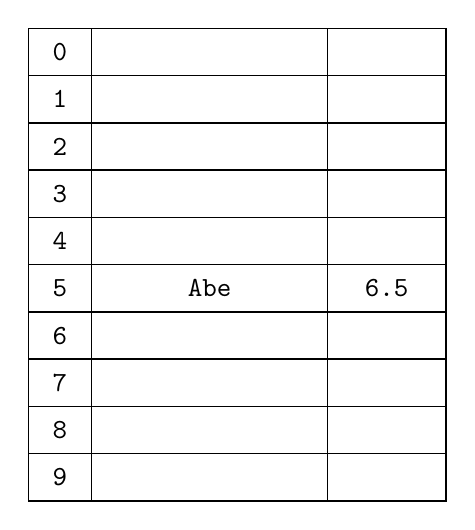
\begin{tikzpicture}

\draw (1.4, 0.7)
  node[draw, line width=0.02cm, , color=black,
       rounded corners=0cm, inner sep=0cm] {

\begin{minipage}[t][0.6cm]{0.8cm}
\mbox{}

\end{minipage}

};\draw (1.4, 0.7) node[color=black] {{\texttt{0}}};
\draw (3.3, 0.7)
  node[draw, line width=0.02cm, , color=black,
       rounded corners=0cm, inner sep=0cm] {

\begin{minipage}[t][0.6cm]{3.0cm}
\mbox{}

\end{minipage}

};\draw (3.3, 0.7) node[color=black] {{\texttt{}}};
\draw (5.55, 0.7)
  node[draw, line width=0.02cm, , color=black,
       rounded corners=0cm, inner sep=0cm] {

\begin{minipage}[t][0.6cm]{1.5cm}
\mbox{}

\end{minipage}

};\draw (5.55, 0.7) node[color=black] {{\texttt{}}};
\draw (1.4, 0.09999999999999987)
  node[draw, line width=0.02cm, , color=black,
       rounded corners=0cm, inner sep=0cm] {

\begin{minipage}[t][0.6cm]{0.8cm}
\mbox{}

\end{minipage}

};\draw (1.4, 0.09999999999999987) node[color=black] {{\texttt{1}}};
\draw (3.3, 0.09999999999999987)
  node[draw, line width=0.02cm, , color=black,
       rounded corners=0cm, inner sep=0cm] {

\begin{minipage}[t][0.6cm]{3.0cm}
\mbox{}

\end{minipage}

};\draw (3.3, 0.09999999999999987) node[color=black] {{\texttt{}}};
\draw (5.55, 0.09999999999999987)
  node[draw, line width=0.02cm, , color=black,
       rounded corners=0cm, inner sep=0cm] {

\begin{minipage}[t][0.6cm]{1.5cm}
\mbox{}

\end{minipage}

};\draw (5.55, 0.09999999999999987) node[color=black] {{\texttt{}}};
\draw (1.4, -0.5000000000000002)
  node[draw, line width=0.02cm, , color=black,
       rounded corners=0cm, inner sep=0cm] {

\begin{minipage}[t][0.6cm]{0.8cm}
\mbox{}

\end{minipage}

};\draw (1.4, -0.5000000000000002) node[color=black] {{\texttt{2}}};
\draw (3.3, -0.5000000000000002)
  node[draw, line width=0.02cm, , color=black,
       rounded corners=0cm, inner sep=0cm] {

\begin{minipage}[t][0.6cm]{3.0cm}
\mbox{}

\end{minipage}

};\draw (3.3, -0.5000000000000002) node[color=black] {{\texttt{}}};
\draw (5.55, -0.5000000000000002)
  node[draw, line width=0.02cm, , color=black,
       rounded corners=0cm, inner sep=0cm] {

\begin{minipage}[t][0.6cm]{1.5cm}
\mbox{}

\end{minipage}

};\draw (5.55, -0.5000000000000002) node[color=black] {{\texttt{}}};
\draw (1.4, -1.1000000000000003)
  node[draw, line width=0.02cm, , color=black,
       rounded corners=0cm, inner sep=0cm] {

\begin{minipage}[t][0.6cm]{0.8cm}
\mbox{}

\end{minipage}

};\draw (1.4, -1.1000000000000003) node[color=black] {{\texttt{3}}};
\draw (3.3, -1.1000000000000003)
  node[draw, line width=0.02cm, , color=black,
       rounded corners=0cm, inner sep=0cm] {

\begin{minipage}[t][0.6cm]{3.0cm}
\mbox{}

\end{minipage}

};\draw (3.3, -1.1000000000000003) node[color=black] {{\texttt{}}};
\draw (5.55, -1.1000000000000003)
  node[draw, line width=0.02cm, , color=black,
       rounded corners=0cm, inner sep=0cm] {

\begin{minipage}[t][0.6cm]{1.5cm}
\mbox{}

\end{minipage}

};\draw (5.55, -1.1000000000000003) node[color=black] {{\texttt{}}};
\draw (1.4, -1.7000000000000002)
  node[draw, line width=0.02cm, , color=black,
       rounded corners=0cm, inner sep=0cm] {

\begin{minipage}[t][0.6cm]{0.8cm}
\mbox{}

\end{minipage}

};\draw (1.4, -1.7000000000000002) node[color=black] {{\texttt{4}}};
\draw (3.3, -1.7000000000000002)
  node[draw, line width=0.02cm, , color=black,
       rounded corners=0cm, inner sep=0cm] {

\begin{minipage}[t][0.6cm]{3.0cm}
\mbox{}

\end{minipage}

};\draw (3.3, -1.7000000000000002) node[color=black] {{\texttt{}}};
\draw (5.55, -1.7000000000000002)
  node[draw, line width=0.02cm, , color=black,
       rounded corners=0cm, inner sep=0cm] {

\begin{minipage}[t][0.6cm]{1.5cm}
\mbox{}

\end{minipage}

};\draw (5.55, -1.7000000000000002) node[color=black] {{\texttt{}}};
\draw (1.4, -2.3000000000000003)
  node[draw, line width=0.02cm, , color=black,
       rounded corners=0cm, inner sep=0cm] {

\begin{minipage}[t][0.6cm]{0.8cm}
\mbox{}

\end{minipage}

};\draw (1.4, -2.3000000000000003) node[color=black] {{\texttt{5}}};
\draw (3.3, -2.3000000000000003)
  node[draw, line width=0.02cm, , color=black,
       rounded corners=0cm, inner sep=0cm] {

\begin{minipage}[t][0.6cm]{3.0cm}
\mbox{}

\end{minipage}

};\draw (3.3, -2.3000000000000003) node[color=black] {{\texttt{Abe}}};
\draw (5.55, -2.3000000000000003)
  node[draw, line width=0.02cm, , color=black,
       rounded corners=0cm, inner sep=0cm] {

\begin{minipage}[t][0.6cm]{1.5cm}
\mbox{}

\end{minipage}

};\draw (5.55, -2.3000000000000003) node[color=black] {{\texttt{6.5}}};
\draw (1.4, -2.9000000000000004)
  node[draw, line width=0.02cm, , color=black,
       rounded corners=0cm, inner sep=0cm] {

\begin{minipage}[t][0.6cm]{0.8cm}
\mbox{}

\end{minipage}

};\draw (1.4, -2.9000000000000004) node[color=black] {{\texttt{6}}};
\draw (3.3, -2.9000000000000004)
  node[draw, line width=0.02cm, , color=black,
       rounded corners=0cm, inner sep=0cm] {

\begin{minipage}[t][0.6cm]{3.0cm}
\mbox{}

\end{minipage}

};\draw (3.3, -2.9000000000000004) node[color=black] {{\texttt{}}};
\draw (5.55, -2.9000000000000004)
  node[draw, line width=0.02cm, , color=black,
       rounded corners=0cm, inner sep=0cm] {

\begin{minipage}[t][0.6cm]{1.5cm}
\mbox{}

\end{minipage}

};\draw (5.55, -2.9000000000000004) node[color=black] {{\texttt{}}};
\draw (1.4, -3.500000000000001)
  node[draw, line width=0.02cm, , color=black,
       rounded corners=0cm, inner sep=0cm] {

\begin{minipage}[t][0.6cm]{0.8cm}
\mbox{}

\end{minipage}

};\draw (1.4, -3.500000000000001) node[color=black] {{\texttt{7}}};
\draw (3.3, -3.500000000000001)
  node[draw, line width=0.02cm, , color=black,
       rounded corners=0cm, inner sep=0cm] {

\begin{minipage}[t][0.6cm]{3.0cm}
\mbox{}

\end{minipage}

};\draw (3.3, -3.500000000000001) node[color=black] {{\texttt{}}};
\draw (5.55, -3.500000000000001)
  node[draw, line width=0.02cm, , color=black,
       rounded corners=0cm, inner sep=0cm] {

\begin{minipage}[t][0.6cm]{1.5cm}
\mbox{}

\end{minipage}

};\draw (5.55, -3.500000000000001) node[color=black] {{\texttt{}}};
\draw (1.4, -4.1000000000000005)
  node[draw, line width=0.02cm, , color=black,
       rounded corners=0cm, inner sep=0cm] {

\begin{minipage}[t][0.6cm]{0.8cm}
\mbox{}

\end{minipage}

};\draw (1.4, -4.1000000000000005) node[color=black] {{\texttt{8}}};
\draw (3.3, -4.1000000000000005)
  node[draw, line width=0.02cm, , color=black,
       rounded corners=0cm, inner sep=0cm] {

\begin{minipage}[t][0.6cm]{3.0cm}
\mbox{}

\end{minipage}

};\draw (3.3, -4.1000000000000005) node[color=black] {{\texttt{}}};
\draw (5.55, -4.1000000000000005)
  node[draw, line width=0.02cm, , color=black,
       rounded corners=0cm, inner sep=0cm] {

\begin{minipage}[t][0.6cm]{1.5cm}
\mbox{}

\end{minipage}

};\draw (5.55, -4.1000000000000005) node[color=black] {{\texttt{}}};
\draw (1.4, -4.7)
  node[draw, line width=0.02cm, , color=black,
       rounded corners=0cm, inner sep=0cm] {

\begin{minipage}[t][0.6cm]{0.8cm}
\mbox{}

\end{minipage}

};\draw (1.4, -4.7) node[color=black] {{\texttt{9}}};
\draw (3.3, -4.7)
  node[draw, line width=0.02cm, , color=black,
       rounded corners=0cm, inner sep=0cm] {

\begin{minipage}[t][0.6cm]{3.0cm}
\mbox{}

\end{minipage}

};\draw (3.3, -4.7) node[color=black] {{\texttt{}}};
\draw (5.55, -4.7)
  node[draw, line width=0.02cm, , color=black,
       rounded corners=0cm, inner sep=0cm] {

\begin{minipage}[t][0.6cm]{1.5cm}
\mbox{}

\end{minipage}

};\draw (5.55, -4.7) node[color=black] {{\texttt{}}};
\end{tikzpicture}

\end{center}



%-*-latex-*-

\begin{ex} 
  \label{ex:prob-00}
  \tinysidebar{\debug{exercises/{disc-prob-28/question.tex}}}

  \solutionlink{sol:prob-00}
  \qed
\end{ex} 
\begin{python0}
from solutions import *
add(label="ex:prob-00",
    srcfilename='exercises/discrete-probability/prob-00/answer.tex') 
\end{python0}


Of course if your \verb!N! is really, really, really huge,
you will find that the probability of getting a head is 0.5 and 
the probability of getting a tail is 0.5.

Here's a function (derived by simulation) 
that gives us the probability for each possible outcome
of our experiment:
\includesourcenonumbers{tossfaircoin3.py}
I've increase \verb!n! to 1000 and 
also commented out the printing of each experiment.
Here's my output when I run the program:
\begin{center}
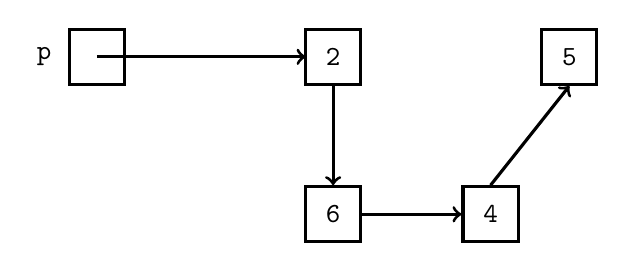
\begin{tikzpicture}

\draw (0.35, 0.35)
  node[draw, line width=0.04cm, , color=black,
       rounded corners=0cm, inner sep=0cm] {

\begin{minipage}[t][0.7cm]{0.7cm}
\mbox{}

\end{minipage}

};\draw (0.35, 0.35) node[color=black] {{\texttt{2}}};
\draw (0.35, -1.65)
  node[draw, line width=0.04cm, , color=black,
       rounded corners=0cm, inner sep=0cm] {

\begin{minipage}[t][0.7cm]{0.7cm}
\mbox{}

\end{minipage}

};\draw (0.35, -1.65) node[color=black] {{\texttt{6}}};
\draw (2.35, -1.65)
  node[draw, line width=0.04cm, , color=black,
       rounded corners=0cm, inner sep=0cm] {

\begin{minipage}[t][0.7cm]{0.7cm}
\mbox{}

\end{minipage}

};\draw (2.35, -1.65) node[color=black] {{\texttt{4}}};
\draw (3.35, 0.35)
  node[draw, line width=0.04cm, , color=black,
       rounded corners=0cm, inner sep=0cm] {

\begin{minipage}[t][0.7cm]{0.7cm}
\mbox{}

\end{minipage}

};\draw (3.35, 0.35) node[color=black] {{\texttt{5}}};\draw[line width=0.04cm,black,->] (0.35,-0.02) to  (0.35,-1.28);
\draw[line width=0.04cm,black,->] (0.72,-1.65) to  (1.98,-1.65);
\draw[line width=0.04cm,black,->] (2.35,-1.28) to  (3.35,-0.02);

\draw (-2.65, 0.35)
  node[draw, line width=0.04cm, , color=black,
       rounded corners=0cm, inner sep=0cm] {

\begin{minipage}[t][0.7cm]{0.7cm}
\mbox{}

\end{minipage}

};\draw (-2.65, 0.35) node[color=black] {{\texttt{}}};\draw[line width=0.04cm,black,->] (-2.65,0.35) to  (0,0.35);

\draw (-3.32, 0.35)
  node[draw, line width=0.04cm, , color=white,
       rounded corners=0cm, inner sep=0cm] {

\begin{minipage}[t][0.1cm]{0.1cm}
\mbox{}

\end{minipage}

};\draw (-3.32, 0.35) node[color=black] {{\texttt{p}}};
\end{tikzpicture}

\end{center}



Of course if we assume from the beginning that our coin is fair we can 
save the trouble of the computation:
\includesourcenonumbers{tossfaircoin4.py}
Here's my output when I run the program:
\begin{center}
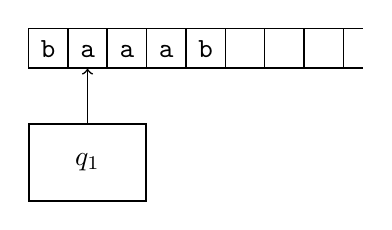
\begin{tikzpicture}

\draw (0.25, 0.25)
  node[draw, line width=0.02cm, , color=black,
       rounded corners=0cm, inner sep=0cm] {

\begin{minipage}[t][0.5cm]{0.5cm}
\mbox{}

\end{minipage}

};\draw (0.25, 0.25) node[color=black] {{\vphantom{baaab\SPACE\SPACE\SPACE}\texttt{b}}};
\draw (0.75, 0.25)
  node[draw, line width=0.02cm, , color=black,
       rounded corners=0cm, inner sep=0cm] {

\begin{minipage}[t][0.5cm]{0.5cm}
\mbox{}

\end{minipage}

};\draw (0.75, 0.25) node[color=black] {{\vphantom{baaab\SPACE\SPACE\SPACE}\texttt{a}}};
\draw (1.25, 0.25)
  node[draw, line width=0.02cm, , color=black,
       rounded corners=0cm, inner sep=0cm] {

\begin{minipage}[t][0.5cm]{0.5cm}
\mbox{}

\end{minipage}

};\draw (1.25, 0.25) node[color=black] {{\vphantom{baaab\SPACE\SPACE\SPACE}\texttt{a}}};
\draw (1.75, 0.25)
  node[draw, line width=0.02cm, , color=black,
       rounded corners=0cm, inner sep=0cm] {

\begin{minipage}[t][0.5cm]{0.5cm}
\mbox{}

\end{minipage}

};\draw (1.75, 0.25) node[color=black] {{\vphantom{baaab\SPACE\SPACE\SPACE}\texttt{a}}};
\draw (2.25, 0.25)
  node[draw, line width=0.02cm, , color=black,
       rounded corners=0cm, inner sep=0cm] {

\begin{minipage}[t][0.5cm]{0.5cm}
\mbox{}

\end{minipage}

};\draw (2.25, 0.25) node[color=black] {{\vphantom{baaab\SPACE\SPACE\SPACE}\texttt{b}}};
\draw (2.75, 0.25)
  node[draw, line width=0.02cm, , color=black,
       rounded corners=0cm, inner sep=0cm] {

\begin{minipage}[t][0.5cm]{0.5cm}
\mbox{}

\end{minipage}

};\draw (2.75, 0.25) node[color=black] {{\vphantom{baaab\SPACE\SPACE\SPACE}\texttt{\SPACE}}};
\draw (3.25, 0.25)
  node[draw, line width=0.02cm, , color=black,
       rounded corners=0cm, inner sep=0cm] {

\begin{minipage}[t][0.5cm]{0.5cm}
\mbox{}

\end{minipage}

};\draw (3.25, 0.25) node[color=black] {{\vphantom{baaab\SPACE\SPACE\SPACE}\texttt{\SPACE}}};
\draw (3.75, 0.25)
  node[draw, line width=0.02cm, , color=black,
       rounded corners=0cm, inner sep=0cm] {

\begin{minipage}[t][0.5cm]{0.5cm}
\mbox{}

\end{minipage}

};\draw (3.75, 0.25) node[color=black] {{\vphantom{baaab\SPACE\SPACE\SPACE}\texttt{\SPACE}}};\draw[line width=0.02cm,black] (4.0,0.5) to  (4.25,0.5);
\draw[line width=0.02cm,black] (4.0,0.0) to  (4.25,0.0);

\draw (0.75, -1.2)
  node[draw, line width=0.02cm, , color=black,
       rounded corners=0cm, inner sep=0cm] {

\begin{minipage}[t][0.98cm]{1.48cm}
\mbox{}

\end{minipage}

};\draw (0.75, -1.2) node[color=black] {$q_1$};\draw[line width=0.02cm,black,->] (0.75,-0.7) to  (0.75,-0.47) to  (0.75,-0.47) to  (0.75,-0.01);
\end{tikzpicture}

\end{center}



Of course when \verb!n! gets larger and larger, the probability function
derived using simulations will match this new \lq\lq theoretically'' derived
function.

%-*-latex-*-

\begin{ex} 
  \label{ex:prob-00}
  \tinysidebar{\debug{exercises/{disc-prob-28/question.tex}}}

  \solutionlink{sol:prob-00}
  \qed
\end{ex} 
\begin{python0}
from solutions import *
add(label="ex:prob-00",
    srcfilename='exercises/discrete-probability/prob-00/answer.tex') 
\end{python0}

%-*-latex-*-

\begin{ex} 
  \label{ex:prob-00}
  \tinysidebar{\debug{exercises/{disc-prob-28/question.tex}}}

  \solutionlink{sol:prob-00}
  \qed
\end{ex} 
\begin{python0}
from solutions import *
add(label="ex:prob-00",
    srcfilename='exercises/discrete-probability/prob-00/answer.tex') 
\end{python0}

%-*-latex-*-

\begin{ex} 
  \label{ex:prob-00}
  \tinysidebar{\debug{exercises/{disc-prob-28/question.tex}}}

  \solutionlink{sol:prob-00}
  \qed
\end{ex} 
\begin{python0}
from solutions import *
add(label="ex:prob-00",
    srcfilename='exercises/discrete-probability/prob-00/answer.tex') 
\end{python0}


I abstract the coin toss experiment as follows:
Let $S = \{\HEAD, \TAIL\}$ represent all possible outcomes of
my coin toss experiment.
$S$ is the called the \defone{sample space} of my random experiment.
$\HEAD$ and $\TAIL$ are called
the \defone{outcomes} of my experiment.
I define a function
\[
  p : S \rightarrow \R 
\]
such that $p(\HEAD)$ gives us the chance that
a coin toss will give us a head and
$p(\TAIL)$ gives us the chance of getting a tail.
So if the coin is fair, I would have
\[
  p(\HEAD) = 1/2 = p(\TAIL)
\]
$p$ is called a
\defterm{probability distribution function}\index{probability distribution function}\tinysidebar{probability distribution function \\ pdf}
(\defterm{pdf}\index{pdf}):
it distributes $1$ to all outcomes:
\[
1 = p(\HEAD) + p(\TAIL) = \sum_{x \in S} p(x)
\]
$p$ is also called a
\defterm{probability function}\index{probability function}\tinysidebar{probability function \\ probability mass function}
or a 
\defterm{probability mass function}\index{probability mass function}.




\newpage
\subsection{Die rolls}

When you roll a die, you get the face value of the roll, i.e.,
the number of dots on the top surface of the die, you
get one of the following:
\[
\text{
\texttt{ONE},
\texttt{TWO},
\texttt{THREE},
\texttt{FOUR},
\texttt{FIVE},
\texttt{SIX},
}
\]
Assuming that the die is fair and you roll the die a huge
number of times, you will see that approximately 1/6 of the 
rolls will give you a \texttt{ONE}
(and likewise for the other cases.)

I can assign 1/6 to \texttt{ONE} to indicate that the 
proportion of rolls that gives me \texttt{ONE}.
Likewise for the other cases.
This is basically a function
\[
p : \{\texttt{ONE},
\texttt{TWO},
\texttt{THREE},
\texttt{FOUR},
\texttt{FIVE},
\texttt{SIX}
\}
\rightarrow [0,1]
\]
such that 
\begin{align*}
p(\texttt{ONE}) &= 1/6 \\
p(\texttt{TWO}) &= 1/6 \\
p(\texttt{THREE}) &= 1/6 \\
p(\texttt{FOUR}) &= 1/6 \\
p(\texttt{FIVE}) &= 1/6 \\
p(\texttt{SIX}) &= 1/6
\end{align*}
As in the previous subsection, the set 
$S = \{
\texttt{ONE},
\texttt{TWO},
\texttt{THREE},
\texttt{FOUR},
\texttt{FIVE},
\texttt{SIX}
\}$ 
is called the set of outcomes or the sample space
of my experiment of rolling a die.
Note that
\[
\sum_{x \in S} p(x) = 1
\]

For us, our sample space is a finite set (you can also 
talk about probability theory for non-finite sets.) 


%-*-latex-*-

\begin{ex} 
  \label{ex:prob-00}
  \tinysidebar{\debug{exercises/{disc-prob-28/question.tex}}}

  \solutionlink{sol:prob-00}
  \qed
\end{ex} 
\begin{python0}
from solutions import *
add(label="ex:prob-00",
    srcfilename='exercises/discrete-probability/prob-00/answer.tex') 
\end{python0}

%-*-latex-*-

\begin{ex} 
  \label{ex:prob-00}
  \tinysidebar{\debug{exercises/{disc-prob-28/question.tex}}}

  \solutionlink{sol:prob-00}
  \qed
\end{ex} 
\begin{python0}
from solutions import *
add(label="ex:prob-00",
    srcfilename='exercises/discrete-probability/prob-00/answer.tex') 
\end{python0}


A probability distribution function is \defone{uniform}
if $p(x)$ is the same for all $x$ in the sample space of the function.
When I say that I'm rolling a \defone{fair} die, I mean that the probability
function for the experiment (of rolling the die) is uniform.

%-*-latex-*-

\begin{ex} 
  \label{ex:prob-00}
  \tinysidebar{\debug{exercises/{disc-prob-28/question.tex}}}

  \solutionlink{sol:prob-00}
  \qed
\end{ex} 
\begin{python0}
from solutions import *
add(label="ex:prob-00",
    srcfilename='exercises/discrete-probability/prob-00/answer.tex') 
\end{python0}


Instead of asking the probability of getting a \texttt{SIX} when
I roll a die, I might be interested in getting \texttt{ONE} or \texttt{SIX}.
In general, a subset $A$ of the set of all outcomes is called an 
\defone{event}.
In that case, I will write $p(A)$ or $p[A]$ for
\[
p(A) = \sum_{x \in A} p(x)
\]
So for instance in the case of our die,
\[
p[\{\texttt{ONE}, \texttt{SIX}\}]
= p(\texttt{ONE}) + p(\texttt{SIX})
= 1/6 + 1/6 = 1/3
\]

Let $A$ and $B$ be events of an experiment with sample space $S$
and probability distribution function $p$.
Then
\[
p[A \cup B] \leq p[A] + p[B]
\]
This means that if we know a lot about the probability of $A$ and 
probability of $B$, but we're not very sure about the common
events of $A$ and $B$, we can still bound the probability of $A \cup B$.
If we do know something about the probability of $A \cap B$, then we have
\[
p[A \cup B] = p[A] + p[B] - p[A \cap B]
\]

If $A \cap B = \emptyset$, we get
\[
p[A \cup B] = p[A] + p[B]
\]
Clearly we also have
\[
p[\emptyset] = 0
\]
and
\[
p[S] = 1
\]

Clearly
\[
p[\overline{A}] = 1 - p[A]
\]
where $\overline{A} = S - A$ is the complement of $A$ (with respect to $S$).

\newpage%-*-latex-*-
\sectionthree{Experimental (or Empirical) Approach}
\begin{python0}
from solutions import *; clear()
\end{python0}

Here's how to think of probability intuitively:
You can of course think of probability as some kind of averaging.
In the case of tossing a particular coin, if you say
\[
p(\HEAD) = \frac{1}{3}
\]
what you meant is that if you toss the coin 3 times, then
it's likely that 
approximately 1 out of the 3 is a head;
if you toss the coin 300 times, then it's very likely that
approximately 100 of the 300 are heads;
if you toss the coin 3000 times, then it's very very likely that
approximately 1000 of the 3000 are heads; etc.
The more tosses you make, the closer you get to \lq\lq one third of the
tosses comes out head''.

In the above coin toss experiment, I have two possible outcomes:
either I get a head or I get a tail.
I create two symbols to represent these two possible outcomes:
$\HEAD$ and $\TAIL$.
The names is arbitrary and it's entirely up to you to come up with
symbols for all the possible outcomes.
For instance you can name the outcomes H and T instead of
$\HEAD$ and $\TAIL$.

How let's formalize the notation for studying probability theory ...


\newpage%-*-latex-*-
\section{Probability distribution function}

A (finite) discrete 
\defone{probability distribution function} is
a 
real-valued function on a finite set $S$ 
\[
p : S \rightarrow \R
\]
such that 
\begin{axioms}
\item[{[DP-1]}] $0 \leq p(x) \leq 1$ for all $x \in S$
\item[{[DP-2]}] $\sum_{x \in S} p(x) = 1$
\end{axioms}
$S$ is a
\defterm{sample space}\index{sample space}\tinysidebar{sample space \\ outcomes}.
The elements of $S$ are called
\defterm{outcomes}\index{outcomes},
Because of [DP-1], I can change the codmain of $p$:
\[
p : S \rightarrow [0,1]
\]
A subset of $S$ is called an \defone{event}.
If $A$ is a subset of $S$, I'll write
\[
p(A) = \sum_{x \in A} p(x)
\]
[DP-2] is the same as saying
\[
p(S) = 1
\]

Here are some basic facts about pdfs.


%-*-latex-*-

\begin{ex} 
  \label{ex:prob-00}
  \tinysidebar{\debug{exercises/{disc-prob-28/question.tex}}}

  \solutionlink{sol:prob-00}
  \qed
\end{ex} 
\begin{python0}
from solutions import *
add(label="ex:prob-00",
    srcfilename='exercises/discrete-probability/prob-00/answer.tex') 
\end{python0}



\begin{defn}
A probability distribution function $p : S \rightarrow [0,1]$ 
is said to be \defone{uniform} if
\[
p(x) = \frac{1}{|S|}
\]
for each $x \in S$.
$|S|$, the size of $S$, denotes the numbers of distinct elements in $S$.
\end{defn}

\begin{eg}
Suppose that I've rigged my coin so that the chance of getting
a head is twice of getting the tail.
This means that the probability function
\[
p : S \rightarrow [0,1]
\]
is
\[
p(\HEAD) = \frac{2}{3}, \,\,\,\,\,
p(\TAIL) = \frac{1}{3} \,\,\,\,\,
\]
Of course if the coin is a fair coin I would have
\[
p(\HEAD) = \frac{1}{2} = p(\TAIL)
\]
\qed
\end{eg}


%-*-latex-*-

\begin{ex} 
  \label{ex:prob-00}
  \tinysidebar{\debug{exercises/{disc-prob-28/question.tex}}}

  \solutionlink{sol:prob-00}
  \qed
\end{ex} 
\begin{python0}
from solutions import *
add(label="ex:prob-00",
    srcfilename='exercises/discrete-probability/prob-00/answer.tex') 
\end{python0}



\begin{eg}
Suppose I have a loaded die such that getting a \lq\lq 1'' 
is 10 times more likely 
than the others and the others are equally likely.
Let $p$ be the probability function of rolling this die.
Then
\begin{align*}
1 
&= p(\ONE) + p(\TWO) + \cdots + p(\SIX) \\
&= p(\ONE) + 5 \cdot p(\TWO) \\
&= p(\ONE) + 5 \cdot \frac{1}{10} p(\ONE) \\
&= \frac{3}{2} \cdot p(\ONE) 
\end{align*}
So 
\[
p(\ONE) = \frac{2}{3}
\]
and 
\[
p(\TWO) = p(\THREE) = ... = p(\SIX) = \frac{2}{30}
\]
And of course
\[
S = \{\ONE, \TWO, \THREE, \FOUR, \FIVE, \SIX\}
\]

Go ahead and write a program to simulate tossing my loaded die.
Run it for a large number of experiments and check that you get the
expected results. 
\begin{Verbatim}[fontsize=\small, frame=single]
import random; random.seed()

ONE = "ONE"
TWO = "TWO"
THREE = "THREE"
FOUR = "FOUR"
FIVE = "FIVE"
SIX = "SIX"

# write a probability function for this experiment

def roll_die():
    r = random.randrange(30)
    if r < 20: return ONE
    elif r < 22: return TWO
    elif r < 24: return THREE
    elif r < 26: return FOUR
    elif r < 28: return FIVE
    else: return SIX

NUM_EXPERIMENTS = 20
for i in range(NUM_EXPERIMENTS):
    print("experiment", i, "... outcome:", roll_die())
\end{Verbatim}
\end{eg}


The following function can be used to produce the different
experiment functions (you should type it up and run it ... if you're
too lazy to do that you can also grab the code from
our class web site ... look for \lq\lq probability library"):
\begin{Verbatim}[frame=single, fontsize=\small]
def build_experiment(xs):
    total = sum([b for (a,b) in xs])
    accumulate = xs[0]
    for (a,b) in xs[1:]:
        accumulate.append((a, accumulate[-1][1] + b)
    def experiment():
        r = random.randrange(total)
        for (a,b) in accumulate:
            if r < b: return a
        raise ValueError("r:%s greater than total:%s" %\
                         (r, total))
    return experiment

HEAD = "HEAD"
TAIL = "TAIL"
toss_coin = build_experiment([(HEAD, 2),
                              (TAIL, 1),
                             ])
ONE = "ONE"
TWO = "TWO"
THREE = "THREE"
FOUR = "FOUR"
FIVE = "FIVE"
SIX = "SIX"
roll_die = build_experiment([(ONE, 20),
                             (TWO, 2),
                             (THREE, 2),
                             (FOUR, 2),
                             (FIVE, 2),
                             (SIX, 2),
                            ])
\end{Verbatim}

%-*-latex-*-

\begin{ex} 
  \label{ex:prob-00}
  \tinysidebar{\debug{exercises/{disc-prob-28/question.tex}}}

  \solutionlink{sol:prob-00}
  \qed
\end{ex} 
\begin{python0}
from solutions import *
add(label="ex:prob-00",
    srcfilename='exercises/discrete-probability/prob-00/answer.tex') 
\end{python0}

%-*-latex-*-

\begin{ex} 
  \label{ex:prob-00}
  \tinysidebar{\debug{exercises/{disc-prob-28/question.tex}}}

  \solutionlink{sol:prob-00}
  \qed
\end{ex} 
\begin{python0}
from solutions import *
add(label="ex:prob-00",
    srcfilename='exercises/discrete-probability/prob-00/answer.tex') 
\end{python0}


Now what is asked is actually related to another
experiment: 
\lq\lq Attend 3 classes in a row''.
(Later you'll see how to view this as a \lq\lq product of
experiments''.)
There are two ways to compute an approximation of the desired
probability.

FIRST METHOD:
You should use the first experiment to generate a sequence of
$\mathsc{Q}$'s and
$\mathsc{N}$'s:
\[
\mathsc{Q},
\mathsc{Q},
\mathsc{N},
\mathsc{Q},
\mathsc{Q},
\mathsc{Q},
\mathsc{Q},
\mathsc{Q},
\mathsc{Q},
\mathsc{N},
\mathsc{Q},
\mathsc{Q},
...
\]
satisfying the given probability that
$p(\mathsc{Q}) = 0.8$ and
$p(\mathsc{N}) = 0.2$.
Next you look at all the consecutive triples.
For instance the above gives
\[
\mathsc{QQN},
\mathsc{QNQ},
\mathsc{NQQ},
\mathsc{QQQ},
\mathsc{QQQ},
\mathsc{QQQ},
\mathsc{QQQ},
\mathsc{QQQ},
\mathsc{QQN},
\mathsc{QNQ},
\mathsc{NQQ}, ...
\]
and then compute the approximate probability of seeing
$\mathsc{QQQ}$ in 
this sampling.
Of course you need to have a reasonbly huge sample.
You can either do this by hand or write a program to simulate the
experiment.

SECOND METHOD:
If you have a function for the first experiment, say
\verb!attend_class! which gives you $\mathsc{Q}$ or
$\mathsc{N}$, then you should have a
function say \verb!attend_3_classes! that uses \verb!attend_class!:
\begin{Verbatim}[frame=single]
Q = 'Q'
N = 'N'

def attend_3_classes():
    return [attend_class(), 
            attend_class(), 
            attend_class(),
           ]
\end{Verbatim}
Of course you can now generate samples and count:
\begin{Verbatim}[frame=single]
MAX = 100000
count = 0
for i in range(MAX):
    if attend_3_classes() == [Q, Q, Q]: 
        count += 1
print(float(count) / MAX)
\end{Verbatim}

%-*-latex-*-

\begin{ex} 
  \label{ex:prob-00}
  \tinysidebar{\debug{exercises/{disc-prob-28/question.tex}}}

  \solutionlink{sol:prob-00}
  \qed
\end{ex} 
\begin{python0}
from solutions import *
add(label="ex:prob-00",
    srcfilename='exercises/discrete-probability/prob-00/answer.tex') 
\end{python0}


\newpage%-*-latex-*-
\sectionthree{Random variable}
\begin{python0}
from solutions import *; clear()
\end{python0}

Now for the definition of a very confusing term: random variable.
A \defone{random variable} $X$ of $S$ (a sample space) is just a function
from $S$ to some set, say $V$.
\[
  X : S \rightarrow V
\]
Usually $V$ is the set of real numbers:
\[
  X : S \rightarrow \R
\]
It's really important to remember that a random variable
is not random and is not a variable!!!
It's just a function from a sample space to a set.
This is an example of a badly chosen name for this idea.

There are two main reasons why we need the concept of random variables.
Pay attention to the following.



\newpage
\subsection{Random variable as labels}

The first reason for having random variables is
that we want to create some 
labels for the values in a sample space.
The labels will then create subsets of the sample space, i.e.,
random variables helps create meaningful events.

As an example, I'm going back to the die roll experiment.
The sample space is
\[
S = \{\ONE, \TWO, \THREE, \FOUR, \FIVE, \SIX \}
\]
Suppose I'm playing a game with a die and I win
if the roll gives me either $\ONE$ or $\SIX$;
otherwise I lose.
I can then define the following
random variables:
\[
  X : \{ \ONE, ..., \SIX \} \rightarrow \{ \GOOD, \BAD \}
\]
where
\begin{align*}
  X(\ONE) &= X(\SIX) = \textsc{Good} \\
  X(\TWO) &= X(\THREE) = X(\FOUR) = X(\FIVE) = \BAD 
\end{align*}
We have create two subsets
\begin{align*}
  A &= \{ s \in S \mid X(s) = \GOOD \} \\
  B &= \{ s \in S \mid X(s) = \BAD \}
\end{align*}
of $S$.
In other words, random variables create events for each
value in the range of the random variables.
In fact the subsets created are disjoint
and the union of all these subsets for the original
sample space.
In other words, $X$ creates a partition of the sample space,
i.e., $A$ and $B$ are disjoint and $A \cup B$ is $X$.

As a consequence, my random variable $X$ also defines a new
probability distribution function
\[
  p_X : \{ \GOOD, \BAD \} \rightarrow [0,1]
\]
where
\begin{align*}
  p_X(\GOOD) &= p(\{ s \in S \mid X(s) = \GOOD \}) = 1/3 \\
  p_X(\BAD) &= p(\{ s \in S \mid X(s) = \BAD \}) = 2/3
\end{align*}
This function is very frequently written like this:
\begin{align*}
  \Pr[X = \GOOD] &= 1/3 \\
  \Pr[X = \BAD] &= 2/3
\end{align*}
or sometimes
$\operatorname{P}[X=\GOOD]$
or
$\operatorname{P}(X=\GOOD)$.
This $\Pr$ is a bad notation because this function
actually depends on $p$ and $X$.
But nobody write $\Pr_p[X = \GOOD]$.
Part of the reason is because a random variable $X$
is usually tied to a probability distribution function.
Which is not exactly true since $X$ is a function of
the sample space and is therefore tied to the sample space
and not the probability function itself.
But this is the practice and you have to remember what I said
above in order not to be confused.

It's important to note that $p_X$ and $\Pr[X= \bullet]$ are pdfs,
but they are \textit{not} pdf on $S$: they are pdfs on
$\{ \GOOD, \BAD \}$.

Here's a picture to keep in mind:
%-*-latex-*-
\begin{center}
\begin{tikzpicture}

\draw (0.625, 0.25)
  node[draw=none, line width=0cm, , color=black,
       rounded corners=0cm, inner sep=0cm,
       name=1] {

\begin{minipage}[t][0.5cm]{1.25cm}
\mbox{}

\end{minipage}

};\draw (0.625, 0.25) node[color=black] {$\ONE$};
\draw (0.625, -0.25)
  node[draw=none, line width=0cm, , color=black,
       rounded corners=0cm, inner sep=0cm,
       name=2] {

\begin{minipage}[t][0.5cm]{1.25cm}
\mbox{}

\end{minipage}

};\draw (0.625, -0.25) node[color=black] {$\TWO$};
\draw (0.625, -0.75)
  node[draw=none, line width=0cm, , color=black,
       rounded corners=0cm, inner sep=0cm,
       name=3] {

\begin{minipage}[t][0.5cm]{1.25cm}
\mbox{}

\end{minipage}

};\draw (0.625, -0.75) node[color=black] {$\THREE$};
\draw (0.625, -1.25)
  node[draw=none, line width=0cm, , color=black,
       rounded corners=0cm, inner sep=0cm,
       name=4] {

\begin{minipage}[t][0.5cm]{1.25cm}
\mbox{}

\end{minipage}

};\draw (0.625, -1.25) node[color=black] {$\FOUR$};
\draw (0.625, -1.75)
  node[draw=none, line width=0cm, , color=black,
       rounded corners=0cm, inner sep=0cm,
       name=5] {

\begin{minipage}[t][0.5cm]{1.25cm}
\mbox{}

\end{minipage}

};\draw (0.625, -1.75) node[color=black] {$\FIVE$};
\draw (0.625, -2.25)
  node[draw=none, line width=0cm, , color=black,
       rounded corners=0cm, inner sep=0cm,
       name=6] {

\begin{minipage}[t][0.5cm]{1.25cm}
\mbox{}

\end{minipage}

};\draw (0.625, -2.25) node[color=black] {$\SIX$};
\draw (4.5, -1.0)
  node[draw=none, line width=0cm, , color=black,
       rounded corners=0cm, inner sep=0cm,
       name=p] {

\begin{minipage}[t][0.5cm]{1cm}
\mbox{}

\end{minipage}

};\draw (4.5, -1.0) node[color=black] {$1/6$};\node [ellipse, draw=black, fit=(1) (2) (3) (4) (5) (6), line width=0.05cm, inner sep=0.0cm] {};\node [ellipse, draw=black, fit=(p), line width=0.05cm, inner sep=0.5cm] {};\draw[line width=0.04cm,black,->] (1) to  (p);
\draw[line width=0.04cm,black,->] (2) to  (p);
\draw[line width=0.04cm,black,->] (3) to  (p);
\draw[line width=0.04cm,black,->] (4) to  (p);
\draw[line width=0.04cm,black,->] (5) to  (p);
\draw[line width=0.04cm,black,->] (6) to  (p);

\draw (0.625, -3.75)
  node[draw=none, line width=0cm, , color=black,
       rounded corners=0cm, inner sep=0cm,
       name=g] {

\begin{minipage}[t][0.5cm]{1.25cm}
\mbox{}

\end{minipage}

};\draw (0.625, -3.75) node[color=black] {\textsc{\textblue{Good}}};
\draw (0.625, -4.25)
  node[draw=none, line width=0cm, , color=black,
       rounded corners=0cm, inner sep=0cm,
       name=b] {

\begin{minipage}[t][0.5cm]{1.25cm}
\mbox{}

\end{minipage}

};\draw (0.625, -4.25) node[color=black] {\textsc{\textred{Bad}}};\node [ellipse, draw=black, fit=(g) (b), line width=0.05cm, inner sep=0.0cm] {};
\draw (4.5, -3.75)
  node[draw=none, line width=0cm, , color=black,
       rounded corners=0cm, inner sep=0cm,
       name=13] {

\begin{minipage}[t][0.5cm]{1cm}
\mbox{}

\end{minipage}

};\draw (4.5, -3.75) node[color=black] {\textblue{$1/3$}};
\draw (4.5, -4.25)
  node[draw=none, line width=0cm, , color=black,
       rounded corners=0cm, inner sep=0cm,
       name=23] {

\begin{minipage}[t][0.5cm]{1cm}
\mbox{}

\end{minipage}

};\draw (4.5, -4.25) node[color=black] {\textred{$2/3$}};\node [ellipse, draw=black, fit=(13) (23), line width=0.05cm, inner sep=0.4cm] {};\draw[line width=0.04cm,blue,->] (g) to  (13);
\draw[line width=0.04cm,red,->] (b) to  (23);
\draw[line width=0.04cm,blue,->] (1) to [bend right=90]  (g);
\draw[line width=0.04cm,red,->] (2) to [bend right=90]  (b);
\draw[line width=0.04cm,red,->] (3) to [bend right=90]  (b);
\draw[line width=0.04cm,red,->] (4) to [bend right=90]  (b);
\draw[line width=0.04cm,red,->] (5) to [bend right=90]  (b);
\draw[line width=0.04cm,blue,->] (6) to [bend right=90]  (g);
\end{tikzpicture}

\end{center}



The function at the top is $p$ and the function
at the bottom is $\Pr[X = \bullet]$.
You can (and should) think of a random variable as
collecting probabilities given by $p$ into buckets.
You can think of it this way:

\begin{center}
\begin{tikzpicture}

\draw (0.625, 0.5)
  node[draw=none, line width=0cm, , color=black,
       rounded corners=0cm, inner sep=0cm,
       name=1] {

\begin{minipage}[t][1.0cm]{1.25cm}
\mbox{}

\end{minipage}

};\draw (0.625, 0.5) node[color=black] {$\ONE$};
\draw (0.625, 0.0)
  node[draw=none, line width=0cm, , color=black,
       rounded corners=0cm, inner sep=0cm,
       name=6] {

\begin{minipage}[t][1.0cm]{1.25cm}
\mbox{}

\end{minipage}

};\draw (0.625, 0.0) node[color=black] {$\SIX$};
\draw (0.625, -2.2)
  node[draw=none, line width=0cm, , color=black,
       rounded corners=0cm, inner sep=0cm,
       name=2] {

\begin{minipage}[t][1.0cm]{1.25cm}
\mbox{}

\end{minipage}

};\draw (0.625, -2.2) node[color=black] {$\TWO$};
\draw (0.625, -2.7)
  node[draw=none, line width=0cm, , color=black,
       rounded corners=0cm, inner sep=0cm,
       name=3] {

\begin{minipage}[t][1.0cm]{1.25cm}
\mbox{}

\end{minipage}

};\draw (0.625, -2.7) node[color=black] {$\THREE$};
\draw (0.625, -3.2)
  node[draw=none, line width=0cm, , color=black,
       rounded corners=0cm, inner sep=0cm,
       name=4] {

\begin{minipage}[t][1.0cm]{1.25cm}
\mbox{}

\end{minipage}

};\draw (0.625, -3.2) node[color=black] {$\FOUR$};
\draw (0.625, -3.7)
  node[draw=none, line width=0cm, , color=black,
       rounded corners=0cm, inner sep=0cm,
       name=5] {

\begin{minipage}[t][1.0cm]{1.25cm}
\mbox{}

\end{minipage}

};\draw (0.625, -3.7) node[color=black] {$\FIVE$};
\draw (4.5, 0.0)
  node[draw=none, line width=0cm, , color=black,
       rounded corners=0cm, inner sep=0cm,
       name=p] {

\begin{minipage}[t][0.5cm]{1cm}
\mbox{}

\end{minipage}

};\draw (4.5, 0.0) node[color=black] {$1/6$};\node [ellipse, draw=blue, fit=(1) (6), line width=0.05cm, inner sep=0.1cm] (good) {};\node [ellipse, draw=red, fit=(2) (3) (4) (5), line width=0.05cm, inner sep=0.1cm] (bad) {};\node [ellipse, draw=black, fit=(good) (bad), line width=0.05cm, inner sep=0.1cm] {};\node [ellipse, draw=black, fit=(p), line width=0.05cm, inner sep=0.5cm] {};\draw[line width=0.04cm,black,->] (1) to  (p);
\draw[line width=0.04cm,black,->] (2) to  (p);
\draw[line width=0.04cm,black,->] (3) to  (p);
\draw[line width=0.04cm,black,->] (4) to  (p);
\draw[line width=0.04cm,black,->] (5) to  (p);
\draw[line width=0.04cm,black,->] (6) to  (p);

\draw (4.5, -2.75)
  node[draw=none, line width=0cm, , color=black,
       rounded corners=0cm, inner sep=0cm,
       name=13] {

\begin{minipage}[t][0.5cm]{1cm}
\mbox{}

\end{minipage}

};\draw (4.5, -2.75) node[color=black] {\textblue{$1/3$}};
\draw (4.5, -3.25)
  node[draw=none, line width=0cm, , color=black,
       rounded corners=0cm, inner sep=0cm,
       name=23] {

\begin{minipage}[t][0.5cm]{1cm}
\mbox{}

\end{minipage}

};\draw (4.5, -3.25) node[color=black] {\textred{$2/3$}};\node [ellipse, draw=black, fit=(13) (23), line width=0.05cm, inner sep=0.4cm] {};\draw[line width=0.04cm,blue,->] (good) to  (13);
\draw[line width=0.04cm,red,->] (bad) to  (23);
\end{tikzpicture}

\end{center}



The random variable $X$ basically collects up probabilities:
$\ONE$ and $\SIX$ are collected up into \GOOD\
and the rest are collected up into \BAD.

It's possible, in fact it's common, to have multiple
random variables on the same sample space.

Here's another random variable:
\[
Y : S \rightarrow \{ \EVEN, \ODD \}
\]
where
\begin{align*}
Y(\ONE) &= Y(\THREE) = Y(\FIVE) = \ODD \\
Y(\TWO) &= Y(\FOUR) = Y(\SIX) = \EVEN
\end{align*}
This means that we can talk about
\[
\Pr[Y = \ODD]
\]
which of course is just
\[
p(\{s \in S \mid Y(s) = \ODD \})
\]
Our $Y$ allows us to create the following subsets of $S$:
\begin{myenum}
  \li $\{ x \in S \mid Y(x) = \EVEN \} = \{\TWO, \FOUR, \SIX \} \subseteq S$
  \li $\{ x \in S \mid Y(x) = \ODD \} = \{\ONE, \THREE, \FIVE \} \subseteq S$
\end{myenum}
This $Y$ creates a pdf
\[
  \Pr[Y = \bullet] : \{ \EVEN, \ODD \} \rightarrow [0, 1]
\]
where
\[
  \Pr[Y = \EVEN] = \Pr[Y = \ODD] = \frac{1}{2}
\]

Here's yet another random variable on die rolls:
\[
Z : S \rightarrow \{ \textsc{Small}, \textsc{Medium}, \textsc{Large} \}
\]
where
\begin{align*}
Z(\ONE) &= Z(\TWO) = \textsc{Small} \\
Z(\THREE) &= Z(\FOUR) = \textsc{Medium} \\
Z(\FIVE) &= Z(\SIX) = \textsc{Large}
\end{align*}

Frequently instead of just
\[
  \Pr[Z = \textsc{Small}]
\]
you actually see expressions like this:
\[
  \Pr[Z = \textsc{Small} \text{ or } Z = \textsc{Medium}]
\]
or more formally
\[
  \Pr[Z \in \{\textsc{Small}, \textsc{Medium}\}]
\]
In other words
\[
  \Pr[\text{boolean expression on a random variable}]  
\]
and even boolean expressions involving more than one random variables:
\[
\Pr[Y = \ODD \lor Z = \text{Small}]  
\]
In this case
\[
\Pr[Y = \ODD \ \lor \ Z = \text{Small}]
=
\sum_{\stackrel{s \in S}{Y(s) = \ODD \ \lor \ Z(s) = \text{Small}}} p(s)
\]


Here's another random variable where the value of the random variable
takes a real values.
For instance, for the die rolling experiment, suppose I define $W$
in the obvious way:
\begin{align*}
W(\ONE) &= 1 \\
W(\TWO) &= 2 \\
W(\THREE) &= 3 \\
W(\FOUR) &= 4 \\
W(\FIVE) &= 5 \\
W(\SIX) &= 6 \\
\end{align*}
With this random variable $W$, I can write
\[
\Pr[W \text{ is odd}]
\]
to mean
$\Pr[W \in \{\ONE, \THREE, \FIVE\}]$.
I can even write
$\Pr[W \leq 4]$.
The meaning should be obvious.

In general, suppose $p : S \rightarrow \R$ is a probability distribution function
and $X : S \rightarrow V$ is a random variable.
If $v \in V$.
I will write $\Pr[X = v]$ for the following: 
\[
\Pr[X = v] = p(\{s \in S \mid X(s) = v \}) = p(X^{-1}(v))
\]
This function
\[
  \Pr[X = \bullet] : V \rightarrow [0, 1]
\]
is a pdf.
In other words, you can get a pdf from a pdf and a random variable $X$.

\textsc{WARNING}: In some books, instead of 
\begin{itemize}
\li \textsl{Let $p$ be the probability function
of tossing a coin that is twice as likely to get a head than a tail,
then
\[
p : \{\HEAD, \TAIL\} \rightarrow [0,1] 
\]
\[
p(\HEAD) = \frac{2}{3}, \,\,\,\,\,
p(\TAIL) = \frac{1}{3}"
\]
}
\end{itemize}
you might hear this:
\begin{itemize}
\li \textsl{Let $X$ be the random variable of tossing a coin 
that is twice as likely to get a head than a tail, then
\[
\Pr[X = \HEAD] = \frac{2}{3}, \,\,\,\,\,
\Pr[X = \TAIL] = \frac{1}{3}
\]
}
\end{itemize}
Treat them as the same.
Some authors do not differentiate between probability distribution
function and the probability distribution derived from a
random variable.
This practice is very common, so you have to learn to live with it.



\newpage
\subsection{Random variable as a scoring function; expectation}

Let $p: S \rightarrow [0,1]$ be a pdf.
Besides labels,
you can also think of the random variable $X$ on $S$
as some kind of 
\textit{scoring}
for each outcome of the sample space of an experiment:
\[
  X : S \rightarrow \R
\]
With this setup, 
we can define the 
average value or the
\defone{expected value} of $X$,
or the \defone{expectation} of $X$,
to be
\[
\E[X] = \sum_{s \in S} X(s) \cdot p(s)
\]
In this case,
$\E[X]$ is the average score you will get if you keep
drawing some outcome from $S$.
What I mean is this:

Suppose you close your eyes and randomly draw an $s_0$ from $S$
and note down the score of $s_0$, i.e., $X(s_0)$.
You put then $s_0$ back into $S$.
You repeat the above and get $s_1 \in S$
and note down the score $X(s_1)$.
You put $s_1$ back into $S$.
The average so far is $(X(s_0) + X(s_1))/2$.
You repeat the above and get $s_2 \in S$.
The average is now $(X(s_0) + X(s_1) + X(s_2))/3$.
You keep on going and you'll get the
theoretical average.
(\lq\lq Theoretical" because obviously you can't go on forever.)
The value of $\E[X]$ gives you this theoretical average.

Instead of summing over $X$, it's also possible to sum over all the possible
values of $X$:
\[
\E[X] = \sum_{x \in X(S)} x \cdot \Pr[X = x]
\]
See example below if you don't see why.
Here, $X(S)$ is the range of $X$, i.e.,
\[
  X(S) = \{X(s) \mid s \in S \}
\]

In many cases, the probability of an experiment is not what you're after.
It's usually some kind of \lq\lq gain''
or \lq\lq value"
from doing an experiment or playing a
probabilistic game -- which turns out to be the expectation of some
random variable.
This is what I mean:

Take a look at our random variable $X$:
\[
  X : \{ \ONE, ..., \SIX \} \rightarrow \{ \textsc{Good}, \textsc{Bad} \}
\]
where
\begin{align*}
  X(\ONE) &= X(\SIX) = \textsc{Good} \\
  X(\TWO) &= X(\THREE) = X(\FOUR) = X(\FIVE) = \textsc{Bad} 
\end{align*}
Suppose I now define another random variable:
\[
  X' : \{ \ONE, ..., \SIX \} \rightarrow \R
\]
\begin{align*}
  X'(\ONE) &= X'(\SIX) = 3 \\
  X'(\TWO) &= X'(\THREE) = X'(\FOUR) = X'(\FIVE) = -1 
\end{align*}
This could be for instance a gambing game where I get \$3
if I roll a one or a six; otherwise I lose \$1.
The expectation of $X'$ is
\[
  \E[X'] = \sum_{s \in S} X'(s) p(x)
\]
which is
\begin{align*}
  \E[X']
  &=
    X'(\ONE) p(\ONE)
    +X'(\TWO) p(\TWO)
    +X'(\THREE) p(\THREE)
  \\
  &\hspace{0.5cm}
    +X'(\FOUR) p(\FOUR)
    +X'(\FIVE) p(\FIVE)
    +X'(\SIX) p(\SIX)
  \\
  &=
         3 \cdot \frac{1}{6}
    + (-1) \cdot \frac{1}{6} 
    + (-1) \cdot \frac{1}{6}
    + (-1) \cdot \frac{1}{6} 
    + (-1) \cdot \frac{1}{6} 
    + 3    \cdot \frac{1}{6}
  \\
  &= \frac{1}{3}
\end{align*}
which tells me on the average I'm going to gain \$1/3 dollars, about 33 cents, per game.


Note that I can also calculate the probability distribution from $X'$:
\[
  \Pr: \{3, -1\} \rightarrow [0,1]
\]
to get
\begin{align*}
  \Pr[X' = 3] &= p(\{\ONE, \SIX \}) = 1/3 \\
  \Pr[X' = -1] &= p(\{ \TWO, \THREE, \FOUR, \FIVE \}) = 2/3 
\end{align*}
and then compute $\E[X']$ this way:
\begin{align*}
  \E[X']
  &= \sum_{x \in X'(S)} x \cdot \Pr[X' = x]
    \\
  &= 3 \cdot \Pr[X' = 3]
    + (-1) \cdot \Pr[X' = -1]
  \\
  &= 3 \cdot \frac{1}{3} + (-1) \frac{2}{3}
  \\
  &= \frac{1}{3}
\end{align*}
In general, if $X$ is a random variable with values in $\R$, then
\[
  \E[X] = \sum_{s \in S} X(s) \cdot p(x) = \sum_{x \in X(S)} x \cdot \Pr[X = x] 
\]

Suppose for this gambling game, to play the game, you have to pay \$0.5 (fifty cents)
for each roll.
You can work out $\E[X'] = 1/3$ and then subtract $0.5$ to get your gain per game
to get a gain of
\[
  \frac{1}{3} - 0.5 = -\frac{1}{6}
\]
Another way to do that is to include the cost of playing the game in the expectation
computation.
For instance you can define a random variable
\[
  Y' : \{\ONE, \TWO, \THREE, \FOUR, \FIVE, \SIX \} \rightarrow \R 
\]
as
\[
  Y'(s) = -0.5
\]
Then the gain from playing this game (including the cost of playing the game is
\[
  \E[X' + Y']
\]
where $X' + Y'$ is the random variable
\[
  X' + Y': \{\ONE, \TWO, \THREE, \FOUR, \FIVE, \SIX\} \rightarrow \R
\]
given by
\[
  (X' + Y')(s) = X'(s) + Y'(s)
\]
If you compute $\E[X' + Y']$ using $\E[X' + Y'] = \sum_{s \in S} (X(s) + Y(s)) p(s)$, you will get
\[
  (3 - 0.5) \frac{1}{6}
  + (-1 - 0.5) \frac{1}{6}
  + (-1 - 0.5) \frac{1}{6}
  + (-1 - 0.5) \frac{1}{6}
  + (-1 - 0.5) \frac{1}{6}
  + (3 - 0.5) \frac{1}{6}
  = -\frac{1}{6}
\]
If I use $\E[X' + Y'] = \sum_{z \in (X+Y)(S)} z \cdot \Pr[X+Y=z]$.
For this I'll need to know the range of $X + Y$:
\[
  (X + Y)(S) = \{3 - 0.5, -1 - 0.5\} = \{2.5, -1.5\} = \{2.5, -1.5\}
\]
and the probability distribution function of $\Pr[X + Y = \bullet]$ is
\begin{align*}
  \Pr[X + Y = 2.5]
  &= \{s \in S \mid (X + Y)(s) = 2.5\} \\
  &= p(\{ \ONE, \SIX \}) \\
  &= \frac{2}{6} = \frac{1}{3}
  \\
  \Pr[X + Y = -1.5]
  &= \{s \in S \mid (X + Y)(s) = -1.5\} \\
  &= p(\{\TWO, \THREE, \FOUR, \FIVE\}) \\
  &= \frac{4}{6} = \frac{2}{3}
\end{align*}
Therefore
\begin{align*}
  \E[X' + Y']
  &= \sum_{z \in (X'+Y')(S)} z \cdot \Pr[X'+Y'=z] \\
  &= 2.5 \cdot \frac{1}{3} + (-1.5) \cdot \frac{2}{3} \\
  &= -\frac{1}{6} 
\end{align*}
You can also use the formula
\[
  \E[X' + Y'] = \E[X'] + \E[Y']
\]
I already know that $\E[X'] = 1/3$.
$\E[Y']$ is easy:
\[
  \E[Y'] = (-0.5) \frac{1}{6} + \cdots + (-0.5) \frac{1}{6} = (-0.5)(1) = -0.5 
\]
Therefore $\E[X' + Y'] = 1/3 - 0.5 = -1/6$.

This is important:
Look at the three ways of computing
$\E[X' + Y']$ again.
Which is easier?
And, more importantly, why is the one that you picked
the easiest?

You'll find that computing $\E[X' + Y']$ using
\[
  \E[X' + Y'] = \E[X'] + \E[Y']
\]
is frequently the easiest.

In general if $X$ and $Y$ are random values:
\begin{align*}
X &: S \rightarrow \R \\
Y &: S \rightarrow \R
\end{align*}
then of course you can also consider
\[
X + Y : S \rightarrow \R
\]
This is clearly also a random variable.
Remember that random variables are just functions.
More generally, if there are $n$ random variables
\[
  X_i : S \rightarrow \R
\]
for $i = 0, 1, 2, \ldots, n - 1$,
then
\[
\sum_{i=0}^{n-1} X_i : S \rightarrow \R
\]
where
\[
\left( \sum_{i=0}^{n-1} X_i \right)(s)
=
\sum_{i=0}^{n-1} X_i(s)
\]
is also a random variable.
Furthermore 
\[
\E \left[ \sum_{i=0}^{n-1} X_i \right]
=
\sum_{i=0}^{n-1} \E \left[ X_i \right]
\]

At this point, it should not be surprising that
if I change the rules of the above gambling game so that
the random variable is $X'' = 2X'$, i.e.,
if you roll a one or a six you win $2 \cdot 3$ dollar
otherwise you lose $2 \cdot 1$ dollars, then
the average gain per game should be
\[
  \E[X''] = \E[2X'] = 2 \cdot \E[X']
\]
Right?

In general, if $a$ is a real number and $X:S \rightarrow \R$
is a random variable, then $aX: \rightarrow \R$ given by
\[
  (aX)(s) = a \cdot X(s)
\]
is also a random variable and furthermore
\[
  \E[aX] = a \cdot \E[X]
\]


\begin{ex} 
  \label{ex:rv-00}
  \tinysidebar{\debug{exercises/{disc-prob-28/question.tex}}}

  \solutionlink{sol:rv-00}
  \qed
\end{ex} 
\begin{python0}
from solutions import *
add(label="ex:rv-00",
    srcfilename='exercises/rv-00/answer.tex') 
\end{python0}


It's also common to view a real number, say $b$, as a random variable.
What I mean is this random variable:
\[
  b : S \rightarrow \R
\]
where
\[
b(s) = b
\]
for any outcome $s$ in $S$.
In other words, I'm consider $b$ as a constant function.
For instance our
\[
Y' : \{ \ONE, \TWO, \THREE, \FOUR, \FIVE, \SIX \}
\]
above where
\[
  Y'(s) = -0.5
\]
(i.e., you have to pay 50 cents for every roll) is such as example.
So instead of defining $Y'$ and then say
\[
  \E[X' + Y'] = -\frac{1}{6}
\]
I could have just said
\[
  \E[X' - 0.5] = \E[X'] + \E[-0.5] = \frac{1}{3} + (-0.5) = -\frac{1}{6}
\]
(i.e., $Y'$ is just the constant function $Y' = -0.5$.)
Easy right?


Let me collection the above together as a theorem:

\begin{thm}
  For $i = 0, 1, 2, ..., n - 1$, 
  let $X_i$ be a (real-valued) random variable and $c_i$ be a constant. Let $c$ be a constant (viewed as a constant random variable).
  Then
  \[
  \E\left[ \sum_{i = 0} c_i X_i \right]
  =
  \sum_{i = 0} c_i \E\left[ X_i \right]
  \]
  and
  \[
  \E[c] = c
  \]
\end{thm}


\begin{ex} 
  \label{ex:rv-01}
  \tinysidebar{\debug{exercises/{disc-prob-28/question.tex}}}

  \solutionlink{sol:rv-01}
  \qed
\end{ex} 
\begin{python0}
from solutions import *
add(label="ex:rv-01",
    srcfilename='exercises/rv-01/answer.tex') 
\end{python0}


\begin{ex} 
  \label{ex:rv-02}
  \tinysidebar{\debug{exercises/{disc-prob-28/question.tex}}}

  \solutionlink{sol:rv-02}
  \qed
\end{ex} 
\begin{python0}
from solutions import *
add(label="ex:rv-02",
    srcfilename='exercises/rv-02/answer.tex') 
\end{python0}





\begin{comment}
\newpage
XXXXX

You are at XYZ Casino, confident of your new found knowledge of
computing probabilties.
You approach one of the tables to check out the game.
Here's the rule of the game: You have to pay \$10 to play the game.
You throw two dice, one at a time.
If the first die gives you 6, you win and get \$40.
Otherwise, your second roll must be the same as your first in which 
case you also win but you get only \$20.
Otherwise you lose and get nothing.
This does not seem to be difficult.
You just need to simulate the dice roll and return the gain like this:
\includesourcenonumbers{discrete-probability/game1.py}

Of course this is only one game.
You need to simulate lots of games to determine your 
\lq\lq ultimate'' gain, i.e., your average gain:
\includesourcenonumbers{discrete-probability/game2.py}

You quickly run your program and get this:
XXX
%-*-latex-*-
\begin{Verbatim}[frame=single,fontsize=\small]
[student@localhost discrete-probability] python discrete-probrobability/game2.py
python: can't open file 'discrete-probrobability/game2.py': [Errno 2] No such fi
le or directory
\end{Verbatim}



YIKE!!!
You're going to lose!!!
What crooks!

OK ... let's go back to the math behind this game.
Immediately, you should ask this question:
How can you compute this gain quickly?
In particular, where does the probability function for a single die roll
\[
p(x) = \frac{1}{6} \hspace{1cm} 
\text{for $x \in \{\ONE, \TWO, \THREE, \FOUR, \FIVE, \SIX\}$}
\]
come in?
Can we compute the gain mathematically without a computer simulation?

To simplify the argument, suppose you roll one die and
it's free to play the game.
If the outcome is 1, I will give you \$0.
If the outcome is 2, you will give me \$1.
If the outcome is 3, I will give me \$2.
If the outcome is 4, you will give me \$3.
If the outcome is 5, I will give me \$4.
If the outcome is 6, you will give me \$5.
Suppose we play a total of 60 games, 
where there are 
10 outcomes of die value 1, 
15 outcomes of die value 2, 
11 outcomes of die value 3,
20 outcomes of die value 4, 
8 outcomes of value 5, and
18 outcomes of value 6.
What is the total gain for you?
It should be
\[
0 \cdot 10 + (-1) \cdot 15 + 2 \cdot 11 + (-3) \cdot 20 + 
4 \cdot 8 + (-5) \cdot 18 
\]
And your average gain per game is then
\[
\frac
{0 \cdot 10 + (-1) \cdot 15 + 2 \cdot 11 + (-3) \cdot 20 + 
4 \cdot 8 + (-5) \cdot 18}
{10 + 15 + 11 + 20 + 8 + 18}
\]
Let $n_\ONE = 10$ (i.e. number of times you get $\ONE$), 
$n_\TWO = 15$, $n_\THREE = 11$, $n_\FOUR = 20$, $n_\FIVE = 8$, 
and $n_\SIX = 18$.
Let $n = n_\ONE + n_\TWO + \cdots + n_\SIX$.
Then the above becomes:
\begin{align*}
&\frac
{0 \cdot 10 + (-1) \cdot 15 + 2 \cdot 11 + (-3) \cdot 20 + 
4 \cdot 8 + (-5) \cdot 18}
{10 + 15 + 11 + 20 + 8 + 18}
\\
&= 
\frac
{0 \cdot n_\ONE + (-1) \cdot n_\TWO + 2 \cdot n_\THREE + (-3) \cdot n_\FOUR + 
4 \cdot n_\FIVE + (-5) \cdot n_\SIX}
{n} \\
&= 
0 \cdot \frac{n_\ONE}{n} + 
(-1) \cdot \frac{n_\TWO}{n} + 
2 \cdot \frac{n_\THREE}{n} + 
(-3) \cdot \frac{n_\FOUR}{n} + 
4 \cdot \frac{n_\FIVE}{n} + 
(-5) \cdot \frac{n_\SIX}{n}
\end{align*}
Wait a minute ... $\frac{n_\ONE}{n}$ is the ratio of
outcomes which is $\ONE$. 
That's just the probability of getting 1 ...
well, if the number of experiments is large, i.e., when $n$ is large.
If we write $p(x)$ for the probability function of our die, we get:
\begin{align*}
&
0 \cdot \frac{n_\ONE}{n} + 
(-1) \cdot \frac{n_\ONE}{n} + 
2 \cdot \frac{n_\THREE}{n} + 
(-3) \cdot \frac{n_\FOUR}{n} + 
4 \cdot \frac{n_\FIVE}{n} + 
(-5) \cdot \frac{n_\SIX}{n}
\\
&= 
0 \cdot p(\ONE) + 
(-1) \cdot p(\TWO) + 
2 \cdot p(\THREE) + 
(-3) \cdot p(\FOUR) + 
4 \cdot p(\FIVE) + 
(-5) \cdot p(\SIX)
\end{align*}
For this game, if the die value is $\ONE$, your gain is 0,
if it's $\TWO$, your gain is -1, etc.
For the time being we write $X(x)$ for the gain for value $x$.
The above average gain becomes
\[
X(\ONE) p(\ONE) + \cdots X(\SIX) p(\SIX)
= \sum_{x \in S} X(x) p(x)
\]
where $S = \{\ONE, ..., \SIX\}$.
Now you say ... \lq\lq OK, great. Now I know how to gamble.
But what has this to do with computer science?!?''

One application of probability theory is the runtime computation
of algorithms.
For instance if you have the following 
\begin{Verbatim}[frame=single]
if (x == 0):
    f(x)
else:
    g(x)
\end{Verbatim}
Suppose for this pseudocode, there is s probability of 1/3 that $x$ is 0
and 2/3 if $x$ is 1.
(There are no other possible values for $x$.)
Furthermore, the time taken to execute \verb!f(0)! is $X(0)$ and 
the time taken to execute $g(1)$ is $X(1)$, then
the average time to execute this pseudocode is
\[
X(0) \cdot \frac{1}{3} + X(1) \cdot \frac{2}{3}
\]

Using this new idea, let's compute the average value of our
casino game.
First of all let's list the outcomes:
it's $(x, y)$ where $x$ and $y$ are outcomes of rolling dice.
The probability (assuming XYZ has not digged their dice) is
\[
p((x,y)) = \frac{1}{36}
\]
What about the random variable?
The first rule says
\[
X((6, y)) = 40 - 10 = 30
\]
for $y \in \{1,2,3,4,5,6\}$.
There are 6 such cases.
The second rule says that
\[
X((x,x)) = 20 - 10 = 10
\]
for $x \neq 6$.
There are 5 such cases.
For all other cases
\[
X((x,y)) = 0 - 10 = -10
\]
There are $36 - 6 - 5 = 25$ such cases.
Therefore your gain is
\begin{align*}
\E[X] 
&= \frac{1}{36}[6 \cdot 30 + 5 \cdot 10 + 25 \cdot (-10)]
  = \frac{1}{36}[180 + 50 - 250] \\
&= -\frac{20}{36} = -\frac{5}{9} \\
&\approx -0.5555
\end{align*}


Suppose now I toss two fair coins.
What is the probability of getting two heads?
When you're given a problem like the above, you can see quickly
that it must be 1/4 and that's because the problem is so simple.
However when the problem is more complicated, you cannot rely on your
intuition!
Let's rephrase the above with proper mathematical objects:
First you need a sample space $S$.
The outcomes are
\renewcommand\HEAD{\texttt{HEAD}}
\renewcommand\TAIL{\texttt{TAIL}}
\begin{tightlist}
\item First coin gives me a $\HEAD$, second gives me a $\HEAD$
\item First coin gives me a $\HEAD$, second gives me a $\TAIL$
\item First coin gives me a $\TAIL$, second gives me a $\HEAD$
\item First coin gives me a $\TAIL$, second gives me a $\TAIL$
\end{tightlist}
It would make me go crazy if I have to describe the events with
so many words.
So I'm going to use
\begin{tightlist}
\item $(\HEAD, \HEAD)$
\item $(\HEAD, \TAIL)$
\item $(\TAIL, \HEAD)$
\item $(\TAIL, \TAIL)$
\end{tightlist}
to denote the above outcomes.
Since the coins are fair, you would expect these four outcomes to be 
equally likely, i.e.,
the pdf 
\begin{align*}
p &: \{(\HEAD, \HEAD),
(\HEAD, \TAIL),
(\TAIL, \HEAD),
(\TAIL, \TAIL)\} 
\rightarrow [0,1]
\end{align*}
is given by 
\begin{align*}
p((\HEAD, \HEAD)) &= 1/4 \\
p((\HEAD, \TAIL)) &= 1/4 \\
p((\TAIL, \HEAD)) &= 1/4 \\
p((\TAIL, \TAIL))  &= 1/4 
\end{align*}
And of course, the probability of getting two heads is 
\[
p((\HEAD, \HEAD)) = 1/4
\]


You can think of $X$ as assigning some kind of gain in a probabilitistic
game. 
For instance in the case of tossing a rigged coin with
\[
p(\HEAD) = \frac{2}{3}, \,\,\,\,\,
p(\TAIL) = \frac{1}{3}
\]
suppose I play a game with you where I toss a coin and I want to count
the number of heads, I would set
\[
X(\HEAD) = 1, \,\,\,\,\,
X(\TAIL) = 0
\]
Or for instance suppose we play a game where if I toss my toss
and you see a head, then you give me \$2 and if you see a tail,
I will give you \$3.
In this case, we can define a random variable
\[
X(\HEAD) = -2, \,\,\,\,\,
X(\TAIL) = 3
\]
In this case, the random variable is your gain in playing the game.
(Will you play the game?)


[PUT THIS IN A DIFFERENT SECTION]
The variance of $X$ is
\[
\Var[X]
\]

\end{comment}





\newpage
\subsection{Labeling and scoring}

Frequently,
a random variable is used for both labeling and scoring.
For instance
\[
  X' : \{ \ONE, \TWO, \THREE, \FOUR, \FIVE, \SIX \} \rightarrow \R
\]
with
\begin{align*}
  X'(\ONE) &= X'(\SIX) = 3 \\
  X'(\TWO) &= X'(\THREE) = X'(\FOUR) = X'(\FIVE) = -1 
\end{align*}
$X'$ scores the outcomes, but $X'$ (obviously)
also label outcomes based on their scores.



\begin{ex} 
  \label{ex:rv-03}
  \tinysidebar{\debug{exercises/{disc-prob-28/question.tex}}}

  \solutionlink{sol:rv-03}
  \qed
\end{ex} 
\begin{python0}
from solutions import *
add(label="ex:rv-03",
    srcfilename='exercises/discrete-probability/rv-03/answer.tex') 
\end{python0}


\begin{ex} 
  \label{ex:rv-04}
  \tinysidebar{\debug{exercises/{disc-prob-28/question.tex}}}

  \solutionlink{sol:rv-04}
  \qed
\end{ex} 
\begin{python0}
from solutions import *
add(label="ex:rv-04",
    srcfilename='exercises/rv-04/answer.tex') 
\end{python0}
 

\newpage%-*-latex-*-
\sectionthree{Indicator random variable}
\begin{python0}
from solutions import *; clear()
\end{python0}

Suppose you have a sample space $S$ and $A$ is an event of $S$,
i.e., $A \subseteq S$.
The following is a very useful random variable:
\[
X_A : S \rightarrow \R
\]
where
\[
X_A(s) =
\begin{cases}
  1 & \text{if $s \in A$} \\
  0 & \text{otherwise} \\
\end{cases}
\]
This is like a labeling: values in $A$ are labeled with 1
while values not in $A$ are labeled with 0.
Such a random variable is called an \defone{indicator random variable}.
It's also common to write $I_A$ for such a random variable.

There are times when $A$ has only a single value.
Say $a \in S$.
Then I will write $X_a$ instead of $X_{\{a\}}$.
In other words, 
the indicator random variable for $a$ is
\[
X_a : S \rightarrow \R
\]
where
\[
X_a(s) =
\begin{cases}
  1 & \text{if $s = a$} \\
  0 & \text{otherwise} \\
\end{cases}
\]

You can think of $X_A$ as a boolean function that tells you if
an outcome falls in $A$.
Another way is to think of $X_A$ as a counter that counts (or labels)
an outcome as $1$ if the outcome is in $A$.
This is a very important way to think about the
indicator random variable especially when we do
expected value computations.
For instance, suppose you consider a random experiment
of tossing a coin.
The sample space is $\{ \HEAD, \TAIL \}$.
The indicator variable $X_{\HEAD}$ counts the number of heads:
it's either zero or one.

%-*-latex-*-

\begin{ex} 
  \label{ex:ex-expected-value-of-indicator-rv}
  \tinysidebar{\debug{exercises/{disc-prob-28/question.tex}}}

  \solutionlink{sol:ex-expected-value-of-indicator-rv}
  \qed
\end{ex} 
\begin{python0}
from solutions import *
add(label="ex:ex-expected-value-of-indicator-rv",
    srcfilename='exercises/discrete-probability/ex-expected-value-of-indicator-rv/answer.tex') 
\end{python0}


\newpage%-*-latex-*-
\sectionthree{Conditional probability}
\begin{python0}
from solutions import *; clear()
\end{python0}

In probability theory, you might see something like 
\lq\lq what is the chance of getting a 1 from this die?''
Another type of probability question looks like this:
\lq\lq What is the chance of getting a 1
\textit{if the result is odd}?''
Or 
\lq\lq Suppose I throw two dice. What is the chance that the second
gives a 5 if the first gives a 1?''

In the real world, you might hear a question like:
\lq\lq What is the likelihood of getting cancer if I'm a smoker?''
(which is not the same as the likelihood of getting cancer in general)
or 
\lq\lq What is the chance of being runned down by a truck if I'm shortsighted
and there's a 50-50 chance that I forgot my glasses?'' 
(which is not the same as the chance of being runned down by a truck in 
general)
or 
\lq\lq What is the probability that my laptop will catch a virus if I only 
update my anti-virus definition once a month?''
(which is not the same as the chance of having a malfunctioning laptop 
for the general person)


Here's how you think of it.

Suppose I say that 
\lq\lq The chance of getting a 1 when I roll this die
\textit{if the result is odd} is $\frac{1}{3}$.''
What I mean is this:
If I roll the die $n$ times where $n$ is huge, then out of all
the results which are odd (i.e., I ignore the even results),
then about $\frac{1}{3}$ of them are 1. 

In notation, I might write
\[
p(A \mid B)
\]
where $A = \{ \ONE \}$ and $B = \{ \ONE, \THREE, \FIVE \}$, i.e.,
\[
p(A \mid B) = \frac{p(A \cap B)}{p(B)}
\]
This assumes that $p(B)$ is not 0.

Note the difference between $p(A \cap B)$ and $p(A \mid B)$.
To understand the difference intuitively, think about the 
difference between \lq\lq What is the chance of rain and thunderstorm today?''
and \lq\lq What is the chance of rain if there is thunderstorm today?''

%-*-latex-*-

\begin{ex} 
  \label{ex:prob-00}
  \tinysidebar{\debug{exercises/{disc-prob-28/question.tex}}}

  \solutionlink{sol:prob-00}
  \qed
\end{ex} 
\begin{python0}
from solutions import *
add(label="ex:prob-00",
    srcfilename='exercises/discrete-probability/prob-00/answer.tex') 
\end{python0}

  
Consider another scenario:
Suppose I ask \lq\lq What is the chance of getting of getting a small
number (i.e., either 1 or 2) if the result is odd?''
In that case $A = \{\ONE, \TWO\}$ and
$B = \{\ONE, \THREE, \FIVE\}$.
The quantity I need is
\begin{align*}
p(A \mid B)
&= \frac{p(A \cap B)}{p(B)} \\
&= \frac{p( \{ \ONE, \TWO \} \cap \{\ONE, \THREE, \FIVE \})}{p(\ONE, \THREE, \FIVE)}
\\
&= \frac{p( \{ \ONE \} ) }{p( \{ \ONE, \THREE, \FIVE\}) }
\\
&= \frac{ 1/6 }{ 1/2 }
\\
&= \frac{1}{3}
\end{align*}

%-*-latex-*-

\begin{ex} 
  \label{ex:prob-00}
  \tinysidebar{\debug{exercises/{disc-prob-28/question.tex}}}

  \solutionlink{sol:prob-00}
  \qed
\end{ex} 
\begin{python0}
from solutions import *
add(label="ex:prob-00",
    srcfilename='exercises/discrete-probability/prob-00/answer.tex') 
\end{python0}


Of course you can also talk about
conditional probabilities using random variables.
Recall we have the random variable $X$:
\[
  X : S \rightarrow \{\textsc{Good}, \textsc{Bad}\}
\]
where
\begin{align*}
  X(\ONE) &= X(\SIX) = \textsc{Good} \\
  X(\TWO) &= X(\THREE) = X(\FOUR) = X(\FIVE) = \textsc{Bad}
\end{align*}
and the random variable $Y$:
\[
  Y : S \rightarrow \{ \textsc{Even}, \textsc{Odd} \}
\]
where
\begin{align*}
  Y(\TWO) &= Y(\FOUR) = Y(\SIX) = \textsc{Even} \\
  Y(\ONE) &= Y(\THREE) = Y(\FIVE) = \textsc{Odd}
\end{align*}

Here's an example of conditional probabilities
using random variables:
\[
  \Pr[X = \textsc{Good} \mid Y = \textsc{Even}]
\]
This is
\[
\Pr[X = \textsc{Good} \mid Y = \textsc{Even}]
=
\frac{ \Pr[X = \textsc{Good} \text{ and } Y = \textsc{Even}] }{ \Pr[Y = \textsc{Even}] }
\]
(look at the word \lq\lq and").
Get it?
The value is:
\begin{align*}
  \Pr[X = \textsc{Good} \mid Y = \textsc{Even}]
  &=
    \frac
    { \Pr[X = \textsc{Good} \text{ and } Y = \textsc{Even}] }
    { \Pr[Y = \textsc{Even}] }
  \\
  &=
    \frac
    { p( \{ s \in S \mid X(s) = \textsc{Good} \text{ and } Y(s) = \textsc{Even} \} ) }
    { p( \{ s \in S \mid Y(s) = \textsc{Even} \}) }
  \\
  &=
    \frac
    { p( \{ \SIX \} ) }
    { p( \{ \TWO, \FOUR, \SIX \}) }
  \\
  &=
    \frac
    { 1/6 }
    { 1/6 + 1/6 + 1/6 }
  \\
  &=
    \frac
    { 1 }
    { 3 }
\end{align*}

%-*-latex-*-

\begin{ex} 
  \label{ex:prob-00}
  \tinysidebar{\debug{exercises/{disc-prob-28/question.tex}}}

  \solutionlink{sol:prob-00}
  \qed
\end{ex} 
\begin{python0}
from solutions import *
add(label="ex:prob-00",
    srcfilename='exercises/discrete-probability/prob-00/answer.tex') 
\end{python0}

%-*-latex-*-

\begin{ex} 
  \label{ex:prob-00}
  \tinysidebar{\debug{exercises/{disc-prob-28/question.tex}}}

  \solutionlink{sol:prob-00}
  \qed
\end{ex} 
\begin{python0}
from solutions import *
add(label="ex:prob-00",
    srcfilename='exercises/discrete-probability/prob-00/answer.tex') 
\end{python0}

%-*-latex-*-

\begin{ex} 
  \label{ex:prob-00}
  \tinysidebar{\debug{exercises/{disc-prob-28/question.tex}}}

  \solutionlink{sol:prob-00}
  \qed
\end{ex} 
\begin{python0}
from solutions import *
add(label="ex:prob-00",
    srcfilename='exercises/discrete-probability/prob-00/answer.tex') 
\end{python0}




\newpage%-*-latex-*-
%https://online.stat.psu.edu/stat414/lesson/5/5.3

\sectionthree{Independence}
\begin{python0}
from solutions import *; clear()
\end{python0}

Suppose $p : S \rightarrow [0,1]$ is a probability distribution function.
Two events $A$ and $B$ with $p(A)>0, p(B)>0$ are \defone{independent} if
\[
p(A \mid B) = p(A) 
\]
Recall that by definition
\[
p(A \mid B) = \frac{p(A \cap B)}{p(B)}
\]
Therefore if $A$ and $B$ are independent, then
\[
p(A) = p(A \mid B) = \frac{p(A \cap B)}{p(B)}
\]
Therefore
\[
  p(A)p(B) = p(A \cap B)
\]
Therefore the following are equivalent:
\[
  p(A \mid B) = p(A)
  \iff
  p(B \mid A) = p(B)
  \iff
  p(A \cap B) = p(A) \cdot p(B)
\]

By the way $p(A \cap B)$ is called the \defone{joint probability} of $A$ and $B$.

Intuitively, the fact that $A$ and $B$ are independent, i.e.,
\[
p(A \mid B) = p(A) 
\]
means that the chance of $A$ is not dependent on whether
$B$ has occurred or not.

Take for instance intuitively the probability of getting a one
when you roll a die knowing that you get a one or two or three or four
or five or six should be the same as getting a one.
However, the probability of getting a one if I get a one or two is defintely
higher than the probability of getting a one:
\begin{align*}
  p(\{\ONE\} \mid \{\ONE, \TWO\}) = \frac{p(\{\ONE\})}{p(\{\ONE, \TWO\})}
  = \frac{1}{2}
  \neq p(\{\ONE\})
\end{align*}
In this case, $B$ in $p(A \mid B)$ actually gives you more information.

You can also talk about the independence of two random variables:

\begin{defn}
  Let $X$ and $Y$ be random variables on sample space $S$:
  $X : S \rightarrow V$ and
  $Y : S \rightarrow V'$ are functions.
  We say that $X$ and $Y$ are \defone{independent} if
  \[
  \Pr[X=x \text{ and } Y=y] = \Pr[X=x] \cdot \Pr[Y=y]
  \]
  for all $x \in X(S)$ and $y \in Y(S)$.
  The above condition is the same as
  \[
    \Pr[X=x \mid Y = y] = \Pr[X=x]
  \]
  which is the same as
  \[
    \Pr[Y=y \mid X = x] = \Pr[Y=y]
  \]
  Note that this definition does \textit{not} depend on
  $X$ and $Y$ mapping to $\R$; in fact they don't even need to map to the same set.
  Note that
  $\Pr[X=x \text{ and } Y=y]$ means
  \[
    \Pr[X=x \text{ and } Y=y]
    = p(\{s\in S \mid X(s) = x, Y(s) = y \})
  \]
  I will also write
  $\Pr[X=x \text{, } Y=y]$ or
  $\Pr[(X=x) \land (Y=y)]$ for
  $\Pr[X=x \text{ and } Y=y]$.
\end{defn}


\begin{ex} 
  \label{ex:disc-prob-21}
  \tinysidebar{\debug{exercises/{disc-prob-28/question.tex}}}

  \solutionlink{sol:disc-prob-21}
  \qed
\end{ex} 
\begin{python0}
from solutions import *
add(label="ex:disc-prob-21",
    srcfilename='exercises/disc-prob-21/answer.tex') 
\end{python0}


\begin{thm}
  Let $X$ and $Y$ be independent.
  Then
  \[
  \E[XY] = \E[X] \cdot \E[Y]
  \]
\end{thm}


\proof
Exercise.
\qed



\subsection{An experiment involving two experiments}

Let's consider the case of a random experiment that involves
performing \textit{two} random experiments, one after another.
Consider a random experiment $R$
that involves the tossing two fair coins, say I call the experiment of
rolling the first coin $R_1$ and the second $R_2$.
Suppose $p_1$ and $p_2$ be the pdf of the die 1 and die 2 respectively.
For simplicity, suppose both coin are fair.
I will denote the outcomes of $R$ by
\begin{align*}
S
&= \{\HEAD, \TAIL\}^2 \\
&= \{ (\HEAD,\HEAD), (\HEAD,\TAIL), (\TAIL,\HEAD), (\TAIL, \TAIL) \}
\end{align*}
Since the two coins are fair, each outcome is equally likely:
\[
p(x) = 1/4
\]
for $x \in S$.

Consider the statement: \lq\lq What is the probability of
getting a tail for the second coin if the first coin is a head''.
We have two events.
Let
\[
A = \{\text{outcomes where the second toss gives a tail}\}
\]
and
\[
B = \{\text{outcomes where the first toss gives a head}\}
\]
So 
\lq\lq the probability of
getting a tail for the second coin is the first coin is a head''
which might be informally written as
\[
p(\text{second coin = T} \mid \text{first coin = H})
\]

Formally, of course $A$ is just
\[
A = \{(\HEAD,\TAIL), (\TAIL, \TAIL)\}
\]
and
\[
B = \{(\HEAD,\HEAD), (\HEAD,\TAIL)\}
\]
Then
\[
p(A \mid B)
= \frac{p(A \cap B)}{p(B)}
= \frac{p(\{ (\HEAD, \TAIL) \})}{p(\{(\HEAD,\HEAD), (\HEAD,\TAIL)\})}
= \frac{1/4}{1/4 + 1/4} = 1/2
\]

Here's another example.
Suppose I roll a die and toss a coin.
One would expect the output of the die to be independent of the coin.
To be specific, the event of getting a getting a six on the die
to be independent of the event that we get a tail for the coin.
Let's verify that.
The sample space is
\[
S = \{ \HEAD, \TAIL \} \times \{\ONE, \TWO, ... \SIX \}
\]
We want to verify that $p(A) = p(A \mid B)$ where
$A = \{\TAIL\} \times \{\ONE, ..., \SIX\}$
and
$B = \{\HEAD, \TAIL\} \times \{\SIX\}$.
Then
\begin{align*}
  p(A \mid B)
  &= \frac{p(A \cap B)}{p(B)} \\
  &= \frac{p(\{(\TAIL, \SIX)\})}{p(\{(\HEAD,\SIX),(\TAIL,\SIX)\})} \\
  &= \frac{1/12}{2/12} \\
  &= 1/2
\end{align*}
and
\begin{align*}
  p(A)
  &= p(\{(\TAIL, \ONE), ..., (\TAIL, \SIX)\}) \\
  &= 6 \cdot \frac{1}{12} \\
  &= 1/2
\end{align*}


\begin{ex} 
  \label{ex:disc-prob-22}
  \tinysidebar{\debug{exercises/{disc-prob-28/question.tex}}}

  \solutionlink{sol:disc-prob-22}
  \qed
\end{ex} 
\begin{python0}
from solutions import *
add(label="ex:disc-prob-22",
    srcfilename='exercises/disc-prob-22/answer.tex') 
\end{python0}


\begin{ex} 
  \label{ex:disc-prob-23}
  \tinysidebar{\debug{exercises/{disc-prob-28/question.tex}}}

  \solutionlink{sol:disc-prob-23}
  \qed
\end{ex} 
\begin{python0}
from solutions import *
add(label="ex:disc-prob-23",
    srcfilename='exercises/discrete-probability/disc-prob-23/answer.tex') 
\end{python0}


The concept of independence for two events can be extended to
a collection of any number of events.
For the case when there are more than two events,
there are two concepts of independence:

\begin{defn}
Let $A_1, A_2, \ldots, A_n$ be events.
\begin{enumerate}
\item $A_1, \ldots, A_n$ are 
\defone{pairwise independent} if
$A_i$ and $A_j$
independent for $i \neq j$, i.e.,
\[
p(A_i \cap A_j) = p(A_i) p(A_j)
\]
\item $A_1, \ldots, A_n$ are 
  \defone{mutually independent} if
  for any collection of the above $A_i$'s, say
  $A_{i_0}$,
  $A_{i_1}$, ...
  $A_{i_{k-1}}$
  where $i_0 < i_1 < \cdots < i_{k-1}$,
  we have  
  \[
  p(A_{i_0} \cap \cdots \cap A_{i_{k-1}}) = p(A_{i_0}) \cdots p(A_{i_{k-1}})
  \]
\end{enumerate}
\end{defn}

\newpage%-*-latex-*-
\sectionthree{Sequence of experiments}
\begin{python0}
from solutions import *; clear()
\end{python0}


Frequently the random experiment you are interested in
can be broken/decomposed into smaller and simpler
experiments.


\subsection{Sequence of independent experiments}

One way where indicator random variables
occur is when you need some kind of
\lq\lq if-else".
For instance suppose you are
playing a die-rolling gambling game
and $X_0$ and $X_1$ are two \lq\lq gain" functions.
Why two?
Because I'm changing the game
so that
you have to toss a coin.
If your toss gives you a $\HEAD$,
your gain will be
based on $X_0$.
Otherwise your gain is based on
$X_1$.
Instead of doing two separate
analysis based on the following two cases
(based on the coin toss),
you can combine them into one
by defining two random variables:
\[
  X = I_{\HEAD} \cdot X_0 + I_{\TAIL} \cdot X_1
\]
where $I_{\HEAD}$ is the random variable
\[
  I_{\HEAD}(\HEAD) = 1, \,\,\,
  I_{\HEAD}(\TAIL) = 0
\]
and
\[
  I_{\TAIL}(\HEAD) = 0, \,\,\,
  I_{\TAIL}(\TAIL) = 1
\]
This means that in the game,
where you made toss $t$ (of a fair coin) and made roll $r$ (of a fair die),
if your toss $t$ is a head, then
you gain is given by 
\begin{align*}
  X(r)
  &= 1 \cdot X_0(r) +
    0 \cdot X_1(r)
  \\
  &= X_0(r)
\end{align*}
and if your toss is a tail, then your gain is
\begin{align*}
  X(r)
  &= X_1(r)
\end{align*}

Here's a very important warning.
Pay attention.

Your random experiment
involves
tossing a coin \textit{and}
rolling a die.
The sample space should really be
\[
  S = S_0 \times S_1
\]
where
\[
  S_0 = \{ \HEAD, \TAIL \}
\]
and
\[
  S_1 = \{ \ONE, \TWO, \ldots, \SIX \}
\]
Assuming the coin and die are both fair,
we must have
\begin{align*}
  p : S = S_0 \times S_1 &\rightarrow [0,1] \\
  p(t, r) = 1/12
\end{align*}
So even though I wrote
\[
  I_{\HEAD}(\HEAD) = 1, \,\,\,
  I_{\HEAD}(\TAIL) = 0
\]
i.e., $I_{\HEAD}$ is a random variable on
\[
  S_0 = \{ \HEAD, \TAIL \}
\]
in the context of
\[
  X = I_{\HEAD} \cdot X_0 + I_{\TAIL} \cdot X_1
\]
$I_{\HEAD}$ is implicitly extended to
\[
  \widetilde{I}_{\HEAD} : S_0 \times S_1
\]
i.e.,
\[
 \widetilde{I}_{\HEAD}(\HEAD, r) = 1, \,\,\,
  \widetilde{I}_{\HEAD}(\TAIL, r) = 0
\]
for all rolls $r \in S_1$.
In other words
$\widetilde{I}_{\HEAD}$ is the indicator
variable
$I_{\{\HEAD\} \times S_1}$.
In other words
\begin{align*}
  \widetilde{I}_{\HEAD}(\HEAD, r) &= I_{\HEAD}(\HEAD) = 1 \\
  \widetilde{I}_{\HEAD}(\TAIL, r) &= I_{\HEAD}(\TAIL) = 0 
\end{align*}
for all rolls $r$.
Furthermore the gain $X_1$
\[
  X_1 : S_1 \rightarrow \R
\]
should really be extended to
\[
  \widetilde{X}_1 : S_0 \times S_1 \rightarrow \R
\]
where
\[
  \widetilde{X}_1(t, r) = X_1(r)
\]

So to be really accurate,
we extend
$I_{\HEAD}, I_{\TAIL}, S_0, S_1$
to
$\widetilde{I}_{\HEAD}, \widetilde{I}_{\TAIL}, \widetilde{S}_0, \widetilde{S}_1$
and then define $X$ (in the correct way) as
\[
  X
  =
  \widetilde{I}_{\HEAD} \cdot \widetilde{X}_0
  +
  \widetilde{I}_{\TAIL} \cdot \widetilde{X}_1
\]
i.e.,
\[
  X(t, r)
  =
  \widetilde{I}_{\HEAD}(t, r) \cdot \widetilde{X}_0(t, r)
  +
  \widetilde{I}_{\TAIL}(t, r) \cdot \widetilde{X}_1(t, r)
\]
and then we do get
\[
  X(t, r)
  =
  I_{\HEAD}(t) X_0(r)
  +
  I_{\TAIL}(t) X_1(r)
\]

By the way, the events \lq\lq the toss is head"
and \lq\lq the die roll is one" are independent.
In other words
\begin{align*}
  A &= \{ \HEAD \} \times S_1 \\
  B &= S_0 \times \{ \ONE \} 
\end{align*}
are independent.
Here's the check:
\begin{align*}
  p(A)
  &= p(\{ \{ \HEAD \} \times S_1 \}) = 6/12
  \\
  p(B)
  &= p( S_0 \times \{ \ONE \} ) = 2/12
  \\
  \THEREFORE
  p(A) \cdot p(B) &= 1/12
\end{align*}
and
\begin{align*}
  p(A \cap B)
  &= p(\{(\HEAD, \ONE)\}) = 1/12
\end{align*}
Hence
\[
  p(A \cap B) = p(A) \cdot p(B)
\]
In fact $A$ and $B$ are independent
even when
$A$ is replaced by \lq\lq any toss"
and 
$B$ is replaced by \lq\lq any roll".

Another thing to note is that
\[
  p(t, r) = p_0(t) \cdot p_1(r)
\]
where $p_0: \{ \HEAD, \TAIL \} \rightarrow [0,1]$ is the
uniform pdf of a (fair) coin toss
and $p_1 : \{ \ONE, \TWO, \THREE, ..., \SIX \} \rightarrow [0,1]$
is the uniform pdf of a (fair) die roll.

%-*-latex-*-

\begin{ex} 
  \label{ex:prob-00}
  \tinysidebar{\debug{exercises/{disc-prob-28/question.tex}}}

  \solutionlink{sol:prob-00}
  \qed
\end{ex} 
\begin{python0}
from solutions import *
add(label="ex:prob-00",
    srcfilename='exercises/discrete-probability/prob-00/answer.tex') 
\end{python0}


\begin{thm}
If a random experiment involves
carrying out two separate and independent experiments.
Suppose the pdfs are 
$p_0 : S_0 \rightarrow [0,1]$
and
$p_1 : S_1 \rightarrow [0,1]$.
Then
\[
p(\{x\} \times S_2) = p_1(x)
\]
and
\[
p(S_1 \times \{y\}) = p_2(x)
\]
and
\[
  p(x, y) = p_1(x) p_2(y)
\]
\end{thm}


This means that if there is a random experiment
(with pdf $p : S \rightarrow [0,1]$)
which is made up of a sequence of two independent experiments
(with pdf $p_i : S_i \rightarrow [0,1]$),
then $p(x,y) = p_0(x) p_1(y)$, which means that
the computation simplifies to the computation of
$p_0(x)$ and $p_1(y)$ and note that
the computation of $p_0(x)$ for instance allows you to focus on
$p_0 : S_0 \rightarrow [0,1]$ and this
random
experiment has a smaller sample space and is therefore simpler.

The above is also true for a sequence of three independent
experiments, or four, or five, etc.








\subsection{Sequence of dependent experiments}

There are times when a random experiment involves two experiments
and the second experiment depends on the first.
Here's an example.
Suppose you have two boxes: The first box has 1 red ball and 2 green balls
while the second box has 3 red balls and 5 green balls.
Here's the experiment:
I toss a fair coin.
If I get a head, then I pick a ball from the first box.
If I get a tail, then I pick a ball from the second box.

It's clear that the sample space is
\[
S = \{\HEAD, \TAIL\} \times \{\RED, \GREEN\}
\]
The pdf $p$ of the above random experiment is then
\begin{align*}
  p(\HEAD, \RED) &= 1/2 \cdot 1/3 = 1/6 \\
  p(\HEAD, \GREEN) &= 1/2 \cdot 2/3 = 1/3 \\
  p(\TAIL, \RED) &= 1/2 \cdot 3/8 = 3/16 \\
  p(\HEAD, \GREEN) &= 1/2 \cdot 5/8 = 5/16 
\end{align*}

Is the event that I get a head (from the coin toss) independent of the
event that I get a red ball?

Let $A$ be the first event. This means
\[
A = \{(\HEAD, \RED), (\HEAD, \GREEN)\}
\]
Let $B$ be the second event. Then
\[
B = \{(\HEAD, \RED), (\TAIL, \RED)\}
\]
We have
\begin{align*}
  p(A \mid B)
  &= \frac{ p(A \cap B) }{ p(B) } \\
  &= \frac{ p(\{(\HEAD, \RED)\}) }{p(\{(\HEAD,\RED),(\TAIL,\RED)\})} \\
  &= \frac{1/6}{1/6 + 3/16} \\
  &= \frac{8}{17}
\end{align*}
which is not $p(A) = 1/6$.
Therefore $A$ and $B$ are not independent.




\subsection{Multiplication principle}


Suppose that a random experiment $R$ involves
carry out two experiments.
After getting
an outcome $x$ from the first random experiment $R_0$.
Say the pdf of $R_0$ is $p_0 : S_0 \rightarrow [0,1]$.
I perform the second random experiment $R_1$.
The second random experiment might depend on the first,
i.e., I should write $R_1(x)$ --
what I'm going to say deos not depend on
whether the two experiments are dependent or not.
Suppose the pdf for the second experiment is
$p_{1, x} : S_{1, x} \rightarrow [0,1]$.
(Note that it's possible that $p_{1,x}$ depends on the first
outcome $x$.)
Suppose the output for the second random experiment is $y$.
Then the probability for outcome $(x, y)$
is $p_0(x) \cdot p_{1, x}(y)$.

For instance if you roll two dice where the first is fair
and the
second is loaded so that 1/2 the time you will get a six,
then the probability of getting one for the first
and six for the second
is
\[
1/6 \cdot 1/2
\]
Or, if you toss one fair coin and if you
get a head, you roll a fair die and if you get a tail,
you roll a loaded die where the chance of
one is 0.5 and the others are equi-distributed.
Then the probability of head followed by one is (1/2)(1/6)
and the probability of tail followed by one is (1/2)(1/2).

The above fact follows from the multiplication
principle of counting.



\subsection{Variable length}

There are times when you are interested in an
experiment that is made up of a sequence of
experiments where the number of experiments $n$ is not fixed.
In fact the questions you are interested in involves
solving for $n$ when a condition is met.

For instance:
\begin{enumerate}
\item
  How many times do I have a roll a die in order to get a 6?
  (Of course this means \lq\lq What is the average number of times do I have
  to roll a die ...".)
\item
  How many times do I have a roll a die in order to get two 6s?
\item
  How many times do I have a roll a die in order to get two consecutive 6s?
\item
  How times do I have a die in order
  so that the chance of 
  getting two consecutive sixes is greater than 1/2?
\end{enumerate}

See sections on infinite sample space and geometric distribution. 

\newpage%-*-latex-*-
\sectionthree{The birthday paradox}
\begin{python0}
from solutions import *; clear()
\end{python0}

How many people do you need in order to have at least a pair with
the same birthday?
There are about 365.25 days in a day.
So you would think that you need maybe about half.
Of course the pigeonhole guarantees there will be such a pair if
you have 366 people.

But surprisingly, you actually need a very small group of randomly
chosen people in order to have a good chance (i.e., probability of $> 0.5$)
that at least one pair
has a common birthday.

Since I'm trying to prove that a very small number is enough,
let's round up and say that there are 366 days in a year.

It's easier to ask the opposite question first.
Let $n$ be the number of people you have chosen.
What is the probability that there is \textit{no} two with the same
birthday?

That sounds kind of difficult.
So let's make things concrete,
What if $n = 1$? 
Well ... there's no way for a pair to have the same birthday!
Because there's only one person!
Duh!

OK.
What if there are two?
In other words, what if $n = 2$?
Suppose the birthday of the first person is known.
Then in order for the second person not to have the same birthday
as the first, the second person has a \lq\lq choice'' of birthday
among $366 - 1$ days out of 366 days.
So in this case, the probability is
\[
\frac{366 - 1}{366}
\]

Now what if $n = 3$?
Suppose there are 3 people.
After the first person has announced his/her birthday,
then the probability that the second person has a different birthday as
the first must be 
\[
\frac{366 - 1}{366}
\]
After that, since two birthdays are taken, the probability for the third
person to have a birthday different from the first two must be 
\[
\frac{366 - 2}{366}
\]
Altogether, the probability that among 3 randomly chosen people not to have
the same birthday must be 
\[
\frac{366 - 1}{366} \cdot 
\frac{366 - 2}{366}
\]

In general, you see quickly that if you have $n$ people, the probability
that they all have different birthdays must be 
\[
\frac{366 - 1}{366} \cdot 
\frac{366 - 2}{366} \cdot \cdots \cdot
\frac{366 - (n - 1)}{366}
\]
Of course the probability of have at least a pair with the same
birthday is then
\[
1 - \frac{366 - 1}{366} \cdot 
\frac{366 - 2}{366} \cdot \cdots \cdot
\frac{366 - (n - 1)}{366}
\]

Now I'm interested in knowing when there will be
at least two with the same birthday.
Probabilistically speaking,
that means I want the probability is greater than 0.5.
So I want to find $n$ such that
\[
1 - \frac{366 - 1}{366} \cdot 
\frac{366 - 2}{366} \cdot \cdots \cdot
\frac{366 - (n - 1)}{366} > 0.5
\]
We can find $n$ by running the following program:
\begin{console}[fontsize=\small]
def f(i): 
    return (366 - i) / 366.0

def prob(n):
    p = 1
    for i in range(1, n):
        p *= f(i)
    return 1 - p

for n in range(1, 40):
    print(n, prob(n))
\end{console}
Here's the output:
\begin{Verbatim}[frame=single, commandchars=\\\{\}, fontsize=\small]
1 0
2 0.00273224043716
3 0.00818179103586
4 0.0163114484864
5 0.0270621430384
6 0.0403536438166
7 0.056085551295
8 0.0741385598768
9 0.0943759684041
10 0.116645411804
11 0.140780783066
12 0.166604311444
13 0.193928760249
14 0.222559705923
15 0.252297859249
16 0.282941389607
17 0.314288214105
18 0.34613821509
19 0.378295352052
20 0.410569637055
21 0.442778946506
22 0.474750646296
23 0.506323011819
24 0.537346429109
25 0.567684368184
26 0.597214124456
27 0.625827328729
28 0.653430230708
29 0.679943764971
30 0.705303412009
31 0.729458870041
32 0.752373555912
33 0.774023955395
34 0.794398844663
35 0.813498405541
36 0.83133325747
37 0.847923428867
38 0.863297289883
39 0.877490467436
\end{Verbatim}
Looks like we just need 23, which is surprising small!

To verify this, just get a group of 23 people in a room and ask for their
birthdays then there's a strong likelihood that there are two with the same
birthdays.

It's troublesome to get 23 people together.
So let's write a simple program to pick 23 numbers from 1 to 366
and see if there are two with the same value.
\begin{Verbatim}[frame=single, commandchars=\\\{\}, fontsize=\small]
import random; random.seed()
xs = [random.randrange(1, 367) for _ in range(23)]
xs.sort()
print(xs)
\end{Verbatim}
Here's the output running the above several times.
I've done it 7 times.
Go ahead and count the number of times where there is a repeat
birthday:
\begin{Verbatim}[frame=single, commandchars=\\\{\}, fontsize=\small]
[28, 57, 92, 101, 114, 134, 138, 174, 176, 179, 202, 208, 
218, 231, 239, 241, 251, 253, 283, 286, 294, 317, 325]
[19, 40, 50, 53, 64, 74, 129, 140, 146, 161, 169, 179, 
193, 194, 221, 231, 249, 269, 271, 293, 321, 350, 357]
[14, 36, 43, 55, 83, 124, \underline{133, 133}, 138, 155, 256, 263, 
267, 274, 283, 296, 307, 315, 325, 338, 348, 349, 355]
[4, 41, 44, 80, 119, 124, 136, 139, 140, 163, 183, 212, 
215, 216, 217, 228, 235, 248, 256, 263, 271, 281, 350]
[25, 28, 67, 91, 120, 146, \underline{152, 152}, 196, 206, 222, \underline{223,} 
\underline{223}, 234, 240, 242, 248, 253, 288, 289, 314, 320, 352]
[20, 21, 55, 76, 91, 102, 104, 119, 144, 152, 173, 200, 
204, 206, 214, 222, 230, \underline{249, 249}, 326, 334, 354, 360]
[24, 30, 35, 50, 62, 66, 77, 78, \underline{91, 91}, 121, 150, 153, 
183, 184, \underline{211, 211}, 220, 235, 262, 344, 347, 351]
\end{Verbatim}
Now I'm going to do this 10000 times:
\begin{Verbatim}[frame=single, commandchars=\\\{\}, fontsize=\small]
def repeat(xs):
    for i in range(22):
        if xs[i] == xs[i + 1]:
            return True
    return False

import random; random.seed()
count = 0
for i in range(10000):
    xs = [random.randrange(1, 367) for _ in range(23)]
    xs.sort()
    if repeat(xs): 
        count += 1

print(count)
\end{Verbatim}
Here's my output:
\begin{Verbatim}[frame=single, commandchars=\\\{\}, fontsize=\small]
5103
\end{Verbatim}
So 5103 out of 10000 simulations have a repeat birthday.
When I ran the experiment with 100000 simulations, the number is 
\begin{Verbatim}[frame=single, commandchars=\\\{\}, fontsize=\small]
50519
\end{Verbatim}
In all cases, more than half of the cases of randomly generated
23 birthdays has at least two with the same birthday.

Instead of using a program, let's look at the above expression again:
\[
1 - \frac{366 - 1}{366} \cdot 
\frac{366 - 2}{366} \cdot \cdots \cdot
\frac{366 - (n - 1)}{366} > 0.5
\]
This is
\[
1 - 
\left( 1 - \frac{1}{366} \right)  
\left( 1 - \frac{2}{366} \right)  
\cdots 
\left( 1 - \frac{n - 1}{366} \right)
> 0.5  
\]

We want to find the smallest $n$ satisfying the above.
You can tell that this is not one of the standard equations
from your math classes.
So let me solve this inequality using a program.
(An approximation using math is below.)
Here's the program:
\begin{python}
s = r'''
n = 2
while 1:
    p = 1
    for i in range(1, n):
        p *= (1 - i / 366.0)
    print(n, 1 - p)
    if 1 - p > 0.5:
         break
    n += 1
'''.strip()
f = open('a15245236.py', 'w')
f.write(s)
f.close()
from latextool_basic import *
print(r'{\small %s}' % console(s))
print("and the output")
print(r'{\small %s}' % shell('python a15245236.py'))
\end{python}
%-*-latex-*-
{\small \begin{console}[frame=single, , commandchars=~!@]
n = 2
while 1:
    p = 1
    for i in range(1, n):
        p *= (1 - i / 366.0)
    print(n, 1 - p)
    if 1 - p > 0.5:
         break
    n += 1
\end{console}
}
and the output
{\small \begin{Verbatim}[frame=single,fontsize=\small]
[student@localhost discrete-probability] python a15245236.py
2 0.002732240437158473
3 0.008181791035862584
4 0.016311448486388325
5 0.02706214303844967
6 0.040353643816612994
7 0.056085551295029235
8 0.07413855987681828
9 0.09437596840410101
10 0.11664541180400023
11 0.14078078306618602
12 0.16660431144397825
13 0.19392876024909378
14 0.22255970592330632
15 0.25229785924864434
16 0.2829413896073065
17 0.3142882141053478
18 0.3461382150895257
19 0.3782953520523359
20 0.4105696370550834
21 0.4427789465056253
22 0.47475064629628616
23 0.5063230118194602
\end{Verbatim}
}

  
Now let's derive that using math (and a calculator).
Note that
\begin{align*}
\left( 1 - \frac{1}{366} \right)  
\left( 1 - \frac{2}{366} \right)  
\cdots 
\left( 1 - \frac{n - 1}{366} \right)  
&\leq e^{-1/366} e^{-2/366} \cdots e^{-(n - 1)/366} \\
&= e^{-(1 + 2 + \cdots + (n - 1))/366} \\
&= e^{-\frac{(n - 1)n}{2}/366} 
\end{align*}
I'm using the inequality
\[
1 + x \leq e^x
\]
which comes from
\[
1 + x + \frac{1}{2!}x^2 + \frac{1}{3!}x^3 + \cdots = e^x
\]
if you recall the Maclaurin/Taylor series for $e^x$.
Or you can derive this by proving $e^x - 1 - x \geq 0$
(standard Calc 1 type problem: show the left-hand side is $ \geq 0$
when $x = 0$ and the slope is $> 0$ for $x > 0$.)

Therefore the above inequality becomes
\[
1 - 
\left( 1 - \frac{1}{366} \right)  
\left( 1 - \frac{2}{366} \right)  
\cdots 
\left( 1 - \frac{n}{366} \right)
\geq 1 - e^{-\frac{(n-1)n}{2}/366}
\]
In that case for an $n$ such that
$1 - \left( 1 - \frac{1}{366} \right)  
\left( 1 - \frac{2}{366} \right)  
\cdots 
\left( 1 - \frac{n - 1}{366} \right)$
is approximately $0.5$,
we have
\[
0.5 \approx 1 - e^{-\frac{(n-1)n}{2}/366}
\]
which gives us
\[
e^{-\frac{(n-1)n}{2}/366} \approx 0.5
\]
Taking natural logs,
\[
(n-1)n \approx (-\ln 0.5) \cdot 738
\]
and therefore
\[
n^2 - n + \ln 0.5 \cdot 738 \approx 0
\]
Solving the quadratic we get
\[
n \approx \frac{1 + \sqrt{1 - 4 \ln 0.5 \cdot 738}}{2} = 23.1228\ldots
\]
(of course taking the positive root).

If instead of 366 days in a year,
if there are $N$ days in a year (say we're on a different planet),
then the minimum value of $n$ to reach about 0.5 is given by
\[
n \approx 
\frac{1 + \sqrt{1 - 4 \ln 0.5 \cdot (2N)}}{2} 
=\frac{1 + \sqrt{1 - 8N \ln 0.5}}{2} 
\]
taking the positive root of the quadratic equation.


\begin{ex} 
  \label{ex:disc-prob-30}
  \tinysidebar{\debug{exercises/{disc-prob-28/question.tex}}}

  \solutionlink{sol:disc-prob-30}
  \qed
\end{ex} 
\begin{python0}
from solutions import *
add(label="ex:disc-prob-30",
    srcfilename='exercises/disc-prob-30/answer.tex') 
\end{python0}


\begin{ex} 
  \label{ex:disc-prob-31}
  \tinysidebar{\debug{exercises/{disc-prob-28/question.tex}}}

  \solutionlink{sol:disc-prob-31}
  \qed
\end{ex} 
\begin{python0}
from solutions import *
add(label="ex:disc-prob-31",
    srcfilename='exercises/disc-prob-31/answer.tex') 
\end{python0}


\begin{ex} 
  \label{ex:disc-prob-32}
  \tinysidebar{\debug{exercises/{disc-prob-28/question.tex}}}

  \solutionlink{sol:disc-prob-32}
  \qed
\end{ex} 
\begin{python0}
from solutions import *
add(label="ex:disc-prob-32",
    srcfilename='exercises/discrete-probability/disc-prob-32/answer.tex') 
\end{python0}


The birthday paradox is equivalent to the following
question:
Let there be $n$ people.
They all have been randomly given a value $v$ from
a set of size $k$ in the following way:
Your $k$ value are written on a piece of paper,
you close your eyes and point your finger, and that value is given to a person.
You repeat until every person in your group of $n$ people has been assigned a value.
What is the probability that at least two have been given the same value?


The birthday paradox is important in
cryptography and hash tables because of hash collisions.

In the case of the hash table data structure,
if you choose an array of linked list as implementation,
collisions imply a longer linked list for each hash value of the keys
and the worse runtime is determined by the length of the longest
linked list.

In the case of digital signatures,
assuming you are using the RSA version with pair of keys $(k_0, k_1)$,
to sign a message $m$, Alice would compute $m' = D(h(m), k_1)$
which would be the digital signature.
Here $h$ is the hash function and
$(E(k_0, \bullet), D(k_1, \bullet))$ are the encryption-decryption pair of functions
for Alice's keys $(k_0, k_1)$ where $k_0$ public and $k_1$ is private.
Alice sends $(m, m', h(m))$ to Bob.
Bob can read the message $m$,
but Bob also want to be certain that $m$ is from Alice.
So Bob computes
\[
  E(k_0, m')
\]
If $m' = D(k_1, h(m))$, i.e., it's really created by Alice (assuming no one else has $k_1$,
only Alice can create $m'$), then
$E(k_0, m')$ must be $h(m)$.

Suppose Eve intercepts $(m, m', h(m))$.
She then creates
another message $m^*$ such that
$h(m^*) = h(m)$
and then sends $(m^*, m', h(m))$ to Bob.
Bob computes
\[
  E(k_0, m') = h(m) = h(m^*)
\]
and thinks that $m^*$ is signed by Alice.
Bob is counting on the fact that it's difficult to find another
$m^*$ such that $h(m^*) = h(m)$.
(The above is a textbook example of digital signatures.
In real life, there are a few more things to do.
Furthermore the
message $m$ itself is usually
encrypted.)

\begin{comment}
BDAY paradox with random variables]

Recall that for the probability of having 2 people among $n$
to have the same birthday to be $> 1/2$, we need $n \geq 23$.

There's an analogus method that uses random variables.

Assume there are $n$ people in the room.
Let $X_{ij}$ be the indicator rv that the $i$--th and $j$--th persons
have the same birth.
Therefore 
\[
E \left[ \sum_{i=1}^{n} \sum_{j=i+1}^{n} X_{ij} \right]
\]
is the number of people in the room whose birthday falls on the
same day as someone else in the room, without double-counting.
(Without double-counting means is John's birthday equals Tom,
then we count John,Tom as a matching pair \textit{once}.)

In more details, let $S = \{1, ..., 366\}^n$, i.e., the
set of $n$--tuples where each value of a tuple is taken from the set
$\{1, ..., 366\}$.
I'm assuming that there are 366 days per year.
Let $p : S \rightarrow \R$ be the uniform pdf on $S$, i.e.,
$p$ is the product of $n$ uniform pdfs on $\{1, ..., 366\}$.
Define $X : S \rightarrow \R$ as follows: let
$s = (s_1, ..., s_{366}) \in S$. Then
\[
X(s) = \text{number of $s_i$'s that equals some $s_j$
where $i < j$}
\]
We can also define $X_{ij} : S \rightarrow \R$ such that
for $s = (s_1, ..., s_n) \in S$,
\[
X_{ij}(s) =
\begin{cases}
  1 & \text{if $s_i = s_j$} \\
  0 & \text{otherwise}
\end{cases}
\]
Then
\[
X =
\sum_{i=1}^{n} \sum_{j=i+1}^{n} X_{ij}
\]

Note that
\[
E \left[ X_{ij} \right] = \frac{1}{366}
\]
Why? Because
\[
E \left[ X_{ij} \right] = \sum_{s \in S} X_{ij}(s) p(s)
\]
and the only term that is nonzero is when $X_{ij}(s) = 1$
where $s_i = s_j$
and it's easy to see that in this case
$p(s) = 1/366$: For the case where $s_i = 1 = s_j$, there
are $366^{n-2}$ tuples,
for the case where $s_i = 2 = s_j$, there are
$366^{n-2}$ tuples, etc.
Therefore there are $365^{n-2} \cdot 365 = 365^{n-1}$ tuples
where $s_i = s_j$.
Therefore $p(s) = 365^{n-1}/|S| = 365^{n-1}/365^n = 1/365$.

There's another way to think about the above:
Let
\[
A
=
\{s \mid \text{there is some $i$ such that }
s_i = s_j \text{ for some $j > i$}\}
\]
Now for each $i$,
\[
A_i = \{s \mid s_i = s_j \text{ for some $j > i$}\}
\]
Then
\[
A = \dot{\bigcup}_{i=1}^n A_i
\]
(the union is disjoint).

Hence the number of pairs of people with non-unique birthdays is given by
\[
E \left[
  \sum_{i=1}^{n} \sum_{j=i+1}^{n} X_{ij}
  \right]
  =
  \sum_{i=1}^{n} \sum_{j=i+1}^{n} 
  E \left[X_{ij}\right]
  =
  \binom{n}{2}\frac{1}{366}
\]
Therefore for there to be at least a pair with the same birthdays is the
same as saying
\begin{align*}
     & \binom{n}{2} \frac{1}{366}  \geq 1 \\
\iff & \,\,\,\,\, \frac{n(n-1)}{2} \geq 366 \\
\iff & \,\,\,\,\, n(n-1)           \geq 2 \cdot 366 \\
\iff & \,\,\,\,\, n^2 - n - 2 \cdot 366 \geq 0\\
\end{align*}
The roots of $x^2 - x - 2 \cdot 366$ are
\[
x = \frac{1 \pm \sqrt{1 + 4 \cdot 2 \cdot 366}}{2}
\]
The positive root is approximately $27.56...$.
Therefore if there are at least 28 people, you will have a pair with
the same birthday.
Therfore
\begin{align*}
  E \left[
  \sum_{i=1}^{n} \sum_{j=i+1}^{n} X_{ij}
  \right] \geq 1
\iff & \,\,\,\,\, n^2 - n - 2 \cdot 366 \geq 0\\
\iff & n \geq 28
\end{align*}

Note that
$E \left[
  \sum_{i=1}^{n} \sum_{j=i+1}^{n} X_{ij}
\right] \geq 1$
is not the same as
probability of finding a pair with the same birthday.

??? Consider $X_{23}, X_{34}, X_{24}$.
What is 
Suppose I have a 366 sided die.


Suppose an outcome is $x = (5, 3, 2, 3, 5, 3, 7, 8)$ (person 0 has bday 5, person 1 has bday 3, etc.)
Note that $x[1] = x[3]=3$, $x[1] = x[5]=3, x[3]=x[5]=3$, $x[0]=x[4]=5$.
So $E = 4$ (expected number of collisions) and
$p = 4/C(9,2) = 4 / (9*8/2) = 1/9$ (probability that there is a pair of common bday).

\begin{itemize}

  \li
  Each experiment is 23 rolls of the die.
  Count the experiments you have two common roll out of the 23.
  Divide the count by the number of experiments to get a number that is $> 0.5$.

  If you do 1000 of this experiment, about 500 of them will have no pairs
  and 500 will have a pair (or more).
  That gives an average of 0.5.

  But what if I want to count the number of pairs?
  According to the above, if I use 23 rolls for each experiment, 
  then 500 of them will have no pairs and 500 of them will have a pair (or more).
  If 500 will have exactly pair, then the average number of pairs will be 0.5.
  Which means 23 is too small.
  That's why for the expectation computation, you need 28.

  \li
  Exact experiment is 28 rolls of the die.
  Count the number of pairs common rolls
\end{itemize}
  
Compare the two mathematically:
\[
  p > 0.5
\]
is
\[
1 - 
\left( 1 - \frac{1}{N} \right)  
\left( 1 - \frac{2}{N} \right)  
\cdots 
\left( 1 - \frac{n}{N} \right)
\geq 1 - e^{-\frac{(n-1)n}{2}/366}
> 0.5
\]
is the approximation sharp enough for the above ineq?
The expected value is
\[
E \left[ \sum_{i=1}^{n} \sum_{j=i+1}^{n} X_{ij} \right] = \binom{n}{2} \frac{1}{N}
\]

xxxxx




Let $n$ be the number of people who share the same birthday
and $N$ be the number of days.
Then the expected number of people who share a birthday with someone is
\[
n(1 - (1 - 1/N)^{n-1})
\]
So
\[
n(1 - (1 - 1/N)^{n-1}) \geq 1
\]
The graph shows that this happens with $n \geq 20$ (the value of the
expression is then 1.11823...)
Why is this not 23?

Note the difference:
\begin{tightlist}
  \item If there are 23 people, then the probability that there's a
  pair with the same birthdays is approximately $0.5$
  \item If there are 28 people, then the expected number of pairs
  of same birthdays is $\geq 1$.
\end{tightlist}

They sound the same, but in fact they are different (which is why the
above computation yields two different values or 23 and 28.)

The probability computation tells us that when you have 23 or more people
in a room, it's more likely that there is a pair of people with the same
birthday.
What about the expectation computation?
Let $p(i)$ denotes the probability that there
are exactly $i$ people each of
whom can be paired up with someone else who has the same birthday.
Then the probability that there is at least one pair with the same birthday is
then
\[
\sum_{i=2}^n p(i)
\]
The expectation computated above on the other hand is
\[
\sum_{i=0}^n p(i) \cdot i
\]
(Of course by definition $p(0) = p(1) = 0$. Right?)

Something's not right.
Consider a box with 6 red balls and 4 black balls.
The probability of picking a red is $6/10 > 0.5$.
The expectation of picking a red is $6/10 \cdot 1 + 4/10 \cdot 0 = 6/10$
and not 1.
Or consider the case where the box has $n$ red balls
and 4 black balls.
For the probability of picking a red is $n / (n + 4)$.
For this to be $> 0.5$, $n / (n + 4) > 0.5$
which give $2n > n + 4$ which is $n > 4$.
The expectation of picking a red is
$(n/(n+4)) \cdot 1 + (4/(n+4)) \cdot 0 = n/(n + 4)$.
For this to be $\geq 1$, we get $n/(n + 4) > 1$
which is impossible.




\subsection{From a website}

\url{https://math.stackexchange.com/questions/35791/birthday-problem-expected-number-of-collisions?utm_medium=organic&utm_source=google_rich_qa&utm_campaign=google_rich_qa!}

Let $X$ be the r.v. for number of people with non-unique
birthdays.
In other words if $s = (s_1, s_2, \ldots, s_n) \in S$,
then
\[
X(s)
=
|\{
s_i \mid 1 \leq i \leq n, \,\,\, s_i = s_j
\text{ for some $j \neq i$, $1 \leq j \leq n$}
\}|
\]
Let $X_i$ be
\[
X_i(s)
=
|\{
s_i \mid \,\,\, s_i = s_j
\text{ for some $j \neq i$, $1 \leq j \leq n$}
\}|
\]
Then
\[
X = \sum_{i=1}^n X_i
\]
Note that this does not count the number of \textit{pairs} of people
with same birthdays.
This counts the number of people.
For instance if $n = 2$ and $s = (1, 1)$,
then $X_1(s) = 1$ and $X_2(s) = 1$
since for this selection of people, both have Jan 1 as their birthdays.
This $X$ will give 2 while the $X$ from the previous section gives 1.


From website
\[
E[X] = np
\]
where
\[
p = n(1 - (1 - 1/N)^{n-1})
\]

Note that if we want to have one person with nonunique birthdays,
then we need $X \geq 2$.
So we need to find $n$ such that
\[
E[X] = n(1 - (1 - 1/366)^{n-1})
\]

Here's a program to find the $n$.
\begin{python}
N = 366
for n in range(1, 31):
    print(n, n*(1 - (1 - 1.0/N)**(n-1)))
    print()
\end{python}
This means that $n$ have to be at least roughly 28 or 29 for
$X$ to achieve a value of 2.




\subsection{Comparing the above two methods}

The probability method: Find the smallest $n$ such that
\[
p = 1 -
\left(1 - \frac{1}{366}\right) \cdot 
\left(1 - \frac{2}{366}\right) \cdot
\cdots \cdot
\left(1 - \frac{365}{366}\right) > 0.5
\]
The expectation method: Find the smallest $n$ such that
\[
E[X] =
n
\left(
  1 - \left(1 -\frac{1}{366}\right)^{n-1}
\right)
\geq 2
\]

Average number of pairs with same birthday:


\subsection{Generalizations}



\end{comment}

\newpage%-*-latex-*-
\sectionthree{Examples of average computation}
\begin{python0}
from solutions import *; clear()
\end{python0}

Now I'm going to do some very important examples on the
computation of average values.
You'll see the frequent use of indicator random variables.
Recall this exercise from the section on indicator random variable:
Let $X_A$ be an indicator random variable
on $A \subseteq S$.
Then
\[
  \E[X_A] = p(A)
\]
See Exercise \ref{ex-expected-value-of-indicator-rv}
(on page \pageref{ex-expected-value-of-indicator-rv}).

\begin{eg}
  What is the sum of rolling two fair dice?
\end{eg}

Of course you can't answer that exactly.
When you read something like the above question,
you should immediately
replace the question by
\lq\lq What is the \textit{average} of the sum of
rolling two fair dice?"

Do this slowly -- don't rush.
First set up the notation of the problem.
Let $p : S \rightarrow [0, 1]$ be the pdf
of this random experiment.
The random experiment is \lq\lq roll two dice".
The outcomes are
\[
  S = \{(\ONE, \ONE), (\ONE, \TWO), ..., (\SIX,\SIX)\}
\]
and $p$ is uniform, i.e., $p(s) = 1/36$.
The random variable is $X : S \rightarrow \R$
where
\begin{align*}
  X(\ONE, \ONE) &= 2 \\
  X(\ONE, \TWO) &= 3 \\
  \vdots \\
  X(\SIX, \SIX) &= 12
\end{align*}
Therefore the answer is
\begin{align*}
  \E[X]
  &= \sum_{s \in S} X(s) \cdot p(s)
    \\
  &= \sum_{x \in X(S)} x \cdot \Pr[X = x]
    \\
  &= 2 \cdot (1/36) + 3 \cdot (2/36) + \cdots + 12 \cdot (1/36)
\end{align*}
You can check that it's $7$.

\textit{But ... there's another way to do this ...}

Let $X_i$ be the random variable of
number of dots on the top of die $i$ when you roll it.
Let $X = X_1 + X_2$.
Make sure you write down the complete
description of $X_i$ and the associated
probability $\Pr[X_i = \bullet]$.
For instance
\[
  X_1(\ONE, \THREE) = 1
\]
and
\[
  X_2(\ONE, \THREE) = 3
\]
and
\[
  X(\ONE, \THREE) = X_1(\ONE, \THREE) + X_2(\ONE, \THREE) = 1 + 3
\]
Etc.
Do NOT skip the proper definitions of your
sample space, the random variables, etc.
As I mentioned in the previous section,
books like to pretend, while working on $X_1$
that there's only one die and write
\[
  X_1(\ONE) = 1
\]
You should really think of $X_1$ as a function
on the full sample space first.

Then
\[
  \E[X_i] = 1 (1/6) + 2 (1/6) + \cdots + 6 (1/6)
\]
which you can check is 7/2.
Therefore by the linearity of the sum of random variables,
\[
  \E[X] = \E[X_1 + X_2] = \E[X_1] + \E[X_2] = 7
\]
Neat right?
Make sure you read the above two solutions \textit{very}
carefully and understand the benefit of
the linearity of the sum of random variables.
\qed

%-*-latex-*-

\begin{ex} 
  \label{ex:sum-of-even-rolls}
  \tinysidebar{\debug{exercises/{disc-prob-28/question.tex}}}

  \solutionlink{sol:sum-of-even-rolls}
  \qed
\end{ex} 
\begin{python0}
from solutions import *
add(label="ex:sum-of-even-rolls",
    srcfilename='exercises/discrete-probability/sum-of-even-rolls/answer.tex') 
\end{python0}


%-*-latex-*-

\begin{ex} 
  \label{ex:n-sided-dice}
  \tinysidebar{\debug{exercises/{disc-prob-28/question.tex}}}

  \solutionlink{sol:n-sided-dice}
  \qed
\end{ex} 
\begin{python0}
from solutions import *
add(label="ex:n-sided-dice",
    srcfilename='exercises/discrete-probability/n-sided-dice/answer.tex') 
\end{python0}



\newpage

\begin{eg}
  \defproblem{Card Shuffling Problem}.
  Suppose you have a set of $n$ (distinct) cards.
  For simplicity suppose the cards are numbered $0, 1, 2, ..., n - 1$.
  Suppose you then give them a good shuffle so that the desk of cards
  is now random, i.e., each card is  given a random position.
  Here's the question:
  How many cards are in their original position before the shuffle?
  
  This problem is the same as the \defproblem{Hat Check Problem}:
  If $n$ men arrive at a restaurant, leave their hats at the
  reception, and collect their hats on the way out,
  assuming an evil receptionist who gave the hats back randomly
  -- and the $n$ men are half drunk and did not look carefully
  at their hats -- how many men will receive their own hats?

  This is also called the \defproblem{Envelope Problem} where
  an incompetent secretary randomly puts letters into addressed envelopes.
\end{eg}

Of course you can't give me an answer that works for all cases
because the cases are random.
You should interpret the above question as:
\lq\lq \textit{On the average},
how many cards are in their original position before the shuffle?"
What this means is that if you claim that 5 cards retain their
original position, then you are actually saying that
if you perform the above experiment 1,000,000,000 times,
then average across all these 1,000,000,000,000 cases, the number of cards
retaining their original position is 5.

This problem can be
very difficult because there are too many cases to consider.
You would for instance have to consider the case where card 0 is at position 0
and card 0 not at position 0.
Then when consider card 1, you want to worry about the options for card 1
wrt card 0.
For instance if card 0 is at position 0, then card 1 don't have the option
of being shuffle to position 0.
But in the case when card 1 is shuffled to position 1, then card 1
cannot be at position 1.
Etc.
YIKES.

Here's another way to solve this problem.

Formally, the sample space $S$ is the set of
all permutations of $(0, 1, 2, ..., n - 1)$.
Imagine the cards are labeled $0, 1, 2, 3, ..., n - 1$ before being shuffled.
For the case when $n = 4$, say after a shuffle, the outcome is $(2, 0, 1, 3)$.
This represents the deck of cards where:
(card numbered 2, card numbered 0, card numbered 1, card numbered 3).
In other words, the outcomes in $S$ represents all possible shuffled.

The pdf $p : S \rightarrow [0, 1]$ is uniform since shuffle
will result in a permutation of the cards without any preference
for any particular permutation.

Define $X_i$ to be the random variable so that $X_i = 1$
if the $i$--th card is at the $i$--position after the shuffle.
Then $X_i(s_0, s_1, s_2, \ldots, s_{n - 1}) = 1$ if $s_i = i$
if $(s_0, s_1, s_2, \ldots, s_{n - 1}) \in S$.
Note that there are $n$ random variables $X_i$ ($i = 0, 1, ..., n - 1$).
Another thing to note is that $X_i$ is an
indicator random variable on the event
$A_i = \{(s_0, s_1, s_2, ..., s_{n-1}) \in S \mid s_i = i\}$.

Now define another random variable
\[
  X = \sum_{i = 0}^{n - 1} X_i
\]
This is clearly a random variable on $S$.
Also, note that $X(s) = \sum_{i = 0}^{n - 1} X_i(s)$ is the number of $i \in \{0, 1, 2, ..., n - 1\}$
such that $s_i = i$.
See it?
Therefore the required number, the average number of
cards which retained their original position, is 
$\E[X]$.
Therefore
\[
  \E[X]
  =
  \E \left[ \sum_{i = 0} ^{n - 1}  X_i \right ]
  =
  \sum_{i = 0} ^{n - 1} \E \left[  X_i \right]
\]
The key thing is this:
In the above case-by-case (incomplete analysis ... look for the word YIKES) of the cards,
when I consider card 1, I have to worry about where card 1
can go to based on card 0.
However in the computation
of the expected value of a sum,
I can compute the expected value of the terms separately
even when the random variables are not independent -- \textit{this is key}
to understanding the power of the linearity of the expectation of the sum of
random variables.

Now what is $\E[ X_i ]$?
Well that's
\[
  \E[ X_i ] = \sum_{s \in S} X_i(s) p(s)
\]
where $p : S \rightarrow [0,1]$ is the uniform pdf on $S$ i.e., $p(s) = 1/|S| = 1/n!$.
\[
  \E[ X_i ] = \frac{1}{n!}\sum_{s \in S} X_i(s)
\]
Now $\sum_{s \in S} X_i(s)$ is the number of permutations of $S$
where $i$ is fixed.
Therefore
$\sum_{s \in S} X_i(s) = (n - 1)!$.
Hence
\[
  \E[ X_i ]
    = \frac{1}{n!}\sum_{s \in S} X_i(s) \frac{1}{n!} \cdot (n - 1)! = \frac{1}{n}
\]
Hence
\[
  \E[X] = \sum_{i = 0} ^{n - 1} E\left[  X_i \right ] = \sum_{i = 0}^{n - 1} \frac{1}{n} = 1
\]
Which is interesting ... because the average is 1, which does not depend on the
number of cards.

Note that I think of the $X_i$ as a random variable on $S$ (the full sample space).
You can also restrict that to just the \lq\lq sample space of the $i$--th card".
In that case $X_i: \{0, 1, 2, ..., n - 1\} \rightarrow \R$
where $X_i(s_i) = 1$ if $s_i = i$, otherwise it's 0.
The corresponding pdf on $p_i : \{0, 1, 2, ..., n - 1\} \rightarrow [0,1]$ is
$p_i(s_i) = 1/n$.
You will arrive at the same result.


\begin{ex} 
  \label{ex:disc-prob-33}
  \tinysidebar{\debug{exercises/{disc-prob-28/question.tex}}}

  \solutionlink{sol:disc-prob-33}
  \qed
\end{ex} 
\begin{python0}
from solutions import *
add(label="ex:disc-prob-33",
    srcfilename='exercises/discrete-probability/disc-prob-33/answer.tex') 
\end{python0}


\begin{ex} 
  \label{ex:disc-prob-34}
  \tinysidebar{\debug{exercises/{disc-prob-28/question.tex}}}

  \solutionlink{sol:disc-prob-34}
  \qed
\end{ex} 
\begin{python0}
from solutions import *
add(label="ex:disc-prob-34",
    srcfilename='exercises/discrete-probability/disc-prob-34/answer.tex') 
\end{python0}


\begin{ex} 
  \label{ex:disc-prob-35}
  \tinysidebar{\debug{exercises/{disc-prob-28/question.tex}}}

  \solutionlink{sol:disc-prob-35}
  \qed
\end{ex} 
\begin{python0}
from solutions import *
add(label="ex:disc-prob-35",
    srcfilename='exercises/disc-prob-35/answer.tex') 
\end{python0}


\begin{ex} 
  \label{ex:disc-prob-36}
  \tinysidebar{\debug{exercises/{disc-prob-28/question.tex}}}

  \solutionlink{sol:disc-prob-36}
  \qed
\end{ex} 
\begin{python0}
from solutions import *
add(label="ex:disc-prob-36",
    srcfilename='exercises/disc-prob-36/answer.tex') 
\end{python0}


\begin{ex} 
  \label{ex:disc-prob-37}
  \tinysidebar{\debug{exercises/{disc-prob-28/question.tex}}}

  \solutionlink{sol:disc-prob-37}
  \qed
\end{ex} 
\begin{python0}
from solutions import *
add(label="ex:disc-prob-37",
    srcfilename='exercises/disc-prob-37/answer.tex') 
\end{python0}


\newpage

\begin{eg}
  \defproblem{Inversion Problem}.
  What is the average number of (pairs of) inversions in a randomly selected
  permutation of $\{0, 1, 2, ..., n - 1\}$?
  For instance, for $(1, 3, 2)$, there is 1 pair of inversion.
  for $(1, 3, 2, 5, 4)$, there are 2 pairs of inversion.
  This one is more complicated:
  there are eight inversions in $(5, 3, 2, 4, 1)$ -- see them? 
  \qed
\end{eg}

Let $S$ be the sample space of
permutations of $0, 1, 2, ..., n - 1$:
\[
  S = \{ (s_0, s_1, \ldots, s_{n - 1})
  \mid
  (s_0, s_1, \ldots, s_{n - 1}) \text{ is a permutation of } (1, 2, 3, ..., n - 1) \}
\]

Let $X_{ij}$ be a random variable
such that
$X_{ij}((s_0, ..., s_{n - 1}))$
is 1 if $s_i, s_j$ is an inversion,
i.e., $s_i > s_j$.
Otherwise $X_{ij}$ is 0.
Therefore the random variable
\[
  X
  = \sum_{0 \leq i < j \leq n - 1} X_{ij}
\]
counts the number of inversion.
Therefore the required number is
\[
\E[X] = 
\sum_{0 \leq i < j \leq n - 1} \E[X_{ij}]
\]
For $0 \leq i < j \leq n - 1$,
\[
  \E[X_{ij}] =
  \frac
  {|\{(s_0,...,s_{n-1}) \in S \mid s_i > s_j \}|}
  {|S|}
\]
Note that we have the following
disjoint union:
\[
  S = 
\{(s_0,...,s_{n-1}) \in S \mid s_i > s_j \}
\dot\cup
\{(s_0,...,s_{n-1}) \in S \mid s_i < s_j \}
\]
(the bijection between the two partitions
is just swapping the 
$i$-- and $j$--coordinates).
Therefore
\[
  \E[X_{ij}] = 1/2
\]
and hence
\[
  \E[X]
  = 
  \binom{n}{2} \cdot \frac{1}{2} 
  = 
  \frac{n(n-1)}{4}  
\]
\qed


\begin{ex} 
  \label{ex:disc-prob-38}
  \tinysidebar{\debug{exercises/{disc-prob-28/question.tex}}}

  \solutionlink{sol:disc-prob-38}
  \qed
\end{ex} 
\begin{python0}
from solutions import *
add(label="ex:disc-prob-38",
    srcfilename='exercises/disc-prob-38/answer.tex') 
\end{python0}


\begin{ex} 
  \label{ex:disc-prob-39}
  \tinysidebar{\debug{exercises/{disc-prob-28/question.tex}}}

  \solutionlink{sol:disc-prob-39}
  \qed
\end{ex} 
\begin{python0}
from solutions import *
add(label="ex:disc-prob-39",
    srcfilename='exercises/discrete-probability/disc-prob-39/answer.tex') 
\end{python0}


\begin{comment}
Let $X_i$ be 1 is $s_i=R,s_{i+1}=G,s_{i+2}=B$.
$\E[X_i] = (1/6)(2/6)(3/6)=1/36$.
Therefore the required
average is $\E[X_0 + X_1 + \cdots + X_{n-3}]
= (n-2)/36$.
For n = 10, answer is 0.2222....

import random; random.seed()

times = 10000000000
n = 10
def ball():
    balls = ['R', 'G', 'G', 'B', 'B', 'B']
    return random.choice(balls)

count = 0
for i in range(times):
    xs = ''.join([ball() for _ in range(n)])
    #print(xs)
    count += xs.count('RGB')
print(float(count)/times)

\end{comment}


\begin{ex} 
  \label{ex:disc-prob-40}
  \tinysidebar{\debug{exercises/{disc-prob-28/question.tex}}}

  \solutionlink{sol:disc-prob-40}
  \qed
\end{ex} 
\begin{python0}
from solutions import *
add(label="ex:disc-prob-40",
    srcfilename='exercises/disc-prob-40/answer.tex') 
\end{python0}


\begin{ex} 
  \label{ex:disc-prob-41}
  \tinysidebar{\debug{exercises/{disc-prob-28/question.tex}}}

  \solutionlink{sol:disc-prob-41}
  \qed
\end{ex} 
\begin{python0}
from solutions import *
add(label="ex:disc-prob-41",
    srcfilename='exercises/disc-prob-41/answer.tex') 
\end{python0}


\begin{ex} 
  \label{ex:disc-prob-42}
  \tinysidebar{\debug{exercises/{disc-prob-28/question.tex}}}

  \solutionlink{sol:disc-prob-42}
  \qed
\end{ex} 
\begin{python0}
from solutions import *
add(label="ex:disc-prob-42",
    srcfilename='exercises/disc-prob-42/answer.tex') 
\end{python0}


\newpage

\begin{eg}
  \defproblem{Coupon Collector Problem}.
  There are $n$ types of coupons for free coffee, one for each of the $n$ different types of coffee at Starbucks.
  One coupon is randomly chosen and placed in identical Kellogg's cereal boxes.
  Since you are a coffee lover, you want to collect all the different $n$ types of coupon.
  (Don't worry. Walmart has a very large number of such Kellogg's cereal boxes with Starbucks coffee coupon
  and they promise you that they do have all the $n$ types of coupons are in their Kellogg's cereal boxes.)
  How many boxes of cereal do you need to buy
  to have a complete collection of all the $n$ types
  of coupons?
\end{eg}

\SOLUTION

First I buy one box.
This means that I have 1 type of coupon.
Let $X_1$ be the number of boxes I need to buy to
get 1 type of coupon.
Clearly $\E[X_1] = 1$.
(In fact $X_1 = 1$ is a constant random variable.)

Next, I buy enough boxes to get the second type of
coupons.
Let $X_2$ be the number of these boxes to get the second type of coupon.
Suppose the sequence of coupons purchase (after the first box) is
\[
  (s_0, s_1, s_2, ...)
\]
The sequence might be
\[
  (0, 0, 0, \text{not 0}, ...)
\]
For this case, $X_2(0, 0, 0, \text{not 0}, ...)) = 4$.
Of course you might be lucky:
$X_2(\text{not 0}, ...)) = 1$.
When I look at $s_0$, the probability that
it is not 0 is $(n - 1)/n$.
Suppose $s_0$ is in fact 0.
Then the probability that
$s_1 \neq 0$ is $(n - 1)/n$.
And the probability that $s_0 = 0$ and
$s_1 \neq 0$ is $(1/n)((n - 1)/n)$.
The probability that $s_2$ is the first coupon
that is not zero is $(1/n)^2((n - 1)/n)$.
The probability that $s_3$ is the first coupon
that is not zero is $(1/n)^3((n - 1)/n)$.
\begin{align*}
  \E[X_2]
  &= 1 \cdot \frac{n-1}{n} + 2 \cdot \left(\frac{1}{n}\right) \frac{n - 1}{n} + 3 \cdot \left(\frac{1}{n}\right)^2\frac{n - 1}{n} + \cdots 
  \\
  &= \left[ 1 + 2 \cdot \left(\frac{1}{n}\right) + 3 \cdot \left(\frac{1}{n}\right)^2 + \cdots \right]
    \left( 1 - \frac{1}{n} \right)
  \\
  &= \left[ 1 + 2 \cdot \left(\frac{1}{n}\right) + 3 \cdot \left(\frac{1}{n}\right)^2 + \cdots \right]
    - \left[\left(\frac{1}{n}\right) + 2 \cdot \left(\frac{1}{n}\right)^2 + 3 \cdot \left(\frac{1}{n}\right)^3 + \cdots \right]
  \\
  &= 1 + \frac{1}{n} + \left(\frac{1}{n}\right)^2 + \cdots
  \\
  &= \frac{1}{1 - 1/n}
  \\
  &= \frac{n}{n - 1}
\end{align*}
Now consider $X_3$, the number of cereal boxes to buy to get the third coupon after you have the first two coupons.
\begin{align*}
  \E[X_3]
  &= 1 \cdot \frac{n-2}{n} + 2 \cdot \left(\frac{2}{n}\right) \frac{n - 2}{n} + 3 \cdot \left(\frac{2}{n}\right)^2\frac{n - 2}{n} + \cdots 
  \\
  &= \frac{1}{1 - 2/n}
    \\
  &= \frac{n}{n - 2}
\end{align*}
In general, consider $X_i$, the number of cereal boxes to buy get the $i$ type of coupon after you have
collected the first $i - 1$ distinct type of coupons.
I get
\begin{align*}
  \E[X_i]
  &= 1 \cdot \frac{n- i + 1}{n}
    + 2 \cdot \left(\frac{i - 1}{n}\right) \frac{n - i + 1}{n}
    + 3 \cdot \left(\frac{i - 1}{n}\right)^2\frac{n - i + 1}{n} + \cdots 
  \\
  &= \frac{1}{1 - (i - 1)/n}
    \\
  &= \frac{n}{n - i + 1}
\end{align*}
Let $X = X_1 + X_2 + X_3 + \cdots + X_n$, i.e., the number of boxes to buy
to get all the $n$ distinct types of coupon.
Then
\[
  \E[X] = \sum_{i=1}^n \frac{n}{n - i + 1} = n \sum_{i=1}^n \frac{1}{n - i + 1} 
\]
Note that the sum is
\begin{align*}
  \sum_{i=1}^n \frac{1}{n - i + 1}
  &= \frac{1}{n} + \frac{1}{n - 1} + \frac{1}{n - 2} + \cdots + \frac{1}{1}
  \\
  &= 1 + \frac{1}{2} + \frac{1}{3} + \cdots + \frac{1}{n}
  \\
  &= \sum_{i = 1}^{n} \frac{1}{i}
\end{align*}
Hence
\[
  \E[X] = n \sum_{i = 1}^{n} \frac{1}{i}
\]
\qed

Note that for this example, all the $\E[X_i]$'s are different.

\textsc{Aside.}
The sum 
\[
  \sum_{k = 1}^{n} \frac{1}{k}
\]
is called the $n$--the \defone{Harmonic number} and is denoted by $H_n$.
It's known that $H_n$ is very close to $\ln n$ ($\ln$ is log to base $e$).
Specifically
\[
  \lim_{n \rightarrow \infty} (H_n - \ln n) = 0.5772\cdots
\]
is known to be a constant.
This constant
\[
  \gamma = \lim_{n \rightarrow \infty} (H_n - \ln n) 
\]
is called the \defone{Euler-Mascheroni constant}.
$\gamma$ appears in many areas of math, CS, and even physics.
Very little is known about $\gamma$.
It is not even known if $\gamma$ is irrational --
this is a very difficult open problem.
It is known that if $\gamma$ is rational, then the
denominator of $\gamma$ is greater than $10^{242080}$.


\begin{ex} 
  \label{ex:disc-prob-43}
  \tinysidebar{\debug{exercises/{disc-prob-28/question.tex}}}

  \solutionlink{sol:disc-prob-43}
  \qed
\end{ex} 
\begin{python0}
from solutions import *
add(label="ex:disc-prob-43",
    srcfilename='exercises/discrete-probability/disc-prob-43/answer.tex') 
\end{python0}


\begin{ex} 
  \label{ex:disc-prob-44}
  \tinysidebar{\debug{exercises/{disc-prob-28/question.tex}}}

  \solutionlink{sol:disc-prob-44}
  \qed
\end{ex} 
\begin{python0}
from solutions import *
add(label="ex:disc-prob-44",
    srcfilename='exercises/disc-prob-44/answer.tex') 
\end{python0}


\begin{ex} 
  \label{ex:disc-prob-45}
  \tinysidebar{\debug{exercises/{disc-prob-28/question.tex}}}

  \solutionlink{sol:disc-prob-45}
  \qed
\end{ex} 
\begin{python0}
from solutions import *
add(label="ex:disc-prob-45",
    srcfilename='exercises/discrete-probability/disc-prob-45/answer.tex') 
\end{python0}


\begin{ex} 
  \label{ex:disc-prob-46}
  \tinysidebar{\debug{exercises/{disc-prob-28/question.tex}}}

  \solutionlink{sol:disc-prob-46}
  \qed
\end{ex} 
\begin{python0}
from solutions import *
add(label="ex:disc-prob-46",
    srcfilename='exercises/disc-prob-46/answer.tex') 
\end{python0}

  
% in the inversion problem, the index position
% is needed.
% what is the values are set?


\begin{ex} 
  \label{ex:disc-prob-47}
  \tinysidebar{\debug{exercises/{disc-prob-28/question.tex}}}

  \solutionlink{sol:disc-prob-47}
  \qed
\end{ex} 
\begin{python0}
from solutions import *
add(label="ex:disc-prob-47",
    srcfilename='exercises/disc-prob-47/answer.tex') 
\end{python0}


\begin{ex} 
  \label{ex:disc-prob-48}
  \tinysidebar{\debug{exercises/{disc-prob-28/question.tex}}}

  \solutionlink{sol:disc-prob-48}
  \qed
\end{ex} 
\begin{python0}
from solutions import *
add(label="ex:disc-prob-48",
    srcfilename='exercises/disc-prob-48/answer.tex') 
\end{python0}


\begin{ex} 
  \label{ex:disc-prob-49}
  \tinysidebar{\debug{exercises/{disc-prob-28/question.tex}}}

  \solutionlink{sol:disc-prob-49}
  \qed
\end{ex} 
\begin{python0}
from solutions import *
add(label="ex:disc-prob-49",
    srcfilename='exercises/disc-prob-49/answer.tex') 
\end{python0}


\begin{ex} 
  \label{ex:disc-prob-50}
  \tinysidebar{\debug{exercises/{disc-prob-28/question.tex}}}

  \solutionlink{sol:disc-prob-50}
  \qed
\end{ex} 
\begin{python0}
from solutions import *
add(label="ex:disc-prob-50",
    srcfilename='exercises/disc-prob-50/answer.tex') 
\end{python0}


\begin{ex} 
  \label{ex:disc-prob-51}
  \tinysidebar{\debug{exercises/{disc-prob-28/question.tex}}}

  \solutionlink{sol:disc-prob-51}
  \qed
\end{ex} 
\begin{python0}
from solutions import *
add(label="ex:disc-prob-51",
    srcfilename='exercises/discrete-probability/disc-prob-51/answer.tex') 
\end{python0}


\begin{comment}
  $X_{ij}(s)$ is 1 if $s_i = j$ and $s_j = i$.
  Therefore $X = \sum_{i < j} X_{ij} = \sum_{i = 0}{n - 2} \sum_{j = i + 1}^{n - 1} X_{ij}$
  count number of inversions.
\end{comment}

\newpage%-*-latex-*-
\sectionthree{Projection}
\begin{python0}
from solutions import *; clear()
\end{python0}

Somewhat similar is the case where you use random variables
as projection onto a coordinate for the case when the
sample space is a product of space spaces.
For instance consider the random experiment of
tossing a coin and rolling a die.
The sample space is
\[
S =
\{\HEAD, \TAIL \}
\times
\{\ONE, \TWO, ..., \SIX \}
\]
We can define the random variable $X$ to be
\[
X : S \rightarrow
\{\HEAD, \TAIL \}
\]
where
\[
X((x, y)) = x
\]
and $Y$ to be
\[
Y : S \rightarrow
\{\ONE, ..., \SIX \}
\]
where
\[
Y((x, y)) = y
\]

(\textsc{Aside}. Note that the outcomes look like $(x, y)$.
So the correct way to write the $X$ of $(x, y)$ is
$X((x, y))$.
But it's also common to write it as $X(x, y)$.)

This is like labelings.

To make things more readable, let me
define the random variable $\textsc{Toss}$
to be the same as $X$ and the random
variable $\textsc{Roll}$ to be the same
as the random variable $Y$.
The random variable $\textsc{Toss}$ labels
the outcome $(\HEAD, \TWO)$ as $\HEAD$ -- i.e., it
simply labels $(x, y)$ as $x$.


Now consider probabilities.
It should be clear that, assuming the coin and die are both fair
that the pdf is uniform:
\[
p((x, y)) = 1/12
\]
The probability
\[
\Pr[\operatorname{Toss} = \HEAD]
\]
is simply
\[
p( \{ (x,y) \in S \mid \operatorname{Toss}(x,y) = \HEAD \} )
\]
which is
\[
p(\{(\HEAD,y) \mid y \in \{\ONE, ..., \SIX\}\} )
\]
This is the probability of tossing a coin and rolling a die and the
coin toss happens to be  head.


\begin{ex} 
  \label{ex:disc-prob-11}
  \tinysidebar{\debug{exercises/{disc-prob-28/question.tex}}}

  \solutionlink{sol:disc-prob-11}
  \qed
\end{ex} 
\begin{python0}
from solutions import *
add(label="ex:disc-prob-11",
    srcfilename='exercises/discrete-probability/disc-prob-11/answer.tex') 
\end{python0}


The point of the above is that
\[
p_{\textsc{Toss}}(x) = \Pr[\textsc{Toss} = x]
\]
The left-hand side is about the sample space $\{\HEAD, \TAIL\}$
whereas on the right-hand side, the sample space is
$\{\HEAD, \TAIL\} \times \{ \ONE, \ldots, \SIX \}$.

\newpage%-*-latex-*-
\sectionthree{Bernoulli trials and Binomial distribution}
\begin{python0}
from solutions import *; clear()
\end{python0}

At this point, we have the basic concept of the probability attached to
a random experiment.
I have also talked about an experiment that is broken up into two
independent random experiment -- this is when the pdf is a product of
two pdfs.

Now I want to talk about the case where
a random experiment involves
performing a \textit{sequence} of the \textit{same} random experiment.
The sequence need not be made up of two experiments.
Usually there's no limit on the size of the sequence.
In fact, I am usually interested in questions like
\lq\lq
How many times do I need to execute this random experiment
until a goal is reached?''

To be specific, consider the following question:

\lq\lq If there's a 32\% chance of making \$1 when I buy
one google stock on Monday at 10:42AM and sell it on the same day at 2:45PM,
what is the chance of me making \$100 if I buy and sell one google
stock according to the above day and times for 200 consecutive
Mondays when the stock market is open''.
Or:
\lq\lq How many consecutive Mondays of trading do I need to execute before
I made 20 days of gains?''


A 
\defterm{Bernoulli trial}
is a random experiment with two outcomes.
This term is used especially when the Bernoulli trials
are performed in a sequence such that the trials are mutually
independent.

For instance suppose I have a biased coin: 
the probability of getting head is 1/3.
What then is the probability of getting 4 heads when the coin 
is tossed 10 times?

Let me put everything into proper mathematical notation.
Let pdf $p_i : S_i \rightarrow [0,1]$
denote the $i$--th time you are tossing the coin.
Note that 
\[
S_i = \{\HEAD, \TAIL\}
\]
and
\[
p_i(\HEAD) = 1/3, \,\,\,\, p_i(\TAIL) = 2/3
\]
(they are all the same, i.s., $S_i = S_j$ and $p_i = p_j$).
The experiments are mutually independent.
Therefore if $p : S \rightarrow [0,1]$ is the pdf
for the experiment of tossing the coin 10 times 
where $S = S_1 \times \cdots \times S_{10}$,
then
\[
p(x_1, \ldots, x_{10}) = p_1(x_1) \cdots p_{10}(x_{10})
\]
(Note that the probability is a product since
the $i$--th toss is independent of the $j$--th toss for $i \neq j$.)
I am interested in the event
\[
A = \{(x_1, \ldots, x_{10}) \in S \mid 
\text{exactly four of the $x_i$'s are $\HEAD$}\}
\]
Note that 
\[
|A| = \binom{10}{4}
\]
and each element of $A$ has the same probability as
the case where the first four tosses are heads:
\begin{align*}
&p(\HEAD, \HEAD, \HEAD, \HEAD, \TAIL, \ldots, \TAIL) \hspace{1cm} \text{(4 heads, 6 tails)}\\
&= p_1(\HEAD) \cdot p_2(\HEAD) \cdot p_3(\HEAD) \cdot p_4(\TAIL) \cdots p_{10}(\TAIL) \\
&= (1/3)^4 (2/3)^4
\end{align*}
Therefore the required probability is
\[
p(A) = \binom{10}{4} (1/3)^4 (2/3)^6 
\]


Because a Bernoulli trial has two outcomes,
it's common to call one of the outcomes a
\defterm{success}\index{success}\index{success \\ failure}
and the other a
\defterm{failure}\index{failure}.

In general, you see right away that:

\begin{thm}
If the probability of the success of a Bernoulli trial is $p$,
then the probability of having $k$ successes when performing
$n$ of the Bernoulli trials is given by 
\[
\binom{n}{k} p^k (1-p)^{n-k}
\]
\qed
\end{thm}

Frequently you will see the following notations:
\[
B_{n,p}(k) = \binom{n}{k} p^k (1-p)^{n-k}
\]
Other notations include
\[
B(n,p; k)
\text{ \,\,\, and \,\,\, }
B(n,p,k)
\]

Frequently the $n$ and $p$ are fixed and $k$ is considered the
variable of the pdf $B(n,p)$.

Formally, define the pdf of a \defone{Bernoulli trial} as
\[
p_{\textsc{Bernoulli}}: \{\textsc{Success}, \textsc{Failure}\} \rightarrow [0, 1]
\]
Instead of using the outcomes \textsc{Success}
and \textsc{Failure}, it's useful to label them as $1$ and $0$.
In other words, it's useful to have a Bernoulli trial random variable
defined as
\[
X_{\textsc{Bernoulli}} : \{\textsc{Success}, \textsc{Failure}\} \rightarrow \{1, 0\}
\]
where
\[
X_{\textsc{Bernoulli}}(\textsc{Success}) = 1, \,\,\,\,\,
X_{\textsc{Bernoulli}}(\textsc{Failure}) = 0
\]
especially since for the corresponding Binomial distribution I'll
need to count the number of successes.
In other words $X_{\textsc{Bernoulli}}$
is an indicator random variable of \textsc{Success}.
All the above notations are for a single Bernoulli trial.
Now we define the \defone{Binomial distribution}.

Associated with a given Bernoulli trial
$p_{\textsc{Bernoulli}}$, 
we define the $n$--fold product pdf,
the \defone{Binomial distribution} 
\[
p_{B(n,p)}:
\{\textsc{Success}, \textsc{Failure}\}^n \rightarrow [0, 1]
\]
as
\[
p_{B(n,p)}(x_0, x_1, \ldots, x_{n - 1}) =
p_0(x_0) \cdots p_{n-1}(x_{n-1})
\]
where $p_i$ is the pdf of the $i$--th Bernoulli trial
where the \lq\lq $p$" is the probability of success of
the Bernoulli trail.
Of course $p_i = p_{\textsc{Bernoulli}}$, i.e.,
\[
p_{B(n,p)}(x_0, x_1, \ldots, x_{n - 1}) =
p_{\textsc{Bernoulli}}(x_0) \cdots p_{\textsc{Bernoulli}}(x_{n-1})
\]
Let $X_i$ be the indicator random variable for a success
for the $i$--th Bernoulli trial, i.e.,
\[
X_i(x_0, ..., x_{n-1})
=
\begin{cases}
  1 & \text{ if } x_i = \textsc{Success}\\
  0 & \text{ otherwise}\\
\end{cases}
\]
In other words
\[
X_i(x_0, ..., x_{n-1}) = X_{\textsc{Bernoulli}}(x_i)
\]
Next define the random variable
\[
X_{B(n,p)} = \sum_{i=0}^{n-1} X_i
\]
Then
\[
B_{n,p}(k) = \Pr[X_{B(n,p)} = k]
\]
With these notation, the above theorem says
\[
B_{n,p}(k) = \Pr[X_{B(n,p)} = k] = \binom{n}{k} p^k (1 - p)^{n-k}
\]

Here's a plot of $B_{30, 1/10}$:
%-*-latex-*-

\begin{center}
\begin{tikzpicture}[line width=1]
\begin{axis}[width=5in, height=3in,
             scatter/classes={a={mark=*,draw=black}},
             xlabel={\mbox{}},
             xlabel style={name=xlabel}, 
             ylabel={\mbox{}}, 
             legend style={
                at={(xlabel.south)},
                yshift=-1ex,
                anchor=north,
                legend cell align=left,
                },
        ]
]
\addplot[draw=black, line width=1] coordinates {(0, 0.004212720233087431)
(1, 0.025276321398524582)
(2, 0.07330133205572129)
(3, 0.13682915317067967)
(4, 0.1847193567804176)
(5, 0.19210813105163424)
(6, 0.16009010920969519)
(7, 0.10977607488664813)
(8, 0.06312124305982265)
(9, 0.030859274384802193)
(10, 0.01296089524161692)
(11, 0.004713052815133424)
(12, 0.001492466724792251)
(13, 0.00041329847763477715)
(14, 0.00010037248742558872)
(15, 2.141279731745893e-05)
(16, 4.014899497023548e-06)
(17, 6.612775642156433e-07)
(18, 9.551787038670401e-08)
(19, 1.2065415206741558e-08)
(20, 1.327195672741571e-09)
(21, 1.263995878801496e-10)
(22, 1.0341784462921333e-11)
(23, 7.19428484377136e-13)
(24, 4.1966661588666263e-14)
(25, 2.0143997562559807e-15)
(26, 7.747691370215309e-17)
(27, 2.2956122578415726e-18)
(28, 4.919169123946227e-20)
(29, 6.785060860615486e-22)
(30, 4.523373907076989e-24)};
\end{axis}\end{tikzpicture}\end{center}

and here's a plot of $B_{30, 5/6}$::
%-*-latex-*-

\begin{center}
\begin{tikzpicture}[line width=1]
\begin{axis}[width=5in, height=3in,
             scatter/classes={a={mark=*,draw=black}},
             xlabel={\mbox{}},
             xlabel style={name=xlabel}, 
             ylabel={\mbox{}}, 
             legend style={
                at={(xlabel.south)},
                yshift=-1ex,
                anchor=north,
                legend cell align=left,
                },
        ]
]
\addplot[draw=black, line width=1] coordinates {(0, 4.523373907076967e-24)
(1, 6.785060860615451e-22)
(2, 4.919169123946204e-20)
(3, 2.2956122578415626e-18)
(4, 7.747691370215276e-17)
(5, 2.0143997562559725e-15)
(6, 4.196666158866609e-14)
(7, 7.194284843771332e-13)
(8, 1.0341784462921294e-11)
(9, 1.263995878801492e-10)
(10, 1.3271956727415666e-09)
(11, 1.2065415206741518e-08)
(12, 9.551787038670372e-08)
(13, 6.612775642156413e-07)
(14, 4.014899497023538e-06)
(15, 2.1412797317458876e-05)
(16, 0.0001003724874255885)
(17, 0.0004132984776347763)
(18, 0.0014924667247922477)
(19, 0.004713052815133416)
(20, 0.012960895241616897)
(21, 0.030859274384802148)
(22, 0.06312124305982258)
(23, 0.109776074886648)
(24, 0.16009010920969502)
(25, 0.1921081310516341)
(26, 0.18471935678041745)
(27, 0.13682915317067965)
(28, 0.07330133205572126)
(29, 0.02527632139852458)
(30, 0.004212720233087431)};
\end{axis}\end{tikzpicture}\end{center}


\newpage
%-*-latex-*-

\begin{ex} 
  \label{ex:prob-00}
  \tinysidebar{\debug{exercises/{disc-prob-28/question.tex}}}

  \solutionlink{sol:prob-00}
  \qed
\end{ex} 
\begin{python0}
from solutions import *
add(label="ex:prob-00",
    srcfilename='exercises/discrete-probability/prob-00/answer.tex') 
\end{python0}

%-*-latex-*-

\begin{ex} 
  \label{ex:prob-00}
  \tinysidebar{\debug{exercises/{disc-prob-28/question.tex}}}

  \solutionlink{sol:prob-00}
  \qed
\end{ex} 
\begin{python0}
from solutions import *
add(label="ex:prob-00",
    srcfilename='exercises/discrete-probability/prob-00/answer.tex') 
\end{python0}

%-*-latex-*-

\begin{ex} 
  \label{ex:prob-00}
  \tinysidebar{\debug{exercises/{disc-prob-28/question.tex}}}

  \solutionlink{sol:prob-00}
  \qed
\end{ex} 
\begin{python0}
from solutions import *
add(label="ex:prob-00",
    srcfilename='exercises/discrete-probability/prob-00/answer.tex') 
\end{python0}

%-*-latex-*-

\begin{ex} 
  \label{ex:prob-00}
  \tinysidebar{\debug{exercises/{disc-prob-28/question.tex}}}

  \solutionlink{sol:prob-00}
  \qed
\end{ex} 
\begin{python0}
from solutions import *
add(label="ex:prob-00",
    srcfilename='exercises/discrete-probability/prob-00/answer.tex') 
\end{python0}

%-*-latex-*-

\begin{ex} 
  \label{ex:prob-00}
  \tinysidebar{\debug{exercises/{disc-prob-28/question.tex}}}

  \solutionlink{sol:prob-00}
  \qed
\end{ex} 
\begin{python0}
from solutions import *
add(label="ex:prob-00",
    srcfilename='exercises/discrete-probability/prob-00/answer.tex') 
\end{python0}

%-*-latex-*-

\begin{ex} 
  \label{ex:prob-00}
  \tinysidebar{\debug{exercises/{disc-prob-28/question.tex}}}

  \solutionlink{sol:prob-00}
  \qed
\end{ex} 
\begin{python0}
from solutions import *
add(label="ex:prob-00",
    srcfilename='exercises/discrete-probability/prob-00/answer.tex') 
\end{python0}



\newpage%-*-latex-*-
\sectionthree{Infinite sample space and geometric distribution}
\begin{python0}
from solutions import *; clear()
\end{python0}

In the section on Binomial distribution, I perform a random experiment that is a fixed
length sequence of a Bernoulli trial (a random experiment with two outcomes).
Now I'm going to consider a sequence of experiments that does not have a fixed length.

I'm going to slightly generalize my definitions of
pdfs, random variables, expectation, etc. to the case when the sample space
is infinite.
Most of the changes are easy.
A pdf is still
\[
p: S \rightarrow [0,1]
\]
except that now $S$ can be an infinite set -- I will restrict
$S$ to be countable.
(See notes on Cantor set theory.)
I will still have the definition of events $A$ being subsets of $S$
and
\[
p(A) = \sum_{x \in S} p(x)
\]
and the requirement
\[
p(S) = 1
\]
Note that there are some trickyness when it comes to infinite sets
since summations might now be a sum of infinite terms.
I will assume that all the obviously algebraic operations are valid.

Consider this problem:
How many die rolls do I need to get a $\SIX$?
Of course this means \lq\lq What is the average number of
die rolls to get a $\SIX$?".

Note that for this random experiment, $S$ is the set of all tosses of
finite length where $\SIX$ occurs only as the last toss:
\begin{align*}
  S &= \{(\SIX), \\
  &\hspace{0.8cm} (\ONE, \SIX), (\TWO, \SIX), ... (\FIVE, \SIX), \\
  &\hspace{0.8cm} (\ONE, \ONE, \SIX), (\ONE, \TWO, \SIX), ..., (\FIVE, \FIVE, \SIX), \\
  &\hspace{0.8cm} ...\}
\end{align*}
Here's the pdf:
\[
p((x_0, ..., x_{n - 1})) = p^n
\]
where $p = 1/6$ and $q = 1 - p = 5/6$.
I want to count the number of tosses to reach the first six.
Therefore I use the following random variable $X$:
\[
X((x_0, ..., x_{n - 1})) = n
\]
where $n \geq 1$.

Therefore
\[
\Pr[X = n] = q^{n-1}p
\]
Hence
\[
\E[X] = \sum_{n \geq 1} n \cdot \Pr[X = n] = \sum_{n \geq 1} n q^{n-1}p = p \sum_{n \geq 1} nq^{n - 1}
\]
Note that if $|x| < 1$,
\[
\sum_{n \geq 1} nx^{n - 1} = \frac{1}{(1 - x)^2}
\]
Hence
\[
\E[X] = p \sum_{n \geq 1} nq^{n - 1} = p \frac{1}{(1 - q)^2} = p \frac{1}{p^2} = 1/p
\]
Therefore the average number of tosses to get a $\SIX$ is
\[
1/p = 1/(1/6) = 6
\]

%-*-latex-*-

\begin{ex} 
  \label{ex:prob-00}
  \tinysidebar{\debug{exercises/{disc-prob-28/question.tex}}}

  \solutionlink{sol:prob-00}
  \qed
\end{ex} 
\begin{python0}
from solutions import *
add(label="ex:prob-00",
    srcfilename='exercises/discrete-probability/prob-00/answer.tex') 
\end{python0}


Note that I can simplify the above computation a little.
I'll group up $\ONE, \TWO, ..., \FIVE$ as $\FAILURE$ -- using a random variable of course.
So I define a random variable 
\[
Y: \{\ONE, \TWO, ..., \FIVE, \SIX\} \rightarrow \{\SUCCESS, \FAILURE\}
\]
where
\[
Y(x) =
\begin{cases}
  \SUCCESS & \text{if } x = \SIX \\
  \FAILURE & \text{otherwise}
\end{cases}
\]  
Most of the proof is the same.
The experiment of each toss is now a Bernoulli trails where
the pdf on
\[
\{\SUCCESS, \FAILURE\} \rightarrow [0,1]
\]
given by
\begin{align*}
  \SUCCESS &\mapsto p = 1/6 \\
  \FAILURE &\mapsto q = 5/6
\end{align*}
This pdf is just $\Pr[Y = \bullet]$.
Now my sequence of outcomes have terms coming from $\{\SUCCESS, \FAILURE\}$, i.e.,
the sample space is
\begin{align*}
  S' &= \{(\SUCCESS), \\
  &\hspace{0.8cm} (\FAILURE, \SUCCESS), \\
  &\hspace{0.8cm} (\FAILURE, \FAILURE, \SUCCESS), \\
  &\hspace{0.8cm} ...\}
\end{align*}
Define random variable $X'$ on this $S'$ as the length of the tuples.
Then again we have
\[
\Pr[X' = n] = q^{n-1}p
\]
and
\[
\E[X'] = \sum_{n \geq 1} n \cdot \Pr[X' = n] = 1/p
\]

The above proves the following theorem:

\begin{prop}
  Consider a Bernoulli trial where the probability of success is $p$, i.e.,
  the pdf is $\{\SUCCESS, \FAILURE\}$ where $\SUCCESS \mapsto p$.
  As a random experiment, suppose we perform a sequence of this Bernoulli trial until
  the first success is achieved.
  Let $X$ be the random variable for the length of this sequence.
  \begin{myenum}
  \item
    $\Pr[X = n] = q^{n - 1}p$, i.e., 
    the probability that $n$ trials are needed to get a first success is $q^{n-1}p$. 
  \item
    $\E[X] = 1/p$, i.e., 
    the average number of trials needed to get a first success is $1/p$.
  \end{myenum}
\end{prop}
  

Note that in the above, the function $\Pr[X = n]$ and $\Pr[X' = n]$ looks like this:
\[
p: \{1, 2, 3, ... \} \rightarrow [0, 1]
\]
where $p(n) = q^{n-1}p$ where $p + q = 1$.
Note that $p(\{1, 2, 3, ...\}) = 1$.
This is called a \defone{geometric distribution}.

%-*-latex-*-

\begin{ex} 
  \label{ex:prob-00}
  \tinysidebar{\debug{exercises/{disc-prob-28/question.tex}}}

  \solutionlink{sol:prob-00}
  \qed
\end{ex} 
\begin{python0}
from solutions import *
add(label="ex:prob-00",
    srcfilename='exercises/discrete-probability/prob-00/answer.tex') 
\end{python0}
 

\begin{eg}
  The number of coin tosses to get a head is $2$.
  \qed
\end{eg}

\begin{eg}
  The number of die rolls to get either $1$ or $6$ is $3$.
  \qed
\end{eg}

In the above, I've shown
\[
\E[X] = 1/p 
\]
where $X$ is the length for the first successful trial.
There's another way to compute $\E[X]$.
Note that 
$p(\FAILURE, \FAILURE, \FAILURE, \SUCCESS)
= p(\FAILURE) p(\FAILURE) p(\FAILURE) p(\SUCCESS) = qqqp$.
Before I do the actual new computation of $E[X']$, here's a very important observation.
\begin{align*}
  \E[X']
  &= \sum_{n \geq 1} n \cdot \Pr[X' = n] \\
  &= 1 \cdot \Pr[X' = 1] + \sum_{n \geq 2} n \cdot \Pr[X' = n] \\
  &= p + \left( 2 qp + 3 qqp + 4 qqqp + \cdots \right) \\
  &= p + q \bigl( 2 p + 3 qp + 4 qqp + \cdots \bigr) \\
  &= p + q\bigl( p + qp + qqp + \cdots \\
  &\hspace{0.8cm} + 1 p + 2 qp + 3 qqp \cdots \bigr) \\
  &= p + q\left( p(S') + \E[X'] \right) \\
  &= p + q\left( 1 + \E[X'] \right)
\end{align*}
i.e., you get an equation in $\E[X']$.
Hence
\[
(1 - q)\E[X'] = p + q = 1
\]
and therefore
\[
\E[X'] = \frac{1}{1 - q} = 1/p
\]

By the way, the above computation
should remind you of the standard computation in
working with generating functions on recurrence relations.
And you know from MATH325 that generating functions are very
useful for analyzing recurrences such as finding closed forms.
Furthermore recall that generating functions are very helpful
in managing complex interactions between combinatorial problems.
For instance I use generating functions to count number of
solutions of $a + b + c + d = 1000$ where each of the terms
$a,b,c,d$ have their own constraints.
For the case for analyzing a sequence of
combinatorial problems such as a sequence of coin tosses or
die rolls, probability generating function is a very powerful tool.
See later section on probability generating function.

%-*-latex-*-

\begin{ex} 
  \label{ex:prob-00}
  \tinysidebar{\debug{exercises/{disc-prob-28/question.tex}}}

  \solutionlink{sol:prob-00}
  \qed
\end{ex} 
\begin{python0}
from solutions import *
add(label="ex:prob-00",
    srcfilename='exercises/discrete-probability/prob-00/answer.tex') 
\end{python0}

%-*-latex-*-

\begin{ex} 
  \label{ex:prob-00}
  \tinysidebar{\debug{exercises/{disc-prob-28/question.tex}}}

  \solutionlink{sol:prob-00}
  \qed
\end{ex} 
\begin{python0}
from solutions import *
add(label="ex:prob-00",
    srcfilename='exercises/discrete-probability/prob-00/answer.tex') 
\end{python0}

%-*-latex-*-

\begin{ex} 
  \label{ex:prob-00}
  \tinysidebar{\debug{exercises/{disc-prob-28/question.tex}}}

  \solutionlink{sol:prob-00}
  \qed
\end{ex} 
\begin{python0}
from solutions import *
add(label="ex:prob-00",
    srcfilename='exercises/discrete-probability/prob-00/answer.tex') 
\end{python0}

%-*-latex-*-

\begin{ex} 
  \label{ex:prob-00}
  \tinysidebar{\debug{exercises/{disc-prob-28/question.tex}}}

  \solutionlink{sol:prob-00}
  \qed
\end{ex} 
\begin{python0}
from solutions import *
add(label="ex:prob-00",
    srcfilename='exercises/discrete-probability/prob-00/answer.tex') 
\end{python0}

%-*-latex-*-

\begin{ex} 
  \label{ex:prob-00}
  \tinysidebar{\debug{exercises/{disc-prob-28/question.tex}}}

  \solutionlink{sol:prob-00}
  \qed
\end{ex} 
\begin{python0}
from solutions import *
add(label="ex:prob-00",
    srcfilename='exercises/discrete-probability/prob-00/answer.tex') 
\end{python0}

%-*-latex-*-

\begin{ex} 
  \label{ex:prob-00}
  \tinysidebar{\debug{exercises/{disc-prob-28/question.tex}}}

  \solutionlink{sol:prob-00}
  \qed
\end{ex} 
\begin{python0}
from solutions import *
add(label="ex:prob-00",
    srcfilename='exercises/discrete-probability/prob-00/answer.tex') 
\end{python0}

%-*-latex-*-

\begin{ex} 
  \label{ex:prob-00}
  \tinysidebar{\debug{exercises/{disc-prob-28/question.tex}}}

  \solutionlink{sol:prob-00}
  \qed
\end{ex} 
\begin{python0}
from solutions import *
add(label="ex:prob-00",
    srcfilename='exercises/discrete-probability/prob-00/answer.tex') 
\end{python0}


\newpage%-*-latex-*-
\sectionthree{Baye's Theorem}
\begin{python0}
from solutions import *; clear()
\end{python0}

Recall that earlier,
I talked about a random experiment that is
made up of performing two independent experiments.
Now suppose I have two random experiments which
are not independent.
For instance, I have two boxes with the following contents:
\begin{tightlist}
\li box 1: 1 green balls and 3 red balls
\li box 2: 2 green balls and 1 red balls
\end{tightlist}
The random experiment involve choosing one box and
then picking a ball from
the box.
Notice that the event of picking a red ball (the
second random experiment) depends on the first (the
first random experiment).

Recall the we define
\[
p(A \mid B) = \frac{p(A\cap B)}{p(B)}
\]
This is the probability of $A$ given $B$ has occured.
Note that we also have
\[
p(B \mid A) = \frac{p(B\cap A)}{p(A)}
\]
Therefore we get
\begin{align*}
p(A\mid B) \cdot p(B) &= p(A \cap B) \\
p(B\mid A) \cdot p(A) &= p(B \cap A) 
\end{align*}
Since $A\cap B = B \cap A$, we get the following immediately:
\[
p(B \mid  A) \cdot p(A)
=
p(A \mid  B) \cdot p(B) 
\]
Notice the beautiful symmetry?

Beauty aside ... what's the whole point of the above?
Well, sometimes you will find that given $A$ and $B$,
it's pretty easy to 
compute $p(A\mid B)$ instead of $p(B\mid A)$.

Let me give  you an example ...

\newpage
\begin{eg}
I have two boxes with the following contents:
\begin{tightlist}
\li box 1: 1 green balls and 3 red balls
\li box 2: 2 green balls and 1 red balls
\end{tightlist}
The random experiment involve choosing one box and then picking a ball from
the box.
The possible outcomes are:
\begin{tightlist}
  \li $(1, G)$
  \li $(1, R)$
  \li $(2, G)$
  \li $(2, R)$
\end{tightlist}
where the first coordinate represents the box chosen and the
second is the color of the ball chosen from the box indicated by the
first coordinate.
Now let me define two events:
\begin{align*}
B &= \text{I choose box 1 (and after that I pick a ball from box 1)} \\
A &= \text{I pick a red ball (after I picked a box)}
\end{align*}
Now let's think about $p(B\mid A)$ and $p(A\mid B)$.
\end{eg}

$p(A\mid B)$ is easy: this is the probability of choosing a red ball if 
I picked box 1.
Why is this easy? Well, if I picked box 1,
then the probability of picking a red
ball must be $3/4$ since there are 3 red balls out of altogether 4 
balls in box 1.
\[
p(A \mid B) = \frac{3}{4}
\]
Easy!
Formally
$A = \{(1, R), (2, R)\}$
and $B = \{(1, R), (1, G)\}$.
Therefore
\[
p(A \mid B) = \frac{p(\{(1, R)\})}{p(\{(1, R), (1, G)\})}
= \frac{1/2 \cdot 3/4}{1/2 \cdot 3/4 + 1/2 \cdot 1/4}
= \frac{3}{4}
\]


%[Include section on experiment which is a sequence of
%experiments which are dependent.
%\[
%p(B \mid A)
%= \frac{p(\{(1, R)\})}{p(\{(1, R), (2, R)\})}
%= \frac{1/2 \cdot 3/4}{1/2 \cdot 3/4 + 1/2 \cdot 1/3}
%= \frac{3/4}{3/4 + 1/3}
%\]
%]


However it's not immediately clear how to compute $p(B\mid A)$.
This is the probability of choosing box 1 if I picked a red ball.
The earlier result:
\[
p(B \mid  A) \cdot p(A)
=
p(A \mid  B) \cdot p(B) 
\]
tells us that there's a connnection between $p(A\mid B)$ and $p(B\mid A)$.
Of course I just said that $p(A\mid B)$ is $3/4$.
Furthermore $p(B)$ is 1/2.
The above becomes:
\[
p(B \mid  A) p(A)
= 
\frac{3}{4} \cdot \frac{1}{2} = \frac{3}{8}
\]
I'm done if I can figure out $p(A)$, since from the above I have
\[
p(B \mid  A)
= 
\frac{1}{p(A)} \cdot \frac{3}{8}
\]
$p(A)$ is the probability of choosing a red ball,
This is rather complicated since there are two separate scenarios:
a red ball from box 1 or a red ball from box 2.
Now what?

Well ... I just have to consider the two separate scenarios! Duh!

I have to consider the scenario where the red ball is taken from box 1
and then the scenario where the red ball is taken from box 2.
Note that the two scenario are disjoint.
Mathematically, I'm simply computing $p(A)$ 
by doing this (informally speaking):
\[
p(A) = p(\text{(box 1 case)} \cap A) + p(\text{(box 2 case)} \cap A)
\] 
Using $B$, this is just
\[
p(A) = p(B \cap A) + p(\overline B \cap A) 
\] 
Note that the two events 
$B \cap A$ and 
$\overline B \cap A$
are disjoint and the union is indeed $A$.
In other words I'm using the general fact that if events 
$E_1$ and $E_2$ are disjoint, then
\[
p(E_1 \cup E_2) 
= p(E_1) + p(E_2) - p(E_1 \cap E_2) 
= p(E_1) + p(E_2) - 0
= p(E_1) + p(E_2)
\]

Now let's compute $p(A \cap B)$.
Note this is the probability that I picked box 1 
\textit{and} I picked a red ball.
This is \textit{not} the probability that I picked a red ball
\textit{given} that I picked box 1.
\[
p(A \cap B) = p(A\mid B) p(B) = \frac{3}{4} \cdot \frac{1}{2} = \frac{3}{8}
\]
The other quantity is
\[
p(A \cap \overline B) 
= p(A\mid \overline B) p(\overline B) 
= \frac{1}{3} \cdot \frac{1}{2} = \frac{1}{6}
\]
Putting things together we get
\[
p(A) = p(B \cap A) + p(\overline B \cap A) = \frac{3}{8} + \frac{1}{6}
= \frac{13}{24} 
\] 

Putting everything together we get
\[
p(B \mid  A)
= \frac{1}{p(A)} \cdot \frac{3}{8}
= \frac{24}{13} \cdot \frac{3}{8}
= \frac{9}{13}
\]

Let me finish by saying that sometimes if you want to compute 
$p(B\mid A)$, it might be easier to use this
\[
p(B \mid A) \cdot p(A) 
= 
p(A \mid B) \cdot p(B)
\]
assuming that it's easier to compute $p(A \mid B)$.
And for the computation of $p(A)$, in some cases,
it might be easier to use
\[
p(A) = p(A \cap B) + p(A \cap \overline B)
\]
where the quantities on the right can be computed using
\begin{align*}
p(A \cap B) &= p(A \mid B) \cdot p(B) \\
p(A \cap \overline B) &= p(A \mid \overline B) \cdot p(\overline B)
\end{align*}

If you put everything into the expression for $p(B \mid A)$, you get this
\[
p(B \mid A)
=
\frac{1}{p(A \mid B) p(B) + p(A \mid \overline B) p(\overline B)}
\cdot 
p(A \mid B) \cdot p(B)
\]

Before I state the computational technique as a theorem 
(the Baye's Theorem) let me compute the same probability
the naive way, staight from definition by listing the 
outcomes.

In that case the sample space of our experiment is:
\begin{Verbatim}[fontsize=\small, frame=single]
1, G         B
1, R    A    B
1, R    A    B
1, R    A    B   
2, G
2, G
2, R    A
\end{Verbatim}
(The first column is the box, the second is the ball. The A and B
indicates which event the row belongs to.)
However, note that the number of items is not correct.
For instance note that probability of choosing box 1 must be 0.5.
So let's be duplicate the first 4 lines 3 times and the last 3 line 4 times:
\begin{Verbatim}[fontsize=\small, frame=single]
1, G         B
1, R    A    B
1, R    A    B
1, R    A    B   
1, G         B
1, R    A    B
1, R    A    B
1, R    A    B   
1, G         B
1, R    A    B
1, R    A    B
1, R    A    B   
2, G
2, G
2, R    A
2, G
2, G
2, R    A
2, G
2, G
2, R    A
2, G
2, G
2, R    A
\end{Verbatim}
The probability we want is $p(B \mid A)$ which is defined to be
$p(B \cap A)/p(A)$.
Now, from the above table, $p(B \cap A) = 9/24 = 3/8$.
Also, $p(A) = 13/24$.
Therefore $p(B \mid A) = (3/8)/(13/24) = 9/13$.

Our brute force computation does match our computation above.

Now I'm going to give you a \textit{third} method using a simulation.
This is actually a random experiment to get an approximation
of the probability that we want.
Because it's a simulation, it won't be exact.
However the more random trials we simulate the closer we get
to the actual probability.
The code below explains itself.
I'm going to simulate 1000000 random trials of the given experiment.
\begin{Verbatim}[frame=single, fontsize=\small]
import random;random.seed()
count1 = 0 # count of outcomes in A and B
count2 = 0 # count of outcomes in A

N = 10000000

for i in range(N):  
    # randomly pick box 1 or box 2
    box = random.randrange(1, 3)
    # randomly pick ball as 'G' or 'R'
    # based on which box was chosen
    if box == 1:
        ball = random.choice(['G', 'R', 'R', 'R'])
    else:
        ball = random.choice(['G', 'G', 'R'])
    if ball == 'R': # outcome is in A
        count2 += 1
        if box == 1: # outcome is in B
            count1 += 1

    #if i % 100000 == 0 and count2 != 0:
print(float(count1) / count2)
\end{Verbatim}
The output is 
\begin{Verbatim}[frame=single, fontsize=\small]
0.692257273456
\end{Verbatim}
and 
\[
\frac{9}{13} = 0.6923076923076923...
\]
so the simulation agrees with our exact computation by up to 3 decimal
places.

\newpage

\begin{ex}
I toss a fair coin.
If the outcome is head, I toss an unfair coin with a probability of getting
a head being 1/3.
If the outcome of the first coin is tail, 
I toss another unfair coin with a probability of getting a head being 1/5.
What is the probability that the first outcome
is a head if the second outcome is a tail?
\end{ex}

Let $A$ be the event that the first outcome is a head
and $B$ be the event that the second outcome is a tail.
We are given:
\begin{align*}
p(A) &= p(\overline A) = \frac{1}{2} \\
p(B \mid A) &= \frac{2}{3} \\
p(B \mid \overline A) &= \frac{4}{5}
\end{align*}
We want $p(A \mid B)$.
We have
\[
p(A \mid B) \cdot p(B) = p(B \mid A) \cdot p(A)
\]
which implies
\begin{align*}
p(A \mid B) 
&= \frac{1}{p(B)} \cdot p(B \mid A) \cdot p(A) \\
&= \frac{1}{p(B)} \cdot \frac{2}{3} \cdot \frac{1}{2} \\
&= \frac{1}{p(B)} \cdot \frac{1}{3}
\end{align*}
Now
\begin{align*}
p(B) 
&= p(B \cap A) + p(B \cap \overline A) \\
&= p(B \mid A) \cdot p(A) + p(B \mid \overline A) \cdot p(\overline A) \\
&= \frac{2}{3} \cdot \frac{1}{2} 
   + 
   \frac{4}{5} \cdot \frac{1}{2} \\
&= \frac{1}{3} + \frac{2}{5} \\
&= \frac{11}{15}
\end{align*}
Therefore
\begin{align*}
p(A \mid B) 
= \frac{1}{p(B)} \cdot \frac{1}{3} 
= \frac{15}{11} \cdot \frac{1}{3}
=\frac{5}{11}
\end{align*}
\qed


\newpage
\newcommand\BALLONE{\text{\textsc{Ball1}}}
\newcommand\BALLTWO{\text{\textsc{Ball2}}}
\begin{ex}
I have three boxes. 
\begin{tightlist}
\item Box 1: 3 red balls, 2 white balls
\item Box 2: 4 red balls, 2 white balls
\item Box 3: 2 red balls, 3 white balls
\end{tightlist}
This is what I'm going to do. 
I first draw a ball from Box 1.
If the ball from Box 1 is red, I pick a ball from Box 2.
If the ball from Box 1 is white, I pick a ball from Box 3.

For this problem,
I will deliberately use random variable notation instead of
events notation.
I will leave it to you to define the random variable formally.
Just from the name of the random variable, you should see quickly how to 
define the random variable formally and correctly.

Here are the questions:
\begin{tightlist}
\item What is $\Pr[\BALLTWO = \RED \mid \BALLONE = \RED]$?
\item What is $\Pr[\BALLONE = \RED \mid \BALLTWO = \RED]$?
\end{tightlist}
\end{ex}


The first probability is easy:
\[
\Pr[\BALLTWO = \RED \mid \BALLONE = \RED] = \frac{4}{6} = \frac{2}{3}
\]
For the second probability we use Baye's theorem:
\begin{align*}
&\Pr[\BALLONE = \RED \mid \BALLTWO = \RED] \cdot \Pr[\BALLTWO = \RED]  \\
&\hspace{1cm} = \Pr[\BALLTWO = \RED \mid \BALLONE = \RED] \cdot \Pr[\BALLONE = \RED] 
\end{align*}
which gives us the following immediately:
\begin{align*}
\Pr[\BALLONE = \RED \mid \BALLTWO = \RED] \cdot \Pr[\BALLTWO = \RED]
= \frac{2}{3} \cdot \frac{3}{5} = \frac{2}{5}
\end{align*}
and therefore
\[
\Pr[\BALLONE = \RED \mid \BALLTWO = \RED]  
= 
\frac{1}{\Pr[\BALLTWO = \RED]} \cdot \frac{2}{5}
\]
Now
\begin{align*} 
  &\Pr[\BALLTWO = \RED] \\
  &\hspace{0.5cm} =
    \Pr[\BALLTWO=\RED,  \BALLONE=\RED] 
    + 
    \Pr[\BALLTWO=\RED,  \BALLONE \neq \RED] \\
  &\hspace{0.5cm} =
    \Pr[\BALLTWO=\RED \mid  \BALLONE=\RED] \cdot \Pr[\BALLONE=\RED] \\
  &\hspace{1cm} + 
    \Pr[\BALLTWO=\RED \mid  \BALLONE \neq \RED] \cdot \Pr[\BALLONE \neq \RED] \\
  &\hspace{0.5cm} =
    \frac{4}{6} \cdot \frac{3}{5} +
    \frac{2}{5} \cdot \frac{2}{5} \\
  &\hspace{0.5cm} =
    \frac{2}{5} +
    \frac{4}{25} \\
  &\hspace{0.5cm} = \frac{14}{25}
\end{align*}
Therefore
\begin{align*}
\Pr [ \BALLONE = \RED \mid \BALLTWO = \RED ]
&= \frac{1}{\Pr[\BALLTWO = \RED]} \cdot \frac{2}{5} \\
&= \frac{1}{14/25} \cdot \frac{2}{5} \\
&= \frac{25}{14} \cdot \frac{2}{5} \\ 
&= \frac{5}{7} 
\end{align*}

Here's a simulation:
\begin{Verbatim}[frame=single, fontsize=\small]
import random;random.seed()
count1 = 0 # count of ball 1 = 'R'
count2 = 0 # count of ball 2 = 'R'

for i in xrange(10000000): 
 
    ball1 = random.choice(['R','R','R','W','W'])

    if ball1 == 'R' :
        ball2 = random.choice(['R','R','R','R','W','W'])
    else:
        ball2 = random.choice(['R','R','W','W','W'])
        
    if ball2 == 'R':
        count2 += 1
        if ball1 == 'R':
            count1 += 1

print(float(count1) / count2)
\end{Verbatim}
The output is 
\begin{Verbatim}[frame=single, fontsize=\small]
0.714076007643
\end{Verbatim}
which agrees with our computation up to 3 decimal places:
\[
\frac{5}{7} = 0.7142857142857143...
\]
\qed

\newpage

Note that the first question is easy:
Given that \BALLONE\ is red, the ball we draw would be from Box 2 and the 
probability of drawing a red is $\frac{4}{6} = \frac{2}{3}$.

Now for our theorem ...

\newpage
\begin{thm} \textsc{(Bayes' Theorem)}
\[
p(B \mid A) 
=  
\frac{1}{p(A \mid  B) \cdot p(B) + p(A \mid  \overline B) \cdot p(\overline B)}
\cdot 
p(A \mid  B) \cdot p(B)
\]
\end{thm}

Let's prove this theorem.
Recall that
\[
p(B \mid A) \cdot p(A) = p(A \mid B) \cdot p(B)
\]
Therefore
\[
p(B \mid A) = \frac{1}{p(A)} \cdot p(A \mid B) \cdot p(B)
\]
Note that we just need to prove
\[
p(A) = p(A \mid  B) \cdot p(B) + p(A \mid  \overline B) \cdot p(\overline B)
\]
The right hand side is
\begin{align*}
p(A \mid  B) p(B) + p(A \mid  \overline B)p(\overline B) 
&= \frac{p(A \cap B)}{p(B)} p(B) 
   + \frac{p(A \cap \overline{B})}{p(\overline B)} 
   p(\overline B) \\
&= p(A \cap B) + p(A \cap \overline{B}) 
\end{align*}
The two events $A \cap B$ and $A \cap \overline B$ are clearly
disjoint, and therefore
\[
p(A \cap B) + p(A \cap \overline{B}) = p(A)
\]
and we're done!
\qed



QUESTION:
Which is better
\[
p(B \mid A) 
=  
\frac{1}{p(A \mid  B) \cdot p(B) + p(A \mid  \overline B) \cdot p(\overline B)}
\cdot 
p(A \mid  B) \cdot p(B)
\]
or
\[
p(B \mid A) 
=  
\frac{1}{p(A \cap B) + p(A \cap \overline{B})}
\cdot 
p(A \mid  B) \cdot p(B)
\]
In other words this is better:
\[
p(A \mid  B) \cdot p(B) + p(A \mid  \overline B) \cdot p(\overline B)
\]
or
\[
p(A \cap B) + p(A \cap \overline{B})
\]

Bayes' theorem can be generalized in the following way.
The basic Bayes' theorem say this:
\[
p(B \mid A) 
=  
\frac{1}{p(A \mid  B) \cdot p(B) + p(A \mid  \overline B) \cdot p(\overline B)}
\cdot 
p(A \mid  B) \cdot p(B)
\]
This comes from
\[
p(B \mid A) p(A) = 
p(A \mid B) p(B) 
\]
which gives us
\[
p(B \mid A)  =
\frac{1}{p(A)} \cdot
p(A \mid B) p(B) 
\]
The term $p(A)$ is then computed using
\[
p(A) = p(A \cap B) + p(A \cap \overline{B}) 
\]
Hence it's easy to see that if instead of $B$ and $\overline B$,
I have a collection of events $B_0, ..., B_{n-1}$ such that
$B_i \cap B_j = \emptyset$ for $i \neq j$ and
$\cup_{i=0}^{n-1}B_i = S$, then
\[
p(B_i \mid A) p(A) =
\frac{1}{p(A)} \cdot
p(A \mid B_i) p(B_i) 
\]
and
\[
p(A) = \sum_{i=0}^{n-1} p(A \cap B_i)  
\]
Putting all the above together, I get
\[
p(B_i \mid A)  =
\frac{1}{\sum_{i=0}^{n-1} p(A \cap B_i)} \cdot
p(A \mid B_i) p(B_i) 
\]
Now from
\[
p(A \mid B_i) = \frac{p(A \cap B_i)}{p(B_i)} 
\]
I get
\[
p(A \mid B_i) p(B_i) =  p(A \cap B_i) 
\]
Therefore
\[
p(B_i \mid A)
=
\frac{1}{\sum_{i=0}^{n-1} p(A \cap B_i)} \cdot
p(A \mid B_i) p(B_i)
=
\frac{1}{\sum_{i=0}^{n-1} p(A \mid B_i) p(B_i)} \cdot
p(A \mid B_i) p(B_i)
\]

\newpage\sectionthree{Probability generating function}
\begin{python0}
from solutions import *; clear()
\end{python0}

Let
\[
p: S \rightarrow [0,1]
\]
be a pdf
and $X$ be a random variable on $S$ that maps to $\{0, 1, 2, ...\}$
\[
X: S \rightarrow \{0, 1, 2, ...\}
\]
This gives me a sequence
\[
\Pr[X = n], \,\,\, n = 0, 1, 2, ...
\]
The
\defterm{probability generating function}\index{probability generating function}\tinysidebar{probability generating function\\ pgf}
(\defterm{pgf}\index{pgf})
is the power series
\[
G(x) = \sum_{n \geq 0} \Pr[X = n] x^n
\]
In other words, it's the generating function of the sequence
$\Pr[X = n], \,\,\, n = 0, 1, 2, ...$.
I might write $G_X$ for the probability generating function for $X$.
Note that if the sample space is finite, then the
power series becomes a polynomial.


\begin{prop}
  \label{prop:pgf-0}
  \tinysidebar{\debug{exercises/{disc-prob-28/question.tex}}}

\end{prop}
\proof
Exercise.
\solutionlink{sol:pgf-0}
\qed
\begin{python0}
from solutions import *
add(label="prop:pgf-0",
    srcfilename='exercises/discrete-probability/pgf-0/answer.tex') 
\end{python0}


Consider the uniform pdf with sample space $S = \{0, 1, 2, ..., n - 1\}$
($n \geq 1$).
The pgf of this uniform pdf is usually written $U_n(x)$:
\[
U_n(x) = \sum_{k = 0}^{n - 1} \frac{1}{n} x^n = \frac{1}{n} \frac{1 - x^n}{1 - x}
\]
The second expression avoid summation.

Note that if I want to compute $U_n'(1)$,
I will have problems because of the $1 - x$ in the
denominator of
$\displaystyle \frac{1}{n} \frac{1 - x^n}{1 - x}$.
Don't worry.
I'll use Taylor series about $1$:
\[
G(x) = G(1) + \frac{G'(1)}{1!} (x-1) + \frac{G''(1)}{2!} (x-1)^2 + \frac{G'''(1)}{3!} (x-1)^3 + \cdots
\]
Let $x = 1 + t$ and I get
\[
G(1 + t) = G(1) + \frac{G'(1)}{1!} t + \frac{G''(1)}{2!} t^2 + \frac{G'''(1)}{3!} t^3 + \cdots
\]
So the coefficient of $t^k$ is
\[
\frac{G^{(k)}(1)}{k!}
\]
For the case of $U_n$,
\begin{align*}
  U_n(1 + t)
  &= \frac{1}{n} \frac{1 - (1 + t)^n}{1 - (1 + t)} \\
  &= \frac{1}{n} \frac{1 - \sum_{k = 0}^n \binom{n}{k}t^k}{t}\\
  &= \frac{1}{n} \frac{\sum_{k = 1}^n \binom{n}{k}t^k}{t}\\
  &= \frac{1}{n} \sum_{k = 1}^n \binom{n}{k}t^{k - 1}\\
  &= \frac{1}{n} \left( \binom{n}{1} + \binom{n}{2} t + \binom{n}{3} t^2 + \cdots + \binom{n}{n} t^{n-1}\right) \tag{*}
\end{align*}
Therefore the $t^k$ coefficient is
\[
\frac{U_n^{(k)}(1)}{k!} = \frac{1}{n} \binom{n}{k + 1}
\]
i.e.,
\begin{align*}
U_n^{(k)}(1)
 &= \frac{1}{n} \binom{n}{k + 1} k! \\
 &= \frac{1}{n} \frac{n!}{(k+1)!(n - k - 1)!} k! \\
 &= \frac{1}{n} \frac{n!}{(k+1)(n - k - 1)!} \\
 &= \frac{1}{n} \frac{(n-k)(n-k+1)\cdots n}{k + 1}
\end{align*}
In particular
\begin{align*}
  U_n(1) &= U_n^{(0)}(1) = \frac{1}{n} \frac{n}{1} = 1 \\
  U'_n(1) &= U_n^{(1)}(1) = \frac{1}{n} \frac{(n - 1)(n)}{2} = \frac{n - 1}{2} \\
  U''_n(1) &= U_n^{(2)}(1) = \frac{1}{n} \frac{(n - 2)(n - 1)(n)}{3} = \frac{(n - 1)(n - 2)}{3}
\end{align*}

For the case of die roll, the standard random variable $X$ maps to $\{1, 2, 3, ..., 6\}$.
So the average die roll is then
\[
\E[X] = \E[U_6 + 1] = \E[U_6] + 1 = \frac{6 - 1}{2} + 1 = 3.5
\]
which we already know.
Note that the coefficients of this pgf is a shift of the
coefficients of $U_6(x)$, i.e.,
\[
G_X = xU_6(x)
\]

Now suppose that $X$ and $Y$ are independent r.v. with values in $\{0, 1, 2, ..\}$ (so that
their pgf $G_X$ and $G_Y$ are defined).
Then
\[
\Pr[X + Y = n] = \sum_{k = 0}^{n} \Pr[X = k, Y = n - k] =  \sum_{k = 0}^{n} \Pr[X = k] \cdot \Pr[Y = n - k]
\]
(The second equality is because $X$ and $Y$ are independent.)
This is the convolution of the sequence $(\Pr[X = k])_{k = 0}^n$ and $(\Pr[X = k])_{k = 0}^n$.
This means that
\[
G_{X + Y} = G_X \cdot G_Y
\]

Earlier I have already shown that the expected value of the sum of rolling two
dice is $7$.
Let's do this using pgf.
If $X = U_n + 1$ is the usual r.v. for a die roll, then
\[
G_{X + X} = G_X \cdot G_X 
\]
Then
\begin{align*}
  E[X + X]
  &= G'_{X+X}(1)\\
  &= G'_X(1) G_X(1) + G_X(1) G'_X(1) \\
  &= 2G_X'(1) G_X(1) \\
  &= 2 \cdot 3.5 \cdot 1 \\
  &= 7
\end{align*}
which we already know from a previous section.

Consider a Bernoulli trial with probabilities $p, q$ (for success and failure respectively)
where $p + q = 1$, i.e., the pdf $p$ is
\begin{align*}
  p(\SUCCESS) = p \\
  p(\FAILURE) = q \\
\end{align*}
Suppose the r.v. is
\begin{align*}
  X: \{ \SUCCESS, \FAILURE \} &\rightarrow \{0, 1\} \\
    X(\SUCCESS) &= 1 \\
    X(\FAILURE) &= 0 \\
\end{align*}
The pgf is
\[
G_X(x) = q + px
\]
Suppose I'm interested in the probability of getting $k$ heads when I
toss $n$ coins, i.e., I'm interested in the probability
distribution of $Y = X + \cdots + X$ ($n$ terms).
The pgf is $G_X \cdots G_X$ ($n$ factors), i.e.,
\[
G_X \cdots G_X = (q + px)^n = \sum_{k = 0}^n \binom{n}{k} p^kq^{n-1} x^k 
\]
Therefore the probability of getting $k$ heads in $n$ tosses is
\[
\Pr[Y = k] = \binom{n}{k} p^kq^{n-1} x^k
\]
which we already know from an earlier section.
This is the Binomial distribution.

The above computations lead to information I have already mentioned.
Now let's look at a  problem that you have not seen before.

What if I'm interested in the average number of die rolls
to get \textit{two consecutive sixes}?
Here's such an experiment:
\[
?, \SIX, ?, ?, ?, \SIX, \SIX
\]
where $?$ is not six.
The relevant r.v. $X$ on this experiment gives me:
\[
X(?, \SIX, ?, ?, ?, \SIX, \SIX) = 7
\]
i.e., number of rolls to get the first two sixes.
Without more tools, you would have to enumerate all possible
scenarios and compute the sum, more or less using
$\E[X] = \sum_{k \in X(S)} k \cdot \Pr[X = k]$:
\[
\E[X] = 2pp + 3qpp + 4(qqpp + pqpp) + 5(qqqpp + qpqpp + pqqpp) + \cdots
\]
Try a few terms yourself say up to the probability for 7 tosses.
See the nightmare?
The problem is first of all writing a complete
$k(...)$ for the case of $k$ tosses and secondly how to organize
the infinite number of terms in such a way that you can sum of the terms.
Let's try using pgf instead ...

Let $G_X$ be the pgf of this $X$.
This $(?, \SIX, ?, ?, ?, \SIX, \SIX)$
will contribute to the coefficient of $x^7$
\[
( \cdots + qpqqqpp + \cdots )x^7
\]
where $p = 1/6$ and $q = 5/6$.
Viewing $qpqqqpp$ and other similar coefficient
in $G_X$ of this problem as strings,
I see quickly that these strings are concatenation of
$q$ and $pq$ followed by $pp$.
As a regular expression these are strings generated by
\[
(q \cup pq)^* pp
\]
(The regular expression $(q \cup pq)^*$ produces strings with no
$pp$ as substring.)     
So
\[
G(x) = \sum_{n = 0}^\infty (qx + pqx^2)^n ppx^2
\]
Hence
\begin{align*}
  G(x)
  &= p^2x^2 \sum_{n = 0}^\infty (qx + pqx^2)^n \\
  &= p^2x^2 \frac{1}{1 - (qx + pqx^2)} \\
  &= \frac{p^2x^2}{1 - qx - pqx^2} 
\end{align*}
Now I compute the expected value of this $X$:
\begin{align*}
  \E[X]
  &= G'(1) \\
  &= p^2 \left( \frac{d}{dx} \ \frac{x^2}{1 - qx - pqx^2} \right) \biggl|_{x = 1} \\
  &= p^2 \cdot \frac{2x(1 - qx - pqx^2) - x^2(-q -2pqx)}{(1 - qx - pqx^2)^2} \biggl|_{x = 1} \\
  &= p^2 \cdot \frac{2(1 - q - pq) - (-q -2pq)}{(1 - q - pq)^2} \\
  &= p^2 \cdot \frac{2 - 2q - 2pq + q + 2pq}{(p - pq)^2} \\
  &= p^2 \cdot \frac{2 - q}{(p(1 - q))^2} \\
  &= p^2 \cdot \frac{1 + p}{p^4} \\
  &= \frac{1 + p}{p^2} \\
  &= \frac{1}{p^2} + \frac{1}{p} 
\end{align*}

In general if I perform a sequence of Bernoulli trails (where success has probability $p$),
then the average number of trails to get two consecutive successes is
\begin{align*}
  \E[X]
  &= \frac{1}{p^2} + \frac{1}{p} \\
\end{align*}
For instance in the case of rolling a fair die, the average number of rolls
to get two sixes if $42$.
The number of coin tosses to get two consecutive heads is $6$.

This problem is much harder than the earlier computation of
expected value.
That's because in earlier examples I compute the expected value
\textit{one} term at a time based on the value of the r.v.:
\[
\E[X] = \sum_{k \in X(S)} \Pr[X = k] \cdot k
\]
In the above problem, each term of $G(x)$
\[
G(x) = \sum_{n = 0}^\infty (qx + pqx^2)^n ppx^2
\]
is of the form
\[
(qx + pqx^2)^n ppx^2
\]
which involves the coefficients of \textit{many} $x$--terms.


\begin{ex} 
  \label{ex:pgf-00}
  \tinysidebar{\debug{exercises/{disc-prob-28/question.tex}}}

  \solutionlink{sol:pgf-00}
  \qed
\end{ex} 
\begin{python0}
from solutions import *
add(label="ex:pgf-00",
    srcfilename='exercises/discrete-probability/pgf-00/answer.tex') 
\end{python0}


\begin{ex} 
  \label{ex:pgf-01}
  \tinysidebar{\debug{exercises/{disc-prob-28/question.tex}}}

  \solutionlink{sol:pgf-01}
  \qed
\end{ex} 
\begin{python0}
from solutions import *
add(label="ex:pgf-01",
    srcfilename='exercises/pgf-01/answer.tex') 
\end{python0}


\begin{ex} 
  \label{ex:pgf-02}
  \tinysidebar{\debug{exercises/{disc-prob-28/question.tex}}}

  \solutionlink{sol:pgf-02}
  \qed
\end{ex} 
\begin{python0}
from solutions import *
add(label="ex:pgf-02",
    srcfilename='exercises/discrete-probability/pgf-02/answer.tex') 
\end{python0}



\newpage%-*-latex-*-
% https://www.cs.umd.edu/users/meesh/cmsc351/mount/lectures/lec15-quicksort.pdf
\sectionthree{Randomized/probabilistic algorithms}
\begin{python0}
from solutions import *; clear()
\end{python0}


A
\defone{randomized algorithm}
or
\defone{probabilistic algorithm}
is an algorithm that uses
randomization.

There are two types of randomized/probabilistic algoroithms.

A \defone{Las Vegas} randomized algorithm uses randomization of input.
The output is correct.
What is changed, because of the randomization of input, is the expected runtime.
An example is randomized quicksort where the choice is pivot is randomized.

A \defone{Monte Carlo} randomized algorithm might produce an incorrect result,
but with a very small probability.
An example is the Miller-Rabin primality testing algorithm.
In the case of primality testing, several rounds of Miller-Rabin will lower
the probability of incorrectness.

Now let's consider quicksort.
Let $T(n)$ be the runtime.
Once a pivot is selected, recall that the
pivot partitions the subarray the quicksort is working on
into two parts (the left and right partitions),
but in general you do not know the sizes of the two partitions.
Therefore the runtime looks like this:
\[
  T(n) = T(0) + T(n - 1) + An + B
\]
or
\[
  T(n) = T(1) + T(n - 2) + An + B
\]
or
\[
  T(n) = T(2) + T(n - 3) + An + B
\]
or
\[
  ...
\]
or
\[
  T(n) = T(n - 1) + T(0) + An + B
\]
depending on how the pivot partitions.
For instance for the first line above, the pivot lands in index 0,
and therefore the left partition has size 0 and the right partition
has size $n - 1$.
Let's assume all the above cases are equally likely.
Adding them up I get
\[
  nT(n) = 2 \cdot \sum_{i = 0}^{n - 1} T(i) + n(An + B)
\]
and therefore
\[
  T(n) = \frac{2}{n} \sum_{i = 0}^{n - 1} T(i) + An + B
\]
Note that technically the $T(n)$ here is the average $T(n)$.

Now I want to show that the above average runtime is $O(n \lg n)$.

Suppose $T(k) \leq k \lg k$ for $1 \leq k < n$.
Then
\begin{align*}
  \frac{2}{n} \sum_{i = 1}^{n - 1} T(i)
  &\leq \frac{2}{n} \sum_{i = 1}^{n - 1} i \lg i 
  \\
  &\leq \frac{2}{n} \sum_{i = 1}^{n - 1} n \lg i 
  \\
  &\leq 2 \sum_{i = 1}^{n - 1} \lg i 
  \\
  &\leq 2 \int_{1}^n \lg x \ dx
  \\
  &\leq 2 C \int_{1}^n x \ln x \ dx \hspace{1cm} \text{change of base}
  \\
  %&\leq 2 C \left( x\ln x \right|_{x=1}^{x=n} - \int_{1}^n x d(\ln x) \right)
  %\\
  %&\leq 2 C \left( n \ln n - \int_{1}^n x (1/x) dx \right)
  %\\
  %&\leq 2 C \left(  n \ln n  - \int_{1}^n 1 dx \right)
  %\\
  %&\leq 2 C \left( n \ln n - (n - 1) \right)
\end{align*}
\begin{comment}
\begin{align*}
  \frac{2}{n} \sum_{i = 1}^{n - 1} T(i)
  &\leq \frac{2}{n} \sum_{i = 1}^{n - 1} i \lg i 
  \\
  &\leq 2 \sum_{i = 1}^{n - 1} \frac{i}{n} \lg i  
  \\
  &= 2 \sum_{i = 1}^{n - 1} \frac{i}{n} \lg \left( \frac{i}{n} \cdot n \right)
  \\
  &= 2 \sum_{i = 1}^{n - 1} \frac{i}{n} \left( \lg \frac{i}{n} + \lg n \right)
  \\
  &= 2 \sum_{i = 1}^{n - 1} \left( \frac{i}{n} \lg \frac{i}{n} + \frac{i}{n} \lg n \right)
  \\
  &= 2 \sum_{i = 1}^{n - 1} \frac{i}{n} \lg \frac{i}{n} + 2\sum_{i=1}^n \frac{i}{n} \lg n
  \\
  &= 2 \sum_{i = 1}^{n - 1} \frac{i}{n} \lg \frac{i}{n}
    +
    \frac{2 \lg n}{n}
    \sum_{i=1}^n i
  \\
  &= 2 \sum_{i = 1}^{n - 1} \frac{i}{n} \lg \frac{i}{n}
    +
    \frac{2 \lg n}{n}
    \cdot
    \frac{n(n - 1)}{2}
  \\
  &= 2 \sum_{i = 1}^{n - 1} \frac{i}{n} \lg \frac{i}{n}
    +
    (\lg n)(n - 1)
  \\
  &= 2 \sum_{i = 1}^{n - 1} \frac{i}{n} \lg \frac{i}{n}
    +
    n\lg n - \lg n
\end{align*}
\end{comment}


\subsection{Average runtime of quicksort using probability}

Assume \verb!x[0..n-1]! values are distinct and I'm going to
perform quicksort on it.
I'm going to assume that the pivot selection is random.

I'm using the partition method mentioned in my notes
where the pivot is placed at the beginning of the
subarray to be sorted.

I'll compute the average runtime this way:
I'm going to count the number of comparisons throughout the \textit{whole} quicksort process,
instead of going through the
stages of recursion.
Again, as before, the above statement means \lq\lq I'm going to count
the \textit{average} number of comparison".

Let $X$ be number of comparisons during quicksort.
So I'm aiming for $\E[X]$.
Let's break it up.
Let $X_{ab}$ be the number of comparison between \verb!a! and \verb!b!
where \verb!a! and \verb!b! are values in the array \verb!x[0..n - 1]!
that I'm sorting.
Then
\[
  X =
  \sum_{a,b \in \texttt{x[0..n-1]}} X_{ab}  
\]
and therefore
\[
  \E[X] =
  \sum_{\texttt{a},\texttt{b} \in \texttt{x[0..n-1]}} \E \left[ X_{\texttt{ab}} \right]  
\]


Note that \verb!a! and \verb!b! is compared at most once.
Why?
Because values are compared \textit{against a pivot} and once a value is
chosen as a pivot, you notice that work is never done on that pivot anymore -- because
the pivot has found its right place during the partitioning algorithm.
Of course it's also possible that \verb!a! and \verb!b! are never chosen as pivot.
In that case the number of comparisong between \verb!a! and \verb!b! is 0.
Therefore
$X_{\texttt{ab}} = 1$ or $0$.
In other words $X_{\texttt{ab}}$ is an indicator random variable.
Therefore
\begin{align*}
  E[X]
  &= \sum_{\texttt{a},\texttt{b} \in \texttt{x[0..n - 1]}} E \left[ X_{\texttt{ab}} \right]
    \\
  &= \sum_{\texttt{a},\texttt{b} \in \texttt{x[0..n - 1]}} \Pr \left[ X_{\texttt{ab}} = 1 \right]
    \\
  &= \sum_{\texttt{a},\texttt{b} \in \texttt{x[0..n - 1]}}
    \text{(probability that \texttt{a} and \texttt{b} are compared)}
\end{align*}

Here's a diagram showing a sample execution of quicksort on \verb!x[0..n - 1]!, focusing on
two elements \verb!x[i]! and \verb!x[j]! where \verb!x[i]! is ultimately
chosen as a pivot:

\begin{python}
from latextool_basic import *
p = Plot()

def cell(label='', background=''):
    return Rect2(x0=0, y0=0, x1=0.8, y1=0.4, label=r'\scriptsize{\texttt{%s}}' % label, background=background)

c = RectContainer(x=1, y=1)
for i in range(10):
    if i == 3:
        c += cell('x[i]')
    elif i == 7:
        c += cell('x[j]')
    else:
        c += cell()

p += c

d = RectContainer(x=1, y=-1)
for i in range(10):
    if i == 8:
        d += cell('x[i]')
    elif i == 6:
        d += cell('x[j]')
    elif i == 2:
        d += cell(r'$p_0$', background='black!10')    
    else:
        d += cell()

p += d

e = RectContainer(x=1, y=-3)
for i in range(10):
    if i == 3:
        e += cell('x[i]')
    elif i == 5:
        e += cell('x[j]')
    elif i == 2:
        e += cell(r'$p_0$', background='black!10')    
    elif i == 8:
        e += cell(r'$p_1$', background='black!10')    
    else:
        e += cell()

p += e

f = RectContainer(x=1, y=-5)
for i in range(10):
    if i == 4:
        f += cell('x[i]', background='black!10')
    elif i == 7:
        f += cell('x[j]')
    elif i == 2:
        f += cell(r'$p_0$', background='black!10')    
    elif i == 8:
        f += cell(r'$p_1$', background='black!10')    
    else:
        f += cell()

p += f

p += Line(points=[c[3].bottom(), d[8].top()], endstyle='>')
p += Line(points=[d[8].bottom(), e[3].top()], endstyle='>')

p += Line(points=[c[7].bottom(), d[6].top()], endstyle='>')
p += Line(points=[d[6].bottom(), e[5].top()], endstyle='>')

p += Line(points=[e[5].bottom(), f[7].top()], endstyle='>')
p += Line(points=[e[3].bottom(), f[4].top()], endstyle='>')

print(p)
\end{python}

After that \verb!x[j]! might change it's position.
But it won't be compared against \verb!x[i]! anymore.
The cells in grey are pivots after the partitioning steps and therefore
will not take part in future partitioning steps.

Here's the diagram of a more complete quicksort on an array of size 10.
I'm drawing the array at the end of each pass, which includes the
pivot selection and the partitioning step.
The pivots are shaded.
\begin{python}
from latextool_basic import *
p = Plot()

def cell(label='', background=''):
    return Rect2(x0=0, y0=0, x1=0.8, y1=0.4, label=r'\scriptsize{\texttt{%s}}' % label, background=background)

c = RectContainer(x=1, y=1)
for i in [5,3,7,2,1,9,4,0,6,8]:
    c += cell(label=i)

p += c

d = RectContainer(x=1, y=0)
for i in [5,3,2,1,4,0,6,7,9,8]:
    if i == 7:
         d += cell(label=i, background='black!10')
    else:
        d += cell(i)

p += d

e = RectContainer(x=1, y=-1)
for i in [2,1,0,3,5,4,6,7,9,8]:
    if i in [7,3]:
        e += cell(i, background='black!10')
    else:
        e += cell(i)

p += e

f = RectContainer(x=1, y=-2)
for i in [0,1,2,3,4,5,6,7,9,8]:
    if i in [7,3,1,4]:
        f += cell(i, background='black!10')
    else:
        f += cell(i)

p += f

g = RectContainer(x=1, y=-3)
for i in [0,1,2,3,4,5,6,7,9,8]:
    if i in [7,3,1,4,5]:
        g += cell(i, background='black!10')
    else:
        g += cell(i)

p += g

h = RectContainer(x=1, y=-4)
for i in [0,1,2,3,4,5,6,7,8,9]:
    if i in [7,3,1,4,5,9]:
        h += cell(i, background='black!10')
    else:
        h += cell(i)

p += h

#p += Line(points=[c[3].bottom(), d[8].top()], endstyle='>')
#p += Line(points=[d[8].bottom(), e[3].top()], endstyle='>')

#p += Line(points=[c[7].bottom(), d[6].top()], endstyle='>')
#p += Line(points=[d[6].bottom(), e[5].top()], endstyle='>')

#p += Line(points=[e[5].bottom(), f[7].top()], endstyle='>')
#p += Line(points=[e[3].bottom(), f[4].top()], endstyle='>')

print(p)
\end{python}
If you look at
\begin{python}
from latextool_basic import *
p = Plot()

def cell(label='', background=''):
    return Rect2(x0=0, y0=0, x1=0.8, y1=0.4, label=r'\scriptsize{\texttt{%s}}' % label, background=background)


h = RectContainer(x=1, y=-4)
for i in [0,1,2,3,4,5,6,7,8,9]:
    if i in [7,3,1,4,5,9]:
        h += cell(i, background='black!10')
    else:
        h += cell(i)

p += h

print(p)
\end{python}
where the pivots are shaded, note that
\verb!0! is compared against the nodes on the path from the root \verb!7!
to \verb!0!, not including \verb!0!.

Here's the binary tree corresponding to the quicksort where the parent nodes
are the pivots:
\begin{python}
from latextool_basic import *
p = Plot()
edges={'7':['3','9'],
 '3':['1','4'],
 '1':['0','2'],
 '4':['5'],
 '5':['','6'],
 '9':['8']}
pos = bintreepositions(edges=edges)

Graph.r = 0.3
for k,(x,y) in pos.items():
    if k in edges.keys():
        p += Graph.node(x=x, y=y, name=k, label=k)
    else:
        p += Graph.node(x=x, y=y, name=k, label=k, background='white')

for k,v in edges.items():
    for x in v:
        if x in [None,'']: continue
        p += Graph.arc(names=[k,x])
print(p)
\end{python}    
The nodes which are shaded are the pivots.
This tree diagram makes it easier to see that \verb!0!
is compared against \verb!1!, \verb!3!, and \verb!7!.

Altogether, the total number of comparisons is the sum of the lengths of all
paths in the above tree.
Therefore \verb!0! is compared against \verb!1!, \verb!3!, and \verb!7!.
Altogether $X$ for this case is
\begin{itemize}
  \li Number of values compared against $7$: 9
  \li Number of values compared against $3$: 6
  \li Number of values compared against $1$: 2
  \li Number of values compared against $4$: 2
  \li Number of values compared against $5$: 1
  \li Number of values compared against $9$: 1
\end{itemize}
Therefore the total number of comparisons is $21$.

Here's a tree where pivots are chosen so that the tree is height-balanced:
\begin{python}
from latextool_basic import *
p = Plot()
edges={'4':['1','7'],
 '1':['0','2'],
 '7':['5','8'],
 '2':['3'],
 '5':['6'],
 '8':['9']}
pos = bintreepositions(edges=edges)

Graph.r = 0.3
for k,(x,y) in pos.items():
    if k in edges.keys():
        p += Graph.node(x=x, y=y, name=k, label=k)
    else:
        p += Graph.node(x=x, y=y, name=k, label=k, background='white')

for k,v in edges.items():
    for x in v:
        if x in [None,'']: continue
        p += Graph.arc(names=[k,x])
print(p)
\end{python}
The number of comparisons is 19.



Analyzing
\begin{align*}
  \E[X]
  = \sum_{\texttt{a},\texttt{b} \in \texttt{x[0..n - 1]}}
    \text{(probability that \texttt{a} and \texttt{b} are compared)}
\end{align*}
where \verb!a! is (say) \verb!x[i]!
and \verb!b! is \verb!x[j]! where \verb!x[0..n - 1]! is before
the execution of quicksort is difficult.
So (and this is important), I'm going to let \verb!x[0..n - 1]! be the
array \textit{after} sorting is done.
Note that
\begin{align*}
  \E[X]
  = \sum_{\texttt{a},\texttt{b} \in \texttt{x[0..n - 1]}}
  \text{(probability that \texttt{a} and \texttt{b} are compared)}
\end{align*}
does not depend on whether
where \verb!a! = \verb!x[i]!
and \verb!b! = \verb!x[j]! are values before or after quicksort.
Remember what I said earlier: for \verb!a! and \verb!b! to be compared,
either \verb!a! or \verb!b! has to be chosen as pivot.
Also, recall that I'm using \verb!x[0..n - 1]! to denote our array
after it is sorted.
Here's the important
observation:


\textsc{Fact}.
\verb!x[i]!, \verb!x[j]! are compared iff the first value in
\verb!x[i..j]! to be chosen as pivot is either \verb!x[i]! or \verb!x[j]!.

$(\impliedby)$:
Easy.
If \verb!x[i]! is the first in \verb!x[i..j]! to be selected as pivot,
then \verb!x[j]! will be compared against \verb!x[i]!.
Likewise if \verb!x[j]! in the first in \verb![i..j]! to be selected as
pivot, then \verb!x[i]! will be compared against \verb!x[j]!.

$(\implies)$:
Assume some \verb!x[k]! where \verb!x[i]! $<$ \verb!x[k]! $<$ \verb!x[j]!
is first selected as pivot among the values \verb!x[i..j]!.
Then \verb!x[i]! and \verb![j]! would have landed in different partitions
after \verb!x[k]! separates them.
After that, they obviously will not be able to compare with each other.

Hence, the probability that \verb!x[i]!
and \verb!x[j]! are compared is the probability
that
the first value in
\verb!x[i..j]! to be chosen as pivot is either \verb!x[i]! or \verb!x[j]!.
There are $j - i + 1$ values in \verb!x[i..j]!.
Assuming equal likelihood of choosing any value
\verb!x[i..j]! to be a pivot,
\begin{align*}
  &\text{probability that \texttt{x[i]} or \texttt{x[j]} is first pivot chosen among \texttt{x[i..j]}}
  \\
  &= \frac{2}{j - i + 1}
\end{align*}
For instance the probability
that \verb!x[i]! or \verb!x[i + 1]!
is first pivot
chosen as pivot along 
\verb!x[i..i + 1]!
is $2/(i + 1 - i + 1) = 2/2 = 1$.
Hence
\begin{align*}
  \E[X]
  &= \sum_{0 \leq i < j \leq n - 1} \frac{2}{j - i + 1}
    \\
  &= 2 \sum_{i = 0}^{n - 2} \sum_{j = i + 1}^{n - 1} \frac{1}{j - i + 1}
    \\
  &= 2 \sum_{i = 0}^{n - 2} \sum_{k = 2}^{n - i} \frac{1}{k} \hspace{1in} \text{(let $k = j - i + 1$)}
    \\
  &\leq 2 \sum_{i = 0}^{n - 2} \sum_{k = 1}^{n} \frac{1}{k}
    \\
  &= 2 \sum_{i = 0}^{n - 2} H_n
    \\
  &= 2 (n - 1) H_n
    \\
  &\leq 2 n H_n
\end{align*}
Since
$\lim_{n \rightarrow \infty} (H_n - \ln n)
= \gamma = 0.577...$,
there is some $N$ such that for $n \geq N$, $H_n \leq \ln n + 1$.
Hence
$H_n = O(\ln n) = O(\lg n)$.
Therefore
\[
\E[X] \leq 2n H_n = O(n \lg n)
\]

To make sure you understand the proof above,
let me look at the quicksort from above:

\begin{python}
from latextool_basic import *
p = Plot()

def cell(label='', background=''):
    return Rect2(x0=0, y0=0, x1=0.8, y1=0.4, label=r'\scriptsize{\texttt{%s}}' % label, background=background)


h = RectContainer(x=1, y=-4)
for i in [0,1,2,3,4,5,6,7,8,9]:
    if i in [7,3,1,4,5,9]:
        h += cell(i, background='black!10')
    else:
        h += cell(i)

p += h

print(p)
\end{python}
and its tree:
\begin{python}
from latextool_basic import *
p = Plot()
edges={'7':['3','9'],
 '3':['1','4'],
 '1':['0','2'],
 '4':['5'],
 '5':['','6'],
 '9':['8']}
pos = bintreepositions(edges=edges)

Graph.r = 0.3
for k,(x,y) in pos.items():
    if k in edges.keys():
        p += Graph.node(x=x, y=y, name=k, label=k)
    else:
        p += Graph.node(x=x, y=y, name=k, label=k, background='white')

for k,v in edges.items():
    for x in v:
        if x in [None,'']: continue
        p += Graph.arc(names=[k,x])
print(p)
\end{python}    

The number of comparison involving \verb!0! is 3.
The \textit{expected} number of comparisons involving \verb!0!
(for all quicksorts) is
given by
\begin{longtable}{|c|c|l|c|}
  \hline
  $i$ & $j$ & \texttt{x[j]} compared $= 2/(i+j-1)$ & $X_{ij}$ \\
  \hline
  0 & 1 & $2/(1 - 0 + 1) = 2/2 = 1$         & 1 \\
  0 & 2 & $2/(2 - 0 + 1) = 2/3 = 0.6666...$ & 0 \\
  0 & 3 & $2/(3 - 0 + 1) = 2/4 = 0.5$       & 1 \\
  0 & 4 & $2/(4 - 0 + 1) = 2/5 = 0.4$       & 0 \\
  0 & 5 & $2/(5 - 0 + 1) = 2/6 = 0.3333...$ & 0 \\
  0 & 6 & $2/(6 - 0 + 1) = 2/7 = 0.2857...$ & 0 \\
  0 & 7 & $2/(7 - 0 + 1) = 2/8 = 0.25$      & 1 \\
  0 & 8 & $2/(8 - 0 + 1) = 2/9 = 0.2222...$ & 0 \\
  0 & 9 & $2/(9 - 0 + 1) = 2/10 = 0.2$      & 0 \\
  \hline \hline
    &   & \textsc{Sum} = $3.8579...$   & \textsc{Sum} = 3 \\
  \hline
\end{longtable}
There are 3 comparisons involving 0 and
the average number of comparisons (over all possible
quicksort) is 3.8579...
For $n = 10$, the expected number of comparisons is
\[
  \E[X] =
  2\sum_{i=0}^{10-2} \sum_{k=2}^{10 - i} \frac{1}{k}  = 32.9
\]

%Mitzenmacher and Upfal

\begin{ex} 
  \label{ex:disc-prob-12}
  \tinysidebar{\debug{exercises/{disc-prob-28/question.tex}}}

  \solutionlink{sol:disc-prob-12}
  \qed
\end{ex} 
\begin{python0}
from solutions import *
add(label="ex:disc-prob-12",
    srcfilename='exercises/disc-prob-12/answer.tex') 
\end{python0}


\subsection{Average runtime without probability theory}
Another way to compute the average runtime is to
derive a closed form for $T(n)$ where
\[
  T(n) = \frac{2}{n} \sum_{i = 0}^{n - 1} T(i) + An + B
\]
for sufficiently large $n$.
Here, sufficiently can be, say, $n > 1$, using
$n = 0, 1$ as base case since there's no reason to
use quicksort if the array has size 0 or 1.

There are many ways to proceed from this point.

\subsection{Method A: induction}

The problem with induction is always that you need to know what you need to prove.
In this case, I have to somehow suspect that
$T(n) = O(n \lg n)$.
This can be achieved by doing some timings.
So say I claim that
\[
  T(n) = O(n \lg n)
\]
i.e., there is some $N$ and some $C$ such that
\[
  T(n) \leq Cn \lg n
\]
for $n \geq N$.


Then assuming that
\[
  T(k) \leq C k \lg k
\]
for $k = N, N + 1, ..., n - 1$, I need to prove that
\[
  T(n) \leq C n \lg n
\]
I get
\begin{align*}
  T(n)
  &= \frac{2}{n} \sum_{i = 0}^{n - 1} T(i) + An + B
  \\
  &\leq \frac{2}{n}
    \left( T(0) + B + T(1) + A + B \right)
    +
    \frac{2}{n} \sum_{k = 2}^{n - 1} T(k)
    + An + B
  \\
  &\leq \frac{2}{n}
    \left( T(0) + T(1) + A + 2B \right)
    +
    \frac{2}{n} \sum_{k = 2}^{n - 1} C k \lg k
    + An + B
  \\
  &\leq
    \frac{2C}{n} \sum_{k = 2}^{n - 1} k \lg k
    + \frac{2}{n}
    \left( T(0) + T(1) + A + 2B \right)
    +
    An + B
  \\
\end{align*}
The sum can be bounded this way (converting the sum to an
area computation):
\begin{align*}
  \sum_{k = 2}^{n - 1} k \lg k
  \leq
  \int_{2}^n x \lg x \, dx
\end{align*}
Fortunately we do have a relevant integration formula for this case
which you can find in a calculus book:
\begin{align*}
  \int x \ln x \ dx
  &= \frac{1}{2}x^2 \ln x - \frac{1}{4}x^2 + C 
\end{align*}
Or you can derive the formula using integration-by-parts:
\begin{align*}
  \int x \ln x \ dx
  &= \int \ln x \ d \left( \frac{1}{2} x^2  \right)
  \\
  &= \frac{1}{2}x^2 \ln x - \int \frac{1}{2}x^2 \ d( \ln x )
  \\
  &= \frac{1}{2}x^2 \ln x - \frac{1}{2} \int x^2 \frac{1}{x} \ dx
  \\
  &= \frac{1}{2}x^2 \ln x - \frac{1}{2} \int x \ dx
  \\
  &= \frac{1}{2}x^2 \ln x - \frac{1}{2} \cdot \frac{1}{2} x^2 + C 
  \\
  &= \frac{1}{2}x^2 \ln x - \frac{1}{4}x^2 + C 
\end{align*}
I do have to change the log to base 2:
\begin{align*}
  \int x \lg x \ dx
  &= \frac{1}{2}x^2 \lg x - \frac{\alpha}{4}x^2 + C 
\end{align*}
where $\alpha = 1/\log_e 2$.
Therefore I now have
\begin{align*}
  \sum_{k = 2}^{n - 1} k \lg k
  &\leq
    \int_{2}^n x \lg x \, dx
  \\
  &= \left( \frac{1}{2}x^2 \ln x - \frac{1}{4}x^2 \right)\biggl|_{x=2}^{x=n}
  \\
  &=
    \left( \frac{1}{2}n^2 \ln n - \frac{1}{4}n^2 \right)
    -
    \left( \frac{1}{2}2^2 \lg 2 - \frac{\alpha}{4}2^2 \right) 
  \\
  &=
    \left( \frac{1}{2}n^2 \lg n - \frac{1}{4}n^2 \right)
    -
    \left( 2 \lg 2 - \alpha \right) 
\end{align*}

Going back to $T(n)$:
\begin{align*}
  T(n)
  &\leq
    \frac{2C}{n} \sum_{k = 2}^{n - 1} k \lg k
    + \frac{2}{n}
    \left( T(0) + T(1) + A + 2B \right)
    +
    An + B
  \\
  &\leq
    \frac{2C}{n}
    \left(
        \left( \frac{1}{2}n^2 \lg n - \frac{1}{4}n^2 \right)
    -
    \left( 2 \lg 2 - \alpha \right) 
    \right)
    + \frac{2}{n}
    \left( T(0) + T(1) + A + 2B \right)
    +
    An + B
  \\
  &\leq
    C n \lg n
    + 
    \frac{2C}{n}
    \left(
        \left( - \frac{1}{4}n^2 \right)
    -
    \left( 2 \lg 2 - \alpha \right) 
    \right)
    + \frac{2}{n}
    \left( T(0) + T(1) + A + 2B \right)
    +
    An + B
  \\
\end{align*}
The RHS is
\[
  \leq C n \lg n 
\]
if
\[
  \frac{2C}{n}
    \left(
        \left( - \frac{1}{4}n^2 \right)
    -
    \left( 2 \lg 2 - \alpha \right) 
    \right)
    + \frac{2}{n}
    \left( T(0) + T(1) + A + 2B \right)
    +
    An + B
\]
is $\leq 0$.
In other words, I need
\[
    \frac{2}{n}
    \left( T(0) + T(1) + A + 2B \right)
    +
    An + B
    \leq
    \frac{2C}{n}
    \left(
        \left(\frac{1}{4}n^2 \right)
    +
    \left( 2 \lg 2 - \alpha \right) 
  \right)
\]
i.e.,
\[
    {2}
    \left( T(0) + T(1) + A + 2B \right)
    +
    An^2 + Bn
    \leq
    2C
    \left(
        \left(\frac{1}{4}n^2 \right)
    +
    \left( 2 \lg 2 - \alpha \right) 
  \right)
\]
i.e.,
\[
  0
  \leq
  \left(\frac{C}{2} - A \right) n^2
  - Bn
  +
  \beta
\]
where
$\beta = 2C(2 \lg 2 - \alpha)
- 2 \left( T(0) + T(1) + A + 2B \right)$.
If I choose $C$ such that
$C/2 - A > 0$, then the parabola
function above $(C/2 - A)n^2 - Bn + \beta$
will concave up and
will be $> 0$ for $n > N_0$ for some $N_0$.

Altogether, there is some $N$ and some $C$
such that
\[
  T(n) \leq C n \lg n
\]
for $n \geq N$.

\subsection{Method B: direct derivation}

In the previous section, I have to make a
guess
that $T(n) = O(n \lg n)$.
What if I want to derive the runtime without
guessing?

From the previous section, I have
\[
  T(n) = \frac{2}{n} \sum_{i = 0}^{n - 1} T(i) + An + B
\]
for $n > 1$.

Suppose I want to derive the
a closed-form for $T(n)$.
I'm in trouble because the recursion
is not a linear degree 2 recursion and it does not
fit the form of the master theorem.
Not only is it not degree 2, in fact, it's degree $n$ --
i.e., the degree is not fixed.

Don't panic. First do this:
\[
  nT(n) = 2\sum_{i = 0}^{n - 1} T(i) + An^2 + Bn
\]
Therefore, with $n$ replaced by $n - 1$, I get
\[
  (n-1)T(n-1) = 2\sum_{i = 0}^{n-2} T(i) + A(n-1)^2 + B(n-1)
\]
Subtracting:
\[
  nT(n) - (n-1)T(n-1)= 2T(n-1) + A(n^2 - (n - 1)^2) + B(n - (n - 1))
\]

So what? ... 
well I have removed the $\sum$ so that I now have
\begin{align*}
  nT(n)
  &= (n + 1)T(n - 1) + A(2n + 1) + B \\
  &= (n + 1)T(n - 1) + 2An + (A + B) \\
  &= (n + 1)T(n - 1) + A'n + B' \\
    \THEREFORE
  T(n)
  &= \left( 1 + \frac{1}{n} \right) T(n - 1) + A' + \frac{B'}{n}
\end{align*}
which is a degree 1 recurrence, although unfortunately it's not
linear.
There are many ways to solve this ...

\subsection{Method B1: telescoping trick}

From the above, relation
\begin{align*}
  T(n)
  &= \left( \frac{n + 1}{n} \right) T(n - 1) + A' + \frac{B'}{n}
\end{align*}
I get
\begin{align*}
  \frac{1}{n + 1}T(n)
  &= \frac{1}{n}  T(n - 1) + \frac{A'}{n+1} + \frac{B'}{n(n + 1)}
\end{align*}
and therefore
\begin{align*}
  \frac{1}{n + 1} T(n) - \frac{1}{n}  T(n - 1) = \frac{A'}{n} + \frac{B'}{(n-1)n}
\end{align*}

Therefore I get
\begin{align*}
  \frac{1}{n + 1}T(n - 0) - \frac{1}{n - 0}  T(n - 1) &= \frac{A'}{n + 1} + \frac{B'}{(n-0)(n + 1)} \\
  \frac{1}{n + 0}T(n-1)   - \frac{1}{n - 1}  T(n - 2) &= \frac{A'}{n + 0} + \frac{B'}{(n-1)(n + 0)} \\
  \frac{1}{n + (-1)}T(n-2)  - \frac{1}{n - 2}  T(n - 3) &= \frac{A'}{n + (-1)} + \frac{B'}{(n-2)(n + (-1))} \\
  \frac{1}{n + (-2)}T(n-3)  - \frac{1}{n - 3}  T(n - 4) &= \frac{A'}{n + (-2)} + \frac{B'}{(n-3)(n + (-2))} \\
  &\vdots
\end{align*}
Adding these, I get
\begin{align*}
  \frac{1}{n + 1}T(n - 0) - \frac{1}{2}  T(1) &= A' \sum_{k=3}^{n+1} \frac{1}{k}
                                                + B' \sum_{k=2}^n \frac{1}{k(k+1)}
\end{align*}
i.e.,
\begin{align*}
  T(n)
  =
  A'(n+1)\sum_{k=3}^{n+1} \frac{1}{k}
  + \frac{n+1}{2}  T(1) + B' (n+1)\sum_{k=2}^n \frac{1}{k(k+1)}
\end{align*}
and you get $O(n \lg n)$.

The telescoping trick above depends on the recursion on being degree 1 (but not necessarily
linear) of the form
\[
  f(n) T(n) = f(n - 1) T(n - 1) + g(n)
\]
for $n \geq n_0$ 
and therefore
\[
  f(n) T(n) - f(n - 1) T(n - 1) = g(n)
\]
Therefore
\begin{align*}
  f(n) T(n) - f(n - 1) T(n - 1) &= g(n) \\
  f(n-1) T(n-1) - f(n - 2) T(n - 2) &= g(n-1) \\
  f(n-2) T(n-2) - f(n - 3) T(n - 3) &= g(n-2) 
\end{align*}
etc.
Therefore
\[
  f(n) T(n) - f(n_0 - 1) T(n_0 - 1) = g(n) + \cdots + g(n_0)
\]
and hence
\[
  T(n) = \frac{g(n) + \cdots + g(n_0)}{f(n)} + \frac{C}{f(n)}
\]
where $C = f(n_0 - 1) T(n_0 - 1)$.


\subsection{Method B2: generating function and Bernoulli differential equation}

From the previous section I have
\[
  T(n)
  = \left( 1 + \frac{1}{n} \right) T(n - 1) + A' + \frac{B'}{n}
\]
for $n > 0$.
Not all degree 1 non-linear can be put into a suitable form
for telescoping.
A more general method is the method of generating functions.
Let
\[
  f(x) = \sum_{n = 0}^\infty T(n) x^n
\]


\begin{ex} 
  \label{ex:disc-prob-13}
  \tinysidebar{\debug{exercises/{disc-prob-28/question.tex}}}

  \solutionlink{sol:disc-prob-13}
  \qed
\end{ex} 
\begin{python0}
from solutions import *
add(label="ex:disc-prob-13",
    srcfilename='exercises/disc-prob-13/answer.tex') 
\end{python0}


The equation above is an example of an integral equation.
While a differential equation contains the differentiation operators,
an integral equation contains the integration operations.


\begin{ex} 
  \label{ex:disc-prob-14}
  \tinysidebar{\debug{exercises/{disc-prob-28/question.tex}}}

  \solutionlink{sol:disc-prob-14}
  \qed
\end{ex} 
\begin{python0}
from solutions import *
add(label="ex:disc-prob-14",
    srcfilename='exercises/disc-prob-14/answer.tex') 
\end{python0}


\begin{ex} 
  \label{ex:disc-prob-15}
  \tinysidebar{\debug{exercises/{disc-prob-28/question.tex}}}

  \solutionlink{sol:disc-prob-15}
  \qed
\end{ex} 
\begin{python0}
from solutions import *
add(label="ex:disc-prob-15",
    srcfilename='exercises/discrete-probability/disc-prob-15/answer.tex') 
\end{python0}


\begin{ex} 
  \label{ex:disc-prob-16}
  \tinysidebar{\debug{exercises/{disc-prob-28/question.tex}}}

  \solutionlink{sol:disc-prob-16}
  \qed
\end{ex} 
\begin{python0}
from solutions import *
add(label="ex:disc-prob-16",
    srcfilename='exercises/discrete-probability/disc-prob-16/answer.tex') 
\end{python0}


\newpage%-*-latex-*-
\sectionthree{Notation}
\begin{python0}
from solutions import *; clear()
\end{python0}

Unfortunately probability theory is a big mess with no
standard notation.

Note that it's common to use a random variable also as a pdf.
For instance some books will say
\[
\Pr[B(n,p) = k] = \binom{n}{k} p^kq^{n-k}
\]
i.e., $B(n,p)$ is a r.v.
and also
\[
B(n,p)(k) = \binom{n}{k} p^kq^{n-k}
\]
i.e., as a pdf.
Some books put parameters as subscript:
\[
B_{(n,p)}
\]


\begin{center}
\begin{tikzpicture}[>=triangle 60,shorten >=0.5pt,node distance=2cm,auto,initial text=, double distance=2pt]
\node[state,initial,accepting] (A) at (  0,  0) {$q_0$};

\path[->]
(A) edge [loop above] node {$(a\rightarrow a, S), (b\rightarrow a, S),(\SPACE\rightarrow \SPACE, S), $} ()

;
\end{tikzpicture}
\end{center}
    


\newpage%-*-latex-*-
\sectionthree{Markov chains}
\begin{python0}
from solutions import *; clear()
\end{python0}


\newpage%-*-latex-*-
\sectionthree{Probabilistic or random experiments}
\begin{python0}
from solutions import *; clear()
\end{python0}

\subsection{What is probability?}

First let me talk about probability informally.

If you roll a fair die, there's a one-in-six chance that you'll get a 5.
What does that mean?

It does not mean that if you roll that die 6 times,
you'll see 5 exactly once.
The \lq\lq one-in-six chance" means that if you roll
the die $n$ times, then
\[
\frac{\text{number of rolls that give 5}}{\text{total number of rolls}}
\approx \frac{1}{6}
\]
and furthermore the larger the $n$, the closer you get to $1/6$.
Instead of saying \lq\lq one-in-six chance that", one would also say
\lq\lq there's a probability of 1/6 that ...".

If you are interested in the probability of get a 5 or 6, then
you roll your die as many times as you can and compute
\[
\frac{\text{number of rolls that give 5 or 6}}{\text{total number of rolls}}
\]
and you'll see that the number you want is $1/3$.

A die is fair if the probability of getting any face is the same for all
faces.
Likewise if you are tossing coin, a coin is fair if the probability of
getting a head is the same as the probability of getting a tail.
If I don't say so, then all die, coin, or any \lq\lq random calculating
device" are fair.

The act of rolling a die and gather data from this
\lq\lq random device" is called a random experiment.

Here's another type of questions you'll see when working random experiments:
What is the average value when you roll a die?
The \lq\lq average value" here
means the average of the values you get for a number of rolls.
\[
\frac{\text{sum of rolls}}{\text{total number of rolls}}
\]
Go ahead and get a die and roll it 100 times.
You'll see that your average is 3.5.
Why?
Suppose you roll your die $n$ times.
Let's say
the number of times you get a 1 is $n_1$,
the number of times you get a 2 is $n_2$,
etc.
Then the average value is
\begin{align*}
  \frac{\text{sum of rolls}}{\text{total number of rolls}}
  &= \frac{
    n_1 \cdot 1
    +
    n_2 \cdot 2
    +
    \cdots
    +
    n_6 \cdot 6
  }{n}
  \\
  &= \frac{n_1}{n} \cdot 1
  + \cdots + 
  \frac{n_6}{n} \cdot 6
\end{align*}
But of course $n_i/n = 1/6$ if $n$ is huge since $n_i/n$ is the
probability of getting $i$.
Therefore the average value of a die roll is $3.5$.
Get it?

In the case of rolling a fair die 
the probability of getting $k$ (for $k = 1, 2, 3$, ..., or $6$) is
$1/6$.
So all values have the same probability.
Likewise for a fair coin the probability is the same
for getting a head and getting a tail.
For instance one can make a biased die where 6 occurs more frequently
than the other numbers.


%-*-latex-*-

\begin{ex} 
  \label{ex:prob-00}
  \tinysidebar{\debug{exercises/{disc-prob-28/question.tex}}}

  \solutionlink{sol:prob-00}
  \qed
\end{ex} 
\begin{python0}
from solutions import *
add(label="ex:prob-00",
    srcfilename='exercises/discrete-probability/prob-00/answer.tex') 
\end{python0}

%-*-latex-*-

\begin{ex} 
  \label{ex:prob-00}
  \tinysidebar{\debug{exercises/{disc-prob-28/question.tex}}}

  \solutionlink{sol:prob-00}
  \qed
\end{ex} 
\begin{python0}
from solutions import *
add(label="ex:prob-00",
    srcfilename='exercises/discrete-probability/prob-00/answer.tex') 
\end{python0}





\subsection{Coin toss experiments}

If you have a coin, you can toss it and get either head or tail.
(It won't land on its side ... unless if you have
an extremely \textit{ thick} coin ...)
If the coin is fair, half the time you will get a head and 
half the time you will get a tail.
Let's call each toss a random experiment and let's
call the result of your toss the outcome of the experiment.
The two possible outcomes are getting a head and getting tail.
I'll create symbols to denote these two outcomes:
\[
  \HEAD \text{ and } \TAIL
\]
If you're the gambling kind, you know that in fact there's a slightly
higher chance that the head falls face down so that 
there's a slightly higher chance of getting the tail.
Let's ignore this fact and just assume that our coin is absolutely fair.

If you don't have a fair coin, you can write a 
program to simulate the tossing of the coin like this one
in your favorite programming language (C/\cpp, Java, Python, what-have-you):
{\footnotesize
\includesourcenonumbers{tossfaircoin1.py}
}
Here's my output when I run the program:
%-*-latex-*-
{\footnotesize \begin{Verbatim}[frame=single,fontsize=\small]
[student@localhost discrete-probability] python tossfaircoin1.py
experiment 0 ... outcome: HEAD
experiment 1 ... outcome: TAIL
experiment 2 ... outcome: HEAD
experiment 3 ... outcome: TAIL
experiment 4 ... outcome: HEAD
experiment 5 ... outcome: TAIL
experiment 6 ... outcome: TAIL
experiment 7 ... outcome: TAIL
experiment 8 ... outcome: TAIL
experiment 9 ... outcome: TAIL
experiment 10 ... outcome: TAIL
experiment 11 ... outcome: HEAD
experiment 12 ... outcome: HEAD
experiment 13 ... outcome: TAIL
experiment 14 ... outcome: HEAD
experiment 15 ... outcome: HEAD
experiment 16 ... outcome: HEAD
experiment 17 ... outcome: TAIL
experiment 18 ... outcome: TAIL
experiment 19 ... outcome: HEAD
\end{Verbatim}
}


Much better isn't it?
Not because I don't have a quarter, but because I can easily
do a million coin-toss experiments in a split second by changing \verb!n!.
I can also collect all the outcomes and tabulate:
{\small
\includesourcenonumbers{tossfaircoin2.py}
}
Here's my output when I run the program:
\begin{center}
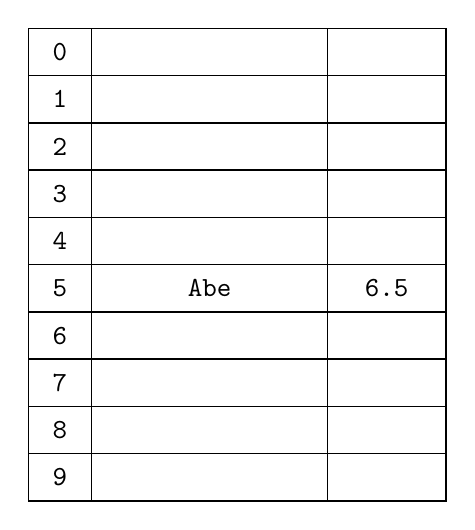
\begin{tikzpicture}

\draw (1.4, 0.7)
  node[draw, line width=0.02cm, , color=black,
       rounded corners=0cm, inner sep=0cm] {

\begin{minipage}[t][0.6cm]{0.8cm}
\mbox{}

\end{minipage}

};\draw (1.4, 0.7) node[color=black] {{\texttt{0}}};
\draw (3.3, 0.7)
  node[draw, line width=0.02cm, , color=black,
       rounded corners=0cm, inner sep=0cm] {

\begin{minipage}[t][0.6cm]{3.0cm}
\mbox{}

\end{minipage}

};\draw (3.3, 0.7) node[color=black] {{\texttt{}}};
\draw (5.55, 0.7)
  node[draw, line width=0.02cm, , color=black,
       rounded corners=0cm, inner sep=0cm] {

\begin{minipage}[t][0.6cm]{1.5cm}
\mbox{}

\end{minipage}

};\draw (5.55, 0.7) node[color=black] {{\texttt{}}};
\draw (1.4, 0.09999999999999987)
  node[draw, line width=0.02cm, , color=black,
       rounded corners=0cm, inner sep=0cm] {

\begin{minipage}[t][0.6cm]{0.8cm}
\mbox{}

\end{minipage}

};\draw (1.4, 0.09999999999999987) node[color=black] {{\texttt{1}}};
\draw (3.3, 0.09999999999999987)
  node[draw, line width=0.02cm, , color=black,
       rounded corners=0cm, inner sep=0cm] {

\begin{minipage}[t][0.6cm]{3.0cm}
\mbox{}

\end{minipage}

};\draw (3.3, 0.09999999999999987) node[color=black] {{\texttt{}}};
\draw (5.55, 0.09999999999999987)
  node[draw, line width=0.02cm, , color=black,
       rounded corners=0cm, inner sep=0cm] {

\begin{minipage}[t][0.6cm]{1.5cm}
\mbox{}

\end{minipage}

};\draw (5.55, 0.09999999999999987) node[color=black] {{\texttt{}}};
\draw (1.4, -0.5000000000000002)
  node[draw, line width=0.02cm, , color=black,
       rounded corners=0cm, inner sep=0cm] {

\begin{minipage}[t][0.6cm]{0.8cm}
\mbox{}

\end{minipage}

};\draw (1.4, -0.5000000000000002) node[color=black] {{\texttt{2}}};
\draw (3.3, -0.5000000000000002)
  node[draw, line width=0.02cm, , color=black,
       rounded corners=0cm, inner sep=0cm] {

\begin{minipage}[t][0.6cm]{3.0cm}
\mbox{}

\end{minipage}

};\draw (3.3, -0.5000000000000002) node[color=black] {{\texttt{}}};
\draw (5.55, -0.5000000000000002)
  node[draw, line width=0.02cm, , color=black,
       rounded corners=0cm, inner sep=0cm] {

\begin{minipage}[t][0.6cm]{1.5cm}
\mbox{}

\end{minipage}

};\draw (5.55, -0.5000000000000002) node[color=black] {{\texttt{}}};
\draw (1.4, -1.1000000000000003)
  node[draw, line width=0.02cm, , color=black,
       rounded corners=0cm, inner sep=0cm] {

\begin{minipage}[t][0.6cm]{0.8cm}
\mbox{}

\end{minipage}

};\draw (1.4, -1.1000000000000003) node[color=black] {{\texttt{3}}};
\draw (3.3, -1.1000000000000003)
  node[draw, line width=0.02cm, , color=black,
       rounded corners=0cm, inner sep=0cm] {

\begin{minipage}[t][0.6cm]{3.0cm}
\mbox{}

\end{minipage}

};\draw (3.3, -1.1000000000000003) node[color=black] {{\texttt{}}};
\draw (5.55, -1.1000000000000003)
  node[draw, line width=0.02cm, , color=black,
       rounded corners=0cm, inner sep=0cm] {

\begin{minipage}[t][0.6cm]{1.5cm}
\mbox{}

\end{minipage}

};\draw (5.55, -1.1000000000000003) node[color=black] {{\texttt{}}};
\draw (1.4, -1.7000000000000002)
  node[draw, line width=0.02cm, , color=black,
       rounded corners=0cm, inner sep=0cm] {

\begin{minipage}[t][0.6cm]{0.8cm}
\mbox{}

\end{minipage}

};\draw (1.4, -1.7000000000000002) node[color=black] {{\texttt{4}}};
\draw (3.3, -1.7000000000000002)
  node[draw, line width=0.02cm, , color=black,
       rounded corners=0cm, inner sep=0cm] {

\begin{minipage}[t][0.6cm]{3.0cm}
\mbox{}

\end{minipage}

};\draw (3.3, -1.7000000000000002) node[color=black] {{\texttt{}}};
\draw (5.55, -1.7000000000000002)
  node[draw, line width=0.02cm, , color=black,
       rounded corners=0cm, inner sep=0cm] {

\begin{minipage}[t][0.6cm]{1.5cm}
\mbox{}

\end{minipage}

};\draw (5.55, -1.7000000000000002) node[color=black] {{\texttt{}}};
\draw (1.4, -2.3000000000000003)
  node[draw, line width=0.02cm, , color=black,
       rounded corners=0cm, inner sep=0cm] {

\begin{minipage}[t][0.6cm]{0.8cm}
\mbox{}

\end{minipage}

};\draw (1.4, -2.3000000000000003) node[color=black] {{\texttt{5}}};
\draw (3.3, -2.3000000000000003)
  node[draw, line width=0.02cm, , color=black,
       rounded corners=0cm, inner sep=0cm] {

\begin{minipage}[t][0.6cm]{3.0cm}
\mbox{}

\end{minipage}

};\draw (3.3, -2.3000000000000003) node[color=black] {{\texttt{Abe}}};
\draw (5.55, -2.3000000000000003)
  node[draw, line width=0.02cm, , color=black,
       rounded corners=0cm, inner sep=0cm] {

\begin{minipage}[t][0.6cm]{1.5cm}
\mbox{}

\end{minipage}

};\draw (5.55, -2.3000000000000003) node[color=black] {{\texttt{6.5}}};
\draw (1.4, -2.9000000000000004)
  node[draw, line width=0.02cm, , color=black,
       rounded corners=0cm, inner sep=0cm] {

\begin{minipage}[t][0.6cm]{0.8cm}
\mbox{}

\end{minipage}

};\draw (1.4, -2.9000000000000004) node[color=black] {{\texttt{6}}};
\draw (3.3, -2.9000000000000004)
  node[draw, line width=0.02cm, , color=black,
       rounded corners=0cm, inner sep=0cm] {

\begin{minipage}[t][0.6cm]{3.0cm}
\mbox{}

\end{minipage}

};\draw (3.3, -2.9000000000000004) node[color=black] {{\texttt{}}};
\draw (5.55, -2.9000000000000004)
  node[draw, line width=0.02cm, , color=black,
       rounded corners=0cm, inner sep=0cm] {

\begin{minipage}[t][0.6cm]{1.5cm}
\mbox{}

\end{minipage}

};\draw (5.55, -2.9000000000000004) node[color=black] {{\texttt{}}};
\draw (1.4, -3.500000000000001)
  node[draw, line width=0.02cm, , color=black,
       rounded corners=0cm, inner sep=0cm] {

\begin{minipage}[t][0.6cm]{0.8cm}
\mbox{}

\end{minipage}

};\draw (1.4, -3.500000000000001) node[color=black] {{\texttt{7}}};
\draw (3.3, -3.500000000000001)
  node[draw, line width=0.02cm, , color=black,
       rounded corners=0cm, inner sep=0cm] {

\begin{minipage}[t][0.6cm]{3.0cm}
\mbox{}

\end{minipage}

};\draw (3.3, -3.500000000000001) node[color=black] {{\texttt{}}};
\draw (5.55, -3.500000000000001)
  node[draw, line width=0.02cm, , color=black,
       rounded corners=0cm, inner sep=0cm] {

\begin{minipage}[t][0.6cm]{1.5cm}
\mbox{}

\end{minipage}

};\draw (5.55, -3.500000000000001) node[color=black] {{\texttt{}}};
\draw (1.4, -4.1000000000000005)
  node[draw, line width=0.02cm, , color=black,
       rounded corners=0cm, inner sep=0cm] {

\begin{minipage}[t][0.6cm]{0.8cm}
\mbox{}

\end{minipage}

};\draw (1.4, -4.1000000000000005) node[color=black] {{\texttt{8}}};
\draw (3.3, -4.1000000000000005)
  node[draw, line width=0.02cm, , color=black,
       rounded corners=0cm, inner sep=0cm] {

\begin{minipage}[t][0.6cm]{3.0cm}
\mbox{}

\end{minipage}

};\draw (3.3, -4.1000000000000005) node[color=black] {{\texttt{}}};
\draw (5.55, -4.1000000000000005)
  node[draw, line width=0.02cm, , color=black,
       rounded corners=0cm, inner sep=0cm] {

\begin{minipage}[t][0.6cm]{1.5cm}
\mbox{}

\end{minipage}

};\draw (5.55, -4.1000000000000005) node[color=black] {{\texttt{}}};
\draw (1.4, -4.7)
  node[draw, line width=0.02cm, , color=black,
       rounded corners=0cm, inner sep=0cm] {

\begin{minipage}[t][0.6cm]{0.8cm}
\mbox{}

\end{minipage}

};\draw (1.4, -4.7) node[color=black] {{\texttt{9}}};
\draw (3.3, -4.7)
  node[draw, line width=0.02cm, , color=black,
       rounded corners=0cm, inner sep=0cm] {

\begin{minipage}[t][0.6cm]{3.0cm}
\mbox{}

\end{minipage}

};\draw (3.3, -4.7) node[color=black] {{\texttt{}}};
\draw (5.55, -4.7)
  node[draw, line width=0.02cm, , color=black,
       rounded corners=0cm, inner sep=0cm] {

\begin{minipage}[t][0.6cm]{1.5cm}
\mbox{}

\end{minipage}

};\draw (5.55, -4.7) node[color=black] {{\texttt{}}};
\end{tikzpicture}

\end{center}



%-*-latex-*-

\begin{ex} 
  \label{ex:prob-00}
  \tinysidebar{\debug{exercises/{disc-prob-28/question.tex}}}

  \solutionlink{sol:prob-00}
  \qed
\end{ex} 
\begin{python0}
from solutions import *
add(label="ex:prob-00",
    srcfilename='exercises/discrete-probability/prob-00/answer.tex') 
\end{python0}


Of course if your \verb!N! is really, really, really huge,
you will find that the probability of getting a head is 0.5 and 
the probability of getting a tail is 0.5.

Here's a function (derived by simulation) 
that gives us the probability for each possible outcome
of our experiment:
\includesourcenonumbers{tossfaircoin3.py}
I've increase \verb!n! to 1000 and 
also commented out the printing of each experiment.
Here's my output when I run the program:
\begin{center}
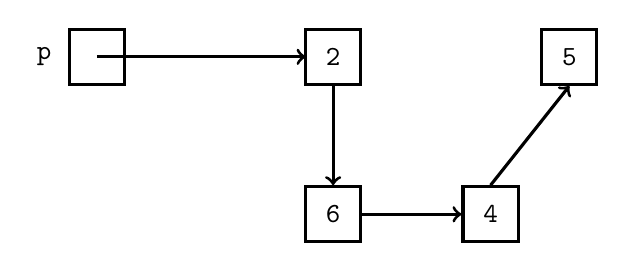
\begin{tikzpicture}

\draw (0.35, 0.35)
  node[draw, line width=0.04cm, , color=black,
       rounded corners=0cm, inner sep=0cm] {

\begin{minipage}[t][0.7cm]{0.7cm}
\mbox{}

\end{minipage}

};\draw (0.35, 0.35) node[color=black] {{\texttt{2}}};
\draw (0.35, -1.65)
  node[draw, line width=0.04cm, , color=black,
       rounded corners=0cm, inner sep=0cm] {

\begin{minipage}[t][0.7cm]{0.7cm}
\mbox{}

\end{minipage}

};\draw (0.35, -1.65) node[color=black] {{\texttt{6}}};
\draw (2.35, -1.65)
  node[draw, line width=0.04cm, , color=black,
       rounded corners=0cm, inner sep=0cm] {

\begin{minipage}[t][0.7cm]{0.7cm}
\mbox{}

\end{minipage}

};\draw (2.35, -1.65) node[color=black] {{\texttt{4}}};
\draw (3.35, 0.35)
  node[draw, line width=0.04cm, , color=black,
       rounded corners=0cm, inner sep=0cm] {

\begin{minipage}[t][0.7cm]{0.7cm}
\mbox{}

\end{minipage}

};\draw (3.35, 0.35) node[color=black] {{\texttt{5}}};\draw[line width=0.04cm,black,->] (0.35,-0.02) to  (0.35,-1.28);
\draw[line width=0.04cm,black,->] (0.72,-1.65) to  (1.98,-1.65);
\draw[line width=0.04cm,black,->] (2.35,-1.28) to  (3.35,-0.02);

\draw (-2.65, 0.35)
  node[draw, line width=0.04cm, , color=black,
       rounded corners=0cm, inner sep=0cm] {

\begin{minipage}[t][0.7cm]{0.7cm}
\mbox{}

\end{minipage}

};\draw (-2.65, 0.35) node[color=black] {{\texttt{}}};\draw[line width=0.04cm,black,->] (-2.65,0.35) to  (0,0.35);

\draw (-3.32, 0.35)
  node[draw, line width=0.04cm, , color=white,
       rounded corners=0cm, inner sep=0cm] {

\begin{minipage}[t][0.1cm]{0.1cm}
\mbox{}

\end{minipage}

};\draw (-3.32, 0.35) node[color=black] {{\texttt{p}}};
\end{tikzpicture}

\end{center}



Of course if we assume from the beginning that our coin is fair we can 
save the trouble of the computation:
\includesourcenonumbers{tossfaircoin4.py}
Here's my output when I run the program:
\begin{center}
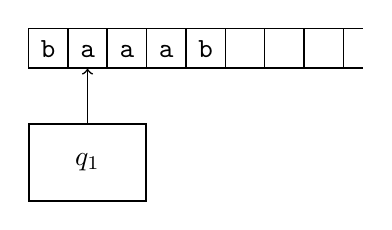
\begin{tikzpicture}

\draw (0.25, 0.25)
  node[draw, line width=0.02cm, , color=black,
       rounded corners=0cm, inner sep=0cm] {

\begin{minipage}[t][0.5cm]{0.5cm}
\mbox{}

\end{minipage}

};\draw (0.25, 0.25) node[color=black] {{\vphantom{baaab\SPACE\SPACE\SPACE}\texttt{b}}};
\draw (0.75, 0.25)
  node[draw, line width=0.02cm, , color=black,
       rounded corners=0cm, inner sep=0cm] {

\begin{minipage}[t][0.5cm]{0.5cm}
\mbox{}

\end{minipage}

};\draw (0.75, 0.25) node[color=black] {{\vphantom{baaab\SPACE\SPACE\SPACE}\texttt{a}}};
\draw (1.25, 0.25)
  node[draw, line width=0.02cm, , color=black,
       rounded corners=0cm, inner sep=0cm] {

\begin{minipage}[t][0.5cm]{0.5cm}
\mbox{}

\end{minipage}

};\draw (1.25, 0.25) node[color=black] {{\vphantom{baaab\SPACE\SPACE\SPACE}\texttt{a}}};
\draw (1.75, 0.25)
  node[draw, line width=0.02cm, , color=black,
       rounded corners=0cm, inner sep=0cm] {

\begin{minipage}[t][0.5cm]{0.5cm}
\mbox{}

\end{minipage}

};\draw (1.75, 0.25) node[color=black] {{\vphantom{baaab\SPACE\SPACE\SPACE}\texttt{a}}};
\draw (2.25, 0.25)
  node[draw, line width=0.02cm, , color=black,
       rounded corners=0cm, inner sep=0cm] {

\begin{minipage}[t][0.5cm]{0.5cm}
\mbox{}

\end{minipage}

};\draw (2.25, 0.25) node[color=black] {{\vphantom{baaab\SPACE\SPACE\SPACE}\texttt{b}}};
\draw (2.75, 0.25)
  node[draw, line width=0.02cm, , color=black,
       rounded corners=0cm, inner sep=0cm] {

\begin{minipage}[t][0.5cm]{0.5cm}
\mbox{}

\end{minipage}

};\draw (2.75, 0.25) node[color=black] {{\vphantom{baaab\SPACE\SPACE\SPACE}\texttt{\SPACE}}};
\draw (3.25, 0.25)
  node[draw, line width=0.02cm, , color=black,
       rounded corners=0cm, inner sep=0cm] {

\begin{minipage}[t][0.5cm]{0.5cm}
\mbox{}

\end{minipage}

};\draw (3.25, 0.25) node[color=black] {{\vphantom{baaab\SPACE\SPACE\SPACE}\texttt{\SPACE}}};
\draw (3.75, 0.25)
  node[draw, line width=0.02cm, , color=black,
       rounded corners=0cm, inner sep=0cm] {

\begin{minipage}[t][0.5cm]{0.5cm}
\mbox{}

\end{minipage}

};\draw (3.75, 0.25) node[color=black] {{\vphantom{baaab\SPACE\SPACE\SPACE}\texttt{\SPACE}}};\draw[line width=0.02cm,black] (4.0,0.5) to  (4.25,0.5);
\draw[line width=0.02cm,black] (4.0,0.0) to  (4.25,0.0);

\draw (0.75, -1.2)
  node[draw, line width=0.02cm, , color=black,
       rounded corners=0cm, inner sep=0cm] {

\begin{minipage}[t][0.98cm]{1.48cm}
\mbox{}

\end{minipage}

};\draw (0.75, -1.2) node[color=black] {$q_1$};\draw[line width=0.02cm,black,->] (0.75,-0.7) to  (0.75,-0.47) to  (0.75,-0.47) to  (0.75,-0.01);
\end{tikzpicture}

\end{center}



Of course when \verb!n! gets larger and larger, the probability function
derived using simulations will match this new \lq\lq theoretically'' derived
function.

%-*-latex-*-

\begin{ex} 
  \label{ex:prob-00}
  \tinysidebar{\debug{exercises/{disc-prob-28/question.tex}}}

  \solutionlink{sol:prob-00}
  \qed
\end{ex} 
\begin{python0}
from solutions import *
add(label="ex:prob-00",
    srcfilename='exercises/discrete-probability/prob-00/answer.tex') 
\end{python0}

%-*-latex-*-

\begin{ex} 
  \label{ex:prob-00}
  \tinysidebar{\debug{exercises/{disc-prob-28/question.tex}}}

  \solutionlink{sol:prob-00}
  \qed
\end{ex} 
\begin{python0}
from solutions import *
add(label="ex:prob-00",
    srcfilename='exercises/discrete-probability/prob-00/answer.tex') 
\end{python0}

%-*-latex-*-

\begin{ex} 
  \label{ex:prob-00}
  \tinysidebar{\debug{exercises/{disc-prob-28/question.tex}}}

  \solutionlink{sol:prob-00}
  \qed
\end{ex} 
\begin{python0}
from solutions import *
add(label="ex:prob-00",
    srcfilename='exercises/discrete-probability/prob-00/answer.tex') 
\end{python0}


I abstract the coin toss experiment as follows:
Let $S = \{\HEAD, \TAIL\}$ represent all possible outcomes of
my coin toss experiment.
$S$ is the called the \defone{sample space} of my random experiment.
$\HEAD$ and $\TAIL$ are called
the \defone{outcomes} of my experiment.
I define a function
\[
  p : S \rightarrow \R 
\]
such that $p(\HEAD)$ gives us the chance that
a coin toss will give us a head and
$p(\TAIL)$ gives us the chance of getting a tail.
So if the coin is fair, I would have
\[
  p(\HEAD) = 1/2 = p(\TAIL)
\]
$p$ is called a
\defterm{probability distribution function}\index{probability distribution function}\tinysidebar{probability distribution function \\ pdf}
(\defterm{pdf}\index{pdf}):
it distributes $1$ to all outcomes:
\[
1 = p(\HEAD) + p(\TAIL) = \sum_{x \in S} p(x)
\]
$p$ is also called a
\defterm{probability function}\index{probability function}\tinysidebar{probability function \\ probability mass function}
or a 
\defterm{probability mass function}\index{probability mass function}.




\newpage
\subsection{Die rolls}

When you roll a die, you get the face value of the roll, i.e.,
the number of dots on the top surface of the die, you
get one of the following:
\[
\text{
\texttt{ONE},
\texttt{TWO},
\texttt{THREE},
\texttt{FOUR},
\texttt{FIVE},
\texttt{SIX},
}
\]
Assuming that the die is fair and you roll the die a huge
number of times, you will see that approximately 1/6 of the 
rolls will give you a \texttt{ONE}
(and likewise for the other cases.)

I can assign 1/6 to \texttt{ONE} to indicate that the 
proportion of rolls that gives me \texttt{ONE}.
Likewise for the other cases.
This is basically a function
\[
p : \{\texttt{ONE},
\texttt{TWO},
\texttt{THREE},
\texttt{FOUR},
\texttt{FIVE},
\texttt{SIX}
\}
\rightarrow [0,1]
\]
such that 
\begin{align*}
p(\texttt{ONE}) &= 1/6 \\
p(\texttt{TWO}) &= 1/6 \\
p(\texttt{THREE}) &= 1/6 \\
p(\texttt{FOUR}) &= 1/6 \\
p(\texttt{FIVE}) &= 1/6 \\
p(\texttt{SIX}) &= 1/6
\end{align*}
As in the previous subsection, the set 
$S = \{
\texttt{ONE},
\texttt{TWO},
\texttt{THREE},
\texttt{FOUR},
\texttt{FIVE},
\texttt{SIX}
\}$ 
is called the set of outcomes or the sample space
of my experiment of rolling a die.
Note that
\[
\sum_{x \in S} p(x) = 1
\]

For us, our sample space is a finite set (you can also 
talk about probability theory for non-finite sets.) 


%-*-latex-*-

\begin{ex} 
  \label{ex:prob-00}
  \tinysidebar{\debug{exercises/{disc-prob-28/question.tex}}}

  \solutionlink{sol:prob-00}
  \qed
\end{ex} 
\begin{python0}
from solutions import *
add(label="ex:prob-00",
    srcfilename='exercises/discrete-probability/prob-00/answer.tex') 
\end{python0}

%-*-latex-*-

\begin{ex} 
  \label{ex:prob-00}
  \tinysidebar{\debug{exercises/{disc-prob-28/question.tex}}}

  \solutionlink{sol:prob-00}
  \qed
\end{ex} 
\begin{python0}
from solutions import *
add(label="ex:prob-00",
    srcfilename='exercises/discrete-probability/prob-00/answer.tex') 
\end{python0}


A probability distribution function is \defone{uniform}
if $p(x)$ is the same for all $x$ in the sample space of the function.
When I say that I'm rolling a \defone{fair} die, I mean that the probability
function for the experiment (of rolling the die) is uniform.

%-*-latex-*-

\begin{ex} 
  \label{ex:prob-00}
  \tinysidebar{\debug{exercises/{disc-prob-28/question.tex}}}

  \solutionlink{sol:prob-00}
  \qed
\end{ex} 
\begin{python0}
from solutions import *
add(label="ex:prob-00",
    srcfilename='exercises/discrete-probability/prob-00/answer.tex') 
\end{python0}


Instead of asking the probability of getting a \texttt{SIX} when
I roll a die, I might be interested in getting \texttt{ONE} or \texttt{SIX}.
In general, a subset $A$ of the set of all outcomes is called an 
\defone{event}.
In that case, I will write $p(A)$ or $p[A]$ for
\[
p(A) = \sum_{x \in A} p(x)
\]
So for instance in the case of our die,
\[
p[\{\texttt{ONE}, \texttt{SIX}\}]
= p(\texttt{ONE}) + p(\texttt{SIX})
= 1/6 + 1/6 = 1/3
\]

Let $A$ and $B$ be events of an experiment with sample space $S$
and probability distribution function $p$.
Then
\[
p[A \cup B] \leq p[A] + p[B]
\]
This means that if we know a lot about the probability of $A$ and 
probability of $B$, but we're not very sure about the common
events of $A$ and $B$, we can still bound the probability of $A \cup B$.
If we do know something about the probability of $A \cap B$, then we have
\[
p[A \cup B] = p[A] + p[B] - p[A \cap B]
\]

If $A \cap B = \emptyset$, we get
\[
p[A \cup B] = p[A] + p[B]
\]
Clearly we also have
\[
p[\emptyset] = 0
\]
and
\[
p[S] = 1
\]

Clearly
\[
p[\overline{A}] = 1 - p[A]
\]
where $\overline{A} = S - A$ is the complement of $A$ (with respect to $S$).

\newpage%-*-latex-*-
\sectionthree{Experimental (or Empirical) Approach}
\begin{python0}
from solutions import *; clear()
\end{python0}

Here's how to think of probability intuitively:
You can of course think of probability as some kind of averaging.
In the case of tossing a particular coin, if you say
\[
p(\HEAD) = \frac{1}{3}
\]
what you meant is that if you toss the coin 3 times, then
it's likely that 
approximately 1 out of the 3 is a head;
if you toss the coin 300 times, then it's very likely that
approximately 100 of the 300 are heads;
if you toss the coin 3000 times, then it's very very likely that
approximately 1000 of the 3000 are heads; etc.
The more tosses you make, the closer you get to \lq\lq one third of the
tosses comes out head''.

In the above coin toss experiment, I have two possible outcomes:
either I get a head or I get a tail.
I create two symbols to represent these two possible outcomes:
$\HEAD$ and $\TAIL$.
The names is arbitrary and it's entirely up to you to come up with
symbols for all the possible outcomes.
For instance you can name the outcomes H and T instead of
$\HEAD$ and $\TAIL$.

How let's formalize the notation for studying probability theory ...


\newpage%-*-latex-*-
\section{Probability distribution function}

A (finite) discrete 
\defone{probability distribution function} is
a 
real-valued function on a finite set $S$ 
\[
p : S \rightarrow \R
\]
such that 
\begin{axioms}
\item[{[DP-1]}] $0 \leq p(x) \leq 1$ for all $x \in S$
\item[{[DP-2]}] $\sum_{x \in S} p(x) = 1$
\end{axioms}
$S$ is a
\defterm{sample space}\index{sample space}\tinysidebar{sample space \\ outcomes}.
The elements of $S$ are called
\defterm{outcomes}\index{outcomes},
Because of [DP-1], I can change the codmain of $p$:
\[
p : S \rightarrow [0,1]
\]
A subset of $S$ is called an \defone{event}.
If $A$ is a subset of $S$, I'll write
\[
p(A) = \sum_{x \in A} p(x)
\]
[DP-2] is the same as saying
\[
p(S) = 1
\]

Here are some basic facts about pdfs.


%-*-latex-*-

\begin{ex} 
  \label{ex:prob-00}
  \tinysidebar{\debug{exercises/{disc-prob-28/question.tex}}}

  \solutionlink{sol:prob-00}
  \qed
\end{ex} 
\begin{python0}
from solutions import *
add(label="ex:prob-00",
    srcfilename='exercises/discrete-probability/prob-00/answer.tex') 
\end{python0}



\begin{defn}
A probability distribution function $p : S \rightarrow [0,1]$ 
is said to be \defone{uniform} if
\[
p(x) = \frac{1}{|S|}
\]
for each $x \in S$.
$|S|$, the size of $S$, denotes the numbers of distinct elements in $S$.
\end{defn}

\begin{eg}
Suppose that I've rigged my coin so that the chance of getting
a head is twice of getting the tail.
This means that the probability function
\[
p : S \rightarrow [0,1]
\]
is
\[
p(\HEAD) = \frac{2}{3}, \,\,\,\,\,
p(\TAIL) = \frac{1}{3} \,\,\,\,\,
\]
Of course if the coin is a fair coin I would have
\[
p(\HEAD) = \frac{1}{2} = p(\TAIL)
\]
\qed
\end{eg}


%-*-latex-*-

\begin{ex} 
  \label{ex:prob-00}
  \tinysidebar{\debug{exercises/{disc-prob-28/question.tex}}}

  \solutionlink{sol:prob-00}
  \qed
\end{ex} 
\begin{python0}
from solutions import *
add(label="ex:prob-00",
    srcfilename='exercises/discrete-probability/prob-00/answer.tex') 
\end{python0}



\begin{eg}
Suppose I have a loaded die such that getting a \lq\lq 1'' 
is 10 times more likely 
than the others and the others are equally likely.
Let $p$ be the probability function of rolling this die.
Then
\begin{align*}
1 
&= p(\ONE) + p(\TWO) + \cdots + p(\SIX) \\
&= p(\ONE) + 5 \cdot p(\TWO) \\
&= p(\ONE) + 5 \cdot \frac{1}{10} p(\ONE) \\
&= \frac{3}{2} \cdot p(\ONE) 
\end{align*}
So 
\[
p(\ONE) = \frac{2}{3}
\]
and 
\[
p(\TWO) = p(\THREE) = ... = p(\SIX) = \frac{2}{30}
\]
And of course
\[
S = \{\ONE, \TWO, \THREE, \FOUR, \FIVE, \SIX\}
\]

Go ahead and write a program to simulate tossing my loaded die.
Run it for a large number of experiments and check that you get the
expected results. 
\begin{Verbatim}[fontsize=\small, frame=single]
import random; random.seed()

ONE = "ONE"
TWO = "TWO"
THREE = "THREE"
FOUR = "FOUR"
FIVE = "FIVE"
SIX = "SIX"

# write a probability function for this experiment

def roll_die():
    r = random.randrange(30)
    if r < 20: return ONE
    elif r < 22: return TWO
    elif r < 24: return THREE
    elif r < 26: return FOUR
    elif r < 28: return FIVE
    else: return SIX

NUM_EXPERIMENTS = 20
for i in range(NUM_EXPERIMENTS):
    print("experiment", i, "... outcome:", roll_die())
\end{Verbatim}
\end{eg}


The following function can be used to produce the different
experiment functions (you should type it up and run it ... if you're
too lazy to do that you can also grab the code from
our class web site ... look for \lq\lq probability library"):
\begin{Verbatim}[frame=single, fontsize=\small]
def build_experiment(xs):
    total = sum([b for (a,b) in xs])
    accumulate = xs[0]
    for (a,b) in xs[1:]:
        accumulate.append((a, accumulate[-1][1] + b)
    def experiment():
        r = random.randrange(total)
        for (a,b) in accumulate:
            if r < b: return a
        raise ValueError("r:%s greater than total:%s" %\
                         (r, total))
    return experiment

HEAD = "HEAD"
TAIL = "TAIL"
toss_coin = build_experiment([(HEAD, 2),
                              (TAIL, 1),
                             ])
ONE = "ONE"
TWO = "TWO"
THREE = "THREE"
FOUR = "FOUR"
FIVE = "FIVE"
SIX = "SIX"
roll_die = build_experiment([(ONE, 20),
                             (TWO, 2),
                             (THREE, 2),
                             (FOUR, 2),
                             (FIVE, 2),
                             (SIX, 2),
                            ])
\end{Verbatim}

%-*-latex-*-

\begin{ex} 
  \label{ex:prob-00}
  \tinysidebar{\debug{exercises/{disc-prob-28/question.tex}}}

  \solutionlink{sol:prob-00}
  \qed
\end{ex} 
\begin{python0}
from solutions import *
add(label="ex:prob-00",
    srcfilename='exercises/discrete-probability/prob-00/answer.tex') 
\end{python0}

%-*-latex-*-

\begin{ex} 
  \label{ex:prob-00}
  \tinysidebar{\debug{exercises/{disc-prob-28/question.tex}}}

  \solutionlink{sol:prob-00}
  \qed
\end{ex} 
\begin{python0}
from solutions import *
add(label="ex:prob-00",
    srcfilename='exercises/discrete-probability/prob-00/answer.tex') 
\end{python0}


Now what is asked is actually related to another
experiment: 
\lq\lq Attend 3 classes in a row''.
(Later you'll see how to view this as a \lq\lq product of
experiments''.)
There are two ways to compute an approximation of the desired
probability.

FIRST METHOD:
You should use the first experiment to generate a sequence of
$\mathsc{Q}$'s and
$\mathsc{N}$'s:
\[
\mathsc{Q},
\mathsc{Q},
\mathsc{N},
\mathsc{Q},
\mathsc{Q},
\mathsc{Q},
\mathsc{Q},
\mathsc{Q},
\mathsc{Q},
\mathsc{N},
\mathsc{Q},
\mathsc{Q},
...
\]
satisfying the given probability that
$p(\mathsc{Q}) = 0.8$ and
$p(\mathsc{N}) = 0.2$.
Next you look at all the consecutive triples.
For instance the above gives
\[
\mathsc{QQN},
\mathsc{QNQ},
\mathsc{NQQ},
\mathsc{QQQ},
\mathsc{QQQ},
\mathsc{QQQ},
\mathsc{QQQ},
\mathsc{QQQ},
\mathsc{QQN},
\mathsc{QNQ},
\mathsc{NQQ}, ...
\]
and then compute the approximate probability of seeing
$\mathsc{QQQ}$ in 
this sampling.
Of course you need to have a reasonbly huge sample.
You can either do this by hand or write a program to simulate the
experiment.

SECOND METHOD:
If you have a function for the first experiment, say
\verb!attend_class! which gives you $\mathsc{Q}$ or
$\mathsc{N}$, then you should have a
function say \verb!attend_3_classes! that uses \verb!attend_class!:
\begin{Verbatim}[frame=single]
Q = 'Q'
N = 'N'

def attend_3_classes():
    return [attend_class(), 
            attend_class(), 
            attend_class(),
           ]
\end{Verbatim}
Of course you can now generate samples and count:
\begin{Verbatim}[frame=single]
MAX = 100000
count = 0
for i in range(MAX):
    if attend_3_classes() == [Q, Q, Q]: 
        count += 1
print(float(count) / MAX)
\end{Verbatim}

%-*-latex-*-

\begin{ex} 
  \label{ex:prob-00}
  \tinysidebar{\debug{exercises/{disc-prob-28/question.tex}}}

  \solutionlink{sol:prob-00}
  \qed
\end{ex} 
\begin{python0}
from solutions import *
add(label="ex:prob-00",
    srcfilename='exercises/discrete-probability/prob-00/answer.tex') 
\end{python0}


\newpage%-*-latex-*-
\sectionthree{Random variable}
\begin{python0}
from solutions import *; clear()
\end{python0}

Now for the definition of a very confusing term: random variable.
A \defone{random variable} $X$ of $S$ (a sample space) is just a function
from $S$ to some set, say $V$.
\[
  X : S \rightarrow V
\]
Usually $V$ is the set of real numbers:
\[
  X : S \rightarrow \R
\]
It's really important to remember that a random variable
is not random and is not a variable!!!
It's just a function from a sample space to a set.
This is an example of a badly chosen name for this idea.

There are two main reasons why we need the concept of random variables.
Pay attention to the following.



\newpage
\subsection{Random variable as labels}

The first reason for having random variables is
that we want to create some 
labels for the values in a sample space.
The labels will then create subsets of the sample space, i.e.,
random variables helps create meaningful events.

As an example, I'm going back to the die roll experiment.
The sample space is
\[
S = \{\ONE, \TWO, \THREE, \FOUR, \FIVE, \SIX \}
\]
Suppose I'm playing a game with a die and I win
if the roll gives me either $\ONE$ or $\SIX$;
otherwise I lose.
I can then define the following
random variables:
\[
  X : \{ \ONE, ..., \SIX \} \rightarrow \{ \GOOD, \BAD \}
\]
where
\begin{align*}
  X(\ONE) &= X(\SIX) = \textsc{Good} \\
  X(\TWO) &= X(\THREE) = X(\FOUR) = X(\FIVE) = \BAD 
\end{align*}
We have create two subsets
\begin{align*}
  A &= \{ s \in S \mid X(s) = \GOOD \} \\
  B &= \{ s \in S \mid X(s) = \BAD \}
\end{align*}
of $S$.
In other words, random variables create events for each
value in the range of the random variables.
In fact the subsets created are disjoint
and the union of all these subsets for the original
sample space.
In other words, $X$ creates a partition of the sample space,
i.e., $A$ and $B$ are disjoint and $A \cup B$ is $X$.

As a consequence, my random variable $X$ also defines a new
probability distribution function
\[
  p_X : \{ \GOOD, \BAD \} \rightarrow [0,1]
\]
where
\begin{align*}
  p_X(\GOOD) &= p(\{ s \in S \mid X(s) = \GOOD \}) = 1/3 \\
  p_X(\BAD) &= p(\{ s \in S \mid X(s) = \BAD \}) = 2/3
\end{align*}
This function is very frequently written like this:
\begin{align*}
  \Pr[X = \GOOD] &= 1/3 \\
  \Pr[X = \BAD] &= 2/3
\end{align*}
or sometimes
$\operatorname{P}[X=\GOOD]$
or
$\operatorname{P}(X=\GOOD)$.
This $\Pr$ is a bad notation because this function
actually depends on $p$ and $X$.
But nobody write $\Pr_p[X = \GOOD]$.
Part of the reason is because a random variable $X$
is usually tied to a probability distribution function.
Which is not exactly true since $X$ is a function of
the sample space and is therefore tied to the sample space
and not the probability function itself.
But this is the practice and you have to remember what I said
above in order not to be confused.

It's important to note that $p_X$ and $\Pr[X= \bullet]$ are pdfs,
but they are \textit{not} pdf on $S$: they are pdfs on
$\{ \GOOD, \BAD \}$.

Here's a picture to keep in mind:
%-*-latex-*-
\begin{center}
\begin{tikzpicture}

\draw (0.625, 0.25)
  node[draw=none, line width=0cm, , color=black,
       rounded corners=0cm, inner sep=0cm,
       name=1] {

\begin{minipage}[t][0.5cm]{1.25cm}
\mbox{}

\end{minipage}

};\draw (0.625, 0.25) node[color=black] {$\ONE$};
\draw (0.625, -0.25)
  node[draw=none, line width=0cm, , color=black,
       rounded corners=0cm, inner sep=0cm,
       name=2] {

\begin{minipage}[t][0.5cm]{1.25cm}
\mbox{}

\end{minipage}

};\draw (0.625, -0.25) node[color=black] {$\TWO$};
\draw (0.625, -0.75)
  node[draw=none, line width=0cm, , color=black,
       rounded corners=0cm, inner sep=0cm,
       name=3] {

\begin{minipage}[t][0.5cm]{1.25cm}
\mbox{}

\end{minipage}

};\draw (0.625, -0.75) node[color=black] {$\THREE$};
\draw (0.625, -1.25)
  node[draw=none, line width=0cm, , color=black,
       rounded corners=0cm, inner sep=0cm,
       name=4] {

\begin{minipage}[t][0.5cm]{1.25cm}
\mbox{}

\end{minipage}

};\draw (0.625, -1.25) node[color=black] {$\FOUR$};
\draw (0.625, -1.75)
  node[draw=none, line width=0cm, , color=black,
       rounded corners=0cm, inner sep=0cm,
       name=5] {

\begin{minipage}[t][0.5cm]{1.25cm}
\mbox{}

\end{minipage}

};\draw (0.625, -1.75) node[color=black] {$\FIVE$};
\draw (0.625, -2.25)
  node[draw=none, line width=0cm, , color=black,
       rounded corners=0cm, inner sep=0cm,
       name=6] {

\begin{minipage}[t][0.5cm]{1.25cm}
\mbox{}

\end{minipage}

};\draw (0.625, -2.25) node[color=black] {$\SIX$};
\draw (4.5, -1.0)
  node[draw=none, line width=0cm, , color=black,
       rounded corners=0cm, inner sep=0cm,
       name=p] {

\begin{minipage}[t][0.5cm]{1cm}
\mbox{}

\end{minipage}

};\draw (4.5, -1.0) node[color=black] {$1/6$};\node [ellipse, draw=black, fit=(1) (2) (3) (4) (5) (6), line width=0.05cm, inner sep=0.0cm] {};\node [ellipse, draw=black, fit=(p), line width=0.05cm, inner sep=0.5cm] {};\draw[line width=0.04cm,black,->] (1) to  (p);
\draw[line width=0.04cm,black,->] (2) to  (p);
\draw[line width=0.04cm,black,->] (3) to  (p);
\draw[line width=0.04cm,black,->] (4) to  (p);
\draw[line width=0.04cm,black,->] (5) to  (p);
\draw[line width=0.04cm,black,->] (6) to  (p);

\draw (0.625, -3.75)
  node[draw=none, line width=0cm, , color=black,
       rounded corners=0cm, inner sep=0cm,
       name=g] {

\begin{minipage}[t][0.5cm]{1.25cm}
\mbox{}

\end{minipage}

};\draw (0.625, -3.75) node[color=black] {\textsc{\textblue{Good}}};
\draw (0.625, -4.25)
  node[draw=none, line width=0cm, , color=black,
       rounded corners=0cm, inner sep=0cm,
       name=b] {

\begin{minipage}[t][0.5cm]{1.25cm}
\mbox{}

\end{minipage}

};\draw (0.625, -4.25) node[color=black] {\textsc{\textred{Bad}}};\node [ellipse, draw=black, fit=(g) (b), line width=0.05cm, inner sep=0.0cm] {};
\draw (4.5, -3.75)
  node[draw=none, line width=0cm, , color=black,
       rounded corners=0cm, inner sep=0cm,
       name=13] {

\begin{minipage}[t][0.5cm]{1cm}
\mbox{}

\end{minipage}

};\draw (4.5, -3.75) node[color=black] {\textblue{$1/3$}};
\draw (4.5, -4.25)
  node[draw=none, line width=0cm, , color=black,
       rounded corners=0cm, inner sep=0cm,
       name=23] {

\begin{minipage}[t][0.5cm]{1cm}
\mbox{}

\end{minipage}

};\draw (4.5, -4.25) node[color=black] {\textred{$2/3$}};\node [ellipse, draw=black, fit=(13) (23), line width=0.05cm, inner sep=0.4cm] {};\draw[line width=0.04cm,blue,->] (g) to  (13);
\draw[line width=0.04cm,red,->] (b) to  (23);
\draw[line width=0.04cm,blue,->] (1) to [bend right=90]  (g);
\draw[line width=0.04cm,red,->] (2) to [bend right=90]  (b);
\draw[line width=0.04cm,red,->] (3) to [bend right=90]  (b);
\draw[line width=0.04cm,red,->] (4) to [bend right=90]  (b);
\draw[line width=0.04cm,red,->] (5) to [bend right=90]  (b);
\draw[line width=0.04cm,blue,->] (6) to [bend right=90]  (g);
\end{tikzpicture}

\end{center}



The function at the top is $p$ and the function
at the bottom is $\Pr[X = \bullet]$.
You can (and should) think of a random variable as
collecting probabilities given by $p$ into buckets.
You can think of it this way:

\begin{center}
\begin{tikzpicture}

\draw (0.625, 0.5)
  node[draw=none, line width=0cm, , color=black,
       rounded corners=0cm, inner sep=0cm,
       name=1] {

\begin{minipage}[t][1.0cm]{1.25cm}
\mbox{}

\end{minipage}

};\draw (0.625, 0.5) node[color=black] {$\ONE$};
\draw (0.625, 0.0)
  node[draw=none, line width=0cm, , color=black,
       rounded corners=0cm, inner sep=0cm,
       name=6] {

\begin{minipage}[t][1.0cm]{1.25cm}
\mbox{}

\end{minipage}

};\draw (0.625, 0.0) node[color=black] {$\SIX$};
\draw (0.625, -2.2)
  node[draw=none, line width=0cm, , color=black,
       rounded corners=0cm, inner sep=0cm,
       name=2] {

\begin{minipage}[t][1.0cm]{1.25cm}
\mbox{}

\end{minipage}

};\draw (0.625, -2.2) node[color=black] {$\TWO$};
\draw (0.625, -2.7)
  node[draw=none, line width=0cm, , color=black,
       rounded corners=0cm, inner sep=0cm,
       name=3] {

\begin{minipage}[t][1.0cm]{1.25cm}
\mbox{}

\end{minipage}

};\draw (0.625, -2.7) node[color=black] {$\THREE$};
\draw (0.625, -3.2)
  node[draw=none, line width=0cm, , color=black,
       rounded corners=0cm, inner sep=0cm,
       name=4] {

\begin{minipage}[t][1.0cm]{1.25cm}
\mbox{}

\end{minipage}

};\draw (0.625, -3.2) node[color=black] {$\FOUR$};
\draw (0.625, -3.7)
  node[draw=none, line width=0cm, , color=black,
       rounded corners=0cm, inner sep=0cm,
       name=5] {

\begin{minipage}[t][1.0cm]{1.25cm}
\mbox{}

\end{minipage}

};\draw (0.625, -3.7) node[color=black] {$\FIVE$};
\draw (4.5, 0.0)
  node[draw=none, line width=0cm, , color=black,
       rounded corners=0cm, inner sep=0cm,
       name=p] {

\begin{minipage}[t][0.5cm]{1cm}
\mbox{}

\end{minipage}

};\draw (4.5, 0.0) node[color=black] {$1/6$};\node [ellipse, draw=blue, fit=(1) (6), line width=0.05cm, inner sep=0.1cm] (good) {};\node [ellipse, draw=red, fit=(2) (3) (4) (5), line width=0.05cm, inner sep=0.1cm] (bad) {};\node [ellipse, draw=black, fit=(good) (bad), line width=0.05cm, inner sep=0.1cm] {};\node [ellipse, draw=black, fit=(p), line width=0.05cm, inner sep=0.5cm] {};\draw[line width=0.04cm,black,->] (1) to  (p);
\draw[line width=0.04cm,black,->] (2) to  (p);
\draw[line width=0.04cm,black,->] (3) to  (p);
\draw[line width=0.04cm,black,->] (4) to  (p);
\draw[line width=0.04cm,black,->] (5) to  (p);
\draw[line width=0.04cm,black,->] (6) to  (p);

\draw (4.5, -2.75)
  node[draw=none, line width=0cm, , color=black,
       rounded corners=0cm, inner sep=0cm,
       name=13] {

\begin{minipage}[t][0.5cm]{1cm}
\mbox{}

\end{minipage}

};\draw (4.5, -2.75) node[color=black] {\textblue{$1/3$}};
\draw (4.5, -3.25)
  node[draw=none, line width=0cm, , color=black,
       rounded corners=0cm, inner sep=0cm,
       name=23] {

\begin{minipage}[t][0.5cm]{1cm}
\mbox{}

\end{minipage}

};\draw (4.5, -3.25) node[color=black] {\textred{$2/3$}};\node [ellipse, draw=black, fit=(13) (23), line width=0.05cm, inner sep=0.4cm] {};\draw[line width=0.04cm,blue,->] (good) to  (13);
\draw[line width=0.04cm,red,->] (bad) to  (23);
\end{tikzpicture}

\end{center}



The random variable $X$ basically collects up probabilities:
$\ONE$ and $\SIX$ are collected up into \GOOD\
and the rest are collected up into \BAD.

It's possible, in fact it's common, to have multiple
random variables on the same sample space.

Here's another random variable:
\[
Y : S \rightarrow \{ \EVEN, \ODD \}
\]
where
\begin{align*}
Y(\ONE) &= Y(\THREE) = Y(\FIVE) = \ODD \\
Y(\TWO) &= Y(\FOUR) = Y(\SIX) = \EVEN
\end{align*}
This means that we can talk about
\[
\Pr[Y = \ODD]
\]
which of course is just
\[
p(\{s \in S \mid Y(s) = \ODD \})
\]
Our $Y$ allows us to create the following subsets of $S$:
\begin{myenum}
  \li $\{ x \in S \mid Y(x) = \EVEN \} = \{\TWO, \FOUR, \SIX \} \subseteq S$
  \li $\{ x \in S \mid Y(x) = \ODD \} = \{\ONE, \THREE, \FIVE \} \subseteq S$
\end{myenum}
This $Y$ creates a pdf
\[
  \Pr[Y = \bullet] : \{ \EVEN, \ODD \} \rightarrow [0, 1]
\]
where
\[
  \Pr[Y = \EVEN] = \Pr[Y = \ODD] = \frac{1}{2}
\]

Here's yet another random variable on die rolls:
\[
Z : S \rightarrow \{ \textsc{Small}, \textsc{Medium}, \textsc{Large} \}
\]
where
\begin{align*}
Z(\ONE) &= Z(\TWO) = \textsc{Small} \\
Z(\THREE) &= Z(\FOUR) = \textsc{Medium} \\
Z(\FIVE) &= Z(\SIX) = \textsc{Large}
\end{align*}

Frequently instead of just
\[
  \Pr[Z = \textsc{Small}]
\]
you actually see expressions like this:
\[
  \Pr[Z = \textsc{Small} \text{ or } Z = \textsc{Medium}]
\]
or more formally
\[
  \Pr[Z \in \{\textsc{Small}, \textsc{Medium}\}]
\]
In other words
\[
  \Pr[\text{boolean expression on a random variable}]  
\]
and even boolean expressions involving more than one random variables:
\[
\Pr[Y = \ODD \lor Z = \text{Small}]  
\]
In this case
\[
\Pr[Y = \ODD \ \lor \ Z = \text{Small}]
=
\sum_{\stackrel{s \in S}{Y(s) = \ODD \ \lor \ Z(s) = \text{Small}}} p(s)
\]


Here's another random variable where the value of the random variable
takes a real values.
For instance, for the die rolling experiment, suppose I define $W$
in the obvious way:
\begin{align*}
W(\ONE) &= 1 \\
W(\TWO) &= 2 \\
W(\THREE) &= 3 \\
W(\FOUR) &= 4 \\
W(\FIVE) &= 5 \\
W(\SIX) &= 6 \\
\end{align*}
With this random variable $W$, I can write
\[
\Pr[W \text{ is odd}]
\]
to mean
$\Pr[W \in \{\ONE, \THREE, \FIVE\}]$.
I can even write
$\Pr[W \leq 4]$.
The meaning should be obvious.

In general, suppose $p : S \rightarrow \R$ is a probability distribution function
and $X : S \rightarrow V$ is a random variable.
If $v \in V$.
I will write $\Pr[X = v]$ for the following: 
\[
\Pr[X = v] = p(\{s \in S \mid X(s) = v \}) = p(X^{-1}(v))
\]
This function
\[
  \Pr[X = \bullet] : V \rightarrow [0, 1]
\]
is a pdf.
In other words, you can get a pdf from a pdf and a random variable $X$.

\textsc{WARNING}: In some books, instead of 
\begin{itemize}
\li \textsl{Let $p$ be the probability function
of tossing a coin that is twice as likely to get a head than a tail,
then
\[
p : \{\HEAD, \TAIL\} \rightarrow [0,1] 
\]
\[
p(\HEAD) = \frac{2}{3}, \,\,\,\,\,
p(\TAIL) = \frac{1}{3}"
\]
}
\end{itemize}
you might hear this:
\begin{itemize}
\li \textsl{Let $X$ be the random variable of tossing a coin 
that is twice as likely to get a head than a tail, then
\[
\Pr[X = \HEAD] = \frac{2}{3}, \,\,\,\,\,
\Pr[X = \TAIL] = \frac{1}{3}
\]
}
\end{itemize}
Treat them as the same.
Some authors do not differentiate between probability distribution
function and the probability distribution derived from a
random variable.
This practice is very common, so you have to learn to live with it.



\newpage
\subsection{Random variable as a scoring function; expectation}

Let $p: S \rightarrow [0,1]$ be a pdf.
Besides labels,
you can also think of the random variable $X$ on $S$
as some kind of 
\textit{scoring}
for each outcome of the sample space of an experiment:
\[
  X : S \rightarrow \R
\]
With this setup, 
we can define the 
average value or the
\defone{expected value} of $X$,
or the \defone{expectation} of $X$,
to be
\[
\E[X] = \sum_{s \in S} X(s) \cdot p(s)
\]
In this case,
$\E[X]$ is the average score you will get if you keep
drawing some outcome from $S$.
What I mean is this:

Suppose you close your eyes and randomly draw an $s_0$ from $S$
and note down the score of $s_0$, i.e., $X(s_0)$.
You put then $s_0$ back into $S$.
You repeat the above and get $s_1 \in S$
and note down the score $X(s_1)$.
You put $s_1$ back into $S$.
The average so far is $(X(s_0) + X(s_1))/2$.
You repeat the above and get $s_2 \in S$.
The average is now $(X(s_0) + X(s_1) + X(s_2))/3$.
You keep on going and you'll get the
theoretical average.
(\lq\lq Theoretical" because obviously you can't go on forever.)
The value of $\E[X]$ gives you this theoretical average.

Instead of summing over $X$, it's also possible to sum over all the possible
values of $X$:
\[
\E[X] = \sum_{x \in X(S)} x \cdot \Pr[X = x]
\]
See example below if you don't see why.
Here, $X(S)$ is the range of $X$, i.e.,
\[
  X(S) = \{X(s) \mid s \in S \}
\]

In many cases, the probability of an experiment is not what you're after.
It's usually some kind of \lq\lq gain''
or \lq\lq value"
from doing an experiment or playing a
probabilistic game -- which turns out to be the expectation of some
random variable.
This is what I mean:

Take a look at our random variable $X$:
\[
  X : \{ \ONE, ..., \SIX \} \rightarrow \{ \textsc{Good}, \textsc{Bad} \}
\]
where
\begin{align*}
  X(\ONE) &= X(\SIX) = \textsc{Good} \\
  X(\TWO) &= X(\THREE) = X(\FOUR) = X(\FIVE) = \textsc{Bad} 
\end{align*}
Suppose I now define another random variable:
\[
  X' : \{ \ONE, ..., \SIX \} \rightarrow \R
\]
\begin{align*}
  X'(\ONE) &= X'(\SIX) = 3 \\
  X'(\TWO) &= X'(\THREE) = X'(\FOUR) = X'(\FIVE) = -1 
\end{align*}
This could be for instance a gambing game where I get \$3
if I roll a one or a six; otherwise I lose \$1.
The expectation of $X'$ is
\[
  \E[X'] = \sum_{s \in S} X'(s) p(x)
\]
which is
\begin{align*}
  \E[X']
  &=
    X'(\ONE) p(\ONE)
    +X'(\TWO) p(\TWO)
    +X'(\THREE) p(\THREE)
  \\
  &\hspace{0.5cm}
    +X'(\FOUR) p(\FOUR)
    +X'(\FIVE) p(\FIVE)
    +X'(\SIX) p(\SIX)
  \\
  &=
         3 \cdot \frac{1}{6}
    + (-1) \cdot \frac{1}{6} 
    + (-1) \cdot \frac{1}{6}
    + (-1) \cdot \frac{1}{6} 
    + (-1) \cdot \frac{1}{6} 
    + 3    \cdot \frac{1}{6}
  \\
  &= \frac{1}{3}
\end{align*}
which tells me on the average I'm going to gain \$1/3 dollars, about 33 cents, per game.


Note that I can also calculate the probability distribution from $X'$:
\[
  \Pr: \{3, -1\} \rightarrow [0,1]
\]
to get
\begin{align*}
  \Pr[X' = 3] &= p(\{\ONE, \SIX \}) = 1/3 \\
  \Pr[X' = -1] &= p(\{ \TWO, \THREE, \FOUR, \FIVE \}) = 2/3 
\end{align*}
and then compute $\E[X']$ this way:
\begin{align*}
  \E[X']
  &= \sum_{x \in X'(S)} x \cdot \Pr[X' = x]
    \\
  &= 3 \cdot \Pr[X' = 3]
    + (-1) \cdot \Pr[X' = -1]
  \\
  &= 3 \cdot \frac{1}{3} + (-1) \frac{2}{3}
  \\
  &= \frac{1}{3}
\end{align*}
In general, if $X$ is a random variable with values in $\R$, then
\[
  \E[X] = \sum_{s \in S} X(s) \cdot p(x) = \sum_{x \in X(S)} x \cdot \Pr[X = x] 
\]

Suppose for this gambling game, to play the game, you have to pay \$0.5 (fifty cents)
for each roll.
You can work out $\E[X'] = 1/3$ and then subtract $0.5$ to get your gain per game
to get a gain of
\[
  \frac{1}{3} - 0.5 = -\frac{1}{6}
\]
Another way to do that is to include the cost of playing the game in the expectation
computation.
For instance you can define a random variable
\[
  Y' : \{\ONE, \TWO, \THREE, \FOUR, \FIVE, \SIX \} \rightarrow \R 
\]
as
\[
  Y'(s) = -0.5
\]
Then the gain from playing this game (including the cost of playing the game is
\[
  \E[X' + Y']
\]
where $X' + Y'$ is the random variable
\[
  X' + Y': \{\ONE, \TWO, \THREE, \FOUR, \FIVE, \SIX\} \rightarrow \R
\]
given by
\[
  (X' + Y')(s) = X'(s) + Y'(s)
\]
If you compute $\E[X' + Y']$ using $\E[X' + Y'] = \sum_{s \in S} (X(s) + Y(s)) p(s)$, you will get
\[
  (3 - 0.5) \frac{1}{6}
  + (-1 - 0.5) \frac{1}{6}
  + (-1 - 0.5) \frac{1}{6}
  + (-1 - 0.5) \frac{1}{6}
  + (-1 - 0.5) \frac{1}{6}
  + (3 - 0.5) \frac{1}{6}
  = -\frac{1}{6}
\]
If I use $\E[X' + Y'] = \sum_{z \in (X+Y)(S)} z \cdot \Pr[X+Y=z]$.
For this I'll need to know the range of $X + Y$:
\[
  (X + Y)(S) = \{3 - 0.5, -1 - 0.5\} = \{2.5, -1.5\} = \{2.5, -1.5\}
\]
and the probability distribution function of $\Pr[X + Y = \bullet]$ is
\begin{align*}
  \Pr[X + Y = 2.5]
  &= \{s \in S \mid (X + Y)(s) = 2.5\} \\
  &= p(\{ \ONE, \SIX \}) \\
  &= \frac{2}{6} = \frac{1}{3}
  \\
  \Pr[X + Y = -1.5]
  &= \{s \in S \mid (X + Y)(s) = -1.5\} \\
  &= p(\{\TWO, \THREE, \FOUR, \FIVE\}) \\
  &= \frac{4}{6} = \frac{2}{3}
\end{align*}
Therefore
\begin{align*}
  \E[X' + Y']
  &= \sum_{z \in (X'+Y')(S)} z \cdot \Pr[X'+Y'=z] \\
  &= 2.5 \cdot \frac{1}{3} + (-1.5) \cdot \frac{2}{3} \\
  &= -\frac{1}{6} 
\end{align*}
You can also use the formula
\[
  \E[X' + Y'] = \E[X'] + \E[Y']
\]
I already know that $\E[X'] = 1/3$.
$\E[Y']$ is easy:
\[
  \E[Y'] = (-0.5) \frac{1}{6} + \cdots + (-0.5) \frac{1}{6} = (-0.5)(1) = -0.5 
\]
Therefore $\E[X' + Y'] = 1/3 - 0.5 = -1/6$.

This is important:
Look at the three ways of computing
$\E[X' + Y']$ again.
Which is easier?
And, more importantly, why is the one that you picked
the easiest?

You'll find that computing $\E[X' + Y']$ using
\[
  \E[X' + Y'] = \E[X'] + \E[Y']
\]
is frequently the easiest.

In general if $X$ and $Y$ are random values:
\begin{align*}
X &: S \rightarrow \R \\
Y &: S \rightarrow \R
\end{align*}
then of course you can also consider
\[
X + Y : S \rightarrow \R
\]
This is clearly also a random variable.
Remember that random variables are just functions.
More generally, if there are $n$ random variables
\[
  X_i : S \rightarrow \R
\]
for $i = 0, 1, 2, \ldots, n - 1$,
then
\[
\sum_{i=0}^{n-1} X_i : S \rightarrow \R
\]
where
\[
\left( \sum_{i=0}^{n-1} X_i \right)(s)
=
\sum_{i=0}^{n-1} X_i(s)
\]
is also a random variable.
Furthermore 
\[
\E \left[ \sum_{i=0}^{n-1} X_i \right]
=
\sum_{i=0}^{n-1} \E \left[ X_i \right]
\]

At this point, it should not be surprising that
if I change the rules of the above gambling game so that
the random variable is $X'' = 2X'$, i.e.,
if you roll a one or a six you win $2 \cdot 3$ dollar
otherwise you lose $2 \cdot 1$ dollars, then
the average gain per game should be
\[
  \E[X''] = \E[2X'] = 2 \cdot \E[X']
\]
Right?

In general, if $a$ is a real number and $X:S \rightarrow \R$
is a random variable, then $aX: \rightarrow \R$ given by
\[
  (aX)(s) = a \cdot X(s)
\]
is also a random variable and furthermore
\[
  \E[aX] = a \cdot \E[X]
\]


\begin{ex} 
  \label{ex:rv-00}
  \tinysidebar{\debug{exercises/{disc-prob-28/question.tex}}}

  \solutionlink{sol:rv-00}
  \qed
\end{ex} 
\begin{python0}
from solutions import *
add(label="ex:rv-00",
    srcfilename='exercises/rv-00/answer.tex') 
\end{python0}


It's also common to view a real number, say $b$, as a random variable.
What I mean is this random variable:
\[
  b : S \rightarrow \R
\]
where
\[
b(s) = b
\]
for any outcome $s$ in $S$.
In other words, I'm consider $b$ as a constant function.
For instance our
\[
Y' : \{ \ONE, \TWO, \THREE, \FOUR, \FIVE, \SIX \}
\]
above where
\[
  Y'(s) = -0.5
\]
(i.e., you have to pay 50 cents for every roll) is such as example.
So instead of defining $Y'$ and then say
\[
  \E[X' + Y'] = -\frac{1}{6}
\]
I could have just said
\[
  \E[X' - 0.5] = \E[X'] + \E[-0.5] = \frac{1}{3} + (-0.5) = -\frac{1}{6}
\]
(i.e., $Y'$ is just the constant function $Y' = -0.5$.)
Easy right?


Let me collection the above together as a theorem:

\begin{thm}
  For $i = 0, 1, 2, ..., n - 1$, 
  let $X_i$ be a (real-valued) random variable and $c_i$ be a constant. Let $c$ be a constant (viewed as a constant random variable).
  Then
  \[
  \E\left[ \sum_{i = 0} c_i X_i \right]
  =
  \sum_{i = 0} c_i \E\left[ X_i \right]
  \]
  and
  \[
  \E[c] = c
  \]
\end{thm}


\begin{ex} 
  \label{ex:rv-01}
  \tinysidebar{\debug{exercises/{disc-prob-28/question.tex}}}

  \solutionlink{sol:rv-01}
  \qed
\end{ex} 
\begin{python0}
from solutions import *
add(label="ex:rv-01",
    srcfilename='exercises/rv-01/answer.tex') 
\end{python0}


\begin{ex} 
  \label{ex:rv-02}
  \tinysidebar{\debug{exercises/{disc-prob-28/question.tex}}}

  \solutionlink{sol:rv-02}
  \qed
\end{ex} 
\begin{python0}
from solutions import *
add(label="ex:rv-02",
    srcfilename='exercises/rv-02/answer.tex') 
\end{python0}





\begin{comment}
\newpage
XXXXX

You are at XYZ Casino, confident of your new found knowledge of
computing probabilties.
You approach one of the tables to check out the game.
Here's the rule of the game: You have to pay \$10 to play the game.
You throw two dice, one at a time.
If the first die gives you 6, you win and get \$40.
Otherwise, your second roll must be the same as your first in which 
case you also win but you get only \$20.
Otherwise you lose and get nothing.
This does not seem to be difficult.
You just need to simulate the dice roll and return the gain like this:
\includesourcenonumbers{discrete-probability/game1.py}

Of course this is only one game.
You need to simulate lots of games to determine your 
\lq\lq ultimate'' gain, i.e., your average gain:
\includesourcenonumbers{discrete-probability/game2.py}

You quickly run your program and get this:
XXX
%-*-latex-*-
\begin{Verbatim}[frame=single,fontsize=\small]
[student@localhost discrete-probability] python discrete-probrobability/game2.py
python: can't open file 'discrete-probrobability/game2.py': [Errno 2] No such fi
le or directory
\end{Verbatim}



YIKE!!!
You're going to lose!!!
What crooks!

OK ... let's go back to the math behind this game.
Immediately, you should ask this question:
How can you compute this gain quickly?
In particular, where does the probability function for a single die roll
\[
p(x) = \frac{1}{6} \hspace{1cm} 
\text{for $x \in \{\ONE, \TWO, \THREE, \FOUR, \FIVE, \SIX\}$}
\]
come in?
Can we compute the gain mathematically without a computer simulation?

To simplify the argument, suppose you roll one die and
it's free to play the game.
If the outcome is 1, I will give you \$0.
If the outcome is 2, you will give me \$1.
If the outcome is 3, I will give me \$2.
If the outcome is 4, you will give me \$3.
If the outcome is 5, I will give me \$4.
If the outcome is 6, you will give me \$5.
Suppose we play a total of 60 games, 
where there are 
10 outcomes of die value 1, 
15 outcomes of die value 2, 
11 outcomes of die value 3,
20 outcomes of die value 4, 
8 outcomes of value 5, and
18 outcomes of value 6.
What is the total gain for you?
It should be
\[
0 \cdot 10 + (-1) \cdot 15 + 2 \cdot 11 + (-3) \cdot 20 + 
4 \cdot 8 + (-5) \cdot 18 
\]
And your average gain per game is then
\[
\frac
{0 \cdot 10 + (-1) \cdot 15 + 2 \cdot 11 + (-3) \cdot 20 + 
4 \cdot 8 + (-5) \cdot 18}
{10 + 15 + 11 + 20 + 8 + 18}
\]
Let $n_\ONE = 10$ (i.e. number of times you get $\ONE$), 
$n_\TWO = 15$, $n_\THREE = 11$, $n_\FOUR = 20$, $n_\FIVE = 8$, 
and $n_\SIX = 18$.
Let $n = n_\ONE + n_\TWO + \cdots + n_\SIX$.
Then the above becomes:
\begin{align*}
&\frac
{0 \cdot 10 + (-1) \cdot 15 + 2 \cdot 11 + (-3) \cdot 20 + 
4 \cdot 8 + (-5) \cdot 18}
{10 + 15 + 11 + 20 + 8 + 18}
\\
&= 
\frac
{0 \cdot n_\ONE + (-1) \cdot n_\TWO + 2 \cdot n_\THREE + (-3) \cdot n_\FOUR + 
4 \cdot n_\FIVE + (-5) \cdot n_\SIX}
{n} \\
&= 
0 \cdot \frac{n_\ONE}{n} + 
(-1) \cdot \frac{n_\TWO}{n} + 
2 \cdot \frac{n_\THREE}{n} + 
(-3) \cdot \frac{n_\FOUR}{n} + 
4 \cdot \frac{n_\FIVE}{n} + 
(-5) \cdot \frac{n_\SIX}{n}
\end{align*}
Wait a minute ... $\frac{n_\ONE}{n}$ is the ratio of
outcomes which is $\ONE$. 
That's just the probability of getting 1 ...
well, if the number of experiments is large, i.e., when $n$ is large.
If we write $p(x)$ for the probability function of our die, we get:
\begin{align*}
&
0 \cdot \frac{n_\ONE}{n} + 
(-1) \cdot \frac{n_\ONE}{n} + 
2 \cdot \frac{n_\THREE}{n} + 
(-3) \cdot \frac{n_\FOUR}{n} + 
4 \cdot \frac{n_\FIVE}{n} + 
(-5) \cdot \frac{n_\SIX}{n}
\\
&= 
0 \cdot p(\ONE) + 
(-1) \cdot p(\TWO) + 
2 \cdot p(\THREE) + 
(-3) \cdot p(\FOUR) + 
4 \cdot p(\FIVE) + 
(-5) \cdot p(\SIX)
\end{align*}
For this game, if the die value is $\ONE$, your gain is 0,
if it's $\TWO$, your gain is -1, etc.
For the time being we write $X(x)$ for the gain for value $x$.
The above average gain becomes
\[
X(\ONE) p(\ONE) + \cdots X(\SIX) p(\SIX)
= \sum_{x \in S} X(x) p(x)
\]
where $S = \{\ONE, ..., \SIX\}$.
Now you say ... \lq\lq OK, great. Now I know how to gamble.
But what has this to do with computer science?!?''

One application of probability theory is the runtime computation
of algorithms.
For instance if you have the following 
\begin{Verbatim}[frame=single]
if (x == 0):
    f(x)
else:
    g(x)
\end{Verbatim}
Suppose for this pseudocode, there is s probability of 1/3 that $x$ is 0
and 2/3 if $x$ is 1.
(There are no other possible values for $x$.)
Furthermore, the time taken to execute \verb!f(0)! is $X(0)$ and 
the time taken to execute $g(1)$ is $X(1)$, then
the average time to execute this pseudocode is
\[
X(0) \cdot \frac{1}{3} + X(1) \cdot \frac{2}{3}
\]

Using this new idea, let's compute the average value of our
casino game.
First of all let's list the outcomes:
it's $(x, y)$ where $x$ and $y$ are outcomes of rolling dice.
The probability (assuming XYZ has not digged their dice) is
\[
p((x,y)) = \frac{1}{36}
\]
What about the random variable?
The first rule says
\[
X((6, y)) = 40 - 10 = 30
\]
for $y \in \{1,2,3,4,5,6\}$.
There are 6 such cases.
The second rule says that
\[
X((x,x)) = 20 - 10 = 10
\]
for $x \neq 6$.
There are 5 such cases.
For all other cases
\[
X((x,y)) = 0 - 10 = -10
\]
There are $36 - 6 - 5 = 25$ such cases.
Therefore your gain is
\begin{align*}
\E[X] 
&= \frac{1}{36}[6 \cdot 30 + 5 \cdot 10 + 25 \cdot (-10)]
  = \frac{1}{36}[180 + 50 - 250] \\
&= -\frac{20}{36} = -\frac{5}{9} \\
&\approx -0.5555
\end{align*}


Suppose now I toss two fair coins.
What is the probability of getting two heads?
When you're given a problem like the above, you can see quickly
that it must be 1/4 and that's because the problem is so simple.
However when the problem is more complicated, you cannot rely on your
intuition!
Let's rephrase the above with proper mathematical objects:
First you need a sample space $S$.
The outcomes are
\renewcommand\HEAD{\texttt{HEAD}}
\renewcommand\TAIL{\texttt{TAIL}}
\begin{tightlist}
\item First coin gives me a $\HEAD$, second gives me a $\HEAD$
\item First coin gives me a $\HEAD$, second gives me a $\TAIL$
\item First coin gives me a $\TAIL$, second gives me a $\HEAD$
\item First coin gives me a $\TAIL$, second gives me a $\TAIL$
\end{tightlist}
It would make me go crazy if I have to describe the events with
so many words.
So I'm going to use
\begin{tightlist}
\item $(\HEAD, \HEAD)$
\item $(\HEAD, \TAIL)$
\item $(\TAIL, \HEAD)$
\item $(\TAIL, \TAIL)$
\end{tightlist}
to denote the above outcomes.
Since the coins are fair, you would expect these four outcomes to be 
equally likely, i.e.,
the pdf 
\begin{align*}
p &: \{(\HEAD, \HEAD),
(\HEAD, \TAIL),
(\TAIL, \HEAD),
(\TAIL, \TAIL)\} 
\rightarrow [0,1]
\end{align*}
is given by 
\begin{align*}
p((\HEAD, \HEAD)) &= 1/4 \\
p((\HEAD, \TAIL)) &= 1/4 \\
p((\TAIL, \HEAD)) &= 1/4 \\
p((\TAIL, \TAIL))  &= 1/4 
\end{align*}
And of course, the probability of getting two heads is 
\[
p((\HEAD, \HEAD)) = 1/4
\]


You can think of $X$ as assigning some kind of gain in a probabilitistic
game. 
For instance in the case of tossing a rigged coin with
\[
p(\HEAD) = \frac{2}{3}, \,\,\,\,\,
p(\TAIL) = \frac{1}{3}
\]
suppose I play a game with you where I toss a coin and I want to count
the number of heads, I would set
\[
X(\HEAD) = 1, \,\,\,\,\,
X(\TAIL) = 0
\]
Or for instance suppose we play a game where if I toss my toss
and you see a head, then you give me \$2 and if you see a tail,
I will give you \$3.
In this case, we can define a random variable
\[
X(\HEAD) = -2, \,\,\,\,\,
X(\TAIL) = 3
\]
In this case, the random variable is your gain in playing the game.
(Will you play the game?)


[PUT THIS IN A DIFFERENT SECTION]
The variance of $X$ is
\[
\Var[X]
\]

\end{comment}





\newpage
\subsection{Labeling and scoring}

Frequently,
a random variable is used for both labeling and scoring.
For instance
\[
  X' : \{ \ONE, \TWO, \THREE, \FOUR, \FIVE, \SIX \} \rightarrow \R
\]
with
\begin{align*}
  X'(\ONE) &= X'(\SIX) = 3 \\
  X'(\TWO) &= X'(\THREE) = X'(\FOUR) = X'(\FIVE) = -1 
\end{align*}
$X'$ scores the outcomes, but $X'$ (obviously)
also label outcomes based on their scores.



\begin{ex} 
  \label{ex:rv-03}
  \tinysidebar{\debug{exercises/{disc-prob-28/question.tex}}}

  \solutionlink{sol:rv-03}
  \qed
\end{ex} 
\begin{python0}
from solutions import *
add(label="ex:rv-03",
    srcfilename='exercises/discrete-probability/rv-03/answer.tex') 
\end{python0}


\begin{ex} 
  \label{ex:rv-04}
  \tinysidebar{\debug{exercises/{disc-prob-28/question.tex}}}

  \solutionlink{sol:rv-04}
  \qed
\end{ex} 
\begin{python0}
from solutions import *
add(label="ex:rv-04",
    srcfilename='exercises/rv-04/answer.tex') 
\end{python0}
 

\newpage%-*-latex-*-
\sectionthree{Indicator random variable}
\begin{python0}
from solutions import *; clear()
\end{python0}

Suppose you have a sample space $S$ and $A$ is an event of $S$,
i.e., $A \subseteq S$.
The following is a very useful random variable:
\[
X_A : S \rightarrow \R
\]
where
\[
X_A(s) =
\begin{cases}
  1 & \text{if $s \in A$} \\
  0 & \text{otherwise} \\
\end{cases}
\]
This is like a labeling: values in $A$ are labeled with 1
while values not in $A$ are labeled with 0.
Such a random variable is called an \defone{indicator random variable}.
It's also common to write $I_A$ for such a random variable.

There are times when $A$ has only a single value.
Say $a \in S$.
Then I will write $X_a$ instead of $X_{\{a\}}$.
In other words, 
the indicator random variable for $a$ is
\[
X_a : S \rightarrow \R
\]
where
\[
X_a(s) =
\begin{cases}
  1 & \text{if $s = a$} \\
  0 & \text{otherwise} \\
\end{cases}
\]

You can think of $X_A$ as a boolean function that tells you if
an outcome falls in $A$.
Another way is to think of $X_A$ as a counter that counts (or labels)
an outcome as $1$ if the outcome is in $A$.
This is a very important way to think about the
indicator random variable especially when we do
expected value computations.
For instance, suppose you consider a random experiment
of tossing a coin.
The sample space is $\{ \HEAD, \TAIL \}$.
The indicator variable $X_{\HEAD}$ counts the number of heads:
it's either zero or one.

%-*-latex-*-

\begin{ex} 
  \label{ex:ex-expected-value-of-indicator-rv}
  \tinysidebar{\debug{exercises/{disc-prob-28/question.tex}}}

  \solutionlink{sol:ex-expected-value-of-indicator-rv}
  \qed
\end{ex} 
\begin{python0}
from solutions import *
add(label="ex:ex-expected-value-of-indicator-rv",
    srcfilename='exercises/discrete-probability/ex-expected-value-of-indicator-rv/answer.tex') 
\end{python0}


\newpage%-*-latex-*-
\sectionthree{Conditional probability}
\begin{python0}
from solutions import *; clear()
\end{python0}

In probability theory, you might see something like 
\lq\lq what is the chance of getting a 1 from this die?''
Another type of probability question looks like this:
\lq\lq What is the chance of getting a 1
\textit{if the result is odd}?''
Or 
\lq\lq Suppose I throw two dice. What is the chance that the second
gives a 5 if the first gives a 1?''

In the real world, you might hear a question like:
\lq\lq What is the likelihood of getting cancer if I'm a smoker?''
(which is not the same as the likelihood of getting cancer in general)
or 
\lq\lq What is the chance of being runned down by a truck if I'm shortsighted
and there's a 50-50 chance that I forgot my glasses?'' 
(which is not the same as the chance of being runned down by a truck in 
general)
or 
\lq\lq What is the probability that my laptop will catch a virus if I only 
update my anti-virus definition once a month?''
(which is not the same as the chance of having a malfunctioning laptop 
for the general person)


Here's how you think of it.

Suppose I say that 
\lq\lq The chance of getting a 1 when I roll this die
\textit{if the result is odd} is $\frac{1}{3}$.''
What I mean is this:
If I roll the die $n$ times where $n$ is huge, then out of all
the results which are odd (i.e., I ignore the even results),
then about $\frac{1}{3}$ of them are 1. 

In notation, I might write
\[
p(A \mid B)
\]
where $A = \{ \ONE \}$ and $B = \{ \ONE, \THREE, \FIVE \}$, i.e.,
\[
p(A \mid B) = \frac{p(A \cap B)}{p(B)}
\]
This assumes that $p(B)$ is not 0.

Note the difference between $p(A \cap B)$ and $p(A \mid B)$.
To understand the difference intuitively, think about the 
difference between \lq\lq What is the chance of rain and thunderstorm today?''
and \lq\lq What is the chance of rain if there is thunderstorm today?''

%-*-latex-*-

\begin{ex} 
  \label{ex:prob-00}
  \tinysidebar{\debug{exercises/{disc-prob-28/question.tex}}}

  \solutionlink{sol:prob-00}
  \qed
\end{ex} 
\begin{python0}
from solutions import *
add(label="ex:prob-00",
    srcfilename='exercises/discrete-probability/prob-00/answer.tex') 
\end{python0}

  
Consider another scenario:
Suppose I ask \lq\lq What is the chance of getting of getting a small
number (i.e., either 1 or 2) if the result is odd?''
In that case $A = \{\ONE, \TWO\}$ and
$B = \{\ONE, \THREE, \FIVE\}$.
The quantity I need is
\begin{align*}
p(A \mid B)
&= \frac{p(A \cap B)}{p(B)} \\
&= \frac{p( \{ \ONE, \TWO \} \cap \{\ONE, \THREE, \FIVE \})}{p(\ONE, \THREE, \FIVE)}
\\
&= \frac{p( \{ \ONE \} ) }{p( \{ \ONE, \THREE, \FIVE\}) }
\\
&= \frac{ 1/6 }{ 1/2 }
\\
&= \frac{1}{3}
\end{align*}

%-*-latex-*-

\begin{ex} 
  \label{ex:prob-00}
  \tinysidebar{\debug{exercises/{disc-prob-28/question.tex}}}

  \solutionlink{sol:prob-00}
  \qed
\end{ex} 
\begin{python0}
from solutions import *
add(label="ex:prob-00",
    srcfilename='exercises/discrete-probability/prob-00/answer.tex') 
\end{python0}


Of course you can also talk about
conditional probabilities using random variables.
Recall we have the random variable $X$:
\[
  X : S \rightarrow \{\textsc{Good}, \textsc{Bad}\}
\]
where
\begin{align*}
  X(\ONE) &= X(\SIX) = \textsc{Good} \\
  X(\TWO) &= X(\THREE) = X(\FOUR) = X(\FIVE) = \textsc{Bad}
\end{align*}
and the random variable $Y$:
\[
  Y : S \rightarrow \{ \textsc{Even}, \textsc{Odd} \}
\]
where
\begin{align*}
  Y(\TWO) &= Y(\FOUR) = Y(\SIX) = \textsc{Even} \\
  Y(\ONE) &= Y(\THREE) = Y(\FIVE) = \textsc{Odd}
\end{align*}

Here's an example of conditional probabilities
using random variables:
\[
  \Pr[X = \textsc{Good} \mid Y = \textsc{Even}]
\]
This is
\[
\Pr[X = \textsc{Good} \mid Y = \textsc{Even}]
=
\frac{ \Pr[X = \textsc{Good} \text{ and } Y = \textsc{Even}] }{ \Pr[Y = \textsc{Even}] }
\]
(look at the word \lq\lq and").
Get it?
The value is:
\begin{align*}
  \Pr[X = \textsc{Good} \mid Y = \textsc{Even}]
  &=
    \frac
    { \Pr[X = \textsc{Good} \text{ and } Y = \textsc{Even}] }
    { \Pr[Y = \textsc{Even}] }
  \\
  &=
    \frac
    { p( \{ s \in S \mid X(s) = \textsc{Good} \text{ and } Y(s) = \textsc{Even} \} ) }
    { p( \{ s \in S \mid Y(s) = \textsc{Even} \}) }
  \\
  &=
    \frac
    { p( \{ \SIX \} ) }
    { p( \{ \TWO, \FOUR, \SIX \}) }
  \\
  &=
    \frac
    { 1/6 }
    { 1/6 + 1/6 + 1/6 }
  \\
  &=
    \frac
    { 1 }
    { 3 }
\end{align*}

%-*-latex-*-

\begin{ex} 
  \label{ex:prob-00}
  \tinysidebar{\debug{exercises/{disc-prob-28/question.tex}}}

  \solutionlink{sol:prob-00}
  \qed
\end{ex} 
\begin{python0}
from solutions import *
add(label="ex:prob-00",
    srcfilename='exercises/discrete-probability/prob-00/answer.tex') 
\end{python0}

%-*-latex-*-

\begin{ex} 
  \label{ex:prob-00}
  \tinysidebar{\debug{exercises/{disc-prob-28/question.tex}}}

  \solutionlink{sol:prob-00}
  \qed
\end{ex} 
\begin{python0}
from solutions import *
add(label="ex:prob-00",
    srcfilename='exercises/discrete-probability/prob-00/answer.tex') 
\end{python0}

%-*-latex-*-

\begin{ex} 
  \label{ex:prob-00}
  \tinysidebar{\debug{exercises/{disc-prob-28/question.tex}}}

  \solutionlink{sol:prob-00}
  \qed
\end{ex} 
\begin{python0}
from solutions import *
add(label="ex:prob-00",
    srcfilename='exercises/discrete-probability/prob-00/answer.tex') 
\end{python0}




\newpage%-*-latex-*-
%https://online.stat.psu.edu/stat414/lesson/5/5.3

\sectionthree{Independence}
\begin{python0}
from solutions import *; clear()
\end{python0}

Suppose $p : S \rightarrow [0,1]$ is a probability distribution function.
Two events $A$ and $B$ with $p(A)>0, p(B)>0$ are \defone{independent} if
\[
p(A \mid B) = p(A) 
\]
Recall that by definition
\[
p(A \mid B) = \frac{p(A \cap B)}{p(B)}
\]
Therefore if $A$ and $B$ are independent, then
\[
p(A) = p(A \mid B) = \frac{p(A \cap B)}{p(B)}
\]
Therefore
\[
  p(A)p(B) = p(A \cap B)
\]
Therefore the following are equivalent:
\[
  p(A \mid B) = p(A)
  \iff
  p(B \mid A) = p(B)
  \iff
  p(A \cap B) = p(A) \cdot p(B)
\]

By the way $p(A \cap B)$ is called the \defone{joint probability} of $A$ and $B$.

Intuitively, the fact that $A$ and $B$ are independent, i.e.,
\[
p(A \mid B) = p(A) 
\]
means that the chance of $A$ is not dependent on whether
$B$ has occurred or not.

Take for instance intuitively the probability of getting a one
when you roll a die knowing that you get a one or two or three or four
or five or six should be the same as getting a one.
However, the probability of getting a one if I get a one or two is defintely
higher than the probability of getting a one:
\begin{align*}
  p(\{\ONE\} \mid \{\ONE, \TWO\}) = \frac{p(\{\ONE\})}{p(\{\ONE, \TWO\})}
  = \frac{1}{2}
  \neq p(\{\ONE\})
\end{align*}
In this case, $B$ in $p(A \mid B)$ actually gives you more information.

You can also talk about the independence of two random variables:

\begin{defn}
  Let $X$ and $Y$ be random variables on sample space $S$:
  $X : S \rightarrow V$ and
  $Y : S \rightarrow V'$ are functions.
  We say that $X$ and $Y$ are \defone{independent} if
  \[
  \Pr[X=x \text{ and } Y=y] = \Pr[X=x] \cdot \Pr[Y=y]
  \]
  for all $x \in X(S)$ and $y \in Y(S)$.
  The above condition is the same as
  \[
    \Pr[X=x \mid Y = y] = \Pr[X=x]
  \]
  which is the same as
  \[
    \Pr[Y=y \mid X = x] = \Pr[Y=y]
  \]
  Note that this definition does \textit{not} depend on
  $X$ and $Y$ mapping to $\R$; in fact they don't even need to map to the same set.
  Note that
  $\Pr[X=x \text{ and } Y=y]$ means
  \[
    \Pr[X=x \text{ and } Y=y]
    = p(\{s\in S \mid X(s) = x, Y(s) = y \})
  \]
  I will also write
  $\Pr[X=x \text{, } Y=y]$ or
  $\Pr[(X=x) \land (Y=y)]$ for
  $\Pr[X=x \text{ and } Y=y]$.
\end{defn}


\begin{ex} 
  \label{ex:disc-prob-21}
  \tinysidebar{\debug{exercises/{disc-prob-28/question.tex}}}

  \solutionlink{sol:disc-prob-21}
  \qed
\end{ex} 
\begin{python0}
from solutions import *
add(label="ex:disc-prob-21",
    srcfilename='exercises/disc-prob-21/answer.tex') 
\end{python0}


\begin{thm}
  Let $X$ and $Y$ be independent.
  Then
  \[
  \E[XY] = \E[X] \cdot \E[Y]
  \]
\end{thm}


\proof
Exercise.
\qed



\subsection{An experiment involving two experiments}

Let's consider the case of a random experiment that involves
performing \textit{two} random experiments, one after another.
Consider a random experiment $R$
that involves the tossing two fair coins, say I call the experiment of
rolling the first coin $R_1$ and the second $R_2$.
Suppose $p_1$ and $p_2$ be the pdf of the die 1 and die 2 respectively.
For simplicity, suppose both coin are fair.
I will denote the outcomes of $R$ by
\begin{align*}
S
&= \{\HEAD, \TAIL\}^2 \\
&= \{ (\HEAD,\HEAD), (\HEAD,\TAIL), (\TAIL,\HEAD), (\TAIL, \TAIL) \}
\end{align*}
Since the two coins are fair, each outcome is equally likely:
\[
p(x) = 1/4
\]
for $x \in S$.

Consider the statement: \lq\lq What is the probability of
getting a tail for the second coin if the first coin is a head''.
We have two events.
Let
\[
A = \{\text{outcomes where the second toss gives a tail}\}
\]
and
\[
B = \{\text{outcomes where the first toss gives a head}\}
\]
So 
\lq\lq the probability of
getting a tail for the second coin is the first coin is a head''
which might be informally written as
\[
p(\text{second coin = T} \mid \text{first coin = H})
\]

Formally, of course $A$ is just
\[
A = \{(\HEAD,\TAIL), (\TAIL, \TAIL)\}
\]
and
\[
B = \{(\HEAD,\HEAD), (\HEAD,\TAIL)\}
\]
Then
\[
p(A \mid B)
= \frac{p(A \cap B)}{p(B)}
= \frac{p(\{ (\HEAD, \TAIL) \})}{p(\{(\HEAD,\HEAD), (\HEAD,\TAIL)\})}
= \frac{1/4}{1/4 + 1/4} = 1/2
\]

Here's another example.
Suppose I roll a die and toss a coin.
One would expect the output of the die to be independent of the coin.
To be specific, the event of getting a getting a six on the die
to be independent of the event that we get a tail for the coin.
Let's verify that.
The sample space is
\[
S = \{ \HEAD, \TAIL \} \times \{\ONE, \TWO, ... \SIX \}
\]
We want to verify that $p(A) = p(A \mid B)$ where
$A = \{\TAIL\} \times \{\ONE, ..., \SIX\}$
and
$B = \{\HEAD, \TAIL\} \times \{\SIX\}$.
Then
\begin{align*}
  p(A \mid B)
  &= \frac{p(A \cap B)}{p(B)} \\
  &= \frac{p(\{(\TAIL, \SIX)\})}{p(\{(\HEAD,\SIX),(\TAIL,\SIX)\})} \\
  &= \frac{1/12}{2/12} \\
  &= 1/2
\end{align*}
and
\begin{align*}
  p(A)
  &= p(\{(\TAIL, \ONE), ..., (\TAIL, \SIX)\}) \\
  &= 6 \cdot \frac{1}{12} \\
  &= 1/2
\end{align*}


\begin{ex} 
  \label{ex:disc-prob-22}
  \tinysidebar{\debug{exercises/{disc-prob-28/question.tex}}}

  \solutionlink{sol:disc-prob-22}
  \qed
\end{ex} 
\begin{python0}
from solutions import *
add(label="ex:disc-prob-22",
    srcfilename='exercises/disc-prob-22/answer.tex') 
\end{python0}


\begin{ex} 
  \label{ex:disc-prob-23}
  \tinysidebar{\debug{exercises/{disc-prob-28/question.tex}}}

  \solutionlink{sol:disc-prob-23}
  \qed
\end{ex} 
\begin{python0}
from solutions import *
add(label="ex:disc-prob-23",
    srcfilename='exercises/discrete-probability/disc-prob-23/answer.tex') 
\end{python0}


The concept of independence for two events can be extended to
a collection of any number of events.
For the case when there are more than two events,
there are two concepts of independence:

\begin{defn}
Let $A_1, A_2, \ldots, A_n$ be events.
\begin{enumerate}
\item $A_1, \ldots, A_n$ are 
\defone{pairwise independent} if
$A_i$ and $A_j$
independent for $i \neq j$, i.e.,
\[
p(A_i \cap A_j) = p(A_i) p(A_j)
\]
\item $A_1, \ldots, A_n$ are 
  \defone{mutually independent} if
  for any collection of the above $A_i$'s, say
  $A_{i_0}$,
  $A_{i_1}$, ...
  $A_{i_{k-1}}$
  where $i_0 < i_1 < \cdots < i_{k-1}$,
  we have  
  \[
  p(A_{i_0} \cap \cdots \cap A_{i_{k-1}}) = p(A_{i_0}) \cdots p(A_{i_{k-1}})
  \]
\end{enumerate}
\end{defn}

\newpage%-*-latex-*-
\sectionthree{Sequence of experiments}
\begin{python0}
from solutions import *; clear()
\end{python0}


Frequently the random experiment you are interested in
can be broken/decomposed into smaller and simpler
experiments.


\subsection{Sequence of independent experiments}

One way where indicator random variables
occur is when you need some kind of
\lq\lq if-else".
For instance suppose you are
playing a die-rolling gambling game
and $X_0$ and $X_1$ are two \lq\lq gain" functions.
Why two?
Because I'm changing the game
so that
you have to toss a coin.
If your toss gives you a $\HEAD$,
your gain will be
based on $X_0$.
Otherwise your gain is based on
$X_1$.
Instead of doing two separate
analysis based on the following two cases
(based on the coin toss),
you can combine them into one
by defining two random variables:
\[
  X = I_{\HEAD} \cdot X_0 + I_{\TAIL} \cdot X_1
\]
where $I_{\HEAD}$ is the random variable
\[
  I_{\HEAD}(\HEAD) = 1, \,\,\,
  I_{\HEAD}(\TAIL) = 0
\]
and
\[
  I_{\TAIL}(\HEAD) = 0, \,\,\,
  I_{\TAIL}(\TAIL) = 1
\]
This means that in the game,
where you made toss $t$ (of a fair coin) and made roll $r$ (of a fair die),
if your toss $t$ is a head, then
you gain is given by 
\begin{align*}
  X(r)
  &= 1 \cdot X_0(r) +
    0 \cdot X_1(r)
  \\
  &= X_0(r)
\end{align*}
and if your toss is a tail, then your gain is
\begin{align*}
  X(r)
  &= X_1(r)
\end{align*}

Here's a very important warning.
Pay attention.

Your random experiment
involves
tossing a coin \textit{and}
rolling a die.
The sample space should really be
\[
  S = S_0 \times S_1
\]
where
\[
  S_0 = \{ \HEAD, \TAIL \}
\]
and
\[
  S_1 = \{ \ONE, \TWO, \ldots, \SIX \}
\]
Assuming the coin and die are both fair,
we must have
\begin{align*}
  p : S = S_0 \times S_1 &\rightarrow [0,1] \\
  p(t, r) = 1/12
\end{align*}
So even though I wrote
\[
  I_{\HEAD}(\HEAD) = 1, \,\,\,
  I_{\HEAD}(\TAIL) = 0
\]
i.e., $I_{\HEAD}$ is a random variable on
\[
  S_0 = \{ \HEAD, \TAIL \}
\]
in the context of
\[
  X = I_{\HEAD} \cdot X_0 + I_{\TAIL} \cdot X_1
\]
$I_{\HEAD}$ is implicitly extended to
\[
  \widetilde{I}_{\HEAD} : S_0 \times S_1
\]
i.e.,
\[
 \widetilde{I}_{\HEAD}(\HEAD, r) = 1, \,\,\,
  \widetilde{I}_{\HEAD}(\TAIL, r) = 0
\]
for all rolls $r \in S_1$.
In other words
$\widetilde{I}_{\HEAD}$ is the indicator
variable
$I_{\{\HEAD\} \times S_1}$.
In other words
\begin{align*}
  \widetilde{I}_{\HEAD}(\HEAD, r) &= I_{\HEAD}(\HEAD) = 1 \\
  \widetilde{I}_{\HEAD}(\TAIL, r) &= I_{\HEAD}(\TAIL) = 0 
\end{align*}
for all rolls $r$.
Furthermore the gain $X_1$
\[
  X_1 : S_1 \rightarrow \R
\]
should really be extended to
\[
  \widetilde{X}_1 : S_0 \times S_1 \rightarrow \R
\]
where
\[
  \widetilde{X}_1(t, r) = X_1(r)
\]

So to be really accurate,
we extend
$I_{\HEAD}, I_{\TAIL}, S_0, S_1$
to
$\widetilde{I}_{\HEAD}, \widetilde{I}_{\TAIL}, \widetilde{S}_0, \widetilde{S}_1$
and then define $X$ (in the correct way) as
\[
  X
  =
  \widetilde{I}_{\HEAD} \cdot \widetilde{X}_0
  +
  \widetilde{I}_{\TAIL} \cdot \widetilde{X}_1
\]
i.e.,
\[
  X(t, r)
  =
  \widetilde{I}_{\HEAD}(t, r) \cdot \widetilde{X}_0(t, r)
  +
  \widetilde{I}_{\TAIL}(t, r) \cdot \widetilde{X}_1(t, r)
\]
and then we do get
\[
  X(t, r)
  =
  I_{\HEAD}(t) X_0(r)
  +
  I_{\TAIL}(t) X_1(r)
\]

By the way, the events \lq\lq the toss is head"
and \lq\lq the die roll is one" are independent.
In other words
\begin{align*}
  A &= \{ \HEAD \} \times S_1 \\
  B &= S_0 \times \{ \ONE \} 
\end{align*}
are independent.
Here's the check:
\begin{align*}
  p(A)
  &= p(\{ \{ \HEAD \} \times S_1 \}) = 6/12
  \\
  p(B)
  &= p( S_0 \times \{ \ONE \} ) = 2/12
  \\
  \THEREFORE
  p(A) \cdot p(B) &= 1/12
\end{align*}
and
\begin{align*}
  p(A \cap B)
  &= p(\{(\HEAD, \ONE)\}) = 1/12
\end{align*}
Hence
\[
  p(A \cap B) = p(A) \cdot p(B)
\]
In fact $A$ and $B$ are independent
even when
$A$ is replaced by \lq\lq any toss"
and 
$B$ is replaced by \lq\lq any roll".

Another thing to note is that
\[
  p(t, r) = p_0(t) \cdot p_1(r)
\]
where $p_0: \{ \HEAD, \TAIL \} \rightarrow [0,1]$ is the
uniform pdf of a (fair) coin toss
and $p_1 : \{ \ONE, \TWO, \THREE, ..., \SIX \} \rightarrow [0,1]$
is the uniform pdf of a (fair) die roll.

%-*-latex-*-

\begin{ex} 
  \label{ex:prob-00}
  \tinysidebar{\debug{exercises/{disc-prob-28/question.tex}}}

  \solutionlink{sol:prob-00}
  \qed
\end{ex} 
\begin{python0}
from solutions import *
add(label="ex:prob-00",
    srcfilename='exercises/discrete-probability/prob-00/answer.tex') 
\end{python0}


\begin{thm}
If a random experiment involves
carrying out two separate and independent experiments.
Suppose the pdfs are 
$p_0 : S_0 \rightarrow [0,1]$
and
$p_1 : S_1 \rightarrow [0,1]$.
Then
\[
p(\{x\} \times S_2) = p_1(x)
\]
and
\[
p(S_1 \times \{y\}) = p_2(x)
\]
and
\[
  p(x, y) = p_1(x) p_2(y)
\]
\end{thm}


This means that if there is a random experiment
(with pdf $p : S \rightarrow [0,1]$)
which is made up of a sequence of two independent experiments
(with pdf $p_i : S_i \rightarrow [0,1]$),
then $p(x,y) = p_0(x) p_1(y)$, which means that
the computation simplifies to the computation of
$p_0(x)$ and $p_1(y)$ and note that
the computation of $p_0(x)$ for instance allows you to focus on
$p_0 : S_0 \rightarrow [0,1]$ and this
random
experiment has a smaller sample space and is therefore simpler.

The above is also true for a sequence of three independent
experiments, or four, or five, etc.








\subsection{Sequence of dependent experiments}

There are times when a random experiment involves two experiments
and the second experiment depends on the first.
Here's an example.
Suppose you have two boxes: The first box has 1 red ball and 2 green balls
while the second box has 3 red balls and 5 green balls.
Here's the experiment:
I toss a fair coin.
If I get a head, then I pick a ball from the first box.
If I get a tail, then I pick a ball from the second box.

It's clear that the sample space is
\[
S = \{\HEAD, \TAIL\} \times \{\RED, \GREEN\}
\]
The pdf $p$ of the above random experiment is then
\begin{align*}
  p(\HEAD, \RED) &= 1/2 \cdot 1/3 = 1/6 \\
  p(\HEAD, \GREEN) &= 1/2 \cdot 2/3 = 1/3 \\
  p(\TAIL, \RED) &= 1/2 \cdot 3/8 = 3/16 \\
  p(\HEAD, \GREEN) &= 1/2 \cdot 5/8 = 5/16 
\end{align*}

Is the event that I get a head (from the coin toss) independent of the
event that I get a red ball?

Let $A$ be the first event. This means
\[
A = \{(\HEAD, \RED), (\HEAD, \GREEN)\}
\]
Let $B$ be the second event. Then
\[
B = \{(\HEAD, \RED), (\TAIL, \RED)\}
\]
We have
\begin{align*}
  p(A \mid B)
  &= \frac{ p(A \cap B) }{ p(B) } \\
  &= \frac{ p(\{(\HEAD, \RED)\}) }{p(\{(\HEAD,\RED),(\TAIL,\RED)\})} \\
  &= \frac{1/6}{1/6 + 3/16} \\
  &= \frac{8}{17}
\end{align*}
which is not $p(A) = 1/6$.
Therefore $A$ and $B$ are not independent.




\subsection{Multiplication principle}


Suppose that a random experiment $R$ involves
carry out two experiments.
After getting
an outcome $x$ from the first random experiment $R_0$.
Say the pdf of $R_0$ is $p_0 : S_0 \rightarrow [0,1]$.
I perform the second random experiment $R_1$.
The second random experiment might depend on the first,
i.e., I should write $R_1(x)$ --
what I'm going to say deos not depend on
whether the two experiments are dependent or not.
Suppose the pdf for the second experiment is
$p_{1, x} : S_{1, x} \rightarrow [0,1]$.
(Note that it's possible that $p_{1,x}$ depends on the first
outcome $x$.)
Suppose the output for the second random experiment is $y$.
Then the probability for outcome $(x, y)$
is $p_0(x) \cdot p_{1, x}(y)$.

For instance if you roll two dice where the first is fair
and the
second is loaded so that 1/2 the time you will get a six,
then the probability of getting one for the first
and six for the second
is
\[
1/6 \cdot 1/2
\]
Or, if you toss one fair coin and if you
get a head, you roll a fair die and if you get a tail,
you roll a loaded die where the chance of
one is 0.5 and the others are equi-distributed.
Then the probability of head followed by one is (1/2)(1/6)
and the probability of tail followed by one is (1/2)(1/2).

The above fact follows from the multiplication
principle of counting.



\subsection{Variable length}

There are times when you are interested in an
experiment that is made up of a sequence of
experiments where the number of experiments $n$ is not fixed.
In fact the questions you are interested in involves
solving for $n$ when a condition is met.

For instance:
\begin{enumerate}
\item
  How many times do I have a roll a die in order to get a 6?
  (Of course this means \lq\lq What is the average number of times do I have
  to roll a die ...".)
\item
  How many times do I have a roll a die in order to get two 6s?
\item
  How many times do I have a roll a die in order to get two consecutive 6s?
\item
  How times do I have a die in order
  so that the chance of 
  getting two consecutive sixes is greater than 1/2?
\end{enumerate}

See sections on infinite sample space and geometric distribution. 

\newpage%-*-latex-*-
\sectionthree{The birthday paradox}
\begin{python0}
from solutions import *; clear()
\end{python0}

How many people do you need in order to have at least a pair with
the same birthday?
There are about 365.25 days in a day.
So you would think that you need maybe about half.
Of course the pigeonhole guarantees there will be such a pair if
you have 366 people.

But surprisingly, you actually need a very small group of randomly
chosen people in order to have a good chance (i.e., probability of $> 0.5$)
that at least one pair
has a common birthday.

Since I'm trying to prove that a very small number is enough,
let's round up and say that there are 366 days in a year.

It's easier to ask the opposite question first.
Let $n$ be the number of people you have chosen.
What is the probability that there is \textit{no} two with the same
birthday?

That sounds kind of difficult.
So let's make things concrete,
What if $n = 1$? 
Well ... there's no way for a pair to have the same birthday!
Because there's only one person!
Duh!

OK.
What if there are two?
In other words, what if $n = 2$?
Suppose the birthday of the first person is known.
Then in order for the second person not to have the same birthday
as the first, the second person has a \lq\lq choice'' of birthday
among $366 - 1$ days out of 366 days.
So in this case, the probability is
\[
\frac{366 - 1}{366}
\]

Now what if $n = 3$?
Suppose there are 3 people.
After the first person has announced his/her birthday,
then the probability that the second person has a different birthday as
the first must be 
\[
\frac{366 - 1}{366}
\]
After that, since two birthdays are taken, the probability for the third
person to have a birthday different from the first two must be 
\[
\frac{366 - 2}{366}
\]
Altogether, the probability that among 3 randomly chosen people not to have
the same birthday must be 
\[
\frac{366 - 1}{366} \cdot 
\frac{366 - 2}{366}
\]

In general, you see quickly that if you have $n$ people, the probability
that they all have different birthdays must be 
\[
\frac{366 - 1}{366} \cdot 
\frac{366 - 2}{366} \cdot \cdots \cdot
\frac{366 - (n - 1)}{366}
\]
Of course the probability of have at least a pair with the same
birthday is then
\[
1 - \frac{366 - 1}{366} \cdot 
\frac{366 - 2}{366} \cdot \cdots \cdot
\frac{366 - (n - 1)}{366}
\]

Now I'm interested in knowing when there will be
at least two with the same birthday.
Probabilistically speaking,
that means I want the probability is greater than 0.5.
So I want to find $n$ such that
\[
1 - \frac{366 - 1}{366} \cdot 
\frac{366 - 2}{366} \cdot \cdots \cdot
\frac{366 - (n - 1)}{366} > 0.5
\]
We can find $n$ by running the following program:
\begin{console}[fontsize=\small]
def f(i): 
    return (366 - i) / 366.0

def prob(n):
    p = 1
    for i in range(1, n):
        p *= f(i)
    return 1 - p

for n in range(1, 40):
    print(n, prob(n))
\end{console}
Here's the output:
\begin{Verbatim}[frame=single, commandchars=\\\{\}, fontsize=\small]
1 0
2 0.00273224043716
3 0.00818179103586
4 0.0163114484864
5 0.0270621430384
6 0.0403536438166
7 0.056085551295
8 0.0741385598768
9 0.0943759684041
10 0.116645411804
11 0.140780783066
12 0.166604311444
13 0.193928760249
14 0.222559705923
15 0.252297859249
16 0.282941389607
17 0.314288214105
18 0.34613821509
19 0.378295352052
20 0.410569637055
21 0.442778946506
22 0.474750646296
23 0.506323011819
24 0.537346429109
25 0.567684368184
26 0.597214124456
27 0.625827328729
28 0.653430230708
29 0.679943764971
30 0.705303412009
31 0.729458870041
32 0.752373555912
33 0.774023955395
34 0.794398844663
35 0.813498405541
36 0.83133325747
37 0.847923428867
38 0.863297289883
39 0.877490467436
\end{Verbatim}
Looks like we just need 23, which is surprising small!

To verify this, just get a group of 23 people in a room and ask for their
birthdays then there's a strong likelihood that there are two with the same
birthdays.

It's troublesome to get 23 people together.
So let's write a simple program to pick 23 numbers from 1 to 366
and see if there are two with the same value.
\begin{Verbatim}[frame=single, commandchars=\\\{\}, fontsize=\small]
import random; random.seed()
xs = [random.randrange(1, 367) for _ in range(23)]
xs.sort()
print(xs)
\end{Verbatim}
Here's the output running the above several times.
I've done it 7 times.
Go ahead and count the number of times where there is a repeat
birthday:
\begin{Verbatim}[frame=single, commandchars=\\\{\}, fontsize=\small]
[28, 57, 92, 101, 114, 134, 138, 174, 176, 179, 202, 208, 
218, 231, 239, 241, 251, 253, 283, 286, 294, 317, 325]
[19, 40, 50, 53, 64, 74, 129, 140, 146, 161, 169, 179, 
193, 194, 221, 231, 249, 269, 271, 293, 321, 350, 357]
[14, 36, 43, 55, 83, 124, \underline{133, 133}, 138, 155, 256, 263, 
267, 274, 283, 296, 307, 315, 325, 338, 348, 349, 355]
[4, 41, 44, 80, 119, 124, 136, 139, 140, 163, 183, 212, 
215, 216, 217, 228, 235, 248, 256, 263, 271, 281, 350]
[25, 28, 67, 91, 120, 146, \underline{152, 152}, 196, 206, 222, \underline{223,} 
\underline{223}, 234, 240, 242, 248, 253, 288, 289, 314, 320, 352]
[20, 21, 55, 76, 91, 102, 104, 119, 144, 152, 173, 200, 
204, 206, 214, 222, 230, \underline{249, 249}, 326, 334, 354, 360]
[24, 30, 35, 50, 62, 66, 77, 78, \underline{91, 91}, 121, 150, 153, 
183, 184, \underline{211, 211}, 220, 235, 262, 344, 347, 351]
\end{Verbatim}
Now I'm going to do this 10000 times:
\begin{Verbatim}[frame=single, commandchars=\\\{\}, fontsize=\small]
def repeat(xs):
    for i in range(22):
        if xs[i] == xs[i + 1]:
            return True
    return False

import random; random.seed()
count = 0
for i in range(10000):
    xs = [random.randrange(1, 367) for _ in range(23)]
    xs.sort()
    if repeat(xs): 
        count += 1

print(count)
\end{Verbatim}
Here's my output:
\begin{Verbatim}[frame=single, commandchars=\\\{\}, fontsize=\small]
5103
\end{Verbatim}
So 5103 out of 10000 simulations have a repeat birthday.
When I ran the experiment with 100000 simulations, the number is 
\begin{Verbatim}[frame=single, commandchars=\\\{\}, fontsize=\small]
50519
\end{Verbatim}
In all cases, more than half of the cases of randomly generated
23 birthdays has at least two with the same birthday.

Instead of using a program, let's look at the above expression again:
\[
1 - \frac{366 - 1}{366} \cdot 
\frac{366 - 2}{366} \cdot \cdots \cdot
\frac{366 - (n - 1)}{366} > 0.5
\]
This is
\[
1 - 
\left( 1 - \frac{1}{366} \right)  
\left( 1 - \frac{2}{366} \right)  
\cdots 
\left( 1 - \frac{n - 1}{366} \right)
> 0.5  
\]

We want to find the smallest $n$ satisfying the above.
You can tell that this is not one of the standard equations
from your math classes.
So let me solve this inequality using a program.
(An approximation using math is below.)
Here's the program:
\begin{python}
s = r'''
n = 2
while 1:
    p = 1
    for i in range(1, n):
        p *= (1 - i / 366.0)
    print(n, 1 - p)
    if 1 - p > 0.5:
         break
    n += 1
'''.strip()
f = open('a15245236.py', 'w')
f.write(s)
f.close()
from latextool_basic import *
print(r'{\small %s}' % console(s))
print("and the output")
print(r'{\small %s}' % shell('python a15245236.py'))
\end{python}
%-*-latex-*-
{\small \begin{console}[frame=single, , commandchars=~!@]
n = 2
while 1:
    p = 1
    for i in range(1, n):
        p *= (1 - i / 366.0)
    print(n, 1 - p)
    if 1 - p > 0.5:
         break
    n += 1
\end{console}
}
and the output
{\small \begin{Verbatim}[frame=single,fontsize=\small]
[student@localhost discrete-probability] python a15245236.py
2 0.002732240437158473
3 0.008181791035862584
4 0.016311448486388325
5 0.02706214303844967
6 0.040353643816612994
7 0.056085551295029235
8 0.07413855987681828
9 0.09437596840410101
10 0.11664541180400023
11 0.14078078306618602
12 0.16660431144397825
13 0.19392876024909378
14 0.22255970592330632
15 0.25229785924864434
16 0.2829413896073065
17 0.3142882141053478
18 0.3461382150895257
19 0.3782953520523359
20 0.4105696370550834
21 0.4427789465056253
22 0.47475064629628616
23 0.5063230118194602
\end{Verbatim}
}

  
Now let's derive that using math (and a calculator).
Note that
\begin{align*}
\left( 1 - \frac{1}{366} \right)  
\left( 1 - \frac{2}{366} \right)  
\cdots 
\left( 1 - \frac{n - 1}{366} \right)  
&\leq e^{-1/366} e^{-2/366} \cdots e^{-(n - 1)/366} \\
&= e^{-(1 + 2 + \cdots + (n - 1))/366} \\
&= e^{-\frac{(n - 1)n}{2}/366} 
\end{align*}
I'm using the inequality
\[
1 + x \leq e^x
\]
which comes from
\[
1 + x + \frac{1}{2!}x^2 + \frac{1}{3!}x^3 + \cdots = e^x
\]
if you recall the Maclaurin/Taylor series for $e^x$.
Or you can derive this by proving $e^x - 1 - x \geq 0$
(standard Calc 1 type problem: show the left-hand side is $ \geq 0$
when $x = 0$ and the slope is $> 0$ for $x > 0$.)

Therefore the above inequality becomes
\[
1 - 
\left( 1 - \frac{1}{366} \right)  
\left( 1 - \frac{2}{366} \right)  
\cdots 
\left( 1 - \frac{n}{366} \right)
\geq 1 - e^{-\frac{(n-1)n}{2}/366}
\]
In that case for an $n$ such that
$1 - \left( 1 - \frac{1}{366} \right)  
\left( 1 - \frac{2}{366} \right)  
\cdots 
\left( 1 - \frac{n - 1}{366} \right)$
is approximately $0.5$,
we have
\[
0.5 \approx 1 - e^{-\frac{(n-1)n}{2}/366}
\]
which gives us
\[
e^{-\frac{(n-1)n}{2}/366} \approx 0.5
\]
Taking natural logs,
\[
(n-1)n \approx (-\ln 0.5) \cdot 738
\]
and therefore
\[
n^2 - n + \ln 0.5 \cdot 738 \approx 0
\]
Solving the quadratic we get
\[
n \approx \frac{1 + \sqrt{1 - 4 \ln 0.5 \cdot 738}}{2} = 23.1228\ldots
\]
(of course taking the positive root).

If instead of 366 days in a year,
if there are $N$ days in a year (say we're on a different planet),
then the minimum value of $n$ to reach about 0.5 is given by
\[
n \approx 
\frac{1 + \sqrt{1 - 4 \ln 0.5 \cdot (2N)}}{2} 
=\frac{1 + \sqrt{1 - 8N \ln 0.5}}{2} 
\]
taking the positive root of the quadratic equation.


\begin{ex} 
  \label{ex:disc-prob-30}
  \tinysidebar{\debug{exercises/{disc-prob-28/question.tex}}}

  \solutionlink{sol:disc-prob-30}
  \qed
\end{ex} 
\begin{python0}
from solutions import *
add(label="ex:disc-prob-30",
    srcfilename='exercises/disc-prob-30/answer.tex') 
\end{python0}


\begin{ex} 
  \label{ex:disc-prob-31}
  \tinysidebar{\debug{exercises/{disc-prob-28/question.tex}}}

  \solutionlink{sol:disc-prob-31}
  \qed
\end{ex} 
\begin{python0}
from solutions import *
add(label="ex:disc-prob-31",
    srcfilename='exercises/disc-prob-31/answer.tex') 
\end{python0}


\begin{ex} 
  \label{ex:disc-prob-32}
  \tinysidebar{\debug{exercises/{disc-prob-28/question.tex}}}

  \solutionlink{sol:disc-prob-32}
  \qed
\end{ex} 
\begin{python0}
from solutions import *
add(label="ex:disc-prob-32",
    srcfilename='exercises/discrete-probability/disc-prob-32/answer.tex') 
\end{python0}


The birthday paradox is equivalent to the following
question:
Let there be $n$ people.
They all have been randomly given a value $v$ from
a set of size $k$ in the following way:
Your $k$ value are written on a piece of paper,
you close your eyes and point your finger, and that value is given to a person.
You repeat until every person in your group of $n$ people has been assigned a value.
What is the probability that at least two have been given the same value?


The birthday paradox is important in
cryptography and hash tables because of hash collisions.

In the case of the hash table data structure,
if you choose an array of linked list as implementation,
collisions imply a longer linked list for each hash value of the keys
and the worse runtime is determined by the length of the longest
linked list.

In the case of digital signatures,
assuming you are using the RSA version with pair of keys $(k_0, k_1)$,
to sign a message $m$, Alice would compute $m' = D(h(m), k_1)$
which would be the digital signature.
Here $h$ is the hash function and
$(E(k_0, \bullet), D(k_1, \bullet))$ are the encryption-decryption pair of functions
for Alice's keys $(k_0, k_1)$ where $k_0$ public and $k_1$ is private.
Alice sends $(m, m', h(m))$ to Bob.
Bob can read the message $m$,
but Bob also want to be certain that $m$ is from Alice.
So Bob computes
\[
  E(k_0, m')
\]
If $m' = D(k_1, h(m))$, i.e., it's really created by Alice (assuming no one else has $k_1$,
only Alice can create $m'$), then
$E(k_0, m')$ must be $h(m)$.

Suppose Eve intercepts $(m, m', h(m))$.
She then creates
another message $m^*$ such that
$h(m^*) = h(m)$
and then sends $(m^*, m', h(m))$ to Bob.
Bob computes
\[
  E(k_0, m') = h(m) = h(m^*)
\]
and thinks that $m^*$ is signed by Alice.
Bob is counting on the fact that it's difficult to find another
$m^*$ such that $h(m^*) = h(m)$.
(The above is a textbook example of digital signatures.
In real life, there are a few more things to do.
Furthermore the
message $m$ itself is usually
encrypted.)

\begin{comment}
BDAY paradox with random variables]

Recall that for the probability of having 2 people among $n$
to have the same birthday to be $> 1/2$, we need $n \geq 23$.

There's an analogus method that uses random variables.

Assume there are $n$ people in the room.
Let $X_{ij}$ be the indicator rv that the $i$--th and $j$--th persons
have the same birth.
Therefore 
\[
E \left[ \sum_{i=1}^{n} \sum_{j=i+1}^{n} X_{ij} \right]
\]
is the number of people in the room whose birthday falls on the
same day as someone else in the room, without double-counting.
(Without double-counting means is John's birthday equals Tom,
then we count John,Tom as a matching pair \textit{once}.)

In more details, let $S = \{1, ..., 366\}^n$, i.e., the
set of $n$--tuples where each value of a tuple is taken from the set
$\{1, ..., 366\}$.
I'm assuming that there are 366 days per year.
Let $p : S \rightarrow \R$ be the uniform pdf on $S$, i.e.,
$p$ is the product of $n$ uniform pdfs on $\{1, ..., 366\}$.
Define $X : S \rightarrow \R$ as follows: let
$s = (s_1, ..., s_{366}) \in S$. Then
\[
X(s) = \text{number of $s_i$'s that equals some $s_j$
where $i < j$}
\]
We can also define $X_{ij} : S \rightarrow \R$ such that
for $s = (s_1, ..., s_n) \in S$,
\[
X_{ij}(s) =
\begin{cases}
  1 & \text{if $s_i = s_j$} \\
  0 & \text{otherwise}
\end{cases}
\]
Then
\[
X =
\sum_{i=1}^{n} \sum_{j=i+1}^{n} X_{ij}
\]

Note that
\[
E \left[ X_{ij} \right] = \frac{1}{366}
\]
Why? Because
\[
E \left[ X_{ij} \right] = \sum_{s \in S} X_{ij}(s) p(s)
\]
and the only term that is nonzero is when $X_{ij}(s) = 1$
where $s_i = s_j$
and it's easy to see that in this case
$p(s) = 1/366$: For the case where $s_i = 1 = s_j$, there
are $366^{n-2}$ tuples,
for the case where $s_i = 2 = s_j$, there are
$366^{n-2}$ tuples, etc.
Therefore there are $365^{n-2} \cdot 365 = 365^{n-1}$ tuples
where $s_i = s_j$.
Therefore $p(s) = 365^{n-1}/|S| = 365^{n-1}/365^n = 1/365$.

There's another way to think about the above:
Let
\[
A
=
\{s \mid \text{there is some $i$ such that }
s_i = s_j \text{ for some $j > i$}\}
\]
Now for each $i$,
\[
A_i = \{s \mid s_i = s_j \text{ for some $j > i$}\}
\]
Then
\[
A = \dot{\bigcup}_{i=1}^n A_i
\]
(the union is disjoint).

Hence the number of pairs of people with non-unique birthdays is given by
\[
E \left[
  \sum_{i=1}^{n} \sum_{j=i+1}^{n} X_{ij}
  \right]
  =
  \sum_{i=1}^{n} \sum_{j=i+1}^{n} 
  E \left[X_{ij}\right]
  =
  \binom{n}{2}\frac{1}{366}
\]
Therefore for there to be at least a pair with the same birthdays is the
same as saying
\begin{align*}
     & \binom{n}{2} \frac{1}{366}  \geq 1 \\
\iff & \,\,\,\,\, \frac{n(n-1)}{2} \geq 366 \\
\iff & \,\,\,\,\, n(n-1)           \geq 2 \cdot 366 \\
\iff & \,\,\,\,\, n^2 - n - 2 \cdot 366 \geq 0\\
\end{align*}
The roots of $x^2 - x - 2 \cdot 366$ are
\[
x = \frac{1 \pm \sqrt{1 + 4 \cdot 2 \cdot 366}}{2}
\]
The positive root is approximately $27.56...$.
Therefore if there are at least 28 people, you will have a pair with
the same birthday.
Therfore
\begin{align*}
  E \left[
  \sum_{i=1}^{n} \sum_{j=i+1}^{n} X_{ij}
  \right] \geq 1
\iff & \,\,\,\,\, n^2 - n - 2 \cdot 366 \geq 0\\
\iff & n \geq 28
\end{align*}

Note that
$E \left[
  \sum_{i=1}^{n} \sum_{j=i+1}^{n} X_{ij}
\right] \geq 1$
is not the same as
probability of finding a pair with the same birthday.

??? Consider $X_{23}, X_{34}, X_{24}$.
What is 
Suppose I have a 366 sided die.


Suppose an outcome is $x = (5, 3, 2, 3, 5, 3, 7, 8)$ (person 0 has bday 5, person 1 has bday 3, etc.)
Note that $x[1] = x[3]=3$, $x[1] = x[5]=3, x[3]=x[5]=3$, $x[0]=x[4]=5$.
So $E = 4$ (expected number of collisions) and
$p = 4/C(9,2) = 4 / (9*8/2) = 1/9$ (probability that there is a pair of common bday).

\begin{itemize}

  \li
  Each experiment is 23 rolls of the die.
  Count the experiments you have two common roll out of the 23.
  Divide the count by the number of experiments to get a number that is $> 0.5$.

  If you do 1000 of this experiment, about 500 of them will have no pairs
  and 500 will have a pair (or more).
  That gives an average of 0.5.

  But what if I want to count the number of pairs?
  According to the above, if I use 23 rolls for each experiment, 
  then 500 of them will have no pairs and 500 of them will have a pair (or more).
  If 500 will have exactly pair, then the average number of pairs will be 0.5.
  Which means 23 is too small.
  That's why for the expectation computation, you need 28.

  \li
  Exact experiment is 28 rolls of the die.
  Count the number of pairs common rolls
\end{itemize}
  
Compare the two mathematically:
\[
  p > 0.5
\]
is
\[
1 - 
\left( 1 - \frac{1}{N} \right)  
\left( 1 - \frac{2}{N} \right)  
\cdots 
\left( 1 - \frac{n}{N} \right)
\geq 1 - e^{-\frac{(n-1)n}{2}/366}
> 0.5
\]
is the approximation sharp enough for the above ineq?
The expected value is
\[
E \left[ \sum_{i=1}^{n} \sum_{j=i+1}^{n} X_{ij} \right] = \binom{n}{2} \frac{1}{N}
\]

xxxxx




Let $n$ be the number of people who share the same birthday
and $N$ be the number of days.
Then the expected number of people who share a birthday with someone is
\[
n(1 - (1 - 1/N)^{n-1})
\]
So
\[
n(1 - (1 - 1/N)^{n-1}) \geq 1
\]
The graph shows that this happens with $n \geq 20$ (the value of the
expression is then 1.11823...)
Why is this not 23?

Note the difference:
\begin{tightlist}
  \item If there are 23 people, then the probability that there's a
  pair with the same birthdays is approximately $0.5$
  \item If there are 28 people, then the expected number of pairs
  of same birthdays is $\geq 1$.
\end{tightlist}

They sound the same, but in fact they are different (which is why the
above computation yields two different values or 23 and 28.)

The probability computation tells us that when you have 23 or more people
in a room, it's more likely that there is a pair of people with the same
birthday.
What about the expectation computation?
Let $p(i)$ denotes the probability that there
are exactly $i$ people each of
whom can be paired up with someone else who has the same birthday.
Then the probability that there is at least one pair with the same birthday is
then
\[
\sum_{i=2}^n p(i)
\]
The expectation computated above on the other hand is
\[
\sum_{i=0}^n p(i) \cdot i
\]
(Of course by definition $p(0) = p(1) = 0$. Right?)

Something's not right.
Consider a box with 6 red balls and 4 black balls.
The probability of picking a red is $6/10 > 0.5$.
The expectation of picking a red is $6/10 \cdot 1 + 4/10 \cdot 0 = 6/10$
and not 1.
Or consider the case where the box has $n$ red balls
and 4 black balls.
For the probability of picking a red is $n / (n + 4)$.
For this to be $> 0.5$, $n / (n + 4) > 0.5$
which give $2n > n + 4$ which is $n > 4$.
The expectation of picking a red is
$(n/(n+4)) \cdot 1 + (4/(n+4)) \cdot 0 = n/(n + 4)$.
For this to be $\geq 1$, we get $n/(n + 4) > 1$
which is impossible.




\subsection{From a website}

\url{https://math.stackexchange.com/questions/35791/birthday-problem-expected-number-of-collisions?utm_medium=organic&utm_source=google_rich_qa&utm_campaign=google_rich_qa!}

Let $X$ be the r.v. for number of people with non-unique
birthdays.
In other words if $s = (s_1, s_2, \ldots, s_n) \in S$,
then
\[
X(s)
=
|\{
s_i \mid 1 \leq i \leq n, \,\,\, s_i = s_j
\text{ for some $j \neq i$, $1 \leq j \leq n$}
\}|
\]
Let $X_i$ be
\[
X_i(s)
=
|\{
s_i \mid \,\,\, s_i = s_j
\text{ for some $j \neq i$, $1 \leq j \leq n$}
\}|
\]
Then
\[
X = \sum_{i=1}^n X_i
\]
Note that this does not count the number of \textit{pairs} of people
with same birthdays.
This counts the number of people.
For instance if $n = 2$ and $s = (1, 1)$,
then $X_1(s) = 1$ and $X_2(s) = 1$
since for this selection of people, both have Jan 1 as their birthdays.
This $X$ will give 2 while the $X$ from the previous section gives 1.


From website
\[
E[X] = np
\]
where
\[
p = n(1 - (1 - 1/N)^{n-1})
\]

Note that if we want to have one person with nonunique birthdays,
then we need $X \geq 2$.
So we need to find $n$ such that
\[
E[X] = n(1 - (1 - 1/366)^{n-1})
\]

Here's a program to find the $n$.
\begin{python}
N = 366
for n in range(1, 31):
    print(n, n*(1 - (1 - 1.0/N)**(n-1)))
    print()
\end{python}
This means that $n$ have to be at least roughly 28 or 29 for
$X$ to achieve a value of 2.




\subsection{Comparing the above two methods}

The probability method: Find the smallest $n$ such that
\[
p = 1 -
\left(1 - \frac{1}{366}\right) \cdot 
\left(1 - \frac{2}{366}\right) \cdot
\cdots \cdot
\left(1 - \frac{365}{366}\right) > 0.5
\]
The expectation method: Find the smallest $n$ such that
\[
E[X] =
n
\left(
  1 - \left(1 -\frac{1}{366}\right)^{n-1}
\right)
\geq 2
\]

Average number of pairs with same birthday:


\subsection{Generalizations}



\end{comment}

\newpage%-*-latex-*-
\sectionthree{Examples of average computation}
\begin{python0}
from solutions import *; clear()
\end{python0}

Now I'm going to do some very important examples on the
computation of average values.
You'll see the frequent use of indicator random variables.
Recall this exercise from the section on indicator random variable:
Let $X_A$ be an indicator random variable
on $A \subseteq S$.
Then
\[
  \E[X_A] = p(A)
\]
See Exercise \ref{ex-expected-value-of-indicator-rv}
(on page \pageref{ex-expected-value-of-indicator-rv}).

\begin{eg}
  What is the sum of rolling two fair dice?
\end{eg}

Of course you can't answer that exactly.
When you read something like the above question,
you should immediately
replace the question by
\lq\lq What is the \textit{average} of the sum of
rolling two fair dice?"

Do this slowly -- don't rush.
First set up the notation of the problem.
Let $p : S \rightarrow [0, 1]$ be the pdf
of this random experiment.
The random experiment is \lq\lq roll two dice".
The outcomes are
\[
  S = \{(\ONE, \ONE), (\ONE, \TWO), ..., (\SIX,\SIX)\}
\]
and $p$ is uniform, i.e., $p(s) = 1/36$.
The random variable is $X : S \rightarrow \R$
where
\begin{align*}
  X(\ONE, \ONE) &= 2 \\
  X(\ONE, \TWO) &= 3 \\
  \vdots \\
  X(\SIX, \SIX) &= 12
\end{align*}
Therefore the answer is
\begin{align*}
  \E[X]
  &= \sum_{s \in S} X(s) \cdot p(s)
    \\
  &= \sum_{x \in X(S)} x \cdot \Pr[X = x]
    \\
  &= 2 \cdot (1/36) + 3 \cdot (2/36) + \cdots + 12 \cdot (1/36)
\end{align*}
You can check that it's $7$.

\textit{But ... there's another way to do this ...}

Let $X_i$ be the random variable of
number of dots on the top of die $i$ when you roll it.
Let $X = X_1 + X_2$.
Make sure you write down the complete
description of $X_i$ and the associated
probability $\Pr[X_i = \bullet]$.
For instance
\[
  X_1(\ONE, \THREE) = 1
\]
and
\[
  X_2(\ONE, \THREE) = 3
\]
and
\[
  X(\ONE, \THREE) = X_1(\ONE, \THREE) + X_2(\ONE, \THREE) = 1 + 3
\]
Etc.
Do NOT skip the proper definitions of your
sample space, the random variables, etc.
As I mentioned in the previous section,
books like to pretend, while working on $X_1$
that there's only one die and write
\[
  X_1(\ONE) = 1
\]
You should really think of $X_1$ as a function
on the full sample space first.

Then
\[
  \E[X_i] = 1 (1/6) + 2 (1/6) + \cdots + 6 (1/6)
\]
which you can check is 7/2.
Therefore by the linearity of the sum of random variables,
\[
  \E[X] = \E[X_1 + X_2] = \E[X_1] + \E[X_2] = 7
\]
Neat right?
Make sure you read the above two solutions \textit{very}
carefully and understand the benefit of
the linearity of the sum of random variables.
\qed

%-*-latex-*-

\begin{ex} 
  \label{ex:sum-of-even-rolls}
  \tinysidebar{\debug{exercises/{disc-prob-28/question.tex}}}

  \solutionlink{sol:sum-of-even-rolls}
  \qed
\end{ex} 
\begin{python0}
from solutions import *
add(label="ex:sum-of-even-rolls",
    srcfilename='exercises/discrete-probability/sum-of-even-rolls/answer.tex') 
\end{python0}


%-*-latex-*-

\begin{ex} 
  \label{ex:n-sided-dice}
  \tinysidebar{\debug{exercises/{disc-prob-28/question.tex}}}

  \solutionlink{sol:n-sided-dice}
  \qed
\end{ex} 
\begin{python0}
from solutions import *
add(label="ex:n-sided-dice",
    srcfilename='exercises/discrete-probability/n-sided-dice/answer.tex') 
\end{python0}



\newpage

\begin{eg}
  \defproblem{Card Shuffling Problem}.
  Suppose you have a set of $n$ (distinct) cards.
  For simplicity suppose the cards are numbered $0, 1, 2, ..., n - 1$.
  Suppose you then give them a good shuffle so that the desk of cards
  is now random, i.e., each card is  given a random position.
  Here's the question:
  How many cards are in their original position before the shuffle?
  
  This problem is the same as the \defproblem{Hat Check Problem}:
  If $n$ men arrive at a restaurant, leave their hats at the
  reception, and collect their hats on the way out,
  assuming an evil receptionist who gave the hats back randomly
  -- and the $n$ men are half drunk and did not look carefully
  at their hats -- how many men will receive their own hats?

  This is also called the \defproblem{Envelope Problem} where
  an incompetent secretary randomly puts letters into addressed envelopes.
\end{eg}

Of course you can't give me an answer that works for all cases
because the cases are random.
You should interpret the above question as:
\lq\lq \textit{On the average},
how many cards are in their original position before the shuffle?"
What this means is that if you claim that 5 cards retain their
original position, then you are actually saying that
if you perform the above experiment 1,000,000,000 times,
then average across all these 1,000,000,000,000 cases, the number of cards
retaining their original position is 5.

This problem can be
very difficult because there are too many cases to consider.
You would for instance have to consider the case where card 0 is at position 0
and card 0 not at position 0.
Then when consider card 1, you want to worry about the options for card 1
wrt card 0.
For instance if card 0 is at position 0, then card 1 don't have the option
of being shuffle to position 0.
But in the case when card 1 is shuffled to position 1, then card 1
cannot be at position 1.
Etc.
YIKES.

Here's another way to solve this problem.

Formally, the sample space $S$ is the set of
all permutations of $(0, 1, 2, ..., n - 1)$.
Imagine the cards are labeled $0, 1, 2, 3, ..., n - 1$ before being shuffled.
For the case when $n = 4$, say after a shuffle, the outcome is $(2, 0, 1, 3)$.
This represents the deck of cards where:
(card numbered 2, card numbered 0, card numbered 1, card numbered 3).
In other words, the outcomes in $S$ represents all possible shuffled.

The pdf $p : S \rightarrow [0, 1]$ is uniform since shuffle
will result in a permutation of the cards without any preference
for any particular permutation.

Define $X_i$ to be the random variable so that $X_i = 1$
if the $i$--th card is at the $i$--position after the shuffle.
Then $X_i(s_0, s_1, s_2, \ldots, s_{n - 1}) = 1$ if $s_i = i$
if $(s_0, s_1, s_2, \ldots, s_{n - 1}) \in S$.
Note that there are $n$ random variables $X_i$ ($i = 0, 1, ..., n - 1$).
Another thing to note is that $X_i$ is an
indicator random variable on the event
$A_i = \{(s_0, s_1, s_2, ..., s_{n-1}) \in S \mid s_i = i\}$.

Now define another random variable
\[
  X = \sum_{i = 0}^{n - 1} X_i
\]
This is clearly a random variable on $S$.
Also, note that $X(s) = \sum_{i = 0}^{n - 1} X_i(s)$ is the number of $i \in \{0, 1, 2, ..., n - 1\}$
such that $s_i = i$.
See it?
Therefore the required number, the average number of
cards which retained their original position, is 
$\E[X]$.
Therefore
\[
  \E[X]
  =
  \E \left[ \sum_{i = 0} ^{n - 1}  X_i \right ]
  =
  \sum_{i = 0} ^{n - 1} \E \left[  X_i \right]
\]
The key thing is this:
In the above case-by-case (incomplete analysis ... look for the word YIKES) of the cards,
when I consider card 1, I have to worry about where card 1
can go to based on card 0.
However in the computation
of the expected value of a sum,
I can compute the expected value of the terms separately
even when the random variables are not independent -- \textit{this is key}
to understanding the power of the linearity of the expectation of the sum of
random variables.

Now what is $\E[ X_i ]$?
Well that's
\[
  \E[ X_i ] = \sum_{s \in S} X_i(s) p(s)
\]
where $p : S \rightarrow [0,1]$ is the uniform pdf on $S$ i.e., $p(s) = 1/|S| = 1/n!$.
\[
  \E[ X_i ] = \frac{1}{n!}\sum_{s \in S} X_i(s)
\]
Now $\sum_{s \in S} X_i(s)$ is the number of permutations of $S$
where $i$ is fixed.
Therefore
$\sum_{s \in S} X_i(s) = (n - 1)!$.
Hence
\[
  \E[ X_i ]
    = \frac{1}{n!}\sum_{s \in S} X_i(s) \frac{1}{n!} \cdot (n - 1)! = \frac{1}{n}
\]
Hence
\[
  \E[X] = \sum_{i = 0} ^{n - 1} E\left[  X_i \right ] = \sum_{i = 0}^{n - 1} \frac{1}{n} = 1
\]
Which is interesting ... because the average is 1, which does not depend on the
number of cards.

Note that I think of the $X_i$ as a random variable on $S$ (the full sample space).
You can also restrict that to just the \lq\lq sample space of the $i$--th card".
In that case $X_i: \{0, 1, 2, ..., n - 1\} \rightarrow \R$
where $X_i(s_i) = 1$ if $s_i = i$, otherwise it's 0.
The corresponding pdf on $p_i : \{0, 1, 2, ..., n - 1\} \rightarrow [0,1]$ is
$p_i(s_i) = 1/n$.
You will arrive at the same result.


\begin{ex} 
  \label{ex:disc-prob-33}
  \tinysidebar{\debug{exercises/{disc-prob-28/question.tex}}}

  \solutionlink{sol:disc-prob-33}
  \qed
\end{ex} 
\begin{python0}
from solutions import *
add(label="ex:disc-prob-33",
    srcfilename='exercises/discrete-probability/disc-prob-33/answer.tex') 
\end{python0}


\begin{ex} 
  \label{ex:disc-prob-34}
  \tinysidebar{\debug{exercises/{disc-prob-28/question.tex}}}

  \solutionlink{sol:disc-prob-34}
  \qed
\end{ex} 
\begin{python0}
from solutions import *
add(label="ex:disc-prob-34",
    srcfilename='exercises/discrete-probability/disc-prob-34/answer.tex') 
\end{python0}


\begin{ex} 
  \label{ex:disc-prob-35}
  \tinysidebar{\debug{exercises/{disc-prob-28/question.tex}}}

  \solutionlink{sol:disc-prob-35}
  \qed
\end{ex} 
\begin{python0}
from solutions import *
add(label="ex:disc-prob-35",
    srcfilename='exercises/disc-prob-35/answer.tex') 
\end{python0}


\begin{ex} 
  \label{ex:disc-prob-36}
  \tinysidebar{\debug{exercises/{disc-prob-28/question.tex}}}

  \solutionlink{sol:disc-prob-36}
  \qed
\end{ex} 
\begin{python0}
from solutions import *
add(label="ex:disc-prob-36",
    srcfilename='exercises/disc-prob-36/answer.tex') 
\end{python0}


\begin{ex} 
  \label{ex:disc-prob-37}
  \tinysidebar{\debug{exercises/{disc-prob-28/question.tex}}}

  \solutionlink{sol:disc-prob-37}
  \qed
\end{ex} 
\begin{python0}
from solutions import *
add(label="ex:disc-prob-37",
    srcfilename='exercises/disc-prob-37/answer.tex') 
\end{python0}


\newpage

\begin{eg}
  \defproblem{Inversion Problem}.
  What is the average number of (pairs of) inversions in a randomly selected
  permutation of $\{0, 1, 2, ..., n - 1\}$?
  For instance, for $(1, 3, 2)$, there is 1 pair of inversion.
  for $(1, 3, 2, 5, 4)$, there are 2 pairs of inversion.
  This one is more complicated:
  there are eight inversions in $(5, 3, 2, 4, 1)$ -- see them? 
  \qed
\end{eg}

Let $S$ be the sample space of
permutations of $0, 1, 2, ..., n - 1$:
\[
  S = \{ (s_0, s_1, \ldots, s_{n - 1})
  \mid
  (s_0, s_1, \ldots, s_{n - 1}) \text{ is a permutation of } (1, 2, 3, ..., n - 1) \}
\]

Let $X_{ij}$ be a random variable
such that
$X_{ij}((s_0, ..., s_{n - 1}))$
is 1 if $s_i, s_j$ is an inversion,
i.e., $s_i > s_j$.
Otherwise $X_{ij}$ is 0.
Therefore the random variable
\[
  X
  = \sum_{0 \leq i < j \leq n - 1} X_{ij}
\]
counts the number of inversion.
Therefore the required number is
\[
\E[X] = 
\sum_{0 \leq i < j \leq n - 1} \E[X_{ij}]
\]
For $0 \leq i < j \leq n - 1$,
\[
  \E[X_{ij}] =
  \frac
  {|\{(s_0,...,s_{n-1}) \in S \mid s_i > s_j \}|}
  {|S|}
\]
Note that we have the following
disjoint union:
\[
  S = 
\{(s_0,...,s_{n-1}) \in S \mid s_i > s_j \}
\dot\cup
\{(s_0,...,s_{n-1}) \in S \mid s_i < s_j \}
\]
(the bijection between the two partitions
is just swapping the 
$i$-- and $j$--coordinates).
Therefore
\[
  \E[X_{ij}] = 1/2
\]
and hence
\[
  \E[X]
  = 
  \binom{n}{2} \cdot \frac{1}{2} 
  = 
  \frac{n(n-1)}{4}  
\]
\qed


\begin{ex} 
  \label{ex:disc-prob-38}
  \tinysidebar{\debug{exercises/{disc-prob-28/question.tex}}}

  \solutionlink{sol:disc-prob-38}
  \qed
\end{ex} 
\begin{python0}
from solutions import *
add(label="ex:disc-prob-38",
    srcfilename='exercises/disc-prob-38/answer.tex') 
\end{python0}


\begin{ex} 
  \label{ex:disc-prob-39}
  \tinysidebar{\debug{exercises/{disc-prob-28/question.tex}}}

  \solutionlink{sol:disc-prob-39}
  \qed
\end{ex} 
\begin{python0}
from solutions import *
add(label="ex:disc-prob-39",
    srcfilename='exercises/discrete-probability/disc-prob-39/answer.tex') 
\end{python0}


\begin{comment}
Let $X_i$ be 1 is $s_i=R,s_{i+1}=G,s_{i+2}=B$.
$\E[X_i] = (1/6)(2/6)(3/6)=1/36$.
Therefore the required
average is $\E[X_0 + X_1 + \cdots + X_{n-3}]
= (n-2)/36$.
For n = 10, answer is 0.2222....

import random; random.seed()

times = 10000000000
n = 10
def ball():
    balls = ['R', 'G', 'G', 'B', 'B', 'B']
    return random.choice(balls)

count = 0
for i in range(times):
    xs = ''.join([ball() for _ in range(n)])
    #print(xs)
    count += xs.count('RGB')
print(float(count)/times)

\end{comment}


\begin{ex} 
  \label{ex:disc-prob-40}
  \tinysidebar{\debug{exercises/{disc-prob-28/question.tex}}}

  \solutionlink{sol:disc-prob-40}
  \qed
\end{ex} 
\begin{python0}
from solutions import *
add(label="ex:disc-prob-40",
    srcfilename='exercises/disc-prob-40/answer.tex') 
\end{python0}


\begin{ex} 
  \label{ex:disc-prob-41}
  \tinysidebar{\debug{exercises/{disc-prob-28/question.tex}}}

  \solutionlink{sol:disc-prob-41}
  \qed
\end{ex} 
\begin{python0}
from solutions import *
add(label="ex:disc-prob-41",
    srcfilename='exercises/disc-prob-41/answer.tex') 
\end{python0}


\begin{ex} 
  \label{ex:disc-prob-42}
  \tinysidebar{\debug{exercises/{disc-prob-28/question.tex}}}

  \solutionlink{sol:disc-prob-42}
  \qed
\end{ex} 
\begin{python0}
from solutions import *
add(label="ex:disc-prob-42",
    srcfilename='exercises/disc-prob-42/answer.tex') 
\end{python0}


\newpage

\begin{eg}
  \defproblem{Coupon Collector Problem}.
  There are $n$ types of coupons for free coffee, one for each of the $n$ different types of coffee at Starbucks.
  One coupon is randomly chosen and placed in identical Kellogg's cereal boxes.
  Since you are a coffee lover, you want to collect all the different $n$ types of coupon.
  (Don't worry. Walmart has a very large number of such Kellogg's cereal boxes with Starbucks coffee coupon
  and they promise you that they do have all the $n$ types of coupons are in their Kellogg's cereal boxes.)
  How many boxes of cereal do you need to buy
  to have a complete collection of all the $n$ types
  of coupons?
\end{eg}

\SOLUTION

First I buy one box.
This means that I have 1 type of coupon.
Let $X_1$ be the number of boxes I need to buy to
get 1 type of coupon.
Clearly $\E[X_1] = 1$.
(In fact $X_1 = 1$ is a constant random variable.)

Next, I buy enough boxes to get the second type of
coupons.
Let $X_2$ be the number of these boxes to get the second type of coupon.
Suppose the sequence of coupons purchase (after the first box) is
\[
  (s_0, s_1, s_2, ...)
\]
The sequence might be
\[
  (0, 0, 0, \text{not 0}, ...)
\]
For this case, $X_2(0, 0, 0, \text{not 0}, ...)) = 4$.
Of course you might be lucky:
$X_2(\text{not 0}, ...)) = 1$.
When I look at $s_0$, the probability that
it is not 0 is $(n - 1)/n$.
Suppose $s_0$ is in fact 0.
Then the probability that
$s_1 \neq 0$ is $(n - 1)/n$.
And the probability that $s_0 = 0$ and
$s_1 \neq 0$ is $(1/n)((n - 1)/n)$.
The probability that $s_2$ is the first coupon
that is not zero is $(1/n)^2((n - 1)/n)$.
The probability that $s_3$ is the first coupon
that is not zero is $(1/n)^3((n - 1)/n)$.
\begin{align*}
  \E[X_2]
  &= 1 \cdot \frac{n-1}{n} + 2 \cdot \left(\frac{1}{n}\right) \frac{n - 1}{n} + 3 \cdot \left(\frac{1}{n}\right)^2\frac{n - 1}{n} + \cdots 
  \\
  &= \left[ 1 + 2 \cdot \left(\frac{1}{n}\right) + 3 \cdot \left(\frac{1}{n}\right)^2 + \cdots \right]
    \left( 1 - \frac{1}{n} \right)
  \\
  &= \left[ 1 + 2 \cdot \left(\frac{1}{n}\right) + 3 \cdot \left(\frac{1}{n}\right)^2 + \cdots \right]
    - \left[\left(\frac{1}{n}\right) + 2 \cdot \left(\frac{1}{n}\right)^2 + 3 \cdot \left(\frac{1}{n}\right)^3 + \cdots \right]
  \\
  &= 1 + \frac{1}{n} + \left(\frac{1}{n}\right)^2 + \cdots
  \\
  &= \frac{1}{1 - 1/n}
  \\
  &= \frac{n}{n - 1}
\end{align*}
Now consider $X_3$, the number of cereal boxes to buy to get the third coupon after you have the first two coupons.
\begin{align*}
  \E[X_3]
  &= 1 \cdot \frac{n-2}{n} + 2 \cdot \left(\frac{2}{n}\right) \frac{n - 2}{n} + 3 \cdot \left(\frac{2}{n}\right)^2\frac{n - 2}{n} + \cdots 
  \\
  &= \frac{1}{1 - 2/n}
    \\
  &= \frac{n}{n - 2}
\end{align*}
In general, consider $X_i$, the number of cereal boxes to buy get the $i$ type of coupon after you have
collected the first $i - 1$ distinct type of coupons.
I get
\begin{align*}
  \E[X_i]
  &= 1 \cdot \frac{n- i + 1}{n}
    + 2 \cdot \left(\frac{i - 1}{n}\right) \frac{n - i + 1}{n}
    + 3 \cdot \left(\frac{i - 1}{n}\right)^2\frac{n - i + 1}{n} + \cdots 
  \\
  &= \frac{1}{1 - (i - 1)/n}
    \\
  &= \frac{n}{n - i + 1}
\end{align*}
Let $X = X_1 + X_2 + X_3 + \cdots + X_n$, i.e., the number of boxes to buy
to get all the $n$ distinct types of coupon.
Then
\[
  \E[X] = \sum_{i=1}^n \frac{n}{n - i + 1} = n \sum_{i=1}^n \frac{1}{n - i + 1} 
\]
Note that the sum is
\begin{align*}
  \sum_{i=1}^n \frac{1}{n - i + 1}
  &= \frac{1}{n} + \frac{1}{n - 1} + \frac{1}{n - 2} + \cdots + \frac{1}{1}
  \\
  &= 1 + \frac{1}{2} + \frac{1}{3} + \cdots + \frac{1}{n}
  \\
  &= \sum_{i = 1}^{n} \frac{1}{i}
\end{align*}
Hence
\[
  \E[X] = n \sum_{i = 1}^{n} \frac{1}{i}
\]
\qed

Note that for this example, all the $\E[X_i]$'s are different.

\textsc{Aside.}
The sum 
\[
  \sum_{k = 1}^{n} \frac{1}{k}
\]
is called the $n$--the \defone{Harmonic number} and is denoted by $H_n$.
It's known that $H_n$ is very close to $\ln n$ ($\ln$ is log to base $e$).
Specifically
\[
  \lim_{n \rightarrow \infty} (H_n - \ln n) = 0.5772\cdots
\]
is known to be a constant.
This constant
\[
  \gamma = \lim_{n \rightarrow \infty} (H_n - \ln n) 
\]
is called the \defone{Euler-Mascheroni constant}.
$\gamma$ appears in many areas of math, CS, and even physics.
Very little is known about $\gamma$.
It is not even known if $\gamma$ is irrational --
this is a very difficult open problem.
It is known that if $\gamma$ is rational, then the
denominator of $\gamma$ is greater than $10^{242080}$.


\begin{ex} 
  \label{ex:disc-prob-43}
  \tinysidebar{\debug{exercises/{disc-prob-28/question.tex}}}

  \solutionlink{sol:disc-prob-43}
  \qed
\end{ex} 
\begin{python0}
from solutions import *
add(label="ex:disc-prob-43",
    srcfilename='exercises/discrete-probability/disc-prob-43/answer.tex') 
\end{python0}


\begin{ex} 
  \label{ex:disc-prob-44}
  \tinysidebar{\debug{exercises/{disc-prob-28/question.tex}}}

  \solutionlink{sol:disc-prob-44}
  \qed
\end{ex} 
\begin{python0}
from solutions import *
add(label="ex:disc-prob-44",
    srcfilename='exercises/disc-prob-44/answer.tex') 
\end{python0}


\begin{ex} 
  \label{ex:disc-prob-45}
  \tinysidebar{\debug{exercises/{disc-prob-28/question.tex}}}

  \solutionlink{sol:disc-prob-45}
  \qed
\end{ex} 
\begin{python0}
from solutions import *
add(label="ex:disc-prob-45",
    srcfilename='exercises/discrete-probability/disc-prob-45/answer.tex') 
\end{python0}


\begin{ex} 
  \label{ex:disc-prob-46}
  \tinysidebar{\debug{exercises/{disc-prob-28/question.tex}}}

  \solutionlink{sol:disc-prob-46}
  \qed
\end{ex} 
\begin{python0}
from solutions import *
add(label="ex:disc-prob-46",
    srcfilename='exercises/disc-prob-46/answer.tex') 
\end{python0}

  
% in the inversion problem, the index position
% is needed.
% what is the values are set?


\begin{ex} 
  \label{ex:disc-prob-47}
  \tinysidebar{\debug{exercises/{disc-prob-28/question.tex}}}

  \solutionlink{sol:disc-prob-47}
  \qed
\end{ex} 
\begin{python0}
from solutions import *
add(label="ex:disc-prob-47",
    srcfilename='exercises/disc-prob-47/answer.tex') 
\end{python0}


\begin{ex} 
  \label{ex:disc-prob-48}
  \tinysidebar{\debug{exercises/{disc-prob-28/question.tex}}}

  \solutionlink{sol:disc-prob-48}
  \qed
\end{ex} 
\begin{python0}
from solutions import *
add(label="ex:disc-prob-48",
    srcfilename='exercises/disc-prob-48/answer.tex') 
\end{python0}


\begin{ex} 
  \label{ex:disc-prob-49}
  \tinysidebar{\debug{exercises/{disc-prob-28/question.tex}}}

  \solutionlink{sol:disc-prob-49}
  \qed
\end{ex} 
\begin{python0}
from solutions import *
add(label="ex:disc-prob-49",
    srcfilename='exercises/disc-prob-49/answer.tex') 
\end{python0}


\begin{ex} 
  \label{ex:disc-prob-50}
  \tinysidebar{\debug{exercises/{disc-prob-28/question.tex}}}

  \solutionlink{sol:disc-prob-50}
  \qed
\end{ex} 
\begin{python0}
from solutions import *
add(label="ex:disc-prob-50",
    srcfilename='exercises/disc-prob-50/answer.tex') 
\end{python0}


\begin{ex} 
  \label{ex:disc-prob-51}
  \tinysidebar{\debug{exercises/{disc-prob-28/question.tex}}}

  \solutionlink{sol:disc-prob-51}
  \qed
\end{ex} 
\begin{python0}
from solutions import *
add(label="ex:disc-prob-51",
    srcfilename='exercises/discrete-probability/disc-prob-51/answer.tex') 
\end{python0}


\begin{comment}
  $X_{ij}(s)$ is 1 if $s_i = j$ and $s_j = i$.
  Therefore $X = \sum_{i < j} X_{ij} = \sum_{i = 0}{n - 2} \sum_{j = i + 1}^{n - 1} X_{ij}$
  count number of inversions.
\end{comment}

\newpage%-*-latex-*-
\sectionthree{Projection}
\begin{python0}
from solutions import *; clear()
\end{python0}

Somewhat similar is the case where you use random variables
as projection onto a coordinate for the case when the
sample space is a product of space spaces.
For instance consider the random experiment of
tossing a coin and rolling a die.
The sample space is
\[
S =
\{\HEAD, \TAIL \}
\times
\{\ONE, \TWO, ..., \SIX \}
\]
We can define the random variable $X$ to be
\[
X : S \rightarrow
\{\HEAD, \TAIL \}
\]
where
\[
X((x, y)) = x
\]
and $Y$ to be
\[
Y : S \rightarrow
\{\ONE, ..., \SIX \}
\]
where
\[
Y((x, y)) = y
\]

(\textsc{Aside}. Note that the outcomes look like $(x, y)$.
So the correct way to write the $X$ of $(x, y)$ is
$X((x, y))$.
But it's also common to write it as $X(x, y)$.)

This is like labelings.

To make things more readable, let me
define the random variable $\textsc{Toss}$
to be the same as $X$ and the random
variable $\textsc{Roll}$ to be the same
as the random variable $Y$.
The random variable $\textsc{Toss}$ labels
the outcome $(\HEAD, \TWO)$ as $\HEAD$ -- i.e., it
simply labels $(x, y)$ as $x$.


Now consider probabilities.
It should be clear that, assuming the coin and die are both fair
that the pdf is uniform:
\[
p((x, y)) = 1/12
\]
The probability
\[
\Pr[\operatorname{Toss} = \HEAD]
\]
is simply
\[
p( \{ (x,y) \in S \mid \operatorname{Toss}(x,y) = \HEAD \} )
\]
which is
\[
p(\{(\HEAD,y) \mid y \in \{\ONE, ..., \SIX\}\} )
\]
This is the probability of tossing a coin and rolling a die and the
coin toss happens to be  head.


\begin{ex} 
  \label{ex:disc-prob-11}
  \tinysidebar{\debug{exercises/{disc-prob-28/question.tex}}}

  \solutionlink{sol:disc-prob-11}
  \qed
\end{ex} 
\begin{python0}
from solutions import *
add(label="ex:disc-prob-11",
    srcfilename='exercises/discrete-probability/disc-prob-11/answer.tex') 
\end{python0}


The point of the above is that
\[
p_{\textsc{Toss}}(x) = \Pr[\textsc{Toss} = x]
\]
The left-hand side is about the sample space $\{\HEAD, \TAIL\}$
whereas on the right-hand side, the sample space is
$\{\HEAD, \TAIL\} \times \{ \ONE, \ldots, \SIX \}$.

\newpage%-*-latex-*-
\sectionthree{Bernoulli trials and Binomial distribution}
\begin{python0}
from solutions import *; clear()
\end{python0}

At this point, we have the basic concept of the probability attached to
a random experiment.
I have also talked about an experiment that is broken up into two
independent random experiment -- this is when the pdf is a product of
two pdfs.

Now I want to talk about the case where
a random experiment involves
performing a \textit{sequence} of the \textit{same} random experiment.
The sequence need not be made up of two experiments.
Usually there's no limit on the size of the sequence.
In fact, I am usually interested in questions like
\lq\lq
How many times do I need to execute this random experiment
until a goal is reached?''

To be specific, consider the following question:

\lq\lq If there's a 32\% chance of making \$1 when I buy
one google stock on Monday at 10:42AM and sell it on the same day at 2:45PM,
what is the chance of me making \$100 if I buy and sell one google
stock according to the above day and times for 200 consecutive
Mondays when the stock market is open''.
Or:
\lq\lq How many consecutive Mondays of trading do I need to execute before
I made 20 days of gains?''


A 
\defterm{Bernoulli trial}
is a random experiment with two outcomes.
This term is used especially when the Bernoulli trials
are performed in a sequence such that the trials are mutually
independent.

For instance suppose I have a biased coin: 
the probability of getting head is 1/3.
What then is the probability of getting 4 heads when the coin 
is tossed 10 times?

Let me put everything into proper mathematical notation.
Let pdf $p_i : S_i \rightarrow [0,1]$
denote the $i$--th time you are tossing the coin.
Note that 
\[
S_i = \{\HEAD, \TAIL\}
\]
and
\[
p_i(\HEAD) = 1/3, \,\,\,\, p_i(\TAIL) = 2/3
\]
(they are all the same, i.s., $S_i = S_j$ and $p_i = p_j$).
The experiments are mutually independent.
Therefore if $p : S \rightarrow [0,1]$ is the pdf
for the experiment of tossing the coin 10 times 
where $S = S_1 \times \cdots \times S_{10}$,
then
\[
p(x_1, \ldots, x_{10}) = p_1(x_1) \cdots p_{10}(x_{10})
\]
(Note that the probability is a product since
the $i$--th toss is independent of the $j$--th toss for $i \neq j$.)
I am interested in the event
\[
A = \{(x_1, \ldots, x_{10}) \in S \mid 
\text{exactly four of the $x_i$'s are $\HEAD$}\}
\]
Note that 
\[
|A| = \binom{10}{4}
\]
and each element of $A$ has the same probability as
the case where the first four tosses are heads:
\begin{align*}
&p(\HEAD, \HEAD, \HEAD, \HEAD, \TAIL, \ldots, \TAIL) \hspace{1cm} \text{(4 heads, 6 tails)}\\
&= p_1(\HEAD) \cdot p_2(\HEAD) \cdot p_3(\HEAD) \cdot p_4(\TAIL) \cdots p_{10}(\TAIL) \\
&= (1/3)^4 (2/3)^4
\end{align*}
Therefore the required probability is
\[
p(A) = \binom{10}{4} (1/3)^4 (2/3)^6 
\]


Because a Bernoulli trial has two outcomes,
it's common to call one of the outcomes a
\defterm{success}\index{success}\index{success \\ failure}
and the other a
\defterm{failure}\index{failure}.

In general, you see right away that:

\begin{thm}
If the probability of the success of a Bernoulli trial is $p$,
then the probability of having $k$ successes when performing
$n$ of the Bernoulli trials is given by 
\[
\binom{n}{k} p^k (1-p)^{n-k}
\]
\qed
\end{thm}

Frequently you will see the following notations:
\[
B_{n,p}(k) = \binom{n}{k} p^k (1-p)^{n-k}
\]
Other notations include
\[
B(n,p; k)
\text{ \,\,\, and \,\,\, }
B(n,p,k)
\]

Frequently the $n$ and $p$ are fixed and $k$ is considered the
variable of the pdf $B(n,p)$.

Formally, define the pdf of a \defone{Bernoulli trial} as
\[
p_{\textsc{Bernoulli}}: \{\textsc{Success}, \textsc{Failure}\} \rightarrow [0, 1]
\]
Instead of using the outcomes \textsc{Success}
and \textsc{Failure}, it's useful to label them as $1$ and $0$.
In other words, it's useful to have a Bernoulli trial random variable
defined as
\[
X_{\textsc{Bernoulli}} : \{\textsc{Success}, \textsc{Failure}\} \rightarrow \{1, 0\}
\]
where
\[
X_{\textsc{Bernoulli}}(\textsc{Success}) = 1, \,\,\,\,\,
X_{\textsc{Bernoulli}}(\textsc{Failure}) = 0
\]
especially since for the corresponding Binomial distribution I'll
need to count the number of successes.
In other words $X_{\textsc{Bernoulli}}$
is an indicator random variable of \textsc{Success}.
All the above notations are for a single Bernoulli trial.
Now we define the \defone{Binomial distribution}.

Associated with a given Bernoulli trial
$p_{\textsc{Bernoulli}}$, 
we define the $n$--fold product pdf,
the \defone{Binomial distribution} 
\[
p_{B(n,p)}:
\{\textsc{Success}, \textsc{Failure}\}^n \rightarrow [0, 1]
\]
as
\[
p_{B(n,p)}(x_0, x_1, \ldots, x_{n - 1}) =
p_0(x_0) \cdots p_{n-1}(x_{n-1})
\]
where $p_i$ is the pdf of the $i$--th Bernoulli trial
where the \lq\lq $p$" is the probability of success of
the Bernoulli trail.
Of course $p_i = p_{\textsc{Bernoulli}}$, i.e.,
\[
p_{B(n,p)}(x_0, x_1, \ldots, x_{n - 1}) =
p_{\textsc{Bernoulli}}(x_0) \cdots p_{\textsc{Bernoulli}}(x_{n-1})
\]
Let $X_i$ be the indicator random variable for a success
for the $i$--th Bernoulli trial, i.e.,
\[
X_i(x_0, ..., x_{n-1})
=
\begin{cases}
  1 & \text{ if } x_i = \textsc{Success}\\
  0 & \text{ otherwise}\\
\end{cases}
\]
In other words
\[
X_i(x_0, ..., x_{n-1}) = X_{\textsc{Bernoulli}}(x_i)
\]
Next define the random variable
\[
X_{B(n,p)} = \sum_{i=0}^{n-1} X_i
\]
Then
\[
B_{n,p}(k) = \Pr[X_{B(n,p)} = k]
\]
With these notation, the above theorem says
\[
B_{n,p}(k) = \Pr[X_{B(n,p)} = k] = \binom{n}{k} p^k (1 - p)^{n-k}
\]

Here's a plot of $B_{30, 1/10}$:
%-*-latex-*-

\begin{center}
\begin{tikzpicture}[line width=1]
\begin{axis}[width=5in, height=3in,
             scatter/classes={a={mark=*,draw=black}},
             xlabel={\mbox{}},
             xlabel style={name=xlabel}, 
             ylabel={\mbox{}}, 
             legend style={
                at={(xlabel.south)},
                yshift=-1ex,
                anchor=north,
                legend cell align=left,
                },
        ]
]
\addplot[draw=black, line width=1] coordinates {(0, 0.004212720233087431)
(1, 0.025276321398524582)
(2, 0.07330133205572129)
(3, 0.13682915317067967)
(4, 0.1847193567804176)
(5, 0.19210813105163424)
(6, 0.16009010920969519)
(7, 0.10977607488664813)
(8, 0.06312124305982265)
(9, 0.030859274384802193)
(10, 0.01296089524161692)
(11, 0.004713052815133424)
(12, 0.001492466724792251)
(13, 0.00041329847763477715)
(14, 0.00010037248742558872)
(15, 2.141279731745893e-05)
(16, 4.014899497023548e-06)
(17, 6.612775642156433e-07)
(18, 9.551787038670401e-08)
(19, 1.2065415206741558e-08)
(20, 1.327195672741571e-09)
(21, 1.263995878801496e-10)
(22, 1.0341784462921333e-11)
(23, 7.19428484377136e-13)
(24, 4.1966661588666263e-14)
(25, 2.0143997562559807e-15)
(26, 7.747691370215309e-17)
(27, 2.2956122578415726e-18)
(28, 4.919169123946227e-20)
(29, 6.785060860615486e-22)
(30, 4.523373907076989e-24)};
\end{axis}\end{tikzpicture}\end{center}

and here's a plot of $B_{30, 5/6}$::
%-*-latex-*-

\begin{center}
\begin{tikzpicture}[line width=1]
\begin{axis}[width=5in, height=3in,
             scatter/classes={a={mark=*,draw=black}},
             xlabel={\mbox{}},
             xlabel style={name=xlabel}, 
             ylabel={\mbox{}}, 
             legend style={
                at={(xlabel.south)},
                yshift=-1ex,
                anchor=north,
                legend cell align=left,
                },
        ]
]
\addplot[draw=black, line width=1] coordinates {(0, 4.523373907076967e-24)
(1, 6.785060860615451e-22)
(2, 4.919169123946204e-20)
(3, 2.2956122578415626e-18)
(4, 7.747691370215276e-17)
(5, 2.0143997562559725e-15)
(6, 4.196666158866609e-14)
(7, 7.194284843771332e-13)
(8, 1.0341784462921294e-11)
(9, 1.263995878801492e-10)
(10, 1.3271956727415666e-09)
(11, 1.2065415206741518e-08)
(12, 9.551787038670372e-08)
(13, 6.612775642156413e-07)
(14, 4.014899497023538e-06)
(15, 2.1412797317458876e-05)
(16, 0.0001003724874255885)
(17, 0.0004132984776347763)
(18, 0.0014924667247922477)
(19, 0.004713052815133416)
(20, 0.012960895241616897)
(21, 0.030859274384802148)
(22, 0.06312124305982258)
(23, 0.109776074886648)
(24, 0.16009010920969502)
(25, 0.1921081310516341)
(26, 0.18471935678041745)
(27, 0.13682915317067965)
(28, 0.07330133205572126)
(29, 0.02527632139852458)
(30, 0.004212720233087431)};
\end{axis}\end{tikzpicture}\end{center}


\newpage
%-*-latex-*-

\begin{ex} 
  \label{ex:prob-00}
  \tinysidebar{\debug{exercises/{disc-prob-28/question.tex}}}

  \solutionlink{sol:prob-00}
  \qed
\end{ex} 
\begin{python0}
from solutions import *
add(label="ex:prob-00",
    srcfilename='exercises/discrete-probability/prob-00/answer.tex') 
\end{python0}

%-*-latex-*-

\begin{ex} 
  \label{ex:prob-00}
  \tinysidebar{\debug{exercises/{disc-prob-28/question.tex}}}

  \solutionlink{sol:prob-00}
  \qed
\end{ex} 
\begin{python0}
from solutions import *
add(label="ex:prob-00",
    srcfilename='exercises/discrete-probability/prob-00/answer.tex') 
\end{python0}

%-*-latex-*-

\begin{ex} 
  \label{ex:prob-00}
  \tinysidebar{\debug{exercises/{disc-prob-28/question.tex}}}

  \solutionlink{sol:prob-00}
  \qed
\end{ex} 
\begin{python0}
from solutions import *
add(label="ex:prob-00",
    srcfilename='exercises/discrete-probability/prob-00/answer.tex') 
\end{python0}

%-*-latex-*-

\begin{ex} 
  \label{ex:prob-00}
  \tinysidebar{\debug{exercises/{disc-prob-28/question.tex}}}

  \solutionlink{sol:prob-00}
  \qed
\end{ex} 
\begin{python0}
from solutions import *
add(label="ex:prob-00",
    srcfilename='exercises/discrete-probability/prob-00/answer.tex') 
\end{python0}

%-*-latex-*-

\begin{ex} 
  \label{ex:prob-00}
  \tinysidebar{\debug{exercises/{disc-prob-28/question.tex}}}

  \solutionlink{sol:prob-00}
  \qed
\end{ex} 
\begin{python0}
from solutions import *
add(label="ex:prob-00",
    srcfilename='exercises/discrete-probability/prob-00/answer.tex') 
\end{python0}

%-*-latex-*-

\begin{ex} 
  \label{ex:prob-00}
  \tinysidebar{\debug{exercises/{disc-prob-28/question.tex}}}

  \solutionlink{sol:prob-00}
  \qed
\end{ex} 
\begin{python0}
from solutions import *
add(label="ex:prob-00",
    srcfilename='exercises/discrete-probability/prob-00/answer.tex') 
\end{python0}



\newpage%-*-latex-*-
\sectionthree{Infinite sample space and geometric distribution}
\begin{python0}
from solutions import *; clear()
\end{python0}

In the section on Binomial distribution, I perform a random experiment that is a fixed
length sequence of a Bernoulli trial (a random experiment with two outcomes).
Now I'm going to consider a sequence of experiments that does not have a fixed length.

I'm going to slightly generalize my definitions of
pdfs, random variables, expectation, etc. to the case when the sample space
is infinite.
Most of the changes are easy.
A pdf is still
\[
p: S \rightarrow [0,1]
\]
except that now $S$ can be an infinite set -- I will restrict
$S$ to be countable.
(See notes on Cantor set theory.)
I will still have the definition of events $A$ being subsets of $S$
and
\[
p(A) = \sum_{x \in S} p(x)
\]
and the requirement
\[
p(S) = 1
\]
Note that there are some trickyness when it comes to infinite sets
since summations might now be a sum of infinite terms.
I will assume that all the obviously algebraic operations are valid.

Consider this problem:
How many die rolls do I need to get a $\SIX$?
Of course this means \lq\lq What is the average number of
die rolls to get a $\SIX$?".

Note that for this random experiment, $S$ is the set of all tosses of
finite length where $\SIX$ occurs only as the last toss:
\begin{align*}
  S &= \{(\SIX), \\
  &\hspace{0.8cm} (\ONE, \SIX), (\TWO, \SIX), ... (\FIVE, \SIX), \\
  &\hspace{0.8cm} (\ONE, \ONE, \SIX), (\ONE, \TWO, \SIX), ..., (\FIVE, \FIVE, \SIX), \\
  &\hspace{0.8cm} ...\}
\end{align*}
Here's the pdf:
\[
p((x_0, ..., x_{n - 1})) = p^n
\]
where $p = 1/6$ and $q = 1 - p = 5/6$.
I want to count the number of tosses to reach the first six.
Therefore I use the following random variable $X$:
\[
X((x_0, ..., x_{n - 1})) = n
\]
where $n \geq 1$.

Therefore
\[
\Pr[X = n] = q^{n-1}p
\]
Hence
\[
\E[X] = \sum_{n \geq 1} n \cdot \Pr[X = n] = \sum_{n \geq 1} n q^{n-1}p = p \sum_{n \geq 1} nq^{n - 1}
\]
Note that if $|x| < 1$,
\[
\sum_{n \geq 1} nx^{n - 1} = \frac{1}{(1 - x)^2}
\]
Hence
\[
\E[X] = p \sum_{n \geq 1} nq^{n - 1} = p \frac{1}{(1 - q)^2} = p \frac{1}{p^2} = 1/p
\]
Therefore the average number of tosses to get a $\SIX$ is
\[
1/p = 1/(1/6) = 6
\]

%-*-latex-*-

\begin{ex} 
  \label{ex:prob-00}
  \tinysidebar{\debug{exercises/{disc-prob-28/question.tex}}}

  \solutionlink{sol:prob-00}
  \qed
\end{ex} 
\begin{python0}
from solutions import *
add(label="ex:prob-00",
    srcfilename='exercises/discrete-probability/prob-00/answer.tex') 
\end{python0}


Note that I can simplify the above computation a little.
I'll group up $\ONE, \TWO, ..., \FIVE$ as $\FAILURE$ -- using a random variable of course.
So I define a random variable 
\[
Y: \{\ONE, \TWO, ..., \FIVE, \SIX\} \rightarrow \{\SUCCESS, \FAILURE\}
\]
where
\[
Y(x) =
\begin{cases}
  \SUCCESS & \text{if } x = \SIX \\
  \FAILURE & \text{otherwise}
\end{cases}
\]  
Most of the proof is the same.
The experiment of each toss is now a Bernoulli trails where
the pdf on
\[
\{\SUCCESS, \FAILURE\} \rightarrow [0,1]
\]
given by
\begin{align*}
  \SUCCESS &\mapsto p = 1/6 \\
  \FAILURE &\mapsto q = 5/6
\end{align*}
This pdf is just $\Pr[Y = \bullet]$.
Now my sequence of outcomes have terms coming from $\{\SUCCESS, \FAILURE\}$, i.e.,
the sample space is
\begin{align*}
  S' &= \{(\SUCCESS), \\
  &\hspace{0.8cm} (\FAILURE, \SUCCESS), \\
  &\hspace{0.8cm} (\FAILURE, \FAILURE, \SUCCESS), \\
  &\hspace{0.8cm} ...\}
\end{align*}
Define random variable $X'$ on this $S'$ as the length of the tuples.
Then again we have
\[
\Pr[X' = n] = q^{n-1}p
\]
and
\[
\E[X'] = \sum_{n \geq 1} n \cdot \Pr[X' = n] = 1/p
\]

The above proves the following theorem:

\begin{prop}
  Consider a Bernoulli trial where the probability of success is $p$, i.e.,
  the pdf is $\{\SUCCESS, \FAILURE\}$ where $\SUCCESS \mapsto p$.
  As a random experiment, suppose we perform a sequence of this Bernoulli trial until
  the first success is achieved.
  Let $X$ be the random variable for the length of this sequence.
  \begin{myenum}
  \item
    $\Pr[X = n] = q^{n - 1}p$, i.e., 
    the probability that $n$ trials are needed to get a first success is $q^{n-1}p$. 
  \item
    $\E[X] = 1/p$, i.e., 
    the average number of trials needed to get a first success is $1/p$.
  \end{myenum}
\end{prop}
  

Note that in the above, the function $\Pr[X = n]$ and $\Pr[X' = n]$ looks like this:
\[
p: \{1, 2, 3, ... \} \rightarrow [0, 1]
\]
where $p(n) = q^{n-1}p$ where $p + q = 1$.
Note that $p(\{1, 2, 3, ...\}) = 1$.
This is called a \defone{geometric distribution}.

%-*-latex-*-

\begin{ex} 
  \label{ex:prob-00}
  \tinysidebar{\debug{exercises/{disc-prob-28/question.tex}}}

  \solutionlink{sol:prob-00}
  \qed
\end{ex} 
\begin{python0}
from solutions import *
add(label="ex:prob-00",
    srcfilename='exercises/discrete-probability/prob-00/answer.tex') 
\end{python0}
 

\begin{eg}
  The number of coin tosses to get a head is $2$.
  \qed
\end{eg}

\begin{eg}
  The number of die rolls to get either $1$ or $6$ is $3$.
  \qed
\end{eg}

In the above, I've shown
\[
\E[X] = 1/p 
\]
where $X$ is the length for the first successful trial.
There's another way to compute $\E[X]$.
Note that 
$p(\FAILURE, \FAILURE, \FAILURE, \SUCCESS)
= p(\FAILURE) p(\FAILURE) p(\FAILURE) p(\SUCCESS) = qqqp$.
Before I do the actual new computation of $E[X']$, here's a very important observation.
\begin{align*}
  \E[X']
  &= \sum_{n \geq 1} n \cdot \Pr[X' = n] \\
  &= 1 \cdot \Pr[X' = 1] + \sum_{n \geq 2} n \cdot \Pr[X' = n] \\
  &= p + \left( 2 qp + 3 qqp + 4 qqqp + \cdots \right) \\
  &= p + q \bigl( 2 p + 3 qp + 4 qqp + \cdots \bigr) \\
  &= p + q\bigl( p + qp + qqp + \cdots \\
  &\hspace{0.8cm} + 1 p + 2 qp + 3 qqp \cdots \bigr) \\
  &= p + q\left( p(S') + \E[X'] \right) \\
  &= p + q\left( 1 + \E[X'] \right)
\end{align*}
i.e., you get an equation in $\E[X']$.
Hence
\[
(1 - q)\E[X'] = p + q = 1
\]
and therefore
\[
\E[X'] = \frac{1}{1 - q} = 1/p
\]

By the way, the above computation
should remind you of the standard computation in
working with generating functions on recurrence relations.
And you know from MATH325 that generating functions are very
useful for analyzing recurrences such as finding closed forms.
Furthermore recall that generating functions are very helpful
in managing complex interactions between combinatorial problems.
For instance I use generating functions to count number of
solutions of $a + b + c + d = 1000$ where each of the terms
$a,b,c,d$ have their own constraints.
For the case for analyzing a sequence of
combinatorial problems such as a sequence of coin tosses or
die rolls, probability generating function is a very powerful tool.
See later section on probability generating function.

%-*-latex-*-

\begin{ex} 
  \label{ex:prob-00}
  \tinysidebar{\debug{exercises/{disc-prob-28/question.tex}}}

  \solutionlink{sol:prob-00}
  \qed
\end{ex} 
\begin{python0}
from solutions import *
add(label="ex:prob-00",
    srcfilename='exercises/discrete-probability/prob-00/answer.tex') 
\end{python0}

%-*-latex-*-

\begin{ex} 
  \label{ex:prob-00}
  \tinysidebar{\debug{exercises/{disc-prob-28/question.tex}}}

  \solutionlink{sol:prob-00}
  \qed
\end{ex} 
\begin{python0}
from solutions import *
add(label="ex:prob-00",
    srcfilename='exercises/discrete-probability/prob-00/answer.tex') 
\end{python0}

%-*-latex-*-

\begin{ex} 
  \label{ex:prob-00}
  \tinysidebar{\debug{exercises/{disc-prob-28/question.tex}}}

  \solutionlink{sol:prob-00}
  \qed
\end{ex} 
\begin{python0}
from solutions import *
add(label="ex:prob-00",
    srcfilename='exercises/discrete-probability/prob-00/answer.tex') 
\end{python0}

%-*-latex-*-

\begin{ex} 
  \label{ex:prob-00}
  \tinysidebar{\debug{exercises/{disc-prob-28/question.tex}}}

  \solutionlink{sol:prob-00}
  \qed
\end{ex} 
\begin{python0}
from solutions import *
add(label="ex:prob-00",
    srcfilename='exercises/discrete-probability/prob-00/answer.tex') 
\end{python0}

%-*-latex-*-

\begin{ex} 
  \label{ex:prob-00}
  \tinysidebar{\debug{exercises/{disc-prob-28/question.tex}}}

  \solutionlink{sol:prob-00}
  \qed
\end{ex} 
\begin{python0}
from solutions import *
add(label="ex:prob-00",
    srcfilename='exercises/discrete-probability/prob-00/answer.tex') 
\end{python0}

%-*-latex-*-

\begin{ex} 
  \label{ex:prob-00}
  \tinysidebar{\debug{exercises/{disc-prob-28/question.tex}}}

  \solutionlink{sol:prob-00}
  \qed
\end{ex} 
\begin{python0}
from solutions import *
add(label="ex:prob-00",
    srcfilename='exercises/discrete-probability/prob-00/answer.tex') 
\end{python0}

%-*-latex-*-

\begin{ex} 
  \label{ex:prob-00}
  \tinysidebar{\debug{exercises/{disc-prob-28/question.tex}}}

  \solutionlink{sol:prob-00}
  \qed
\end{ex} 
\begin{python0}
from solutions import *
add(label="ex:prob-00",
    srcfilename='exercises/discrete-probability/prob-00/answer.tex') 
\end{python0}


\newpage%-*-latex-*-
\sectionthree{Baye's Theorem}
\begin{python0}
from solutions import *; clear()
\end{python0}

Recall that earlier,
I talked about a random experiment that is
made up of performing two independent experiments.
Now suppose I have two random experiments which
are not independent.
For instance, I have two boxes with the following contents:
\begin{tightlist}
\li box 1: 1 green balls and 3 red balls
\li box 2: 2 green balls and 1 red balls
\end{tightlist}
The random experiment involve choosing one box and
then picking a ball from
the box.
Notice that the event of picking a red ball (the
second random experiment) depends on the first (the
first random experiment).

Recall the we define
\[
p(A \mid B) = \frac{p(A\cap B)}{p(B)}
\]
This is the probability of $A$ given $B$ has occured.
Note that we also have
\[
p(B \mid A) = \frac{p(B\cap A)}{p(A)}
\]
Therefore we get
\begin{align*}
p(A\mid B) \cdot p(B) &= p(A \cap B) \\
p(B\mid A) \cdot p(A) &= p(B \cap A) 
\end{align*}
Since $A\cap B = B \cap A$, we get the following immediately:
\[
p(B \mid  A) \cdot p(A)
=
p(A \mid  B) \cdot p(B) 
\]
Notice the beautiful symmetry?

Beauty aside ... what's the whole point of the above?
Well, sometimes you will find that given $A$ and $B$,
it's pretty easy to 
compute $p(A\mid B)$ instead of $p(B\mid A)$.

Let me give  you an example ...

\newpage
\begin{eg}
I have two boxes with the following contents:
\begin{tightlist}
\li box 1: 1 green balls and 3 red balls
\li box 2: 2 green balls and 1 red balls
\end{tightlist}
The random experiment involve choosing one box and then picking a ball from
the box.
The possible outcomes are:
\begin{tightlist}
  \li $(1, G)$
  \li $(1, R)$
  \li $(2, G)$
  \li $(2, R)$
\end{tightlist}
where the first coordinate represents the box chosen and the
second is the color of the ball chosen from the box indicated by the
first coordinate.
Now let me define two events:
\begin{align*}
B &= \text{I choose box 1 (and after that I pick a ball from box 1)} \\
A &= \text{I pick a red ball (after I picked a box)}
\end{align*}
Now let's think about $p(B\mid A)$ and $p(A\mid B)$.
\end{eg}

$p(A\mid B)$ is easy: this is the probability of choosing a red ball if 
I picked box 1.
Why is this easy? Well, if I picked box 1,
then the probability of picking a red
ball must be $3/4$ since there are 3 red balls out of altogether 4 
balls in box 1.
\[
p(A \mid B) = \frac{3}{4}
\]
Easy!
Formally
$A = \{(1, R), (2, R)\}$
and $B = \{(1, R), (1, G)\}$.
Therefore
\[
p(A \mid B) = \frac{p(\{(1, R)\})}{p(\{(1, R), (1, G)\})}
= \frac{1/2 \cdot 3/4}{1/2 \cdot 3/4 + 1/2 \cdot 1/4}
= \frac{3}{4}
\]


%[Include section on experiment which is a sequence of
%experiments which are dependent.
%\[
%p(B \mid A)
%= \frac{p(\{(1, R)\})}{p(\{(1, R), (2, R)\})}
%= \frac{1/2 \cdot 3/4}{1/2 \cdot 3/4 + 1/2 \cdot 1/3}
%= \frac{3/4}{3/4 + 1/3}
%\]
%]


However it's not immediately clear how to compute $p(B\mid A)$.
This is the probability of choosing box 1 if I picked a red ball.
The earlier result:
\[
p(B \mid  A) \cdot p(A)
=
p(A \mid  B) \cdot p(B) 
\]
tells us that there's a connnection between $p(A\mid B)$ and $p(B\mid A)$.
Of course I just said that $p(A\mid B)$ is $3/4$.
Furthermore $p(B)$ is 1/2.
The above becomes:
\[
p(B \mid  A) p(A)
= 
\frac{3}{4} \cdot \frac{1}{2} = \frac{3}{8}
\]
I'm done if I can figure out $p(A)$, since from the above I have
\[
p(B \mid  A)
= 
\frac{1}{p(A)} \cdot \frac{3}{8}
\]
$p(A)$ is the probability of choosing a red ball,
This is rather complicated since there are two separate scenarios:
a red ball from box 1 or a red ball from box 2.
Now what?

Well ... I just have to consider the two separate scenarios! Duh!

I have to consider the scenario where the red ball is taken from box 1
and then the scenario where the red ball is taken from box 2.
Note that the two scenario are disjoint.
Mathematically, I'm simply computing $p(A)$ 
by doing this (informally speaking):
\[
p(A) = p(\text{(box 1 case)} \cap A) + p(\text{(box 2 case)} \cap A)
\] 
Using $B$, this is just
\[
p(A) = p(B \cap A) + p(\overline B \cap A) 
\] 
Note that the two events 
$B \cap A$ and 
$\overline B \cap A$
are disjoint and the union is indeed $A$.
In other words I'm using the general fact that if events 
$E_1$ and $E_2$ are disjoint, then
\[
p(E_1 \cup E_2) 
= p(E_1) + p(E_2) - p(E_1 \cap E_2) 
= p(E_1) + p(E_2) - 0
= p(E_1) + p(E_2)
\]

Now let's compute $p(A \cap B)$.
Note this is the probability that I picked box 1 
\textit{and} I picked a red ball.
This is \textit{not} the probability that I picked a red ball
\textit{given} that I picked box 1.
\[
p(A \cap B) = p(A\mid B) p(B) = \frac{3}{4} \cdot \frac{1}{2} = \frac{3}{8}
\]
The other quantity is
\[
p(A \cap \overline B) 
= p(A\mid \overline B) p(\overline B) 
= \frac{1}{3} \cdot \frac{1}{2} = \frac{1}{6}
\]
Putting things together we get
\[
p(A) = p(B \cap A) + p(\overline B \cap A) = \frac{3}{8} + \frac{1}{6}
= \frac{13}{24} 
\] 

Putting everything together we get
\[
p(B \mid  A)
= \frac{1}{p(A)} \cdot \frac{3}{8}
= \frac{24}{13} \cdot \frac{3}{8}
= \frac{9}{13}
\]

Let me finish by saying that sometimes if you want to compute 
$p(B\mid A)$, it might be easier to use this
\[
p(B \mid A) \cdot p(A) 
= 
p(A \mid B) \cdot p(B)
\]
assuming that it's easier to compute $p(A \mid B)$.
And for the computation of $p(A)$, in some cases,
it might be easier to use
\[
p(A) = p(A \cap B) + p(A \cap \overline B)
\]
where the quantities on the right can be computed using
\begin{align*}
p(A \cap B) &= p(A \mid B) \cdot p(B) \\
p(A \cap \overline B) &= p(A \mid \overline B) \cdot p(\overline B)
\end{align*}

If you put everything into the expression for $p(B \mid A)$, you get this
\[
p(B \mid A)
=
\frac{1}{p(A \mid B) p(B) + p(A \mid \overline B) p(\overline B)}
\cdot 
p(A \mid B) \cdot p(B)
\]

Before I state the computational technique as a theorem 
(the Baye's Theorem) let me compute the same probability
the naive way, staight from definition by listing the 
outcomes.

In that case the sample space of our experiment is:
\begin{Verbatim}[fontsize=\small, frame=single]
1, G         B
1, R    A    B
1, R    A    B
1, R    A    B   
2, G
2, G
2, R    A
\end{Verbatim}
(The first column is the box, the second is the ball. The A and B
indicates which event the row belongs to.)
However, note that the number of items is not correct.
For instance note that probability of choosing box 1 must be 0.5.
So let's be duplicate the first 4 lines 3 times and the last 3 line 4 times:
\begin{Verbatim}[fontsize=\small, frame=single]
1, G         B
1, R    A    B
1, R    A    B
1, R    A    B   
1, G         B
1, R    A    B
1, R    A    B
1, R    A    B   
1, G         B
1, R    A    B
1, R    A    B
1, R    A    B   
2, G
2, G
2, R    A
2, G
2, G
2, R    A
2, G
2, G
2, R    A
2, G
2, G
2, R    A
\end{Verbatim}
The probability we want is $p(B \mid A)$ which is defined to be
$p(B \cap A)/p(A)$.
Now, from the above table, $p(B \cap A) = 9/24 = 3/8$.
Also, $p(A) = 13/24$.
Therefore $p(B \mid A) = (3/8)/(13/24) = 9/13$.

Our brute force computation does match our computation above.

Now I'm going to give you a \textit{third} method using a simulation.
This is actually a random experiment to get an approximation
of the probability that we want.
Because it's a simulation, it won't be exact.
However the more random trials we simulate the closer we get
to the actual probability.
The code below explains itself.
I'm going to simulate 1000000 random trials of the given experiment.
\begin{Verbatim}[frame=single, fontsize=\small]
import random;random.seed()
count1 = 0 # count of outcomes in A and B
count2 = 0 # count of outcomes in A

N = 10000000

for i in range(N):  
    # randomly pick box 1 or box 2
    box = random.randrange(1, 3)
    # randomly pick ball as 'G' or 'R'
    # based on which box was chosen
    if box == 1:
        ball = random.choice(['G', 'R', 'R', 'R'])
    else:
        ball = random.choice(['G', 'G', 'R'])
    if ball == 'R': # outcome is in A
        count2 += 1
        if box == 1: # outcome is in B
            count1 += 1

    #if i % 100000 == 0 and count2 != 0:
print(float(count1) / count2)
\end{Verbatim}
The output is 
\begin{Verbatim}[frame=single, fontsize=\small]
0.692257273456
\end{Verbatim}
and 
\[
\frac{9}{13} = 0.6923076923076923...
\]
so the simulation agrees with our exact computation by up to 3 decimal
places.

\newpage

\begin{ex}
I toss a fair coin.
If the outcome is head, I toss an unfair coin with a probability of getting
a head being 1/3.
If the outcome of the first coin is tail, 
I toss another unfair coin with a probability of getting a head being 1/5.
What is the probability that the first outcome
is a head if the second outcome is a tail?
\end{ex}

Let $A$ be the event that the first outcome is a head
and $B$ be the event that the second outcome is a tail.
We are given:
\begin{align*}
p(A) &= p(\overline A) = \frac{1}{2} \\
p(B \mid A) &= \frac{2}{3} \\
p(B \mid \overline A) &= \frac{4}{5}
\end{align*}
We want $p(A \mid B)$.
We have
\[
p(A \mid B) \cdot p(B) = p(B \mid A) \cdot p(A)
\]
which implies
\begin{align*}
p(A \mid B) 
&= \frac{1}{p(B)} \cdot p(B \mid A) \cdot p(A) \\
&= \frac{1}{p(B)} \cdot \frac{2}{3} \cdot \frac{1}{2} \\
&= \frac{1}{p(B)} \cdot \frac{1}{3}
\end{align*}
Now
\begin{align*}
p(B) 
&= p(B \cap A) + p(B \cap \overline A) \\
&= p(B \mid A) \cdot p(A) + p(B \mid \overline A) \cdot p(\overline A) \\
&= \frac{2}{3} \cdot \frac{1}{2} 
   + 
   \frac{4}{5} \cdot \frac{1}{2} \\
&= \frac{1}{3} + \frac{2}{5} \\
&= \frac{11}{15}
\end{align*}
Therefore
\begin{align*}
p(A \mid B) 
= \frac{1}{p(B)} \cdot \frac{1}{3} 
= \frac{15}{11} \cdot \frac{1}{3}
=\frac{5}{11}
\end{align*}
\qed


\newpage
\newcommand\BALLONE{\text{\textsc{Ball1}}}
\newcommand\BALLTWO{\text{\textsc{Ball2}}}
\begin{ex}
I have three boxes. 
\begin{tightlist}
\item Box 1: 3 red balls, 2 white balls
\item Box 2: 4 red balls, 2 white balls
\item Box 3: 2 red balls, 3 white balls
\end{tightlist}
This is what I'm going to do. 
I first draw a ball from Box 1.
If the ball from Box 1 is red, I pick a ball from Box 2.
If the ball from Box 1 is white, I pick a ball from Box 3.

For this problem,
I will deliberately use random variable notation instead of
events notation.
I will leave it to you to define the random variable formally.
Just from the name of the random variable, you should see quickly how to 
define the random variable formally and correctly.

Here are the questions:
\begin{tightlist}
\item What is $\Pr[\BALLTWO = \RED \mid \BALLONE = \RED]$?
\item What is $\Pr[\BALLONE = \RED \mid \BALLTWO = \RED]$?
\end{tightlist}
\end{ex}


The first probability is easy:
\[
\Pr[\BALLTWO = \RED \mid \BALLONE = \RED] = \frac{4}{6} = \frac{2}{3}
\]
For the second probability we use Baye's theorem:
\begin{align*}
&\Pr[\BALLONE = \RED \mid \BALLTWO = \RED] \cdot \Pr[\BALLTWO = \RED]  \\
&\hspace{1cm} = \Pr[\BALLTWO = \RED \mid \BALLONE = \RED] \cdot \Pr[\BALLONE = \RED] 
\end{align*}
which gives us the following immediately:
\begin{align*}
\Pr[\BALLONE = \RED \mid \BALLTWO = \RED] \cdot \Pr[\BALLTWO = \RED]
= \frac{2}{3} \cdot \frac{3}{5} = \frac{2}{5}
\end{align*}
and therefore
\[
\Pr[\BALLONE = \RED \mid \BALLTWO = \RED]  
= 
\frac{1}{\Pr[\BALLTWO = \RED]} \cdot \frac{2}{5}
\]
Now
\begin{align*} 
  &\Pr[\BALLTWO = \RED] \\
  &\hspace{0.5cm} =
    \Pr[\BALLTWO=\RED,  \BALLONE=\RED] 
    + 
    \Pr[\BALLTWO=\RED,  \BALLONE \neq \RED] \\
  &\hspace{0.5cm} =
    \Pr[\BALLTWO=\RED \mid  \BALLONE=\RED] \cdot \Pr[\BALLONE=\RED] \\
  &\hspace{1cm} + 
    \Pr[\BALLTWO=\RED \mid  \BALLONE \neq \RED] \cdot \Pr[\BALLONE \neq \RED] \\
  &\hspace{0.5cm} =
    \frac{4}{6} \cdot \frac{3}{5} +
    \frac{2}{5} \cdot \frac{2}{5} \\
  &\hspace{0.5cm} =
    \frac{2}{5} +
    \frac{4}{25} \\
  &\hspace{0.5cm} = \frac{14}{25}
\end{align*}
Therefore
\begin{align*}
\Pr [ \BALLONE = \RED \mid \BALLTWO = \RED ]
&= \frac{1}{\Pr[\BALLTWO = \RED]} \cdot \frac{2}{5} \\
&= \frac{1}{14/25} \cdot \frac{2}{5} \\
&= \frac{25}{14} \cdot \frac{2}{5} \\ 
&= \frac{5}{7} 
\end{align*}

Here's a simulation:
\begin{Verbatim}[frame=single, fontsize=\small]
import random;random.seed()
count1 = 0 # count of ball 1 = 'R'
count2 = 0 # count of ball 2 = 'R'

for i in xrange(10000000): 
 
    ball1 = random.choice(['R','R','R','W','W'])

    if ball1 == 'R' :
        ball2 = random.choice(['R','R','R','R','W','W'])
    else:
        ball2 = random.choice(['R','R','W','W','W'])
        
    if ball2 == 'R':
        count2 += 1
        if ball1 == 'R':
            count1 += 1

print(float(count1) / count2)
\end{Verbatim}
The output is 
\begin{Verbatim}[frame=single, fontsize=\small]
0.714076007643
\end{Verbatim}
which agrees with our computation up to 3 decimal places:
\[
\frac{5}{7} = 0.7142857142857143...
\]
\qed

\newpage

Note that the first question is easy:
Given that \BALLONE\ is red, the ball we draw would be from Box 2 and the 
probability of drawing a red is $\frac{4}{6} = \frac{2}{3}$.

Now for our theorem ...

\newpage
\begin{thm} \textsc{(Bayes' Theorem)}
\[
p(B \mid A) 
=  
\frac{1}{p(A \mid  B) \cdot p(B) + p(A \mid  \overline B) \cdot p(\overline B)}
\cdot 
p(A \mid  B) \cdot p(B)
\]
\end{thm}

Let's prove this theorem.
Recall that
\[
p(B \mid A) \cdot p(A) = p(A \mid B) \cdot p(B)
\]
Therefore
\[
p(B \mid A) = \frac{1}{p(A)} \cdot p(A \mid B) \cdot p(B)
\]
Note that we just need to prove
\[
p(A) = p(A \mid  B) \cdot p(B) + p(A \mid  \overline B) \cdot p(\overline B)
\]
The right hand side is
\begin{align*}
p(A \mid  B) p(B) + p(A \mid  \overline B)p(\overline B) 
&= \frac{p(A \cap B)}{p(B)} p(B) 
   + \frac{p(A \cap \overline{B})}{p(\overline B)} 
   p(\overline B) \\
&= p(A \cap B) + p(A \cap \overline{B}) 
\end{align*}
The two events $A \cap B$ and $A \cap \overline B$ are clearly
disjoint, and therefore
\[
p(A \cap B) + p(A \cap \overline{B}) = p(A)
\]
and we're done!
\qed



QUESTION:
Which is better
\[
p(B \mid A) 
=  
\frac{1}{p(A \mid  B) \cdot p(B) + p(A \mid  \overline B) \cdot p(\overline B)}
\cdot 
p(A \mid  B) \cdot p(B)
\]
or
\[
p(B \mid A) 
=  
\frac{1}{p(A \cap B) + p(A \cap \overline{B})}
\cdot 
p(A \mid  B) \cdot p(B)
\]
In other words this is better:
\[
p(A \mid  B) \cdot p(B) + p(A \mid  \overline B) \cdot p(\overline B)
\]
or
\[
p(A \cap B) + p(A \cap \overline{B})
\]

Bayes' theorem can be generalized in the following way.
The basic Bayes' theorem say this:
\[
p(B \mid A) 
=  
\frac{1}{p(A \mid  B) \cdot p(B) + p(A \mid  \overline B) \cdot p(\overline B)}
\cdot 
p(A \mid  B) \cdot p(B)
\]
This comes from
\[
p(B \mid A) p(A) = 
p(A \mid B) p(B) 
\]
which gives us
\[
p(B \mid A)  =
\frac{1}{p(A)} \cdot
p(A \mid B) p(B) 
\]
The term $p(A)$ is then computed using
\[
p(A) = p(A \cap B) + p(A \cap \overline{B}) 
\]
Hence it's easy to see that if instead of $B$ and $\overline B$,
I have a collection of events $B_0, ..., B_{n-1}$ such that
$B_i \cap B_j = \emptyset$ for $i \neq j$ and
$\cup_{i=0}^{n-1}B_i = S$, then
\[
p(B_i \mid A) p(A) =
\frac{1}{p(A)} \cdot
p(A \mid B_i) p(B_i) 
\]
and
\[
p(A) = \sum_{i=0}^{n-1} p(A \cap B_i)  
\]
Putting all the above together, I get
\[
p(B_i \mid A)  =
\frac{1}{\sum_{i=0}^{n-1} p(A \cap B_i)} \cdot
p(A \mid B_i) p(B_i) 
\]
Now from
\[
p(A \mid B_i) = \frac{p(A \cap B_i)}{p(B_i)} 
\]
I get
\[
p(A \mid B_i) p(B_i) =  p(A \cap B_i) 
\]
Therefore
\[
p(B_i \mid A)
=
\frac{1}{\sum_{i=0}^{n-1} p(A \cap B_i)} \cdot
p(A \mid B_i) p(B_i)
=
\frac{1}{\sum_{i=0}^{n-1} p(A \mid B_i) p(B_i)} \cdot
p(A \mid B_i) p(B_i)
\]

\newpage\sectionthree{Probability generating function}
\begin{python0}
from solutions import *; clear()
\end{python0}

Let
\[
p: S \rightarrow [0,1]
\]
be a pdf
and $X$ be a random variable on $S$ that maps to $\{0, 1, 2, ...\}$
\[
X: S \rightarrow \{0, 1, 2, ...\}
\]
This gives me a sequence
\[
\Pr[X = n], \,\,\, n = 0, 1, 2, ...
\]
The
\defterm{probability generating function}\index{probability generating function}\tinysidebar{probability generating function\\ pgf}
(\defterm{pgf}\index{pgf})
is the power series
\[
G(x) = \sum_{n \geq 0} \Pr[X = n] x^n
\]
In other words, it's the generating function of the sequence
$\Pr[X = n], \,\,\, n = 0, 1, 2, ...$.
I might write $G_X$ for the probability generating function for $X$.
Note that if the sample space is finite, then the
power series becomes a polynomial.


\begin{prop}
  \label{prop:pgf-0}
  \tinysidebar{\debug{exercises/{disc-prob-28/question.tex}}}

\end{prop}
\proof
Exercise.
\solutionlink{sol:pgf-0}
\qed
\begin{python0}
from solutions import *
add(label="prop:pgf-0",
    srcfilename='exercises/discrete-probability/pgf-0/answer.tex') 
\end{python0}


Consider the uniform pdf with sample space $S = \{0, 1, 2, ..., n - 1\}$
($n \geq 1$).
The pgf of this uniform pdf is usually written $U_n(x)$:
\[
U_n(x) = \sum_{k = 0}^{n - 1} \frac{1}{n} x^n = \frac{1}{n} \frac{1 - x^n}{1 - x}
\]
The second expression avoid summation.

Note that if I want to compute $U_n'(1)$,
I will have problems because of the $1 - x$ in the
denominator of
$\displaystyle \frac{1}{n} \frac{1 - x^n}{1 - x}$.
Don't worry.
I'll use Taylor series about $1$:
\[
G(x) = G(1) + \frac{G'(1)}{1!} (x-1) + \frac{G''(1)}{2!} (x-1)^2 + \frac{G'''(1)}{3!} (x-1)^3 + \cdots
\]
Let $x = 1 + t$ and I get
\[
G(1 + t) = G(1) + \frac{G'(1)}{1!} t + \frac{G''(1)}{2!} t^2 + \frac{G'''(1)}{3!} t^3 + \cdots
\]
So the coefficient of $t^k$ is
\[
\frac{G^{(k)}(1)}{k!}
\]
For the case of $U_n$,
\begin{align*}
  U_n(1 + t)
  &= \frac{1}{n} \frac{1 - (1 + t)^n}{1 - (1 + t)} \\
  &= \frac{1}{n} \frac{1 - \sum_{k = 0}^n \binom{n}{k}t^k}{t}\\
  &= \frac{1}{n} \frac{\sum_{k = 1}^n \binom{n}{k}t^k}{t}\\
  &= \frac{1}{n} \sum_{k = 1}^n \binom{n}{k}t^{k - 1}\\
  &= \frac{1}{n} \left( \binom{n}{1} + \binom{n}{2} t + \binom{n}{3} t^2 + \cdots + \binom{n}{n} t^{n-1}\right) \tag{*}
\end{align*}
Therefore the $t^k$ coefficient is
\[
\frac{U_n^{(k)}(1)}{k!} = \frac{1}{n} \binom{n}{k + 1}
\]
i.e.,
\begin{align*}
U_n^{(k)}(1)
 &= \frac{1}{n} \binom{n}{k + 1} k! \\
 &= \frac{1}{n} \frac{n!}{(k+1)!(n - k - 1)!} k! \\
 &= \frac{1}{n} \frac{n!}{(k+1)(n - k - 1)!} \\
 &= \frac{1}{n} \frac{(n-k)(n-k+1)\cdots n}{k + 1}
\end{align*}
In particular
\begin{align*}
  U_n(1) &= U_n^{(0)}(1) = \frac{1}{n} \frac{n}{1} = 1 \\
  U'_n(1) &= U_n^{(1)}(1) = \frac{1}{n} \frac{(n - 1)(n)}{2} = \frac{n - 1}{2} \\
  U''_n(1) &= U_n^{(2)}(1) = \frac{1}{n} \frac{(n - 2)(n - 1)(n)}{3} = \frac{(n - 1)(n - 2)}{3}
\end{align*}

For the case of die roll, the standard random variable $X$ maps to $\{1, 2, 3, ..., 6\}$.
So the average die roll is then
\[
\E[X] = \E[U_6 + 1] = \E[U_6] + 1 = \frac{6 - 1}{2} + 1 = 3.5
\]
which we already know.
Note that the coefficients of this pgf is a shift of the
coefficients of $U_6(x)$, i.e.,
\[
G_X = xU_6(x)
\]

Now suppose that $X$ and $Y$ are independent r.v. with values in $\{0, 1, 2, ..\}$ (so that
their pgf $G_X$ and $G_Y$ are defined).
Then
\[
\Pr[X + Y = n] = \sum_{k = 0}^{n} \Pr[X = k, Y = n - k] =  \sum_{k = 0}^{n} \Pr[X = k] \cdot \Pr[Y = n - k]
\]
(The second equality is because $X$ and $Y$ are independent.)
This is the convolution of the sequence $(\Pr[X = k])_{k = 0}^n$ and $(\Pr[X = k])_{k = 0}^n$.
This means that
\[
G_{X + Y} = G_X \cdot G_Y
\]

Earlier I have already shown that the expected value of the sum of rolling two
dice is $7$.
Let's do this using pgf.
If $X = U_n + 1$ is the usual r.v. for a die roll, then
\[
G_{X + X} = G_X \cdot G_X 
\]
Then
\begin{align*}
  E[X + X]
  &= G'_{X+X}(1)\\
  &= G'_X(1) G_X(1) + G_X(1) G'_X(1) \\
  &= 2G_X'(1) G_X(1) \\
  &= 2 \cdot 3.5 \cdot 1 \\
  &= 7
\end{align*}
which we already know from a previous section.

Consider a Bernoulli trial with probabilities $p, q$ (for success and failure respectively)
where $p + q = 1$, i.e., the pdf $p$ is
\begin{align*}
  p(\SUCCESS) = p \\
  p(\FAILURE) = q \\
\end{align*}
Suppose the r.v. is
\begin{align*}
  X: \{ \SUCCESS, \FAILURE \} &\rightarrow \{0, 1\} \\
    X(\SUCCESS) &= 1 \\
    X(\FAILURE) &= 0 \\
\end{align*}
The pgf is
\[
G_X(x) = q + px
\]
Suppose I'm interested in the probability of getting $k$ heads when I
toss $n$ coins, i.e., I'm interested in the probability
distribution of $Y = X + \cdots + X$ ($n$ terms).
The pgf is $G_X \cdots G_X$ ($n$ factors), i.e.,
\[
G_X \cdots G_X = (q + px)^n = \sum_{k = 0}^n \binom{n}{k} p^kq^{n-1} x^k 
\]
Therefore the probability of getting $k$ heads in $n$ tosses is
\[
\Pr[Y = k] = \binom{n}{k} p^kq^{n-1} x^k
\]
which we already know from an earlier section.
This is the Binomial distribution.

The above computations lead to information I have already mentioned.
Now let's look at a  problem that you have not seen before.

What if I'm interested in the average number of die rolls
to get \textit{two consecutive sixes}?
Here's such an experiment:
\[
?, \SIX, ?, ?, ?, \SIX, \SIX
\]
where $?$ is not six.
The relevant r.v. $X$ on this experiment gives me:
\[
X(?, \SIX, ?, ?, ?, \SIX, \SIX) = 7
\]
i.e., number of rolls to get the first two sixes.
Without more tools, you would have to enumerate all possible
scenarios and compute the sum, more or less using
$\E[X] = \sum_{k \in X(S)} k \cdot \Pr[X = k]$:
\[
\E[X] = 2pp + 3qpp + 4(qqpp + pqpp) + 5(qqqpp + qpqpp + pqqpp) + \cdots
\]
Try a few terms yourself say up to the probability for 7 tosses.
See the nightmare?
The problem is first of all writing a complete
$k(...)$ for the case of $k$ tosses and secondly how to organize
the infinite number of terms in such a way that you can sum of the terms.
Let's try using pgf instead ...

Let $G_X$ be the pgf of this $X$.
This $(?, \SIX, ?, ?, ?, \SIX, \SIX)$
will contribute to the coefficient of $x^7$
\[
( \cdots + qpqqqpp + \cdots )x^7
\]
where $p = 1/6$ and $q = 5/6$.
Viewing $qpqqqpp$ and other similar coefficient
in $G_X$ of this problem as strings,
I see quickly that these strings are concatenation of
$q$ and $pq$ followed by $pp$.
As a regular expression these are strings generated by
\[
(q \cup pq)^* pp
\]
(The regular expression $(q \cup pq)^*$ produces strings with no
$pp$ as substring.)     
So
\[
G(x) = \sum_{n = 0}^\infty (qx + pqx^2)^n ppx^2
\]
Hence
\begin{align*}
  G(x)
  &= p^2x^2 \sum_{n = 0}^\infty (qx + pqx^2)^n \\
  &= p^2x^2 \frac{1}{1 - (qx + pqx^2)} \\
  &= \frac{p^2x^2}{1 - qx - pqx^2} 
\end{align*}
Now I compute the expected value of this $X$:
\begin{align*}
  \E[X]
  &= G'(1) \\
  &= p^2 \left( \frac{d}{dx} \ \frac{x^2}{1 - qx - pqx^2} \right) \biggl|_{x = 1} \\
  &= p^2 \cdot \frac{2x(1 - qx - pqx^2) - x^2(-q -2pqx)}{(1 - qx - pqx^2)^2} \biggl|_{x = 1} \\
  &= p^2 \cdot \frac{2(1 - q - pq) - (-q -2pq)}{(1 - q - pq)^2} \\
  &= p^2 \cdot \frac{2 - 2q - 2pq + q + 2pq}{(p - pq)^2} \\
  &= p^2 \cdot \frac{2 - q}{(p(1 - q))^2} \\
  &= p^2 \cdot \frac{1 + p}{p^4} \\
  &= \frac{1 + p}{p^2} \\
  &= \frac{1}{p^2} + \frac{1}{p} 
\end{align*}

In general if I perform a sequence of Bernoulli trails (where success has probability $p$),
then the average number of trails to get two consecutive successes is
\begin{align*}
  \E[X]
  &= \frac{1}{p^2} + \frac{1}{p} \\
\end{align*}
For instance in the case of rolling a fair die, the average number of rolls
to get two sixes if $42$.
The number of coin tosses to get two consecutive heads is $6$.

This problem is much harder than the earlier computation of
expected value.
That's because in earlier examples I compute the expected value
\textit{one} term at a time based on the value of the r.v.:
\[
\E[X] = \sum_{k \in X(S)} \Pr[X = k] \cdot k
\]
In the above problem, each term of $G(x)$
\[
G(x) = \sum_{n = 0}^\infty (qx + pqx^2)^n ppx^2
\]
is of the form
\[
(qx + pqx^2)^n ppx^2
\]
which involves the coefficients of \textit{many} $x$--terms.


\begin{ex} 
  \label{ex:pgf-00}
  \tinysidebar{\debug{exercises/{disc-prob-28/question.tex}}}

  \solutionlink{sol:pgf-00}
  \qed
\end{ex} 
\begin{python0}
from solutions import *
add(label="ex:pgf-00",
    srcfilename='exercises/discrete-probability/pgf-00/answer.tex') 
\end{python0}


\begin{ex} 
  \label{ex:pgf-01}
  \tinysidebar{\debug{exercises/{disc-prob-28/question.tex}}}

  \solutionlink{sol:pgf-01}
  \qed
\end{ex} 
\begin{python0}
from solutions import *
add(label="ex:pgf-01",
    srcfilename='exercises/pgf-01/answer.tex') 
\end{python0}


\begin{ex} 
  \label{ex:pgf-02}
  \tinysidebar{\debug{exercises/{disc-prob-28/question.tex}}}

  \solutionlink{sol:pgf-02}
  \qed
\end{ex} 
\begin{python0}
from solutions import *
add(label="ex:pgf-02",
    srcfilename='exercises/discrete-probability/pgf-02/answer.tex') 
\end{python0}



\newpage%-*-latex-*-
% https://www.cs.umd.edu/users/meesh/cmsc351/mount/lectures/lec15-quicksort.pdf
\sectionthree{Randomized/probabilistic algorithms}
\begin{python0}
from solutions import *; clear()
\end{python0}


A
\defone{randomized algorithm}
or
\defone{probabilistic algorithm}
is an algorithm that uses
randomization.

There are two types of randomized/probabilistic algoroithms.

A \defone{Las Vegas} randomized algorithm uses randomization of input.
The output is correct.
What is changed, because of the randomization of input, is the expected runtime.
An example is randomized quicksort where the choice is pivot is randomized.

A \defone{Monte Carlo} randomized algorithm might produce an incorrect result,
but with a very small probability.
An example is the Miller-Rabin primality testing algorithm.
In the case of primality testing, several rounds of Miller-Rabin will lower
the probability of incorrectness.

Now let's consider quicksort.
Let $T(n)$ be the runtime.
Once a pivot is selected, recall that the
pivot partitions the subarray the quicksort is working on
into two parts (the left and right partitions),
but in general you do not know the sizes of the two partitions.
Therefore the runtime looks like this:
\[
  T(n) = T(0) + T(n - 1) + An + B
\]
or
\[
  T(n) = T(1) + T(n - 2) + An + B
\]
or
\[
  T(n) = T(2) + T(n - 3) + An + B
\]
or
\[
  ...
\]
or
\[
  T(n) = T(n - 1) + T(0) + An + B
\]
depending on how the pivot partitions.
For instance for the first line above, the pivot lands in index 0,
and therefore the left partition has size 0 and the right partition
has size $n - 1$.
Let's assume all the above cases are equally likely.
Adding them up I get
\[
  nT(n) = 2 \cdot \sum_{i = 0}^{n - 1} T(i) + n(An + B)
\]
and therefore
\[
  T(n) = \frac{2}{n} \sum_{i = 0}^{n - 1} T(i) + An + B
\]
Note that technically the $T(n)$ here is the average $T(n)$.

Now I want to show that the above average runtime is $O(n \lg n)$.

Suppose $T(k) \leq k \lg k$ for $1 \leq k < n$.
Then
\begin{align*}
  \frac{2}{n} \sum_{i = 1}^{n - 1} T(i)
  &\leq \frac{2}{n} \sum_{i = 1}^{n - 1} i \lg i 
  \\
  &\leq \frac{2}{n} \sum_{i = 1}^{n - 1} n \lg i 
  \\
  &\leq 2 \sum_{i = 1}^{n - 1} \lg i 
  \\
  &\leq 2 \int_{1}^n \lg x \ dx
  \\
  &\leq 2 C \int_{1}^n x \ln x \ dx \hspace{1cm} \text{change of base}
  \\
  %&\leq 2 C \left( x\ln x \right|_{x=1}^{x=n} - \int_{1}^n x d(\ln x) \right)
  %\\
  %&\leq 2 C \left( n \ln n - \int_{1}^n x (1/x) dx \right)
  %\\
  %&\leq 2 C \left(  n \ln n  - \int_{1}^n 1 dx \right)
  %\\
  %&\leq 2 C \left( n \ln n - (n - 1) \right)
\end{align*}
\begin{comment}
\begin{align*}
  \frac{2}{n} \sum_{i = 1}^{n - 1} T(i)
  &\leq \frac{2}{n} \sum_{i = 1}^{n - 1} i \lg i 
  \\
  &\leq 2 \sum_{i = 1}^{n - 1} \frac{i}{n} \lg i  
  \\
  &= 2 \sum_{i = 1}^{n - 1} \frac{i}{n} \lg \left( \frac{i}{n} \cdot n \right)
  \\
  &= 2 \sum_{i = 1}^{n - 1} \frac{i}{n} \left( \lg \frac{i}{n} + \lg n \right)
  \\
  &= 2 \sum_{i = 1}^{n - 1} \left( \frac{i}{n} \lg \frac{i}{n} + \frac{i}{n} \lg n \right)
  \\
  &= 2 \sum_{i = 1}^{n - 1} \frac{i}{n} \lg \frac{i}{n} + 2\sum_{i=1}^n \frac{i}{n} \lg n
  \\
  &= 2 \sum_{i = 1}^{n - 1} \frac{i}{n} \lg \frac{i}{n}
    +
    \frac{2 \lg n}{n}
    \sum_{i=1}^n i
  \\
  &= 2 \sum_{i = 1}^{n - 1} \frac{i}{n} \lg \frac{i}{n}
    +
    \frac{2 \lg n}{n}
    \cdot
    \frac{n(n - 1)}{2}
  \\
  &= 2 \sum_{i = 1}^{n - 1} \frac{i}{n} \lg \frac{i}{n}
    +
    (\lg n)(n - 1)
  \\
  &= 2 \sum_{i = 1}^{n - 1} \frac{i}{n} \lg \frac{i}{n}
    +
    n\lg n - \lg n
\end{align*}
\end{comment}


\subsection{Average runtime of quicksort using probability}

Assume \verb!x[0..n-1]! values are distinct and I'm going to
perform quicksort on it.
I'm going to assume that the pivot selection is random.

I'm using the partition method mentioned in my notes
where the pivot is placed at the beginning of the
subarray to be sorted.

I'll compute the average runtime this way:
I'm going to count the number of comparisons throughout the \textit{whole} quicksort process,
instead of going through the
stages of recursion.
Again, as before, the above statement means \lq\lq I'm going to count
the \textit{average} number of comparison".

Let $X$ be number of comparisons during quicksort.
So I'm aiming for $\E[X]$.
Let's break it up.
Let $X_{ab}$ be the number of comparison between \verb!a! and \verb!b!
where \verb!a! and \verb!b! are values in the array \verb!x[0..n - 1]!
that I'm sorting.
Then
\[
  X =
  \sum_{a,b \in \texttt{x[0..n-1]}} X_{ab}  
\]
and therefore
\[
  \E[X] =
  \sum_{\texttt{a},\texttt{b} \in \texttt{x[0..n-1]}} \E \left[ X_{\texttt{ab}} \right]  
\]


Note that \verb!a! and \verb!b! is compared at most once.
Why?
Because values are compared \textit{against a pivot} and once a value is
chosen as a pivot, you notice that work is never done on that pivot anymore -- because
the pivot has found its right place during the partitioning algorithm.
Of course it's also possible that \verb!a! and \verb!b! are never chosen as pivot.
In that case the number of comparisong between \verb!a! and \verb!b! is 0.
Therefore
$X_{\texttt{ab}} = 1$ or $0$.
In other words $X_{\texttt{ab}}$ is an indicator random variable.
Therefore
\begin{align*}
  E[X]
  &= \sum_{\texttt{a},\texttt{b} \in \texttt{x[0..n - 1]}} E \left[ X_{\texttt{ab}} \right]
    \\
  &= \sum_{\texttt{a},\texttt{b} \in \texttt{x[0..n - 1]}} \Pr \left[ X_{\texttt{ab}} = 1 \right]
    \\
  &= \sum_{\texttt{a},\texttt{b} \in \texttt{x[0..n - 1]}}
    \text{(probability that \texttt{a} and \texttt{b} are compared)}
\end{align*}

Here's a diagram showing a sample execution of quicksort on \verb!x[0..n - 1]!, focusing on
two elements \verb!x[i]! and \verb!x[j]! where \verb!x[i]! is ultimately
chosen as a pivot:

\begin{python}
from latextool_basic import *
p = Plot()

def cell(label='', background=''):
    return Rect2(x0=0, y0=0, x1=0.8, y1=0.4, label=r'\scriptsize{\texttt{%s}}' % label, background=background)

c = RectContainer(x=1, y=1)
for i in range(10):
    if i == 3:
        c += cell('x[i]')
    elif i == 7:
        c += cell('x[j]')
    else:
        c += cell()

p += c

d = RectContainer(x=1, y=-1)
for i in range(10):
    if i == 8:
        d += cell('x[i]')
    elif i == 6:
        d += cell('x[j]')
    elif i == 2:
        d += cell(r'$p_0$', background='black!10')    
    else:
        d += cell()

p += d

e = RectContainer(x=1, y=-3)
for i in range(10):
    if i == 3:
        e += cell('x[i]')
    elif i == 5:
        e += cell('x[j]')
    elif i == 2:
        e += cell(r'$p_0$', background='black!10')    
    elif i == 8:
        e += cell(r'$p_1$', background='black!10')    
    else:
        e += cell()

p += e

f = RectContainer(x=1, y=-5)
for i in range(10):
    if i == 4:
        f += cell('x[i]', background='black!10')
    elif i == 7:
        f += cell('x[j]')
    elif i == 2:
        f += cell(r'$p_0$', background='black!10')    
    elif i == 8:
        f += cell(r'$p_1$', background='black!10')    
    else:
        f += cell()

p += f

p += Line(points=[c[3].bottom(), d[8].top()], endstyle='>')
p += Line(points=[d[8].bottom(), e[3].top()], endstyle='>')

p += Line(points=[c[7].bottom(), d[6].top()], endstyle='>')
p += Line(points=[d[6].bottom(), e[5].top()], endstyle='>')

p += Line(points=[e[5].bottom(), f[7].top()], endstyle='>')
p += Line(points=[e[3].bottom(), f[4].top()], endstyle='>')

print(p)
\end{python}

After that \verb!x[j]! might change it's position.
But it won't be compared against \verb!x[i]! anymore.
The cells in grey are pivots after the partitioning steps and therefore
will not take part in future partitioning steps.

Here's the diagram of a more complete quicksort on an array of size 10.
I'm drawing the array at the end of each pass, which includes the
pivot selection and the partitioning step.
The pivots are shaded.
\begin{python}
from latextool_basic import *
p = Plot()

def cell(label='', background=''):
    return Rect2(x0=0, y0=0, x1=0.8, y1=0.4, label=r'\scriptsize{\texttt{%s}}' % label, background=background)

c = RectContainer(x=1, y=1)
for i in [5,3,7,2,1,9,4,0,6,8]:
    c += cell(label=i)

p += c

d = RectContainer(x=1, y=0)
for i in [5,3,2,1,4,0,6,7,9,8]:
    if i == 7:
         d += cell(label=i, background='black!10')
    else:
        d += cell(i)

p += d

e = RectContainer(x=1, y=-1)
for i in [2,1,0,3,5,4,6,7,9,8]:
    if i in [7,3]:
        e += cell(i, background='black!10')
    else:
        e += cell(i)

p += e

f = RectContainer(x=1, y=-2)
for i in [0,1,2,3,4,5,6,7,9,8]:
    if i in [7,3,1,4]:
        f += cell(i, background='black!10')
    else:
        f += cell(i)

p += f

g = RectContainer(x=1, y=-3)
for i in [0,1,2,3,4,5,6,7,9,8]:
    if i in [7,3,1,4,5]:
        g += cell(i, background='black!10')
    else:
        g += cell(i)

p += g

h = RectContainer(x=1, y=-4)
for i in [0,1,2,3,4,5,6,7,8,9]:
    if i in [7,3,1,4,5,9]:
        h += cell(i, background='black!10')
    else:
        h += cell(i)

p += h

#p += Line(points=[c[3].bottom(), d[8].top()], endstyle='>')
#p += Line(points=[d[8].bottom(), e[3].top()], endstyle='>')

#p += Line(points=[c[7].bottom(), d[6].top()], endstyle='>')
#p += Line(points=[d[6].bottom(), e[5].top()], endstyle='>')

#p += Line(points=[e[5].bottom(), f[7].top()], endstyle='>')
#p += Line(points=[e[3].bottom(), f[4].top()], endstyle='>')

print(p)
\end{python}
If you look at
\begin{python}
from latextool_basic import *
p = Plot()

def cell(label='', background=''):
    return Rect2(x0=0, y0=0, x1=0.8, y1=0.4, label=r'\scriptsize{\texttt{%s}}' % label, background=background)


h = RectContainer(x=1, y=-4)
for i in [0,1,2,3,4,5,6,7,8,9]:
    if i in [7,3,1,4,5,9]:
        h += cell(i, background='black!10')
    else:
        h += cell(i)

p += h

print(p)
\end{python}
where the pivots are shaded, note that
\verb!0! is compared against the nodes on the path from the root \verb!7!
to \verb!0!, not including \verb!0!.

Here's the binary tree corresponding to the quicksort where the parent nodes
are the pivots:
\begin{python}
from latextool_basic import *
p = Plot()
edges={'7':['3','9'],
 '3':['1','4'],
 '1':['0','2'],
 '4':['5'],
 '5':['','6'],
 '9':['8']}
pos = bintreepositions(edges=edges)

Graph.r = 0.3
for k,(x,y) in pos.items():
    if k in edges.keys():
        p += Graph.node(x=x, y=y, name=k, label=k)
    else:
        p += Graph.node(x=x, y=y, name=k, label=k, background='white')

for k,v in edges.items():
    for x in v:
        if x in [None,'']: continue
        p += Graph.arc(names=[k,x])
print(p)
\end{python}    
The nodes which are shaded are the pivots.
This tree diagram makes it easier to see that \verb!0!
is compared against \verb!1!, \verb!3!, and \verb!7!.

Altogether, the total number of comparisons is the sum of the lengths of all
paths in the above tree.
Therefore \verb!0! is compared against \verb!1!, \verb!3!, and \verb!7!.
Altogether $X$ for this case is
\begin{itemize}
  \li Number of values compared against $7$: 9
  \li Number of values compared against $3$: 6
  \li Number of values compared against $1$: 2
  \li Number of values compared against $4$: 2
  \li Number of values compared against $5$: 1
  \li Number of values compared against $9$: 1
\end{itemize}
Therefore the total number of comparisons is $21$.

Here's a tree where pivots are chosen so that the tree is height-balanced:
\begin{python}
from latextool_basic import *
p = Plot()
edges={'4':['1','7'],
 '1':['0','2'],
 '7':['5','8'],
 '2':['3'],
 '5':['6'],
 '8':['9']}
pos = bintreepositions(edges=edges)

Graph.r = 0.3
for k,(x,y) in pos.items():
    if k in edges.keys():
        p += Graph.node(x=x, y=y, name=k, label=k)
    else:
        p += Graph.node(x=x, y=y, name=k, label=k, background='white')

for k,v in edges.items():
    for x in v:
        if x in [None,'']: continue
        p += Graph.arc(names=[k,x])
print(p)
\end{python}
The number of comparisons is 19.



Analyzing
\begin{align*}
  \E[X]
  = \sum_{\texttt{a},\texttt{b} \in \texttt{x[0..n - 1]}}
    \text{(probability that \texttt{a} and \texttt{b} are compared)}
\end{align*}
where \verb!a! is (say) \verb!x[i]!
and \verb!b! is \verb!x[j]! where \verb!x[0..n - 1]! is before
the execution of quicksort is difficult.
So (and this is important), I'm going to let \verb!x[0..n - 1]! be the
array \textit{after} sorting is done.
Note that
\begin{align*}
  \E[X]
  = \sum_{\texttt{a},\texttt{b} \in \texttt{x[0..n - 1]}}
  \text{(probability that \texttt{a} and \texttt{b} are compared)}
\end{align*}
does not depend on whether
where \verb!a! = \verb!x[i]!
and \verb!b! = \verb!x[j]! are values before or after quicksort.
Remember what I said earlier: for \verb!a! and \verb!b! to be compared,
either \verb!a! or \verb!b! has to be chosen as pivot.
Also, recall that I'm using \verb!x[0..n - 1]! to denote our array
after it is sorted.
Here's the important
observation:


\textsc{Fact}.
\verb!x[i]!, \verb!x[j]! are compared iff the first value in
\verb!x[i..j]! to be chosen as pivot is either \verb!x[i]! or \verb!x[j]!.

$(\impliedby)$:
Easy.
If \verb!x[i]! is the first in \verb!x[i..j]! to be selected as pivot,
then \verb!x[j]! will be compared against \verb!x[i]!.
Likewise if \verb!x[j]! in the first in \verb![i..j]! to be selected as
pivot, then \verb!x[i]! will be compared against \verb!x[j]!.

$(\implies)$:
Assume some \verb!x[k]! where \verb!x[i]! $<$ \verb!x[k]! $<$ \verb!x[j]!
is first selected as pivot among the values \verb!x[i..j]!.
Then \verb!x[i]! and \verb![j]! would have landed in different partitions
after \verb!x[k]! separates them.
After that, they obviously will not be able to compare with each other.

Hence, the probability that \verb!x[i]!
and \verb!x[j]! are compared is the probability
that
the first value in
\verb!x[i..j]! to be chosen as pivot is either \verb!x[i]! or \verb!x[j]!.
There are $j - i + 1$ values in \verb!x[i..j]!.
Assuming equal likelihood of choosing any value
\verb!x[i..j]! to be a pivot,
\begin{align*}
  &\text{probability that \texttt{x[i]} or \texttt{x[j]} is first pivot chosen among \texttt{x[i..j]}}
  \\
  &= \frac{2}{j - i + 1}
\end{align*}
For instance the probability
that \verb!x[i]! or \verb!x[i + 1]!
is first pivot
chosen as pivot along 
\verb!x[i..i + 1]!
is $2/(i + 1 - i + 1) = 2/2 = 1$.
Hence
\begin{align*}
  \E[X]
  &= \sum_{0 \leq i < j \leq n - 1} \frac{2}{j - i + 1}
    \\
  &= 2 \sum_{i = 0}^{n - 2} \sum_{j = i + 1}^{n - 1} \frac{1}{j - i + 1}
    \\
  &= 2 \sum_{i = 0}^{n - 2} \sum_{k = 2}^{n - i} \frac{1}{k} \hspace{1in} \text{(let $k = j - i + 1$)}
    \\
  &\leq 2 \sum_{i = 0}^{n - 2} \sum_{k = 1}^{n} \frac{1}{k}
    \\
  &= 2 \sum_{i = 0}^{n - 2} H_n
    \\
  &= 2 (n - 1) H_n
    \\
  &\leq 2 n H_n
\end{align*}
Since
$\lim_{n \rightarrow \infty} (H_n - \ln n)
= \gamma = 0.577...$,
there is some $N$ such that for $n \geq N$, $H_n \leq \ln n + 1$.
Hence
$H_n = O(\ln n) = O(\lg n)$.
Therefore
\[
\E[X] \leq 2n H_n = O(n \lg n)
\]

To make sure you understand the proof above,
let me look at the quicksort from above:

\begin{python}
from latextool_basic import *
p = Plot()

def cell(label='', background=''):
    return Rect2(x0=0, y0=0, x1=0.8, y1=0.4, label=r'\scriptsize{\texttt{%s}}' % label, background=background)


h = RectContainer(x=1, y=-4)
for i in [0,1,2,3,4,5,6,7,8,9]:
    if i in [7,3,1,4,5,9]:
        h += cell(i, background='black!10')
    else:
        h += cell(i)

p += h

print(p)
\end{python}
and its tree:
\begin{python}
from latextool_basic import *
p = Plot()
edges={'7':['3','9'],
 '3':['1','4'],
 '1':['0','2'],
 '4':['5'],
 '5':['','6'],
 '9':['8']}
pos = bintreepositions(edges=edges)

Graph.r = 0.3
for k,(x,y) in pos.items():
    if k in edges.keys():
        p += Graph.node(x=x, y=y, name=k, label=k)
    else:
        p += Graph.node(x=x, y=y, name=k, label=k, background='white')

for k,v in edges.items():
    for x in v:
        if x in [None,'']: continue
        p += Graph.arc(names=[k,x])
print(p)
\end{python}    

The number of comparison involving \verb!0! is 3.
The \textit{expected} number of comparisons involving \verb!0!
(for all quicksorts) is
given by
\begin{longtable}{|c|c|l|c|}
  \hline
  $i$ & $j$ & \texttt{x[j]} compared $= 2/(i+j-1)$ & $X_{ij}$ \\
  \hline
  0 & 1 & $2/(1 - 0 + 1) = 2/2 = 1$         & 1 \\
  0 & 2 & $2/(2 - 0 + 1) = 2/3 = 0.6666...$ & 0 \\
  0 & 3 & $2/(3 - 0 + 1) = 2/4 = 0.5$       & 1 \\
  0 & 4 & $2/(4 - 0 + 1) = 2/5 = 0.4$       & 0 \\
  0 & 5 & $2/(5 - 0 + 1) = 2/6 = 0.3333...$ & 0 \\
  0 & 6 & $2/(6 - 0 + 1) = 2/7 = 0.2857...$ & 0 \\
  0 & 7 & $2/(7 - 0 + 1) = 2/8 = 0.25$      & 1 \\
  0 & 8 & $2/(8 - 0 + 1) = 2/9 = 0.2222...$ & 0 \\
  0 & 9 & $2/(9 - 0 + 1) = 2/10 = 0.2$      & 0 \\
  \hline \hline
    &   & \textsc{Sum} = $3.8579...$   & \textsc{Sum} = 3 \\
  \hline
\end{longtable}
There are 3 comparisons involving 0 and
the average number of comparisons (over all possible
quicksort) is 3.8579...
For $n = 10$, the expected number of comparisons is
\[
  \E[X] =
  2\sum_{i=0}^{10-2} \sum_{k=2}^{10 - i} \frac{1}{k}  = 32.9
\]

%Mitzenmacher and Upfal

\begin{ex} 
  \label{ex:disc-prob-12}
  \tinysidebar{\debug{exercises/{disc-prob-28/question.tex}}}

  \solutionlink{sol:disc-prob-12}
  \qed
\end{ex} 
\begin{python0}
from solutions import *
add(label="ex:disc-prob-12",
    srcfilename='exercises/disc-prob-12/answer.tex') 
\end{python0}


\subsection{Average runtime without probability theory}
Another way to compute the average runtime is to
derive a closed form for $T(n)$ where
\[
  T(n) = \frac{2}{n} \sum_{i = 0}^{n - 1} T(i) + An + B
\]
for sufficiently large $n$.
Here, sufficiently can be, say, $n > 1$, using
$n = 0, 1$ as base case since there's no reason to
use quicksort if the array has size 0 or 1.

There are many ways to proceed from this point.

\subsection{Method A: induction}

The problem with induction is always that you need to know what you need to prove.
In this case, I have to somehow suspect that
$T(n) = O(n \lg n)$.
This can be achieved by doing some timings.
So say I claim that
\[
  T(n) = O(n \lg n)
\]
i.e., there is some $N$ and some $C$ such that
\[
  T(n) \leq Cn \lg n
\]
for $n \geq N$.


Then assuming that
\[
  T(k) \leq C k \lg k
\]
for $k = N, N + 1, ..., n - 1$, I need to prove that
\[
  T(n) \leq C n \lg n
\]
I get
\begin{align*}
  T(n)
  &= \frac{2}{n} \sum_{i = 0}^{n - 1} T(i) + An + B
  \\
  &\leq \frac{2}{n}
    \left( T(0) + B + T(1) + A + B \right)
    +
    \frac{2}{n} \sum_{k = 2}^{n - 1} T(k)
    + An + B
  \\
  &\leq \frac{2}{n}
    \left( T(0) + T(1) + A + 2B \right)
    +
    \frac{2}{n} \sum_{k = 2}^{n - 1} C k \lg k
    + An + B
  \\
  &\leq
    \frac{2C}{n} \sum_{k = 2}^{n - 1} k \lg k
    + \frac{2}{n}
    \left( T(0) + T(1) + A + 2B \right)
    +
    An + B
  \\
\end{align*}
The sum can be bounded this way (converting the sum to an
area computation):
\begin{align*}
  \sum_{k = 2}^{n - 1} k \lg k
  \leq
  \int_{2}^n x \lg x \, dx
\end{align*}
Fortunately we do have a relevant integration formula for this case
which you can find in a calculus book:
\begin{align*}
  \int x \ln x \ dx
  &= \frac{1}{2}x^2 \ln x - \frac{1}{4}x^2 + C 
\end{align*}
Or you can derive the formula using integration-by-parts:
\begin{align*}
  \int x \ln x \ dx
  &= \int \ln x \ d \left( \frac{1}{2} x^2  \right)
  \\
  &= \frac{1}{2}x^2 \ln x - \int \frac{1}{2}x^2 \ d( \ln x )
  \\
  &= \frac{1}{2}x^2 \ln x - \frac{1}{2} \int x^2 \frac{1}{x} \ dx
  \\
  &= \frac{1}{2}x^2 \ln x - \frac{1}{2} \int x \ dx
  \\
  &= \frac{1}{2}x^2 \ln x - \frac{1}{2} \cdot \frac{1}{2} x^2 + C 
  \\
  &= \frac{1}{2}x^2 \ln x - \frac{1}{4}x^2 + C 
\end{align*}
I do have to change the log to base 2:
\begin{align*}
  \int x \lg x \ dx
  &= \frac{1}{2}x^2 \lg x - \frac{\alpha}{4}x^2 + C 
\end{align*}
where $\alpha = 1/\log_e 2$.
Therefore I now have
\begin{align*}
  \sum_{k = 2}^{n - 1} k \lg k
  &\leq
    \int_{2}^n x \lg x \, dx
  \\
  &= \left( \frac{1}{2}x^2 \ln x - \frac{1}{4}x^2 \right)\biggl|_{x=2}^{x=n}
  \\
  &=
    \left( \frac{1}{2}n^2 \ln n - \frac{1}{4}n^2 \right)
    -
    \left( \frac{1}{2}2^2 \lg 2 - \frac{\alpha}{4}2^2 \right) 
  \\
  &=
    \left( \frac{1}{2}n^2 \lg n - \frac{1}{4}n^2 \right)
    -
    \left( 2 \lg 2 - \alpha \right) 
\end{align*}

Going back to $T(n)$:
\begin{align*}
  T(n)
  &\leq
    \frac{2C}{n} \sum_{k = 2}^{n - 1} k \lg k
    + \frac{2}{n}
    \left( T(0) + T(1) + A + 2B \right)
    +
    An + B
  \\
  &\leq
    \frac{2C}{n}
    \left(
        \left( \frac{1}{2}n^2 \lg n - \frac{1}{4}n^2 \right)
    -
    \left( 2 \lg 2 - \alpha \right) 
    \right)
    + \frac{2}{n}
    \left( T(0) + T(1) + A + 2B \right)
    +
    An + B
  \\
  &\leq
    C n \lg n
    + 
    \frac{2C}{n}
    \left(
        \left( - \frac{1}{4}n^2 \right)
    -
    \left( 2 \lg 2 - \alpha \right) 
    \right)
    + \frac{2}{n}
    \left( T(0) + T(1) + A + 2B \right)
    +
    An + B
  \\
\end{align*}
The RHS is
\[
  \leq C n \lg n 
\]
if
\[
  \frac{2C}{n}
    \left(
        \left( - \frac{1}{4}n^2 \right)
    -
    \left( 2 \lg 2 - \alpha \right) 
    \right)
    + \frac{2}{n}
    \left( T(0) + T(1) + A + 2B \right)
    +
    An + B
\]
is $\leq 0$.
In other words, I need
\[
    \frac{2}{n}
    \left( T(0) + T(1) + A + 2B \right)
    +
    An + B
    \leq
    \frac{2C}{n}
    \left(
        \left(\frac{1}{4}n^2 \right)
    +
    \left( 2 \lg 2 - \alpha \right) 
  \right)
\]
i.e.,
\[
    {2}
    \left( T(0) + T(1) + A + 2B \right)
    +
    An^2 + Bn
    \leq
    2C
    \left(
        \left(\frac{1}{4}n^2 \right)
    +
    \left( 2 \lg 2 - \alpha \right) 
  \right)
\]
i.e.,
\[
  0
  \leq
  \left(\frac{C}{2} - A \right) n^2
  - Bn
  +
  \beta
\]
where
$\beta = 2C(2 \lg 2 - \alpha)
- 2 \left( T(0) + T(1) + A + 2B \right)$.
If I choose $C$ such that
$C/2 - A > 0$, then the parabola
function above $(C/2 - A)n^2 - Bn + \beta$
will concave up and
will be $> 0$ for $n > N_0$ for some $N_0$.

Altogether, there is some $N$ and some $C$
such that
\[
  T(n) \leq C n \lg n
\]
for $n \geq N$.

\subsection{Method B: direct derivation}

In the previous section, I have to make a
guess
that $T(n) = O(n \lg n)$.
What if I want to derive the runtime without
guessing?

From the previous section, I have
\[
  T(n) = \frac{2}{n} \sum_{i = 0}^{n - 1} T(i) + An + B
\]
for $n > 1$.

Suppose I want to derive the
a closed-form for $T(n)$.
I'm in trouble because the recursion
is not a linear degree 2 recursion and it does not
fit the form of the master theorem.
Not only is it not degree 2, in fact, it's degree $n$ --
i.e., the degree is not fixed.

Don't panic. First do this:
\[
  nT(n) = 2\sum_{i = 0}^{n - 1} T(i) + An^2 + Bn
\]
Therefore, with $n$ replaced by $n - 1$, I get
\[
  (n-1)T(n-1) = 2\sum_{i = 0}^{n-2} T(i) + A(n-1)^2 + B(n-1)
\]
Subtracting:
\[
  nT(n) - (n-1)T(n-1)= 2T(n-1) + A(n^2 - (n - 1)^2) + B(n - (n - 1))
\]

So what? ... 
well I have removed the $\sum$ so that I now have
\begin{align*}
  nT(n)
  &= (n + 1)T(n - 1) + A(2n + 1) + B \\
  &= (n + 1)T(n - 1) + 2An + (A + B) \\
  &= (n + 1)T(n - 1) + A'n + B' \\
    \THEREFORE
  T(n)
  &= \left( 1 + \frac{1}{n} \right) T(n - 1) + A' + \frac{B'}{n}
\end{align*}
which is a degree 1 recurrence, although unfortunately it's not
linear.
There are many ways to solve this ...

\subsection{Method B1: telescoping trick}

From the above, relation
\begin{align*}
  T(n)
  &= \left( \frac{n + 1}{n} \right) T(n - 1) + A' + \frac{B'}{n}
\end{align*}
I get
\begin{align*}
  \frac{1}{n + 1}T(n)
  &= \frac{1}{n}  T(n - 1) + \frac{A'}{n+1} + \frac{B'}{n(n + 1)}
\end{align*}
and therefore
\begin{align*}
  \frac{1}{n + 1} T(n) - \frac{1}{n}  T(n - 1) = \frac{A'}{n} + \frac{B'}{(n-1)n}
\end{align*}

Therefore I get
\begin{align*}
  \frac{1}{n + 1}T(n - 0) - \frac{1}{n - 0}  T(n - 1) &= \frac{A'}{n + 1} + \frac{B'}{(n-0)(n + 1)} \\
  \frac{1}{n + 0}T(n-1)   - \frac{1}{n - 1}  T(n - 2) &= \frac{A'}{n + 0} + \frac{B'}{(n-1)(n + 0)} \\
  \frac{1}{n + (-1)}T(n-2)  - \frac{1}{n - 2}  T(n - 3) &= \frac{A'}{n + (-1)} + \frac{B'}{(n-2)(n + (-1))} \\
  \frac{1}{n + (-2)}T(n-3)  - \frac{1}{n - 3}  T(n - 4) &= \frac{A'}{n + (-2)} + \frac{B'}{(n-3)(n + (-2))} \\
  &\vdots
\end{align*}
Adding these, I get
\begin{align*}
  \frac{1}{n + 1}T(n - 0) - \frac{1}{2}  T(1) &= A' \sum_{k=3}^{n+1} \frac{1}{k}
                                                + B' \sum_{k=2}^n \frac{1}{k(k+1)}
\end{align*}
i.e.,
\begin{align*}
  T(n)
  =
  A'(n+1)\sum_{k=3}^{n+1} \frac{1}{k}
  + \frac{n+1}{2}  T(1) + B' (n+1)\sum_{k=2}^n \frac{1}{k(k+1)}
\end{align*}
and you get $O(n \lg n)$.

The telescoping trick above depends on the recursion on being degree 1 (but not necessarily
linear) of the form
\[
  f(n) T(n) = f(n - 1) T(n - 1) + g(n)
\]
for $n \geq n_0$ 
and therefore
\[
  f(n) T(n) - f(n - 1) T(n - 1) = g(n)
\]
Therefore
\begin{align*}
  f(n) T(n) - f(n - 1) T(n - 1) &= g(n) \\
  f(n-1) T(n-1) - f(n - 2) T(n - 2) &= g(n-1) \\
  f(n-2) T(n-2) - f(n - 3) T(n - 3) &= g(n-2) 
\end{align*}
etc.
Therefore
\[
  f(n) T(n) - f(n_0 - 1) T(n_0 - 1) = g(n) + \cdots + g(n_0)
\]
and hence
\[
  T(n) = \frac{g(n) + \cdots + g(n_0)}{f(n)} + \frac{C}{f(n)}
\]
where $C = f(n_0 - 1) T(n_0 - 1)$.


\subsection{Method B2: generating function and Bernoulli differential equation}

From the previous section I have
\[
  T(n)
  = \left( 1 + \frac{1}{n} \right) T(n - 1) + A' + \frac{B'}{n}
\]
for $n > 0$.
Not all degree 1 non-linear can be put into a suitable form
for telescoping.
A more general method is the method of generating functions.
Let
\[
  f(x) = \sum_{n = 0}^\infty T(n) x^n
\]


\begin{ex} 
  \label{ex:disc-prob-13}
  \tinysidebar{\debug{exercises/{disc-prob-28/question.tex}}}

  \solutionlink{sol:disc-prob-13}
  \qed
\end{ex} 
\begin{python0}
from solutions import *
add(label="ex:disc-prob-13",
    srcfilename='exercises/disc-prob-13/answer.tex') 
\end{python0}


The equation above is an example of an integral equation.
While a differential equation contains the differentiation operators,
an integral equation contains the integration operations.


\begin{ex} 
  \label{ex:disc-prob-14}
  \tinysidebar{\debug{exercises/{disc-prob-28/question.tex}}}

  \solutionlink{sol:disc-prob-14}
  \qed
\end{ex} 
\begin{python0}
from solutions import *
add(label="ex:disc-prob-14",
    srcfilename='exercises/disc-prob-14/answer.tex') 
\end{python0}


\begin{ex} 
  \label{ex:disc-prob-15}
  \tinysidebar{\debug{exercises/{disc-prob-28/question.tex}}}

  \solutionlink{sol:disc-prob-15}
  \qed
\end{ex} 
\begin{python0}
from solutions import *
add(label="ex:disc-prob-15",
    srcfilename='exercises/discrete-probability/disc-prob-15/answer.tex') 
\end{python0}


\begin{ex} 
  \label{ex:disc-prob-16}
  \tinysidebar{\debug{exercises/{disc-prob-28/question.tex}}}

  \solutionlink{sol:disc-prob-16}
  \qed
\end{ex} 
\begin{python0}
from solutions import *
add(label="ex:disc-prob-16",
    srcfilename='exercises/discrete-probability/disc-prob-16/answer.tex') 
\end{python0}


\newpage%-*-latex-*-
\sectionthree{Notation}
\begin{python0}
from solutions import *; clear()
\end{python0}

Unfortunately probability theory is a big mess with no
standard notation.

Note that it's common to use a random variable also as a pdf.
For instance some books will say
\[
\Pr[B(n,p) = k] = \binom{n}{k} p^kq^{n-k}
\]
i.e., $B(n,p)$ is a r.v.
and also
\[
B(n,p)(k) = \binom{n}{k} p^kq^{n-k}
\]
i.e., as a pdf.
Some books put parameters as subscript:
\[
B_{(n,p)}
\]


\begin{center}
\begin{tikzpicture}[>=triangle 60,shorten >=0.5pt,node distance=2cm,auto,initial text=, double distance=2pt]
\node[state,initial,accepting] (A) at (  0,  0) {$q_0$};

\path[->]
(A) edge [loop above] node {$(a\rightarrow a, S), (b\rightarrow a, S),(\SPACE\rightarrow \SPACE, S), $} ()

;
\end{tikzpicture}
\end{center}
    


\newpage%-*-latex-*-
\sectionthree{Markov chains}
\begin{python0}
from solutions import *; clear()
\end{python0}


\begin{python0}
from solutions import *
prepare_solutions()
\end{python0}

\newpage
\section*{Solutions}
Solution to Exercise \ref{ex:power-series-11}\labeltext{}{sol:power-series-11}.

\debug{\tinysidebar{exercises/{power-series-11/answer.tex}}}
 
(a) From
\begin{align*}
\sum_{n = 0}^\infty \frac{1}{2^n} x^n \cdot \sum_{n = 0}^\infty \frac{1}{2^n} x^n
&=
\left(
1 + \frac{1}{2}x + \frac{1}{4}x^2 + \frac{1}{8}x^3 + \cdots
\right)
\left(
1 + \frac{1}{2}x + \frac{1}{4}x^2 + \frac{1}{8}x^3 + \cdots
\right)
\end{align*}
the coefficient of $x^3$ is
\[
1 \cdot \frac{1}{8}
+ \frac{1}{2} \cdot \frac{1}{4}
+ \frac{1}{4} \cdot \frac{1}{2}
+ \frac{1}{8} \cdot 1
= 4 \cdot \frac{1}{8} = \frac{1}{2}
\]
The coefficient of $x^n$ is
\[
\sum_{k=0}^n \frac{1}{2^k} \cdot \frac{1}{2^{n-k}}
= \sum_{k=0}^n \frac{1}{2^k \cdot 2^{n-k}}
= \sum_{k=0}^n \frac{1}{2^n}
= \frac{n + 1}{2^n}
\]

(b)
First let's derive the coefficient of $x^n$ in general. 
The coefficient of $x^n$ is
\begin{align*}
\sum_{k=0}^n \frac{1}{2^k} \cdot \frac{1}{3^{n-k}}
&= \sum_{k=0}^n \frac{1}{2^k} \cdot \frac{3^k}{3^n} 
= \frac{1}{3^n} \sum_{k=0}^n \left(\frac{3}{2}\right)^k \\
&= \frac{1}{3^n} \cdot \frac{1 - (3/2)^{n+1}}{1 - 3/2} \\
&= \frac{1}{3^n} \cdot \frac{1 - (3/2)^{n+1}}{-1/2} \\
&= \frac{1}{3^n} \cdot \frac{(3/2)^{n+1} - 1}{1/2} \\
&= \frac{2}{3^n} \cdot \left( \frac{3^{n+1}}{2^{n+1}} - 1 \right) \\
&= 2 \cdot \left( \frac{3^{n+1} - 2^{n+1}}{2^{n+1}3^n} \right) \\
&= \frac{3^{n+1} - 2^{n+1}}{6^n}
\end{align*}
The coefficient of $x^3$ is
\[
\frac{3^4 - 2^{4}}{6^4} = \frac{65}{216}
\]



\newpage

Solution to Exercise \ref{ex:power-series-15}\labeltext{}{sol:power-series-15}.

\debug{\tinysidebar{exercises/{power-series-15/answer.tex}}}
We have
\begin{align*}
\left( \sum_{n=0}^\infty x^n \right)^{100} 
&= \left( \frac{1}{1 - x} \right)^{100} \\
&= \sum_{n=0}^\infty \binom{100 + n - 1}{n} x^n \\
&= \sum_{n=0}^\infty \binom{n + 99}{n} x^n \\
&= \sum_{n=0}^\infty \binom{n + 99}{99} x^n
\end{align*}
Hence the coefficient of $x^n$ is $\binom{n + 99}{99} x^n$ for $n \geq 0$.


\newpage

Solution to Exercise \ref{ex:power-series-16}\labeltext{}{sol:power-series-16}.

\debug{\tinysidebar{exercises/{power-series-16/answer.tex}}}

We have
\begin{align*}
&\left( 
2 + 5x + \frac{7}{1 - x}
\right)
\left( \sum_{n=0}^\infty x^n \right)^{100}
\\
&= \left( 
2 + 5x + \frac{7}{1 - x}
\right)
\left( \frac{1}{1 - x} \right)^{100}
\\
&=
2\left( \frac{1}{1 - x} \right)^{100}
+ 5x \left( \frac{1}{1 - x} \right)^{100}
+ \frac{7}{1 - x} \left( \frac{1}{1 - x} \right)^{100}
\\
&=
2 \sum_{n=0}^\infty \binom{100 + n - 1}{n} x^n
+ 5x \sum_{n=0}^\infty \binom{100 + n - 1}{n} x^n
+ 7 \left( \frac{1}{1 - x} \right)^{101} 
\\
&=
2 \sum_{n=0}^\infty \binom{n + 99}{n} x^n
+ 5x \sum_{n=0}^\infty \binom{n + 99}{n} x^n
+ 7 \sum_{n=0}^\infty \binom{101 + n - 1}{n}
\\
&=
\sum_{n=0}^\infty 2 \binom{n + 99}{99} x^n
+ \sum_{n=0}^\infty 5 \binom{n + 99}{99} x^{n+1}
+ \sum_{n=0}^\infty 7 \binom{n + 100}{n} x^n
\\
&=
\sum_{n=0}^\infty 2 \binom{n + 99}{99} x^n
+ \sum_{p=1}^\infty 5 \binom{p + 98}{99} x^{p}
+ \sum_{n=0}^\infty 7          \binom{n + 100}{n} x^n  \,\,\, \text{(let $p = n + 1$)}
\\
&=
\sum_{n=0}^\infty 2\binom{n + 99}{99} x^n
+ \sum_{n=1}^\infty 5 \binom{n + 98}{99} x^{n}  
+ \sum_{n=0}^\infty 7 \binom{n + 100}{100} x^n \,\,\,\text{(replace $p$ by $n$)}
\\
&=
2 \binom{99}{99} + \sum_{n=1}^\infty 2\binom{n + 99}{99} x^n
+ \sum_{n=1}^\infty 5\binom{n + 98}{99} x^{n} 
+ 7\binom{100}{100}  + \sum_{n=1}^\infty 7 \binom{n + 100}{100}  
\\
&=
9 +
\sum_{n=1}^\infty
\left( 2\binom{n + 99}{99} 
+  5\binom{n + 98}{99} 
+ 7 \binom{n + 100}{100}
\right) x^n
\end{align*}
Hence the coefficient of $x^n$ is
\[
\begin{cases}
9 & \text{ if } n = 0 \\
\displaystyle 2\binom{n + 99}{99} 
+  5\binom{n + 98}{99} 
+ 7 \binom{n + 100}{100} & \text{ if } n > 0
\end{cases}
\]


\newpage

Solution to Exercise \ref{ex:power-series-17}\labeltext{}{sol:power-series-17}.

\debug{\tinysidebar{exercises/{power-series-17/answer.tex}}}

(a)
\begin{align*}
\sum_{n=0}^\infty \frac{1}{2^n} x^n
\cdot
\sum_{n=0}^\infty \frac{1}{2^n} x^n
&=
\left( \sum_{n=0}^\infty \frac{1}{2^n} x^n \right)^2
\\
&=
\left( \sum_{n=0}^\infty \left( \frac{x}{2} \right)^n \right)^2
\\
&=
\left( \sum_{n=0}^\infty \left( \frac{x}{2} \right)^n \right)^2
\\
&=
\left( \frac{1}{1 - (x/2)} \right)^2
\\
&=\sum_{n=0}^\infty \binom{2 + n - 1}{n} \left( \frac{x}{2} \right)^n
\\
&=\sum_{n=0}^\infty \binom{n + 1}{n} \left( \frac{1}{2} \right)^n x^n
\\
\sum_{n=0}^\infty \left( \frac{n + 1}{2^n} \right x^n
\end{align*}

(b)
\begin{align*}
\sum_{n=0}^\infty \frac{1}{2^n} x^n
\cdot
\sum_{n=0}^\infty \frac{1}{3^n} x^n
\end{align*}
    


\begin{python0}
from solutions import *
clear()
\end{python0}
